\documentclass[12pt,addpoints,answers]{exam}
\usepackage[margin=1in]{geometry}
\usepackage{amsmath,amssymb,amsfonts}
\usepackage{graphicx}
\usepackage{multirow}
\usepackage[T1]{fontenc}
\usepackage[utf8]{inputenc}
\printanswers

\begin{document}

\section*{1998 AP Calculus BC}

\begin{questions}

\question
% Q1 | 1998 Calculus BC | Part A | Calculator Active
Let $R$ be the region in the first quadrant bounded by the graph of $y=8-x^{\frac{3}{2}}$, the $x$-axis, and the $y$-axis.\\
\begin{parts}
\part Find the area of the region $R$.
\part Find the volume of the solid generated when $R$ is revolved about the $x$-axis.
\part The vertical line $x=k$ divides the region $R$ into two regions such that when these two regions are revolved about the $x$-axis, they generate solids with equal volumes. Find the value of $k$.
\end{parts}
\begin{solution}
(a)\\
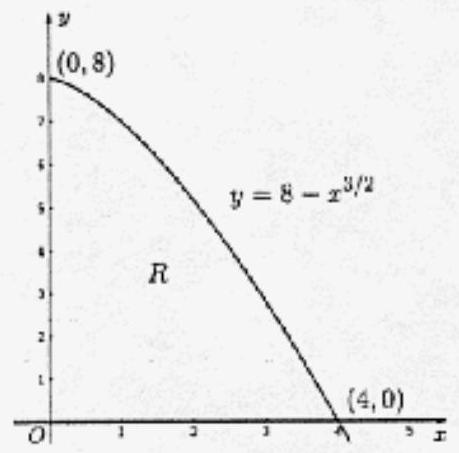
\includegraphics[width=0.6\linewidth]{figures/sg-bc-1998_fig1.jpg}
\[\begin{aligned}
A & =\int_{0}^{4}\left(8-x^{3 / 2}\right) d x \\
& =8 x-\left.\frac{2}{5} x^{5 / 2}\right|_{0} ^{4}=32-\frac{64}{5}=\frac{96}{5}=19.2
\end{aligned}\]
\begin{parts}
\part $\quad V=\pi \int_{0}^{4}\left(8-x^{3 / 2}\right)^{2} d x$

\[=\frac{576 \pi}{5}=115.2 \pi \approx 361.911\]
\part $\pi \int_{0}^{k}\left(8-x^{3 / 2}\right)^{2} d x=\frac{115.2 \pi}{2}$

\[\begin{aligned}
& {\left[\pi \int_{0}^{k}\left(8-x^{3 / 2}\right)^{2} d x=\pi \int_{k}^{4}\left(8-x^{3 / 2}\right)^{2} d x\right]} \\
& \int_{0}^{k}\left(8-x^{3 / 2}\right)^{2} d x=57.6 \\
& \int_{0}^{k}\left(64-16 x^{3 / 2}+x^{3}\right) d x=57.6 \\
& 64 k-\frac{32}{5} k^{5 / 2}+\frac{k^{4}}{4}=57.6 \\
& k \approx 0.995 \text { or } 0.994
\end{aligned}\]
\end{parts}
\par\medskip
\textbf{Rubric:}\par
\begin{parts}
\part $3\left\{\begin{aligned}
2: & \text { integral } \\
1: & \text { integrand } \\
1: & \text { limits } \\
1: & \text { answer }
\end{aligned}\right.$
\part $3\left\{\begin{aligned}
\text { 2: integral } & \\
& 1: \text { integrand } \\
& 1: \text { limits and constant } \\
1: & \text { answer }
\end{aligned}\right.$
\part $3\left\{\begin{array}{l}
1: \text { integral with } k \text { in limits } \\
1: \text { equates volumes } \\
1: \text { answer }
\end{array}\right.$
\part Note: 0/1 for answer in each part if no setup points earned
\end{parts}
\end{solution}

\question
% Q2 | 1998 Calculus BC | Part A | Calculator Active
Let $f$ be the function given by $f(x)=2 x e^{2 x}$.\\
\begin{parts}
\part Find $\lim _{x \rightarrow-\infty} f(x)$ and $\lim _{x \rightarrow \infty} f(x)$.
\part Find the absolute minimum value of $f$. Justify that your answer is an absolute minimum.
\part What is the range of $f$ ?
\part Consider the family of functions defined by $y=b x e^{b x}$, where $b$ is a nonzero constant. Show that the absolute minimum value of $b x e^{b x}$ is the same for all nonzero values of $b$.
\end{parts}
\begin{solution}
\begin{parts}
\part $\lim _{x \rightarrow-\infty} 2 x e^{2 z}=0$\\
$\lim _{x \rightarrow \infty} 2 x e^{2 x}=\infty$ or DNE
\part $f^{\prime}(x)=2 e^{2 x}+2 x \cdot 2 \cdot e^{2 x}=2 e^{2 x}(1+2 x)=0$ if $x=-1 / 2$\\
$f(-1 / 2)=-1 / e$ or -0.368 or -0.367\\
$-1 / e$ is an absolute minimum value because:\\
(i) $f^{\prime}(x)<0$ for all $x<-1 / 2$ and $f^{\prime}(x)>0$ for all $x>-1 / 2$\\
-or-\\
(ii) $f^{\prime}(x)-\frac{+}{-1 / 2}$\\
and $x=-1 / 2$ is the only critical number
\part Range of $f=[-1 / e, \infty)$\\
or $[-0.367, \infty)$\\
or $[-0.368, \infty)$
\part $y^{\prime}=b e^{b x}+b^{2} x e^{b z}=b e^{b x}(1+b x)=0$\\
if $x=-1 / b$\\
At $x=-1 / b, y=-1 / e$\\
$y$ has an absolute minimum value of $-1 / e$ for all nonzero $b$
\end{parts}
\par\medskip
\textbf{Rubric:}\par
\begin{parts}
\part $2\left\{\begin{array}{l}1: 0 \text { as } x \rightarrow-\infty \\ 1: \infty \text { or DNE as } x \rightarrow \infty\end{array}\right.$
\part $3\left\{\begin{array}{l}1: \text { solves } f^{\prime}(x)=0 \\ 1: \text { evaluates } f \text { at student's critical point } \\ 0 / 1 \text { if not local minimum from } \\ \text { student's derivative } \\ 1: \text { justifies absolute minimum value } \\ 0 / 1 \text { for a local argument } \\ 0 / 1 \text { without explicit symbolic } \\ \text { derivative }\end{array}\right.$
\part Note: $0 / 3$ if no absolute minimum based on student's derivative
\part 1: answer
\part Note: must include the left-hand endpoint; exclude the right-hand "endpoint"
\part $3\left\{\begin{array}{l}1: \text { sets } y^{\prime}=b e^{b z}(1+b x)=0 \\ 1: \text { solves student's } y^{\prime}=0 \\ 1: \text { evaluates } y \text { at a critical number } \\ \text { and gets a value independent of } b\end{array}\right.$
\part Note: 0/3 if only considering specific values of $b$
\end{parts}
\end{solution}

\question
% Q3 | 1998 Calculus BC | Part A | Calculator Active
Let $f$ be a function that has derivatives of all orders for all real numbers. Assume $f(0)=5$, $f^{\prime}(0)=-3, f^{\prime \prime}(0)=1$, and $f^{\prime \prime \prime}(0)=4$.\\
\begin{parts}
\part Write the third-degree Taylor polynomial for $f$ about $x=0$ and use it to approximate $f(0.2)$.
\part Write the fourth-degree Taylor polynomial for $g$, where $g(x)=f\left(x^{2}\right)$, about $x=0$.
\part Write the third-degree Taylor polynomial for $h$, where $h(x)=\int_{0}^{x} f(t) d t$, about $x=0$.
\part Let $h$ be defined as in part (c). Given that $f(1)=3$, either find the exact value of $h(1)$ or explain why it cannot be determined.
\end{parts}
\begin{solution}
\begin{parts}
\part $\quad P_{3}(f)(x)=5-3 x+\frac{1}{2} x^{2}+\frac{2}{3} x^{3}$

\begin{align*}f(0.2) \approx & P_{3}(f)(0.2)= \\
& 5-3(0.2)+\frac{0.04}{2}+\frac{2(0.008)}{3}= \\
& 4.425\end{align*}
\part $\quad P_{4}(g)(x)=P_{2}(f)\left(x^{2}\right)=5-3 x^{2}+\frac{1}{2} x^{4}$
\part $P_{3}(h)(x)=\int_{0}^{x}\left(5-3 t+\frac{1}{2} t^{2}\right) d t$

\[\begin{aligned}
& =\left[5 t-\frac{3}{2} t^{2}+\frac{1}{6} t^{3}\right]_{0}^{x} \\
& =5 x-\frac{3}{2} x^{2}+\frac{1}{6} x^{3}
\end{aligned}\]
\part $\quad h(1)=\int_{0}^{1} f(t) d t$\\
cannot be determined because $f(t)$ is known only for $t=0$ and $t=1$
\end{parts}
\par\medskip
\textbf{Rubric:}\par
\begin{parts}
\part $3\left\{\begin{aligned}
2: & 5-3 x+\frac{1}{2} x^{2}+\frac{2}{3} x^{3} \\
& <-1>\text { each incorrect term, } \\
& \text { extra term, or }+\cdots \\
1: & \text { approximates } f(0.2)
\end{aligned}\right.$
\part 2: $P_{2}(f)\left(x^{2}\right)$
\part $2\left\{\begin{array}{l}1: P_{3}(h)(x)=\int_{0}^{x} P_{2}(f)(t) d t \\ 1: \text { answer } \\ 0 / 1 \text { if any incorrect or extra terms }\end{array}\right.$
\part $2\left\{\begin{array}{l}1: h(1) \text { cannot be determined } \\ 1: \text { reason }\end{array}\right.$
\end{parts}
\end{solution}

\question
% Q4 | 1998 Calculus BC | Part B | Calculator Prohibited
Consider the differential equation given by $\frac{d y}{d x}=\frac{x y}{2}$.\\
\begin{parts}
\part On the axes provided below, sketch a slope field for the given differential equation at the nine points indicated.\\
\begin{center}
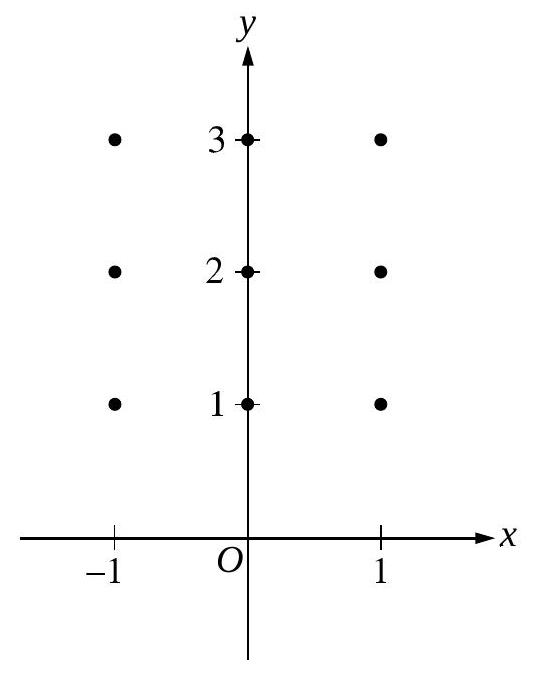
\includegraphics[width=0.6\linewidth]{figures/bc-1998_fig1.jpg}
\end{center}
\part Let $y=f(x)$ be the particular solution to the given differential equation with the initial condition $f(0)=3$. Use Euler's method starting at $x=0$, with a step size of 0.1 , to approximate $f(0.2)$. Show the work that leads to your answer.
\part Find the particular solution $y=f(x)$ to the given differential equation with the initial condition $f(0)=3$. Use your solution to find $f(0.2)$.
\end{parts}
\begin{solution}
(a)\\
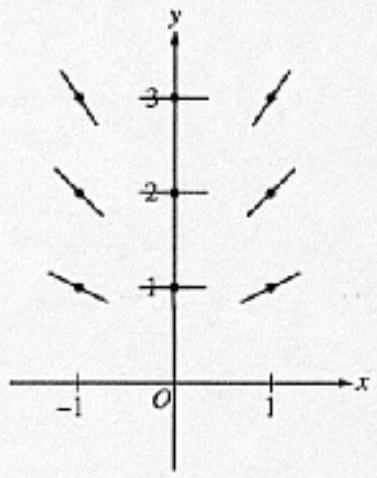
\includegraphics[width=0.6\linewidth]{figures/sg-bc-1998_fig2.jpg}\\
\begin{parts}
\part $f(0.1) \approx f(0)+f^{\prime}(0)(0.1)$

\begin{align*}& =3+\frac{1}{2}(0)(3)(0.1)=3 \\
f(0.2) & \approx f(0.1)+f^{\prime}(0.1)(0.1) \\
& =3+\frac{1}{2}(0.1)(3)(0.1) \\
& =3+\frac{.03}{2}=3.015\end{align*}
\part $\frac{d y}{d x}=\frac{x y}{2}$\\
$\int \frac{d y}{y}=\int \frac{x}{2} d x$\\
$\ln |y|=\frac{1}{4} x^{2}+C_{1}$\\
$y=C e^{x^{2} / 4}$\\
$3=C e^{0} \Longrightarrow C=3$\\
$y=3 e^{x^{2} / 4}$\\
$f(0.2)=3 e^{.04 / 4}=3 e^{.01}=3.030$
\end{parts}
\par\medskip
\textbf{Rubric:}\par
\begin{parts}
\part 1: line segments at nine points with negative - zero - positive slope left to right and increasing steepness bottom to top at $x=1$ and $x=-1$
\part $2\left\{\begin{array}{l}1: \text { Euler's Method equations } \\ \text { or equivalent table }\end{array}\right\} \begin{aligned} & 1: \text { answer } \\ & \text { (not eligible without first point) }\end{aligned}$
\part $6\left\{\begin{array}{l}\text { 1: separates variables } \\ \text { 1: antiderivative of } d y \text { term } \\ \text { 1: antiderivative of } d x \text { term } \\ \text { 1: solves for } y \\ \text { 1: solves for constant of integration } \\ \text { 1: evaluates } f(0.2)\end{array}\right.$
\part Note: $\max 4 / 6$ [1-1-1-0-0-1] if no constant of integration
\end{parts}
\end{solution}

\question
% Q5 | 1998 Calculus BC | Part B | Calculator Prohibited
The temperature outside a house during a 24 -hour period is given by
\[F(t)=80-10 \cos \left(\frac{\pi t}{12}\right), 0 \leq t \leq 24,\]

where $F(t)$ is measured in degrees Fahrenheit and $t$ is measured in hours.\\
\begin{parts}
\part Sketch the graph of $F$ on the grid below.\\
\begin{center}
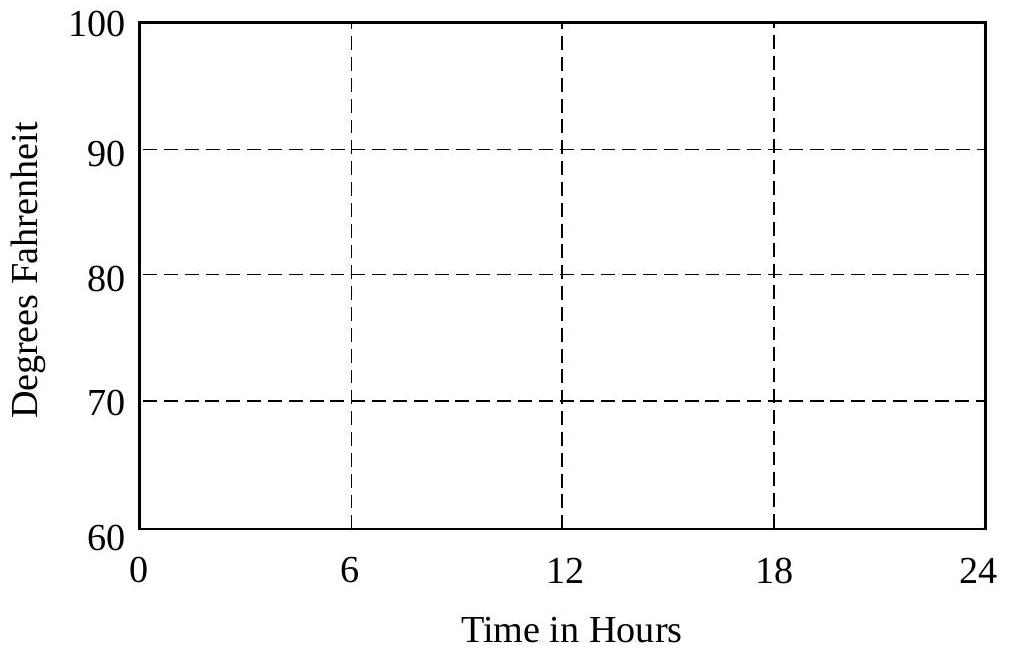
\includegraphics[width=0.6\linewidth]{figures/bc-1998_fig2.jpg}
\end{center}
\part Find the average temperature, to the nearest degree Fahrenheit, between $t=6$ and $t=14$.
\part An air conditioner cooled the house whenever the outside temperature was at or above 78 degrees Fahrenheit. For what values of $t$ was the air conditioner cooling the house?
\part The cost of cooling the house accumulates at the rate of $\$ 0.05$ per hour for each degree the outside temperature exceeds 78 degrees Fahrenheit. What was the total cost, to the nearest cent, to cool the house for this 24 -hour period?
\end{parts}
\begin{solution}
(a)\\
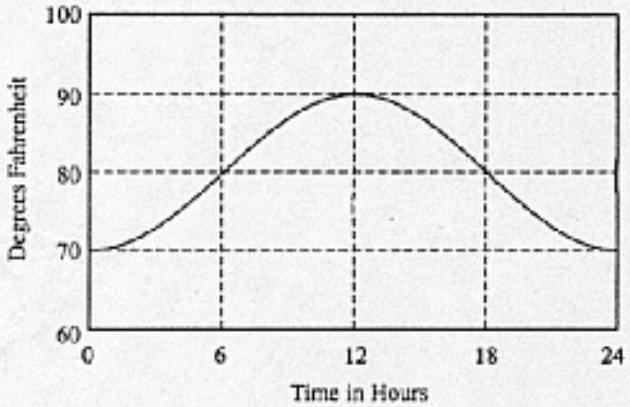
\includegraphics[width=0.6\linewidth]{figures/sg-bc-1998_fig3.jpg}\\
\begin{parts}
\part Avg. $=\frac{1}{14-6} \int_{6}^{14}\left[80-10 \cos \left(\frac{\pi t}{12}\right)\right] d t$

\begin{align*}& =\frac{1}{8}(697.2957795) \\
& =87.162 \text { or } 87.161 \\
& \approx 87^{\circ} \mathrm{F}\end{align*}
\part $\left[80-10 \cos \left(\frac{\pi t}{12}\right)\right]-78 \geq 0$\\
$2-10 \cos \left(\frac{\pi t}{12}\right) \geq 0$\\
$\left.\begin{array}{c}5.230 \\ \text { or } \\ 5.231\end{array}\right\} \leq t \leq\left\{\begin{array}{c}18.769 \\ \text { or } \\ 18.770\end{array}\right.$

\[18.770\]
\part $C=0.05 \int_{\substack{5.231 \\ \text { or } \\ 5.230}}^{18.769}\left(\left[80-10 \cos \left(\frac{\pi t}{12}\right)\right]-78\right) d t$

\[=0.05(101.92741)=5.096 \approx \$ 5.10\]
\end{parts}
\par\medskip
\textbf{Rubric:}\par
\begin{parts}
\part 1: bell-shaped graph
\part $3\left\{\begin{array}{l}
\text { 2: integral } \\
\text { 1: limits and } 1 /(14-6) \\
\text { 1: integrand } \\
\text { 1: answer } \\
0 / 1 \text { if integral not of the form } \\
\frac{1}{b-a} \int_{a}^{b} F(t) d t
\end{array}\right.$
\part $2\left\{\begin{array}{l}1: \text { inequality or equation } \\ 1: \text { solutions with interval }\end{array}\right.$
\part $3\left\{\begin{array}{l}\text { 2: integral } \\ \text { 1: limits and } 0.05 \\ \text { 1: integrand } \\ \text { 1: answer } \\ 0 / 1 \text { if integral not of the form } \\ k \int_{a}^{b}(F(t)-78) d t\end{array}\right.$
\end{parts}
\end{solution}

\question
% Q6 | 1998 Calculus BC | Part B | Calculator Prohibited
A particle moves along the curve defined by the equation $y=x^{3}-3 x$. The $x$-coordinate of the particle, $x(t)$, satisfies the equation $\frac{d x}{d t}=\frac{1}{\sqrt{2 t+1}}$, for $t \geq 0$ with initial condition $x(0)=-4$.\\
\begin{parts}
\part Find $x(t)$ in terms of $t$.
\part Find $\frac{d y}{d t}$ in terms of $t$.
\part Find the location and speed of the particle at time $t=4$.
\end{parts}
\begin{solution}
\begin{parts}
\part $\quad x(t)=\int \frac{1}{\sqrt{2 t+1}} d t$
\begin{align*}& x(t)=\sqrt{2 t+1}+C \\
& x(0)=-4=1+C \Rightarrow C=-5 \\
& x(t)=\sqrt{2 t+1}-5\end{align*}

\[3\left\{\begin{array}{l}
1: x(t)=\int \frac{d t}{\sqrt{2 t+1}} \\
1: x(t)=\sqrt{2 t+1}+C \\
1: \text { evaluates } C
\end{array}\right.\]

2: answer

\[<-1>\text { each error }\]

Note: failure to express $\frac{d y}{d t}$ solely in terms of $t$ is a single error

\[4\left\{\begin{array}{l}
1: \text { position } \\
1: \text { evaluates } \frac{d x}{d t} \text { and } \frac{d y}{d t} \text { at } t=4 \\
1: \text { uses speed formula } \\
1: \text { answer }
\end{array}\right.\]
\part $y=x^{3}-3 x$

\[\begin{aligned}
\frac{d y}{d t} & =3 x^{2} \frac{d x}{d t}-3 \frac{d x}{d t} \\
& =\left(3 x^{2}-3\right) \frac{d x}{d t} \\
& =\left[3(\sqrt{2 t+1}-5)^{2}-3\right]\left[\frac{1}{\sqrt{2 t+1}}\right]
\end{aligned}\]
\part $x(4)=\sqrt{9}-5=-2$

\[y(4)=(-2)^{3}-3(-2)=-2\]

Location at $t=4$ is $(-2,-2)$

\[\begin{aligned}
& \left.\frac{d x}{d t}\right|_{t=4}=\frac{1}{3} \\
& \left.\frac{d y}{d t}\right|_{t=4}=\frac{3(3-5)^{2}-3}{3}=3 \\
& \text { Speed }=\sqrt{\left(\frac{1}{3}\right)^{2}+3^{2}}=\sqrt{\frac{82}{9}}=3.018
\end{aligned}\]
\end{parts}
\end{solution}

\end{questions}

\section*{1999 AP Calculus BC}

\begin{questions}

\question
% Q1 | 1999 Calculus BC | Part A | Calculator Active
A particle moves in the $x y$-plane so that its position at any time $t, 0 \leq t \leq \pi$, is given by $x(t)=\frac{t^{2}}{2}-\ln (1+t)$ and $y(t)=3 \sin t$.\\
\begin{parts}
\part Sketch the path of the particle in the $x y$-plane below. Indicate the direction of motion along the path.\\
\begin{center}
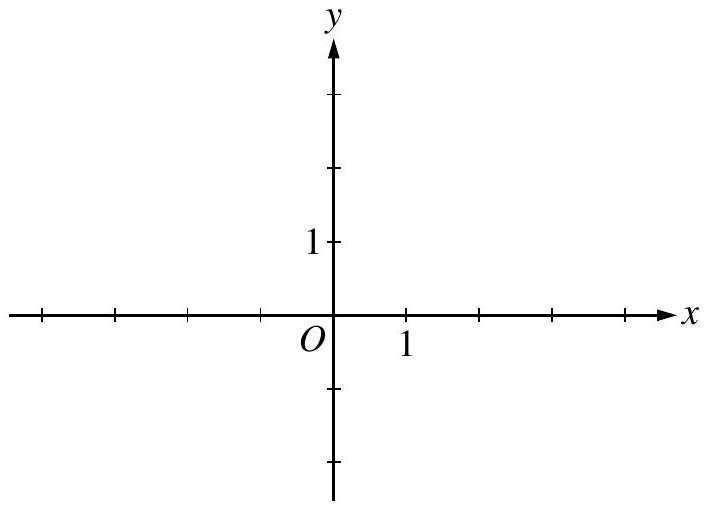
\includegraphics[width=0.6\linewidth]{figures/bc-1999_fig1.jpg}
\end{center}
\part At what time $t, 0 \leq t \leq \pi$, does $x(t)$ attain its minimum value? What is the position $(x(t), y(t))$ of the particle at this time?
\part At what time $t, 0<t<\pi$, is the particle on the $y$-axis? Find the speed and the acceleration vector of the particle at this time.
\end{parts}
\begin{solution}
(a)\\
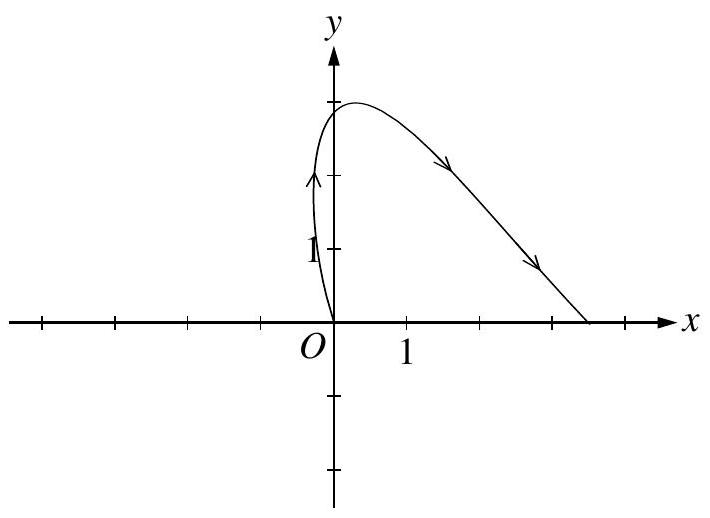
\includegraphics[width=0.6\linewidth]{figures/sg-bc-1999_fig1.jpg}\\
\begin{parts}
\part $x^{\prime}(t)=t-\frac{1}{1+t}=0$
\end{parts}
\end{solution}

\question
% Q2 | 1999 Calculus BC | Part A | Calculator Active
\begin{center}
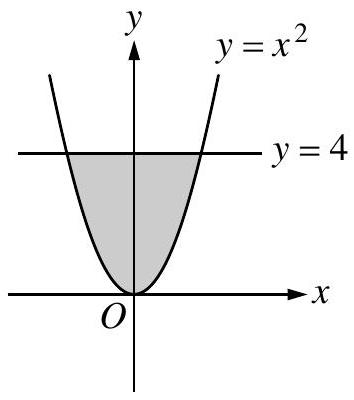
\includegraphics[width=0.6\linewidth]{figures/bc-1999_fig2.jpg}
\end{center}
The shaded region, $R$, is bounded by the graph of $y=x^{2}$ and the line $y=4$, as shown in the figure above.\\
\begin{parts}
\part Find the area of $R$.
\part Find the volume of the solid generated by revolving $R$ about the $x$-axis.
\part There exists a number $k, k>4$, such that when $R$ is revolved about the line $y=k$, the resulting solid has the same volume as the solid in part (b). Write, but do not solve, an equation involving an integral expression that can be used to find the value of $k$.
\end{parts}

\question
% Q3 | 1999 Calculus BC | Part A | Calculator Active
\begin{center}
\begin{tabular}{c|c}
\begin{tabular}{c}
$t$ \\
(hours) \\
\end{tabular} & \begin{tabular}{c}
$R(t)$ \\
(gallons per hour) \\
\end{tabular} \\
\hline
0 & 9.6 \\
3 & 10.4 \\
6 & 10.8 \\
9 & 11.2 \\
12 & 11.4 \\
15 & 11.3 \\
18 & 10.7 \\
21 & 10.2 \\
24 & 9.6 \\
\end{tabular}
\end{center}
The rate at which water flows out of a pipe, in gallons per hour, is given by a differentiable function $R$ of time $t$. The table above shows the rate as measured every 3 hours for a 24 -hour period.\\
\begin{parts}
\part Use a midpoint Riemann sum with 4 subdivisions of equal length to approximate $\int_{0}^{24} R(t) d t$. Using correct units, explain the meaning of your answer in terms of water flow.
\part Is there some time $t, 0<t<24$, such that $R^{\prime}(t)=0$ ? Justify your answer.
\part The rate of water flow $R(t)$ can be approximated by $Q(t)=\frac{1}{79}\left(768+23 t-t^{2}\right)$. Use $Q(t)$ to approximate the average rate of water flow during the 24 -hour time period. Indicate units of measure.
\end{parts}
\begin{solution}
\begin{parts}
\part Area $=\int_{-2}^{2}\left(4-x^{2}\right) d x$
\[\begin{aligned}
& =2 \int_{0}^{2}\left(4-x^{2}\right) d x \\
& =2\left[4 x-\frac{x^{3}}{3}\right]_{0}^{2} \\
& =\frac{32}{3}=10.666 \text { or } 10.667
\end{aligned}\]
\part Volume $=\pi \int_{-2}^{2}\left(4^{2}-\left(x^{2}\right)^{2}\right) d x$

\[\begin{aligned}
& =2 \pi \int_{0}^{2}\left(16-x^{4}\right) d x \\
& =2 \pi\left[16 x-\frac{x^{5}}{5}\right]_{0}^{2} \\
& =\frac{256 \pi}{5}=160.849 \text { or } 160.850
\end{aligned}\]
\part $\pi \int_{-2}^{2}\left[\left(k-x^{2}\right)^{2}-(k-4)^{2}\right] d x=\frac{256 \pi}{5}$

\[2\left\{\begin{array}{l}
1 \text { : integral } \\
1 \text { : answer }
\end{array}\right.\]

$3\left\{\begin{array}{l}1 \text { : limits and constant } \\ 1 \text { : integrand } \\ 1 \text { : answer }\end{array}\right.$

\[4\left\{\begin{aligned}
1: & \text { limits and constant } \\
2: & \text { integrand } \\
& <-1>\text { each error } \\
1: & \text { equation }
\end{aligned}\right.\]
The rate at which water flows out of a pipe, in gallons per hour, is given by a differentiable function $R$ of time $t$. The table above shows the rate as measured every 3 hours for a 24 -hour period.
\part Use a midpoint Riemann sum with 4 subdivisions of equal length to approximate $\int_{0}^{24} R(t) d t$. Using correct units, explain the meaning of your answer in terms of water flow.
\part Is there some time $t, 0<t<24$, such that $R^{\prime}(t)=0$ ? Justify your answer.
\part The rate of water flow $R(t)$ can be approximated by $Q(t)=\frac{1}{79}\left(768+23 t-t^{2}\right)$. Use $Q(t)$ to approximate the
\begin{center}
\begin{tabular}{c|c}
\begin{tabular}{c}
$t$ \\
(hours) \\
\end{tabular} & \begin{tabular}{c}
$R(t)$ \\
(gallons per hour) \\
\end{tabular} \\
\hline
0 & 9.6 \\
3 & 10.4 \\
6 & 10.8 \\
9 & 11.2 \\
12 & 11.4 \\
15 & 11.3 \\
18 & 10.7 \\
21 & 10.2 \\
24 & 9.6 \\
\end{tabular}
\end{center}

average rate of water flow during the 24 -hour time period. Indicate units of measure.
\part $\int_{0}^{24} R(t) d t \approx 6[R(3)+R(9)+R(15)+R(21)]$

\begin{align*}& =6[10.4+11.2+11.3+10.2] \\
& =258.6 \text { gallons }\end{align*}

This is an approximation to the total flow in gallons of water from the pipe in the 24 -hour period.
\part Yes;

Since $R(0)=R(24)=9.6$, the Mean Value Theorem guarantees that there is a $t, 0<t<24$, such that $R^{\prime}(t)=0$.
\part Average rate of flow\\
$\approx$ average value of $Q(t)$

\[\begin{aligned}
& =\frac{1}{24} \int_{0}^{24} \frac{1}{79}\left(768+23 t-t^{2}\right) d t \\
& =10.785 \mathrm{gal} / \mathrm{hr} \text { or } 10.784 \mathrm{gal} / \mathrm{hr}
\end{aligned}\]

(units) Gallons in part (a) and gallons/hr in part (c), or equivalent.
\end{parts}
\par\medskip
\textbf{Rubric:}\par
\begin{parts}
\part $3\left\{\begin{array}{l}1: R(3)+R(9)+R(15)+R(21) \\ 1: \text { answer } \\ 1: \text { explanation }\end{array}\right.$
\part $2\left\{\begin{array}{l}1: \text { answer } \\ 1: \text { MVT or equivalent }\end{array}\right.$
\part $3\left\{\begin{array}{l}1: \text { limits and average value constant } \\ 1: Q(t) \text { as integrand } \\ 1: \text { answer }\end{array}\right.$
\part 1: units
\end{parts}
\end{solution}

\question
% Q4 | 1999 Calculus BC | Part B | Calculator Prohibited
The function $f$ has derivatives of all orders for all real numbers $x$. Assume $f(2)=-3, f^{\prime}(2)=5, f^{\prime \prime}(2)=3$, and $f^{\prime \prime \prime}(2)=-8$.\\
\begin{parts}
\part Write the third-degree Taylor polynomial for $f$ about $x=2$ and use it to approximate $f(1.5)$.
\part The fourth derivative of $f$ satisfies the inequality $\left|f^{(4)}(x)\right| \leq 3$ for all $x$ in the closed interval [1.5,2]. Use the Lagrange error bound on the approximation to $f(1.5)$ found in part (a) to explain why $f(1.5) \neq-5$.
\part Write the fourth-degree Taylor polynomial, $P(x)$, for $g(x)=f\left(x^{2}+2\right)$ about $x=0$. Use $P$ to explain why $g$ must have a relative minimum at $x=0$.
\end{parts}
\begin{solution}
\begin{parts}
\part $\quad T_{3}(f, 2)(x)=-3+5(x-2)+\frac{3}{2}(x-2)^{2}-\frac{8}{6}(x-2)^{3}$

\begin{align*}f(1.5) \approx & T_{3}(f, 2)(1.5) \\
& =-3+5(-0.5)+\frac{3}{2}(-0.5)^{2}-\frac{4}{3}(-0.5)^{3} \\
& =-4.958 \overline{3}=-4.958\end{align*}
\part Lagrange Error Bound $=\frac{3}{4!}|1.5-2|^{4}=0.0078125$\\
$f(1.5)>-4.958 \overline{3}-0.0078125=-4.966>-5$\\
Therefore, $f(1.5) \neq-5$.
\part $P(x)=T_{4}(g, 0)(x)$

\[=T_{2}(f, 2)\left(x^{2}+2\right)=-3+5 x^{2}+\frac{3}{2} x^{4}\]

The coefficient of $x$ in $P(x)$ is $g^{\prime}(0)$. This coefficient is 0 , so $g^{\prime}(0)=0$.

The coefficient of $x^{2}$ in $P(x)$ is $\frac{g^{\prime \prime}(0)}{2!}$. This coefficient is 5 , so $g^{\prime \prime}(0)=10$ which is greater than 0 .

Therefore, $g$ has a relative minimum at $x=0$.
\end{parts}
\par\medskip
\textbf{Rubric:}\par
\begin{parts}
\part $4\left\{\begin{aligned} 3: & T_{3}(f, 2)(x) \\ & <-1>\text { each error } \\ 1: & \text { approximation of } f(1.5)\end{aligned}\right.$
\part $2\left\{\begin{array}{l}\text { 1: value of Lagrange Error Bound } \\ \text { 1: explanation }\end{array}\right.$
\part $3\left\{\begin{aligned} 2: & T_{4}(g, 0)(x) \\ & <-1>\text { each incorrect, missing, } \\ & \text { or extra term } \\ 1: & \text { explanation }\end{aligned}\right.$
\part Note:
\end{parts}
\end{solution}

\question
% Q5 | 1999 Calculus BC | Part B | Calculator Prohibited
\begin{center}
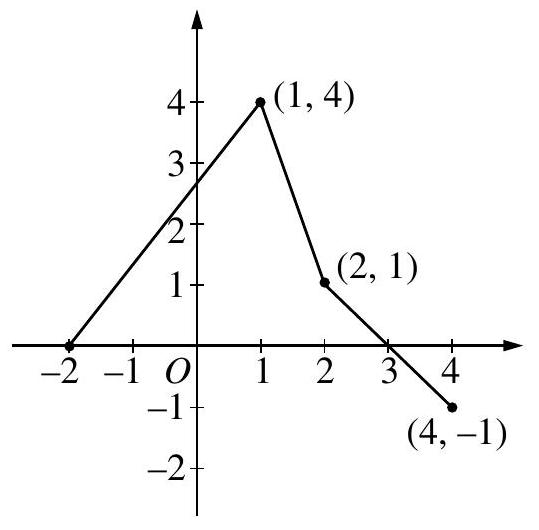
\includegraphics[width=0.6\linewidth]{figures/bc-1999_fig3.jpg}
\end{center}
The graph of the function $f$, consisting of three line segments, is given above. Let $g(x)=\int_{1}^{x} f(t) d t$.\\
\begin{parts}
\part Compute $g(4)$ and $g(-2)$.
\part Find the instantaneous rate of change of $g$, with respect to $x$, at $x=1$.
\part Find the absolute minimum value of $g$ on the closed interval $[-2,4]$. Justify your answer.
\part The second derivative of $g$ is not defined at $x=1$ and $x=2$. How many of these values are $x$-coordinates of points of inflection of the graph of $g$ ? Justify your answer.
\end{parts}
\begin{solution}
\begin{parts}
\part $g(4)=\int_{1}^{4} f(t) d t=\frac{3}{2}+1+\frac{1}{2}-\frac{1}{2}=\frac{5}{2}$\\
$g(-2)=\int_{1}^{-2} f(t) d t=-\frac{1}{2}(12)=-6$
\part $g^{\prime}(1)=f(1)=4$
\part $g$ is increasing on $[-2,3]$ and decreasing on $[3,4]$.

Therefore, $g$ has absolute minimum at an endpoint of $[-2,4]$.\\
Since $g(-2)=-6$ and $g(4)=\frac{5}{2}$,\\
the absolute minimum value is -6 .
\part One; $x=1$

On $(-2,1), g^{\prime \prime}(x)=f^{\prime}(x)>0$\\
On $(1,2), g^{\prime \prime}(x)=f^{\prime}(x)<0$\\
On $(2,4), g^{\prime \prime}(x)=f^{\prime}(x)<0$\\
Therefore ( $1, g(1)$ ) is a point of inflection and ( $2, g(2)$ ) is not.
\end{parts}
\par\medskip
\textbf{Rubric:}\par
\begin{parts}
\part $2\left\{\begin{array}{l}1: g(4) \\ 1: g(-2)\end{array}\right.$
\part 1: answer
\part $3\left\{\begin{array}{l}1 \text { : interior analysis } \\ 1 \text { : endpoint analysis } \\ 1 \text { : answer }\end{array}\right.$
\part 3 $\left\{\begin{array}{l}1 \text { : choice of } x=1 \text { only } \\ 1 \text { : show }(1, g(1)) \text { is a point of inflection } \\ 1 \text { : show }(2, g(2)) \text { is not a point of inflection }\end{array}\right.$
\end{parts}
\end{solution}

\question
% Q6 | 1999 Calculus BC | Part B | Calculator Prohibited
Let $f$ be the function whose graph goes through the point $(3,6)$ and whose derivative is given by $f^{\prime}(x)=\frac{1+e^{x}}{x^{2}}$.\\
\begin{parts}
\part Write an equation of the line tangent to the graph of $f$ at $x=3$ and use it to approximate $f$ (3.1).
\part Use Euler's method, starting at $x=3$ with a step size of 0.05 , to approximate $f(3.1)$. Use $f^{\prime \prime}$ to explain why this approximation is less than $f(3.1)$.
\part Use $\int_{3}^{3.1} f^{\prime}(x) d x$ to evaluate $f(3.1)$.
\end{parts}
\begin{solution}
\begin{parts}
\part $f^{\prime}(3)=\frac{1+e^{3}}{9}=2.342$ or 2.343

\begin{align*}& y-6=\frac{1+e^{3}}{9}(x-3) \\
& y=6+\frac{1+e^{3}}{9}(x-3) \\
& f(3.1) \approx 6+\frac{1+e^{3}}{9}(0.1)=6.234\end{align*}
\part $f(3.05) \approx f(3)+f^{\prime}(3)(0.05)$

\[=6+0.11714=6.11714\]

\begin{align*}f(3.1) & \approx 6.11714+f^{\prime}(3.05)(0.05) \\
& =6.11714+(2.37735)(0.05)=6.236\end{align*}

$f^{\prime \prime}(x)=\frac{x^{2} e^{x}-2 x\left(1+e^{x}\right)}{x^{4}}=\frac{(x-2) e^{x}-2}{x^{3}}$\\
For $x \geq 3, f^{\prime \prime}(x)>\frac{e^{x}-2}{x^{3}}>0$ and the graph of $f$ is concave upward on ( $3,3.1$ ). Therefore, the Euler approximation lines at 3 and 3.05 lie below the graph.
\part $f(3.1)-f(3)=\int_{3}^{3.1} \frac{1+e^{x}}{x^{2}} d x$

\[f(3.1)=6+0.2378=6.237 \text { or } 6.238\]
\end{parts}
\par\medskip
\textbf{Rubric:}\par
\begin{parts}
\part $3\left\{\begin{array}{l}1: f^{\prime}(3) \\ 1: \text { equation } \\ 1: \text { approximation of } f(3.1)\end{array}\right.$
\part $4\left\{\begin{array}{l}1: \quad \text { Euler's method equations or } \\ \quad \text { equivalent table } \\ 1: \quad \text { Euler approximation to } f(3.1) \\ \quad(\text { not eligible without first point }) \\ 1: f^{\prime \prime}(x) \\ 1: \text { reason }\end{array}\right.$
\part $2\left\{\begin{array}{l}1: \int_{3}^{3.1} \frac{1+e^{x}}{x^{2}} d x=f(3.1)-f(3) \\ 1: \text { answer }\end{array}\right.$
\end{parts}
\end{solution}

\end{questions}

\section*{2000 AP Calculus BC}

\begin{questions}

\question
% Q1 | 2000 Calculus BC | Part A | Calculator Active
\begin{center}
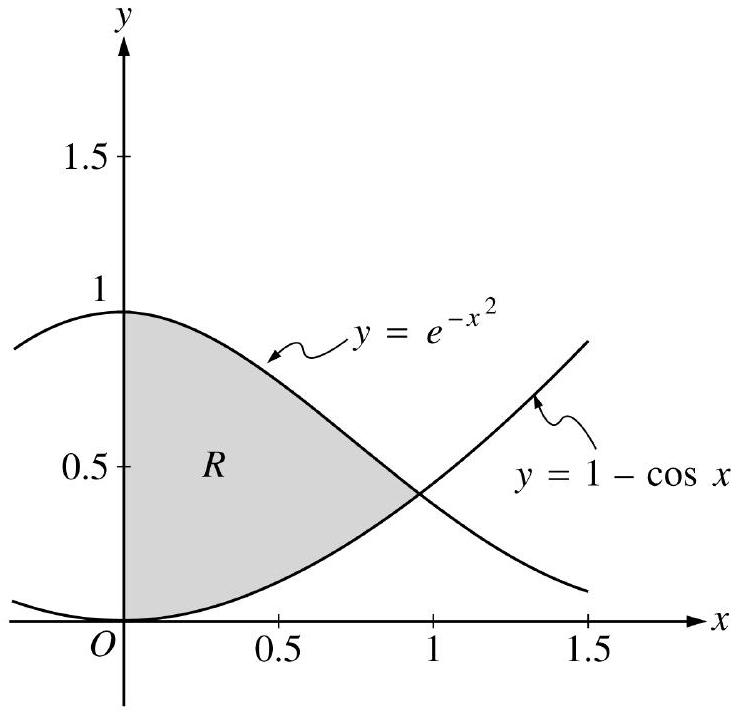
\includegraphics[width=0.6\linewidth]{figures/bc-2000_fig1.jpg}
\end{center}
Let $R$ be the shaded region in the first quadrant enclosed by the graphs of $y=e^{-x^{2}}, y=1-\cos x$, and the $y$-axis, as shown in the figure above.\\
\begin{parts}
\part Find the area of the region $R$.
\part Find the volume of the solid generated when the region $R$ is revolved about the $x$-axis.
\part The region $R$ is the base of a solid. For this solid, each cross section perpendicular to the $x$-axis is a square. Find the volume of this solid.
\end{parts}
\begin{solution}
\begin{parts}
\part $y^{2}+2 x y \frac{d y}{d x}-3 x^{2} y-x^{3} \frac{d y}{d x}=0$

\[\frac{d y}{d x}\left(2 x y-x^{3}\right)=3 x^{2} y-y^{2}\]

\[\frac{d y}{d x}=\frac{3 x^{2} y-y^{2}}{2 x y-x^{3}}\]
\part When $x=1, y^{2}-y=6$

\begin{align*}& y^{2}-y-6=0 \\
& (y-3)(y+2)=0 \\
& y=3, y=-2\end{align*}

At $(1,3), \frac{d y}{d x}=\frac{9-9}{6-1}=0$\\
Tangent line equation is $y=3$\\
At $(1,-2), \frac{d y}{d x}=\frac{-6-4}{-4-1}=\frac{-10}{-5}=2$\\
Tangent line equation is $y+2=2(x-1)$
\part Tangent line is vertical when $2 x y-x^{3}=0$

\[x\left(2 y-x^{2}\right)=0 \text { gives } x=0 \text { or } y=\frac{1}{2} x^{2}\]

There is no point on the curve with $x$-coordinate 0 .

When $y=\frac{1}{2} x^{2}, \frac{1}{4} x^{5}-\frac{1}{2} x^{5}=6$

\begin{align*}-\frac{1}{4} x^{5} & =6 \\
x & =\sqrt[5]{-24}\end{align*}

\[2\left\{\begin{array}{l}
1: \text { implicit differentiation } \\
1: \text { verifies expression for } \frac{d y}{d x}
\end{array}\right.\]

$4 \begin{cases}1: & y^{2}-y=6 \\ 1: & \text { solves for } y \\ 2: & \text { tangent lines }\end{cases}$\\
Note: $0 / 4$ if not solving an equation of the form $y^{2}-y=k$

\[3\left\{\begin{aligned}
1: & \text { sets denominator of } \frac{d y}{d x} \text { equal to } 0 \\
1: & \text { substitutes } y=\frac{1}{2} x^{2} \text { or } x= \pm \sqrt{2 y} \\
& \text { into the equation for the curve } \\
1: & \text { solves for } x \text {-coordinate }
\end{aligned}\right.\]

Consider the differential equation given by $\frac{d y}{d x}=x(y-1)^{2}$.
\part On the axes provided, sketch a slope field for the given differential equation at the eleven points indicated.
\part Use the slope field for the given differential equation to explain why a solution could not have the graph shown below.
\part Find the particular solution $y=f(x)$ to the given differential equation with the initial condition $f(0)=-1$.\\
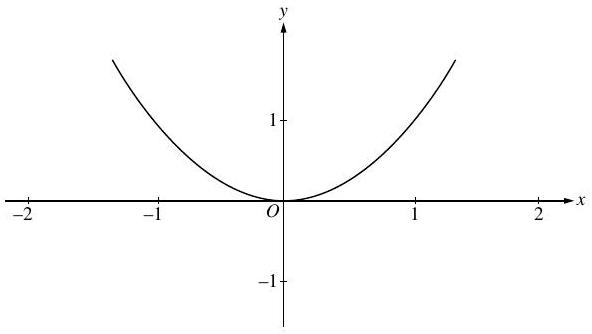
\includegraphics[width=0.6\linewidth]{figures/sg-bc-2000_fig3.jpg}
\part Find the range of the solution found in part (c).\\
(a)\\
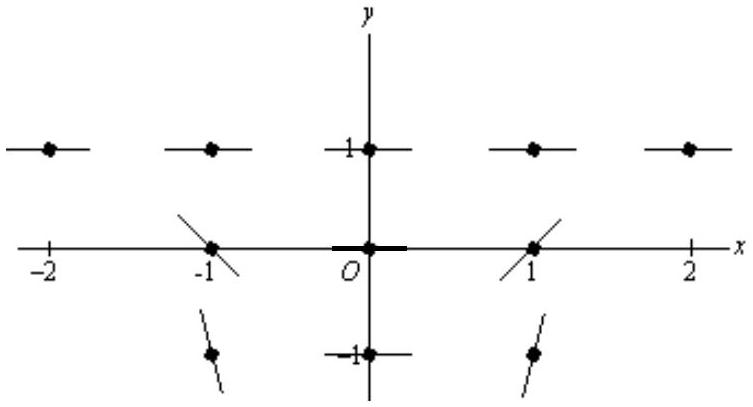
\includegraphics[width=0.6\linewidth]{figures/sg-bc-2000_fig4.jpg}
\part The graph does not have slope 0 where $y=1$. - or -

The slope field shown suggests that solutions are asymptotic to $y=1$ from below, but the graph does not exhibit this behavior.
\part $\frac{1}{(y-1)^{2}} d y=x d x$\\
$-\frac{1}{y-1}=\frac{1}{2} x^{2}+C$\\
$\frac{1}{2}=0+C ; \quad C=\frac{1}{2}$\\
$-\frac{1}{y-1}=\frac{1}{2}\left(x^{2}+1\right) ; \quad y=1-\frac{2}{x^{2}+1}$
\part range is $-1 \leq y<1$

\begin{verbatim}
    1 : zero slope at 7 points with
        $y=1$ and $x=0$
    1: negative slope at ( $-1,0$ ) and ( $-1,-1$ )
        positive slope at $(1,0)$ and $(1,-1)$
        steeper slope at $y=-1$ than $y=0$
    reason
\[5 \begin{cases}1: & \text { separates variables } \\ 1: & \text { antiderivatives } \\ 1: & \text { constant of integration } \\ 1: & \text { uses initial condition } f(0)=-1 \\ 1: & \text { solves for } y \\ & 0 / 1 \text { if } y \text { is linear }\end{cases}\]
    separates variables
    antiderivatives
    constant of integration
    uses initial condition $f(0)=-1$
    solves for $y$
    $0 / 1$ if $y$ is linear
\end{verbatim}
\end{parts}
\par\medskip
\textbf{Rubric:}\par
\begin{parts}
\part Note: $\max 2 / 5[1-1-0-0-0]$ if no constant of integration
\part Note: $0 / 5$ if no separation of variables
\end{parts}
\end{solution}

\question
% Q2 | 2000 Calculus BC | Part A | Calculator Active
\begin{center}
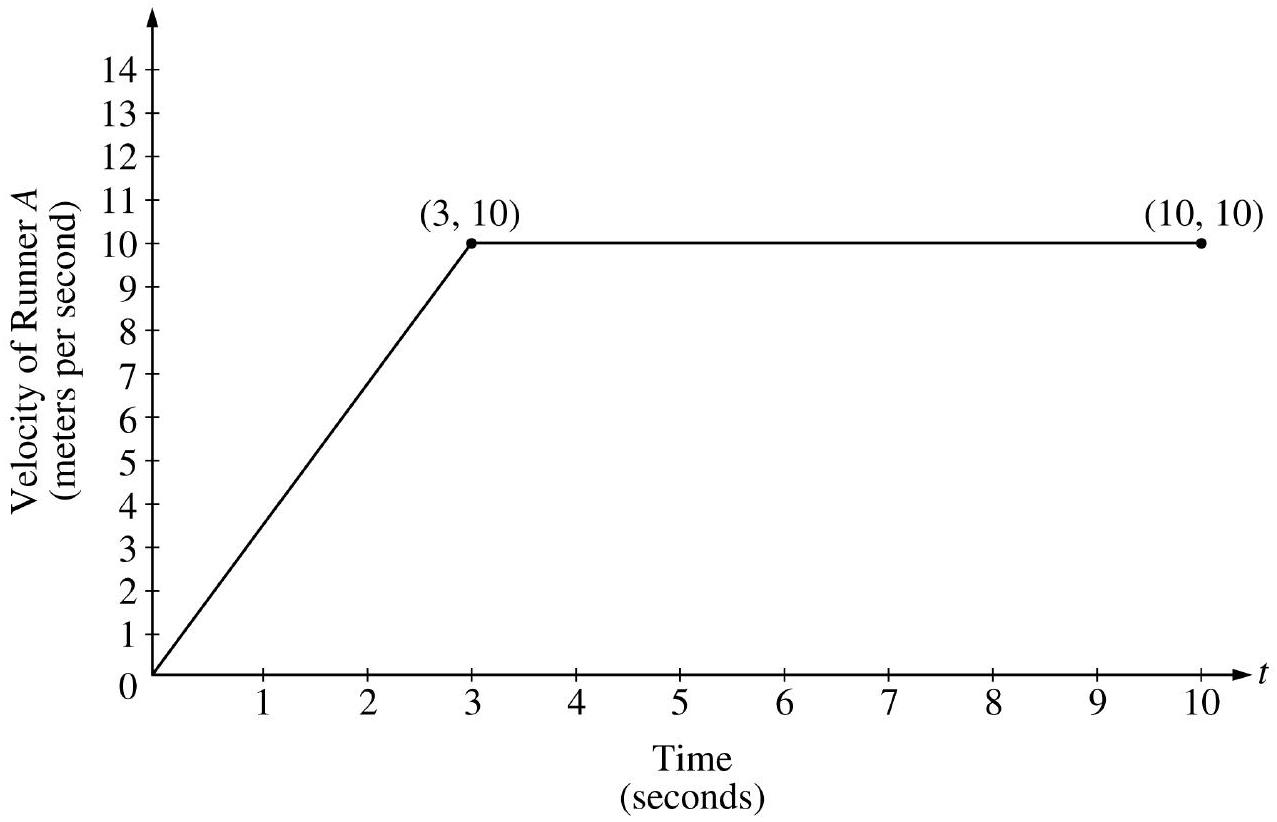
\includegraphics[width=0.6\linewidth]{figures/bc-2000_fig2.jpg}
\end{center}
Two runners, $A$ and $B$, run on a straight racetrack for $0 \leq t \leq 10$ seconds. The graph above, which consists of two line segments, shows the velocity, in meters per second, of Runner $A$. The velocity, in meters per second, of Runner $B$ is given by the function $v$ defined by $v(t)=\frac{24 t}{2 t+3}$.\\
\begin{parts}
\part Find the velocity of Runner $A$ and the velocity of Runner $B$ at time $t=2$ seconds. Indicate units of measure.
\part Find the acceleration of Runner $A$ and the acceleration of Runner $B$ at time $t=2$ seconds. Indicate units of measure.
\part Find the total distance run by Runner $A$ and the total distance run by Runner $B$ over the time interval $0 \leq t \leq 10$ seconds. Indicate units of measure.
\end{parts}

\question
% Q3 | 2000 Calculus BC | Part A | Calculator Active
The Taylor series about $x=5$ for a certain function $f$ converges to $f(x)$ for all $x$ in the interval of convergence. The $n$th derivative of $f$ at $x=5$ is given by $f^{(n)}(5)=\frac{(-1)^{n} n!}{2^{n}(n+2)}$, and $f(5)=\frac{1}{2}$.\\
\begin{parts}
\part Write the third-degree Taylor polynomial for $f$ about $x=5$.
\part Find the radius of convergence of the Taylor series for $f$ about $x=5$.
\part Show that the sixth-degree Taylor polynomial for $f$ about $x=5$ approximates $f(6)$ with error less than $\frac{1}{1000}$.
\end{parts}

\question
% Q4 | 2000 Calculus BC | Part B | Calculator Prohibited
A moving particle has position $(x(t), y(t))$ at time $t$. The position of the particle at time $t=1$ is $(2,6)$, and the velocity vector at any time $t>0$ is given by $\left(1-\frac{1}{t^{2}}, 2+\frac{1}{t^{2}}\right)$.\\
\begin{parts}
\part Find the acceleration vector at time $t=3$.
\part Find the position of the particle at time $t=3$.
\part For what time $t>0$ does the line tangent to the path of the particle at $(x(t), y(t))$ have a slope of 8 ?
\part The particle approaches a line as $t \rightarrow \infty$. Find the slope of this line. Show the work that leads to your conclusion.
\end{parts}

\question
% Q5 | 2000 Calculus BC | Part B | Calculator Prohibited
Consider the curve given by $x y^{2}-x^{3} y=6$.\\
\begin{parts}
\part Show that $\frac{d y}{d x}=\frac{3 x^{2} y-y^{2}}{2 x y-x^{3}}$.
\part Find all points on the curve whose $x$-coordinate is 1 , and write an equation for the tangent line at each of these points.
\part Find the $x$-coordinate of each point on the curve where the tangent line is vertical.
\end{parts}

\question
% Q6 | 2000 Calculus BC | Part B | Calculator Prohibited
Consider the differential equation given by $\frac{d y}{d x}=x(y-1)^{2}$.\\
\begin{parts}
\part On the axes provided, sketch a slope field for the given differential equation at the eleven points indicated.\\
\begin{center}
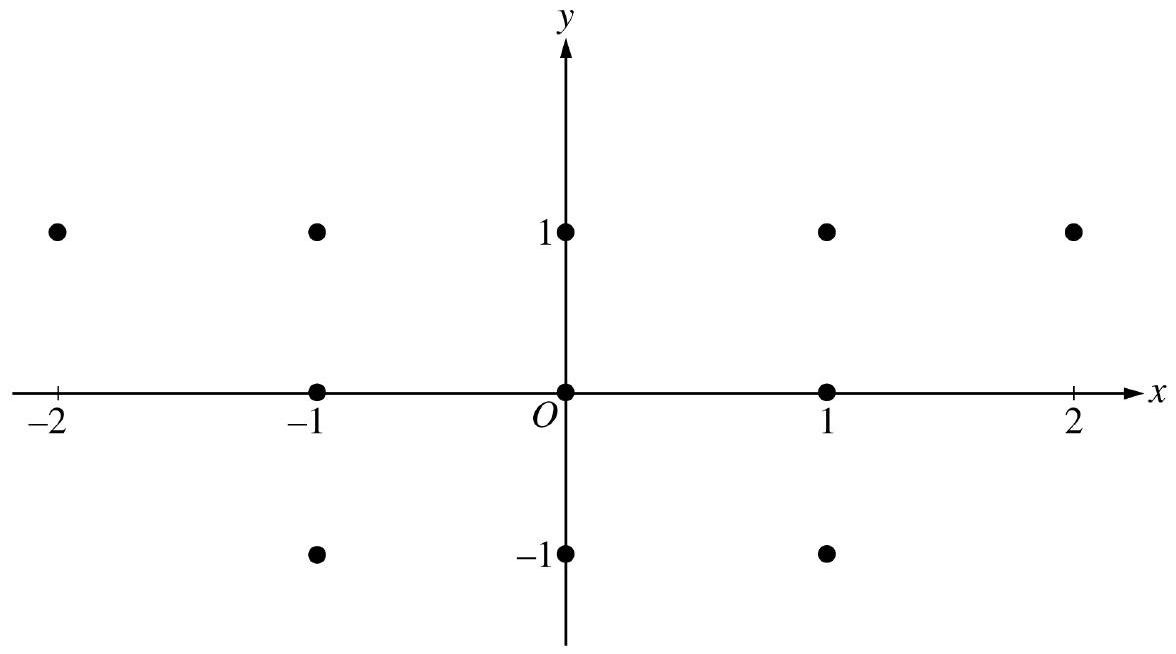
\includegraphics[width=0.6\linewidth]{figures/bc-2000_fig3.jpg}
\end{center}
\part Use the slope field for the given differential equation to explain why a solution could not have the graph shown below.\\
\begin{center}
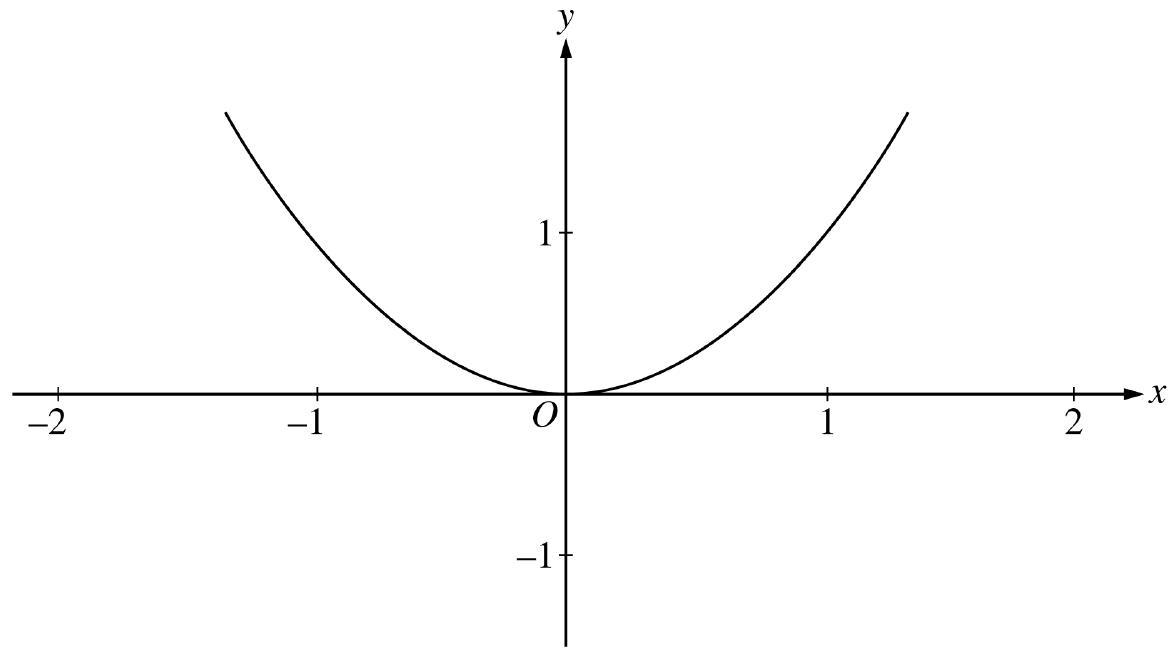
\includegraphics[width=0.6\linewidth]{figures/bc-2000_fig4.jpg}
\end{center}
\part Find the particular solution $y=f(x)$ to the given differential equation with the initial condition $f(0)=-1$.
\part Find the range of the solution found in part (c).
\end{parts}

\end{questions}

\section*{2001 AP Calculus BC}

\begin{questions}

\question
% Q1 | 2001 Calculus BC | Part A | Calculator Active
An object moving along a curve in the $x y$-plane has position $(x(t), y(t))$ at time $t$ with
\[\frac{d x}{d t}=\cos \left(t^{3}\right) \text { and } \frac{d y}{d t}=3 \sin \left(t^{2}\right)\]

for $0 \leq t \leq 3$. At time $t=2$, the object is at position (4,5).\\
\begin{parts}
\part Write an equation for the line tangent to the curve at $(4,5)$.
\part Find the speed of the object at time $t=2$.
\part Find the total distance traveled by the object over the time interval $0 \leq t \leq 1$.
\part Find the position of the object at time $t=3$.
\end{parts}
\begin{solution}
\begin{parts}
\part $\frac{d y}{d x}=\frac{3 \sin \left(t^{2}\right)}{\cos \left(t^{3}\right)}$

\[\begin{aligned}
& \left.\frac{d y}{d x}\right|_{t=2}=\frac{3 \sin \left(2^{2}\right)}{\cos \left(2^{3}\right)}=15.604 \\
& y-5=15.604(x-4)
\end{aligned}\]
\part Speed $=\sqrt{\cos ^{2}(8)+9 \sin ^{2}(4)}=2.275$
\part Distance $=\int_{0}^{1} \sqrt{\cos ^{2}\left(t^{3}\right)+9 \sin ^{2}\left(t^{2}\right)} d t$

\[=1.458\]
\part $x(3)=4+\int_{2}^{3} \cos \left(t^{3}\right) d t=3.953$ or 3.954

\[y(3)=5+\int_{2}^{3} 3 \sin \left(t^{2}\right) d t=4.906\]
\end{parts}
\par\medskip
\textbf{Rubric:}\par
\begin{parts}
\part 1 : tangent line
\part 1 : answer
\part $3:\left\{\begin{aligned}
2: & \text { distance integral } \\
& <-1>\text { each integrand error } \\
& <-1>\text { error in limits } \\
1: & \text { answer }
\end{aligned}\right.$
\part $4:\left\{\begin{array}{l}
1: \text { definite integral for } x \\
1: \text { answer for } x(3) \\
1: \text { definite integral for } y \\
1: \text { answer for } y(3)
\end{array}\right.$
\end{parts}
\end{solution}

\question
% Q2 | 2001 Calculus BC | Part A | Calculator Active
\begin{center}
\begin{tabular}{|c|c|}
\hline
\begin{tabular}{c}
$t$ \\
(days) \\
\end{tabular} & \begin{tabular}{c}
$W(t)$ \\
$\left({ }^{\circ} \mathrm{C}\right)$ \\
\end{tabular} \\
\hline\hline
0 & 20 \\
3 & 31 \\
6 & 28 \\
9 & 24 \\
12 & 22 \\
15 & 21 \\
\hline
\end{tabular}
\end{center}
The temperature, in degrees Celsius ( ${ }^{\circ} \mathrm{C}$ ), of the water in a pond is a differentiable function $W$ of time $t$. The table above shows the water temperature as recorded every 3 days over a 15-day period.\\
\begin{parts}
\part Use data from the table to find an approximation for $W^{\prime}(12)$. Show the computations that lead to your answer. Indicate units of measure.
\part Approximate the average temperature, in degrees Celsius, of the water over the time interval $0 \leq t \leq 15$ days by using a trapezoidal approximation with subintervals of length $\Delta t=3$ days.
\part A student proposes the function $P$, given by $P(t)=20+10 t e^{(-t / 3)}$, as a model for the temperature of the water in the pond at time $t$, where $t$ is measured in days and $P(t)$ is measured in degrees Celsius. Find $P^{\prime}(12)$. Using appropriate units, explain the meaning of your answer in terms of water temperature.
\part Use the function $P$ defined in part (c) to find the average value, in degrees Celsius, of $P(t)$ over the time interval $0 \leq t \leq 15$ days.
\end{parts}
\begin{solution}
\begin{parts}
\part Difference quotient; e.g.

\begin{align*}& W^{\prime}(12) \approx \frac{W(15)-W(12)}{15-12}=-\frac{1}{3}{ }^{\circ} \mathrm{C} / \text { day or } \\
& W^{\prime}(12) \approx \frac{W(12)-W(9)}{12-9}=-\frac{2}{3}{ }^{\circ} \mathrm{C} / \text { day or } \\
& W^{\prime}(12) \approx \frac{W(15)-W(9)}{15-9}=-\frac{1}{2}{ }^{\circ} \mathrm{C} / \text { day }\end{align*}
\part $\frac{3}{2}(20+2(31)+2(28)+2(24)+2(22)+21)=376.5$ Average temperature $\approx \frac{1}{15}(376.5)=25.1^{\circ} \mathrm{C}$
\part $P^{\prime}(12)=10 e^{-t / 3}-\left.\frac{10}{3} t e^{-t / 3}\right|_{t=12}$

\[=-30 e^{-4}=-0.549^{\circ} \mathrm{C} / \text { day }\]

This means that the temperature is decreasing at the rate of $0.549{ }^{\circ} \mathrm{C} /$ day when $t=12$ days.
\part $\frac{1}{15} \int_{0}^{15}\left(20+10 t e^{-t / 3}\right) d t=25.757^{\circ} \mathrm{C}$
\end{parts}
\par\medskip
\textbf{Rubric:}\par
\begin{parts}
\part $1: P^{\prime}(12) \text { (with or without units) }$
\end{parts}
\end{solution}

\question
% Q3 | 2001 Calculus BC | Part A | Calculator Active
\begin{center}
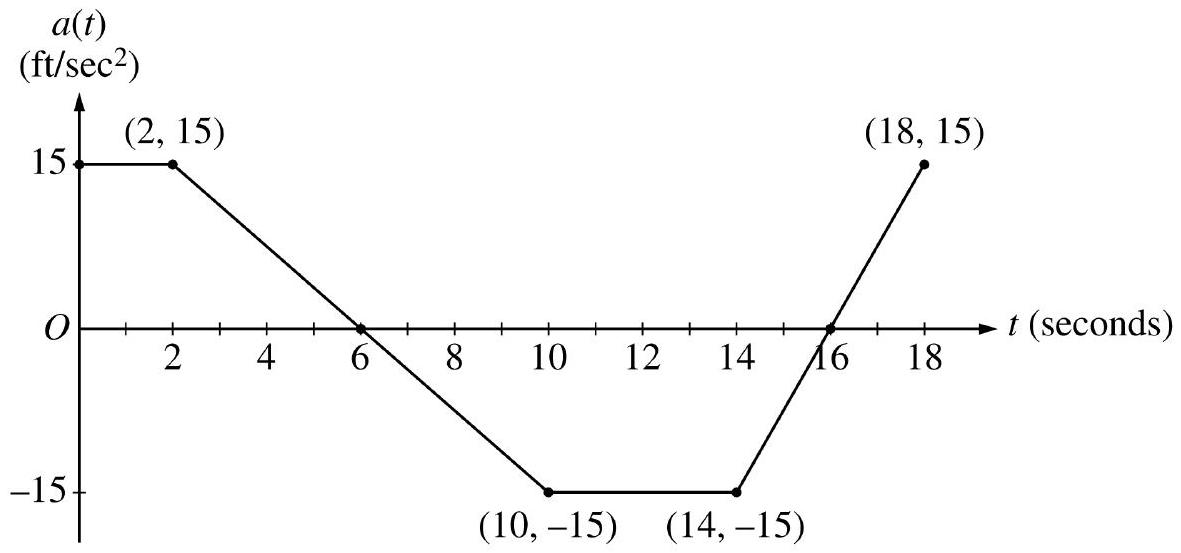
\includegraphics[width=0.6\linewidth]{figures/bc-2001_fig1.jpg}
\end{center}
A car is traveling on a straight road with velocity $55 \mathrm{ft} / \mathrm{sec}$ at time $t=0$. For $0 \leq t \leq 18$ seconds, the car's acceleration $a(t)$, in $\mathrm{ft} / \mathrm{sec}^{2}$, is the piecewise linear function defined by the graph above.\\
\begin{parts}
\part Is the velocity of the car increasing at $t=2$ seconds? Why or why not?
\part At what time in the interval $0 \leq t \leq 18$, other than $t=0$, is the velocity of the car $55 \mathrm{ft} / \mathrm{sec}$ ? Why?
\part On the time interval $0 \leq t \leq 18$, what is the car's absolute maximum velocity, in $\mathrm{ft} / \mathrm{sec}$, and at what time does it occur? Justify your answer.
\part At what times in the interval $0 \leq t \leq 18$, if any, is the car's velocity equal to zero? Justify your answer.
\end{parts}
\begin{solution}
\begin{parts}
\part Since $v^{\prime}(2)=a(2)$ and $a(2)=15>0$, the velocity is increasing at $t=2$.
\part At time $t=12$ because

\[v(12)-v(0)=\int_{0}^{12} a(t) d t=0\]
\part The absolute maximum velocity is $115 \mathrm{ft} / \mathrm{sec}$ at $t=6$.\\
The absolute maximum must occur at $t=6$ or at an endpoint.

\begin{align*}& v(6)=55+\int_{0}^{6} a(t) d t \\
& \quad=55+2(15)+\frac{1}{2}(4)(15)=115>v(0) \\
& \int_{6}^{18} a(t) d t<0 \text { so } v(18)<v(6)\end{align*}
\part The car's velocity is never equal to 0 . The absolute minimum occurs at $t=16$ where

\[v(16)=115+\int_{6}^{16} a(t) d t=115-105=10>0\]
\end{parts}
\par\medskip
\textbf{Rubric:}\par
\begin{parts}
\part 1 : answer and reason
\part $2:\left\{\begin{array}{l}
1: t=12 \\
1: \text { reason }
\end{array}\right.$
\part 1: t=6
\end{parts}
\end{solution}

\question
% Q4 | 2001 Calculus BC | Part B | Calculator Prohibited
Let $h$ be a function defined for all $x \neq 0$ such that $h(4)=-3$ and the derivative of $h$ is given by $h^{\prime}(x)=\frac{x^{2}-2}{x}$ for all $x \neq 0$.\\
\begin{parts}
\part Find all values of $x$ for which the graph of $h$ has a horizontal tangent, and determine whether $h$ has a local maximum, a local minimum, or neither at each of these values. Justify your answers.
\part On what intervals, if any, is the graph of $h$ concave up? Justify your answer.
\part Write an equation for the line tangent to the graph of $h$ at $x=4$.
\part Does the line tangent to the graph of $h$ at $x=4$ lie above or below the graph of $h$ for $x>4$ ? Why?
\end{parts}
\begin{solution}
\begin{parts}
\part $\quad h^{\prime}(x)=0$ at $x= \pm \sqrt{2}$\\
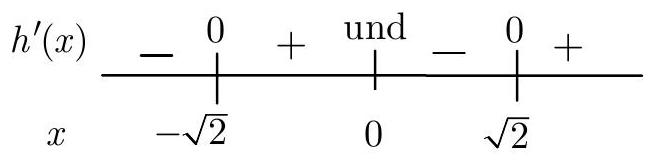
\includegraphics[width=0.6\linewidth]{figures/sg-bc-2001_fig2.jpg}

Local minima at $x=-\sqrt{2}$ and at $x=\sqrt{2}$
\part $h^{\prime \prime}(x)=1+\frac{2}{x^{2}}>0$ for all $x \neq 0$. Therefore, the graph of $h$ is concave up for all $x \neq 0$.
\part $\quad h^{\prime}(4)=\frac{16-2}{4}=\frac{7}{2}$

\[y+3=\frac{7}{2}(x-4)\]
\part The tangent line is below the graph because the graph of $h$ is concave up for $x>4$.
\end{parts}
\par\medskip
\textbf{Rubric:}\par
\begin{parts}
\part $4:\left\{\begin{aligned}
1: & x= \pm \sqrt{2} \\
1: & \text { analysis } \\
2: & \text { conclusions } \\
& <-1>\text { not dealing with } \\
& \quad \text { discontinuity at } 0
\end{aligned}\right.$
\part $3:\left\{\begin{array}{l}1: h^{\prime \prime}(x) \\ 1: h^{\prime \prime}(x)>0 \\ 1: \text { answer }\end{array}\right.$
\part 1 : tangent line equation
\part 1 : answer with reason
\end{parts}
\end{solution}

\question
% Q5 | 2001 Calculus BC | Part B | Calculator Prohibited
Let $f$ be the function satisfying $f^{\prime}(x)=-3 x f(x)$, for all real numbers $x$, with $f(1)=4$ and $\lim _{x \rightarrow \infty} f(x)=0$.\\
\begin{parts}
\part Evaluate $\int_{1}^{\infty}-3 x f(x) d x$. Show the work that leads to your answer.
\part Use Euler's method, starting at $x=1$ with a step size of 0.5 , to approximate $f(2)$.
\part Write an expression for $y=f(x)$ by solving the differential equation $\frac{d y}{d x}=-3 x y$ with the initial condition $f(1)=4$.
\end{parts}
\begin{solution}
\begin{parts}
\part $\int_{1}^{\infty}-3 x f(x) d x$\\
$=\int_{1}^{\infty} f^{\prime}(x) d x=\lim _{b \rightarrow \infty} \int_{1}^{b} f^{\prime}(x) d x=\left.\lim _{b \rightarrow \infty} f(x)\right|_{1} ^{b}$\\
$=\lim _{b \rightarrow \infty} f(b)-f(1)=0-4=-4$
\part $f(1.5) \approx f(1)+f^{\prime}(1)(0.5)$\\
$=4-3(1)(4)(0.5)=-2$\\
$f(2) \approx-2+f^{\prime}(1.5)(0.5)$

\[\approx-2-3(1.5)(-2)(0.5)=2.5\]
\part $\frac{1}{y} d y=-3 x d x$\\
$\ln y=-\frac{3}{2} x^{2}+k$\\
$y=C e^{-3 / 2 x^{2}}$\\
$4=C e^{-3 / 2} ; C=4 e^{3 / 2}$\\
$y=4 e^{3 / 2} e^{-3 / 2 x^{2}}$
\end{parts}
\par\medskip
\textbf{Rubric:}\par
\begin{parts}
\part $2:\left\{\begin{array}{l}1: \text { use of FTC } \\ 1: \text { answer from limiting process }\end{array}\right.$
\part $2:\left\{\begin{aligned} 1: & \text { Euler's method equations or } \\ & \text { equivalent table } \\ 1: & \text { Euler approximation to } f(2) \\ & \text { (not eligible without first point) }\end{aligned}\right.$
\part $5:\left\{\begin{array}{l}1: \text { separates variables } \\ 1: \text { antiderivatives } \\ 1: \text { constant of integration } \\ 1: \text { uses initial condition } f(1)=4 \\ 1: \text { solves for } y\end{array}\right.$
\part Note: $\max 2 / 5[1-1-0-0-0]$ if no constant of integration
\part Note: 0/5 if no separation of variables
\end{parts}
\end{solution}

\question
% Q6 | 2001 Calculus BC | Part B | Calculator Prohibited
A function $f$ is defined by
\[f(x)=\frac{1}{3}+\frac{2}{3^{2}} x+\frac{3}{3^{3}} x^{2}+\cdots+\frac{n+1}{3^{n+1}} x^{n}+\cdots\]

for all $x$ in the interval of convergence of the given power series.\\
\begin{parts}
\part Find the interval of convergence for this power series. Show the work that leads to your answer.
\part Find $\lim _{x \rightarrow 0} \frac{f(x)-\frac{1}{3}}{x}$.
\part Write the first three nonzero terms and the general term for an infinite series that represents $\int_{0}^{1} f(x) d x$.
\part Find the sum of the series determined in part (c).
\end{parts}
\begin{solution}
\begin{parts}
\part $\lim _{n \rightarrow \infty}\left|\frac{\frac{(n+2) x^{n+1}}{3^{n+2}}}{\frac{(n+1) x^{n}}{3^{n+1}}}\right|=\lim _{n \rightarrow \infty}\left|\frac{(n+2)}{(n+1)} \frac{x}{3}\right|=\left|\frac{x}{3}\right|<1$

At $x=-3$, the series is $\sum_{n=0}^{\infty}(-1)^{n} \frac{n+1}{3}$, which diverges.\\
At $x=3$, the series is $\sum_{n=0}^{\infty} \frac{n+1}{3}$, which diverges.\\
Therefore, the interval of convergence is $-3<x<3$.
\part $\lim _{x \rightarrow 0} \frac{f(x)-\frac{1}{3}}{x}=\lim _{x \rightarrow 0}\left(\frac{2}{3^{2}}+\frac{3}{3^{3}} x+\frac{4}{3^{4}} x^{2}+\cdots\right)=\frac{2}{9}$
\part $\quad \int_{0}^{1} f(x) d x=\int_{0}^{1}\left(\frac{1}{3}+\frac{2}{3^{2}} x+\frac{3}{3^{3}} x^{2}+\cdots+\frac{n+1}{3^{n+1}} x^{n}+\cdots\right) d x$

\[\begin{aligned}
& =\left.\left(\frac{1}{3} x+\frac{1}{3^{2}} x^{2}+\frac{1}{3^{3}} x^{3}+\cdots+\frac{1}{3^{n+1}} x^{n+1}+\cdots\right)\right|_{x=0} ^{x=1} \\
& =\frac{1}{3}+\frac{1}{3^{2}}+\frac{1}{3^{3}}+\cdots+\frac{1}{3^{n+1}}+\cdots
\end{aligned}\]
\part The series representing $\int_{0}^{1} f(x) d x$ is a geometric series.

Therefore, $\int_{0}^{1} f(x) d x=\frac{\frac{1}{3}}{1-\frac{1}{3}}=\frac{1}{2}$.
\end{parts}
\par\medskip
\textbf{Rubric:}\par
\begin{parts}
\part $4:\left\{\begin{array}{l}1: \text { sets up ratio test } \\ 1: \text { computes limit } \\ 1: \text { conclusion of ratio test } \\ 1: \text { endpoint conclusion }\end{array}\right.$
\part 1 : answer
\part $3:\left\{\begin{aligned} 1: & \text { antidifferentiation } \\ & \text { of series } \\ 1: & \text { first three terms for } \\ & \text { definite integral series } \\ 1: & \text { general term }\end{aligned}\right.$
\part 1 : answer
\end{parts}
\end{solution}

\end{questions}

\section*{2002 AP Calculus BC}

\begin{questions}

\question
% Q1 | 2002 Calculus BC | Part A | Calculator Active
Let $f$ and $g$ be the functions given by $f(x)=e^{x}$ and $g(x)=\ln x$.\\
\begin{parts}
\part Find the area of the region enclosed by the graphs of $f$ and $g$ between $x=\frac{1}{2}$ and $x=1$.
\part Find the volume of the solid generated when the region enclosed by the graphs of $f$ and $g$ between $x=\frac{1}{2}$ and $x=1$ is revolved about the line $y=4$.
\part Let $h$ be the function given by $h(x)=f(x)-g(x)$. Find the absolute minimum value of $h(x)$ on the closed interval $\frac{1}{2} \leq x \leq 1$, and find the absolute maximum value of $h(x)$ on the closed interval $\frac{1}{2} \leq x \leq 1$. Show the analysis that leads to your answers.
\end{parts}
\begin{solution}
\begin{parts}
\part Area $=\int_{1 / 2}^{1}\left(e^{x}-\ln x\right) d x=1.222$ or 1.223
\part Volume $=\pi \int_{1 / 2}^{1}\left((4-\ln x)^{2}-\left(4-e^{x}\right)^{2}\right) d x$

\[=7.515 \pi \text { or } 23.609\]
\part $h^{\prime}(x)=f^{\prime}(x)-g^{\prime}(x)=e^{x}-\frac{1}{x}=0 x=0.567143$

Absolute minimum value and absolute maximum value occur at the critical point or at the endpoints.

\begin{align*}& h(0.567143)=2.330 \\
& h(0.5)=2.3418 \\
& h(1)=2.718\end{align*}

The absolute minimum is 2.330 .\\
The absolute maximum is 2.718 .
\end{parts}
\par\medskip
\textbf{Rubric:}\par
\begin{parts}
\part Note: Errors in computation come off the third point.
\end{parts}
\end{solution}

\question
% Q2 | 2002 Calculus BC | Part A | Calculator Active
The rate at which people enter an amusement park on a given day is modeled by the function $E$ defined by
\[E(t)=\frac{15600}{\left(t^{2}-24 t+160\right)}\]

The rate at which people leave the same amusement park on the same day is modeled by the function $L$ defined by

\[L(t)=\frac{9890}{\left(t^{2}-38 t+370\right)}\]

Both $E(t)$ and $L(t)$ are measured in people per hour and time $t$ is measured in hours after midnight. These functions are valid for $9 \leq t \leq 23$, the hours during which the park is open. At time $t=9$, there are no people in the park.\\
\begin{parts}
\part How many people have entered the park by 5:00 P.M. ( $t=17$ )? Round your answer to the nearest whole number.
\part The price of admission to the park is $\$ 15$ until 5:00 P.M. ( $t=17$ ). After 5:00 P.M., the price of admission to the park is $\$ 11$. How many dollars are collected from admissions to the park on the given day? Round your answer to the nearest whole number.
\part Let $H(t)=\int_{9}^{t}(E(x)-L(x)) d x$ for $9 \leq t \leq 23$. The value of $H(17)$ to the nearest whole number is 3725 . Find the value of $H^{\prime}(17)$, and explain the meaning of $H(17)$ and $H^{\prime}(17)$ in the context of the amusement park.
\part At what time $t$, for $9 \leq t \leq 23$, does the model predict that the number of people in the park is a maximum?
\end{parts}
\begin{solution}
\begin{parts}
\part $\int_{9}^{17} E(t) d t=6004.270$

6004 people entered the park by 5 pm .
\part $15 \int_{9}^{17} E(t) d t+11 \int_{17}^{23} E(t) d t=104048.165$

The amount collected was $\$ 104,048$.\\
or\\
$\int_{17}^{23} E(t) d t=1271.283$\\
1271 people entered the park between 5 pm and 11 pm , so the amount collected was\\
$\$ 15 \cdot(6004)+\$ 11 \cdot(1271)=\$ 104,041$.
\part $H^{\prime}(17)=E(17)-L(17)=-380.281$

There were 3725 people in the park at $t=17$.\\
The number of people in the park was decreasing at the rate of approximately 380 people/hr at time $t=17$.
\part $H^{\prime}(t)=E(t)-L(t)=0$
\end{parts}
\par\medskip
\textbf{Rubric:}\par
\[\begin{aligned}
& 3\left\{\begin{array}{l}
1: \text { limits } \\
1: \text { integrand } \\
1: \text { answer }
\end{array}\right. \\
& 1: \text { setup } \\
& 3 \begin{cases}1: & \text { value of } H^{\prime}(17) \\
2: & \text { meanings } \\
1: \text { meaning of } H(17) \\
1: \text { meaning of } H^{\prime}(17) \\
<-1>\text { if no reference to } t=17\end{cases}
\end{aligned}\]

$t=15.794$ or 15.795
\end{solution}

\question
% Q3 | 2002 Calculus BC | Part A | Calculator Active
\begin{center}
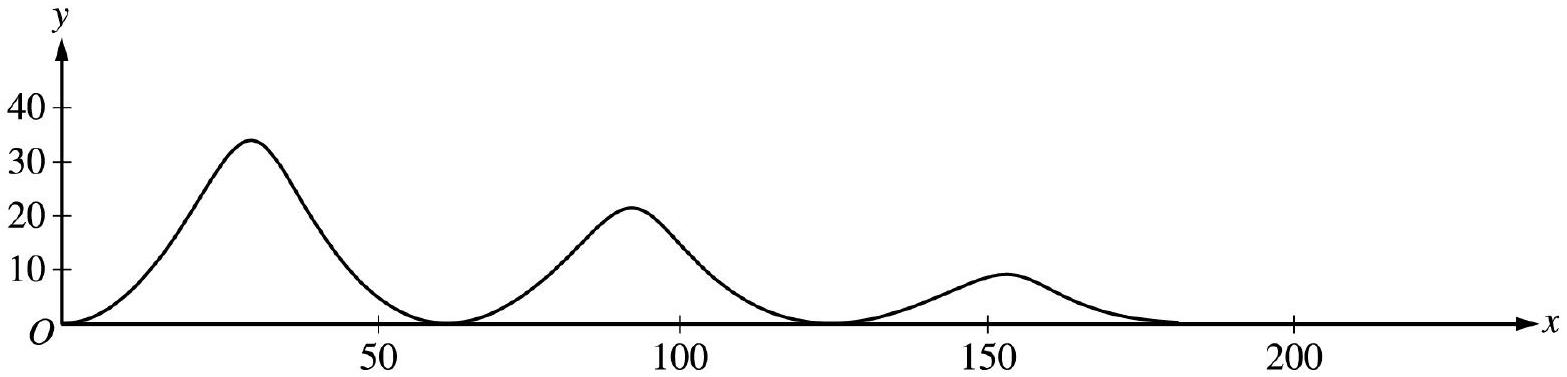
\includegraphics[width=0.6\linewidth]{figures/bc-2002_fig1.jpg}
\end{center}
The figure above shows the path traveled by a roller coaster car over the time interval $0 \leq t \leq 18$ seconds. The position of the car at time $t$ seconds can be modeled parametrically by

\begin{align*}& x(t)=10 t+4 \sin t \\
& y(t)=(20-t)(1-\cos t),\end{align*}

where $x$ and $y$ are measured in meters. The derivatives of these functions are given by

\begin{align*}& x^{\prime}(t)=10+4 \cos t \\
& y^{\prime}(t)=(20-t) \sin t+\cos t-1\end{align*}
\begin{parts}
\part Find the slope of the path at time $t=2$. Show the computations that lead to your answer.
\part Find the acceleration vector of the car at the time when the car's horizontal position is $x=140$.
\part Find the time $t$ at which the car is at its maximum height, and find the speed, in $\mathrm{m} / \mathrm{sec}$, of the car at this time.
\part For $0<t<18$, there are two times at which the car is at ground level ( $y=0$ ). Find these two times and write an expression that gives the average speed, in $\mathrm{m} / \mathrm{sec}$, of the car between these two times. Do not evaluate the expression.
\end{parts}
\begin{solution}
\begin{parts}
\part Slope $=\left.\frac{d y}{d x}\right|_{t=2}=\frac{y^{\prime}(2)}{x^{\prime}(2)}=\frac{18 \sin 2+\cos 2-1}{10+4 \cos 2}$

\[=1.793 \text { or } 1.794\]
\part $\quad x(t)=10 t+4 \sin t=140 ; t_{0}=13.647083$\\
$x^{\prime \prime}\left(t_{0}\right)=-3.529, y^{\prime \prime}\left(t_{0}\right)=1.225$ or 1.226\\
Acceleration vector is $<-3.529,1.225>$

\[\text { or }<-3.529,1.226>\]
\part $y^{\prime}(t)=(20-t) \sin t+\cos t-1=0$\\
$t_{1}=3.023$ or 3.024 at maximum height

\[\begin{aligned}
\text { Speed } & =\sqrt{\left(x^{\prime}\left(t_{1}\right)\right)^{2}+\left(y^{\prime}\left(t_{1}\right)\right)^{2}}=\left|x^{\prime}\left(t_{1}\right)\right| \\
& =6.027 \text { or } 6.028
\end{aligned}\]
\part $y(t)=0$ when $t=2 \pi$ and $t=4 \pi$

Average speed $=\frac{1}{2 \pi} \int_{2 \pi}^{4 \pi} \sqrt{\left(x^{\prime}(t)\right)^{2}+\left(y^{\prime}(t)\right)^{2}} d t$\\
$=\frac{1}{2 \pi} \int_{2 \pi}^{4 \pi} \sqrt{(10+4 \cos t)^{2}+((20-t) \sin t+\cos t-1)^{2}} d t$
\end{parts}
\par\medskip
\textbf{Rubric:}\par
\begin{parts}
\part 1 : answer using $\frac{d y}{d x}=\frac{d y}{d t} / \frac{d x}{d t}$
\part $2\left\{\begin{aligned} 1: & \text { identifies acceleration vector } \\ & \text { as derivative of velocity vector } \\ 1: & \text { computes acceleration vector } \\ & \text { when } x=140\end{aligned}\right.$
\part $3\left\{\begin{aligned} 1: & \text { sets } y^{\prime}(t)=0 \\ 1: & \text { selects first } t>0 \\ 1: & \text { speed }\end{aligned}\right.$
\part $3\left\{\begin{array}{l}1: t=2 \pi, t=4 \pi \\ 1: \text { limits and constant } \\ 1: \text { integrand }\end{array}\right.$
\end{parts}
\end{solution}

\question
% Q4 | 2002 Calculus BC | Part B | Calculator Prohibited
\begin{center}
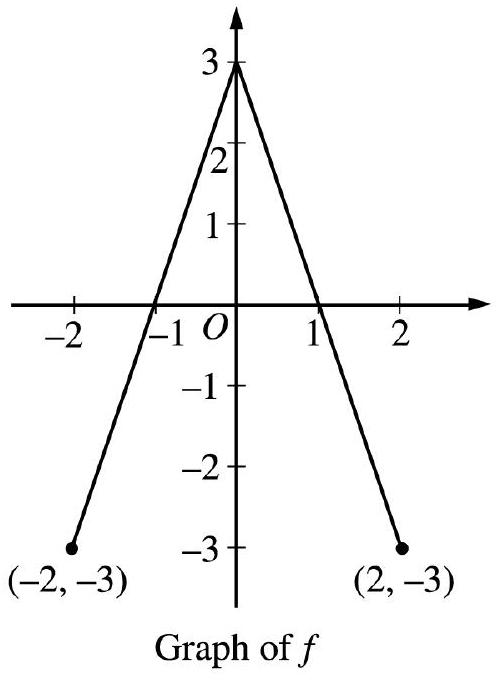
\includegraphics[width=0.6\linewidth]{figures/bc-2002_fig2.jpg}
\end{center}
The graph of the function $f$ shown above consists of two line segments. Let $g$ be the function given by $g(x)=\int_{0}^{x} f(t) d t$.\\
\begin{parts}
\part Find $g(-1), g^{\prime}(-1)$, and $g^{\prime \prime}(-1)$.
\part For what values of $x$ in the open interval $(-2,2)$ is $g$ increasing? Explain your reasoning.
\part For what values of $x$ in the open interval ( $-2,2$ ) is the graph of $g$ concave down? Explain your reasoning.
\part On the axes provided, sketch the graph of $g$ on the closed interval $[-2,2]$.\\
(Note: The axes are provided in the pink test booklet only.)
\end{parts}
\begin{solution}
\begin{parts}
\part $\quad g(-1)=\int_{0}^{-1} f(t) d t=-\int_{-1}^{0} f(t) d t=-\frac{3}{2}$

\begin{align*}& g^{\prime}(-1)=f(-1)=0 \\
& g^{\prime \prime}(-1)=f^{\prime}(-1)=3\end{align*}
\part $g$ is increasing on $-1<x<1$ because $g^{\prime}(x)=f(x)>0$ on this interval.
\part The graph of $g$ is concave down on $0<x<2$ because $g^{\prime \prime}(x)=f^{\prime}(x)<0$ on this interval.\\
or\\
because $g^{\prime}(x)=f(x)$ is decreasing on this interval.\\
(d)\\
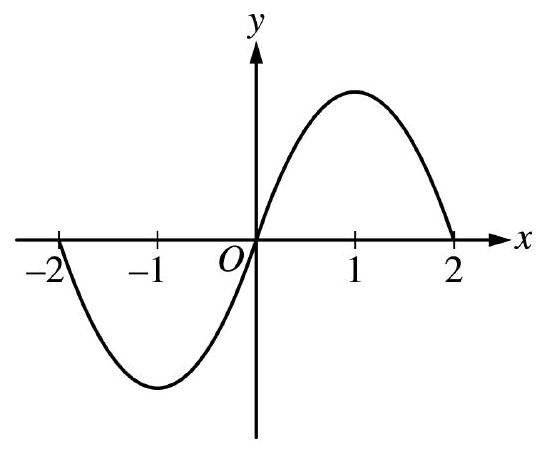
\includegraphics[width=0.6\linewidth]{figures/sg-bc-2002_fig3.jpg}
\end{parts}
\par\medskip
\textbf{Rubric:}\par
\begin{parts}
\part $3 \begin{cases}1: & g(-1) \\ 1: & g^{\prime}(-1) \\ 1: & g^{\prime \prime}(-1)\end{cases}$
\part $2\left\{\begin{array}{l}
1: \text { interval } \\
1: \text { reason }
\end{array}\right.$
\part $2\left\{\begin{array}{l}
1: \text { interval } \\
1: \text { reason }
\end{array}\right.$
\part $2\left\{\begin{aligned}
1: & g(-2)=g(0)=g(2)=0 \\
1: & \text { appropriate increasing/decreasing } \\
& \text { and concavity behavior } \\
& <-1>\text { vertical asymptote }
\end{aligned}\right.$
\end{parts}
\end{solution}

\question
% Q5 | 2002 Calculus BC | Part B | Calculator Prohibited
Consider the differential equation $\frac{d y}{d x}=2 y-4 x$.\\
\begin{parts}
\part The slope field for the given differential equation is provided. Sketch the solution curve that passes through the point $(0,1)$ and sketch the solution curve that passes through the point $(0,-1)$.\\
(Note: Use the slope field provided in the pink test booklet.)\\
\begin{center}
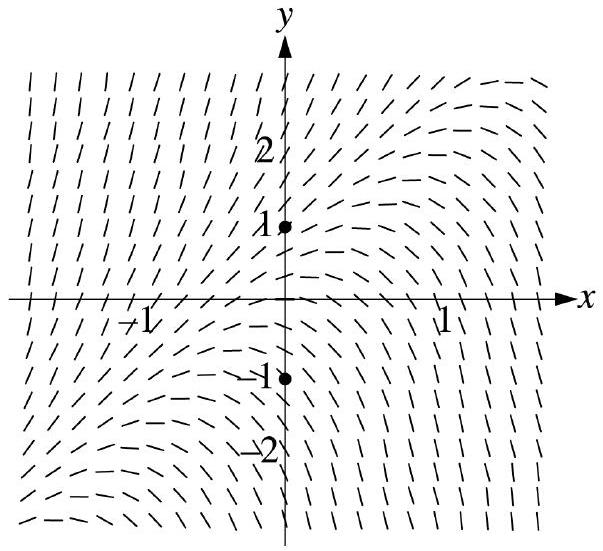
\includegraphics[width=0.6\linewidth]{figures/bc-2002_fig3.jpg}
\end{center}
\part Let $f$ be the function that satisfies the given differential equation with the initial condition $f(0)=1$. Use Euler's method, starting at $x=0$ with a step size of 0.1 , to approximate $f(0.2)$. Show the work that leads to your answer.
\part Find the value of $b$ for which $y=2 x+b$ is a solution to the given differential equation. Justify your answer.
\part Let $g$ be the function that satisfies the given differential equation with the initial condition $g(0)=0$. Does the graph of $g$ have a local extremum at the point $(0,0)$ ? If so, is the point a local maximum or a local minimum? Justify your answer.
\end{parts}
\begin{solution}
(a)\\
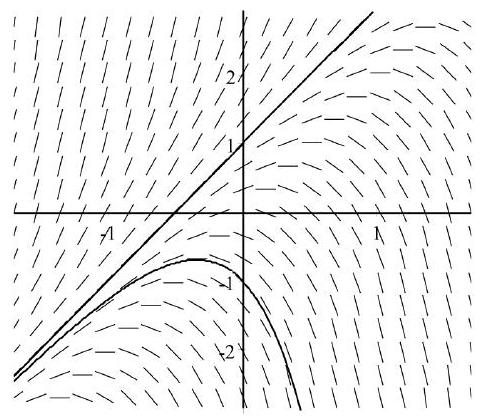
\includegraphics[width=0.6\linewidth]{figures/sg-bc-2002_fig4.jpg}\\
\begin{parts}
\part $f(0.1) \approx f(0)+f^{\prime}(0)(0.1)$

\begin{align*}& =1+(2-0)(0.1)=1.2 \\
f(0.2) & \approx f(0.1)+f^{\prime}(0.1)(0.1) \\
& \approx 1.2+(2.4-0.4)(0.1)=1.4\end{align*}
\part Substitute $y=2 x+b$ in the DE:\\
$2=2(2 x+b)-4 x=2 b$, so $b=1$\\
OR\\
Guess $b=1, y=2 x+1$\\
Verify: $2 y-4 x=(4 x+2)-4 x=2=\frac{d y}{d x}$.
\part $g$ has local maximum at $(0,0)$.\\
$g^{\prime}(0)=\left.\frac{d y}{d x}\right|_{(0,0)}=2(0)-4(0)=0$, and\\
$g^{\prime \prime}(x)=\frac{d^{2} y}{d x^{2}}=2 \frac{d y}{d x}-4$, so\\
$g^{\prime \prime}(0)=2 g^{\prime}(0)-4=-4<0$.
\end{parts}
\par\medskip
\textbf{Rubric:}\par
\begin{parts}
\part $2 \begin{cases}1: & \text { solution curve through }(0,1) \\ 1: & \text { solution curve through }(0,-1)\end{cases}$
\part 1: Euler's method equations or equivalent table applied to (at least) two iterations
\part 1 : Euler approximation to $f(0.2)$ (not eligible without first point)
\part $2\left\{\begin{array}{l}1: \text { uses } \frac{d}{d x}(2 x+b)=2 \text { in DE } \\ 1: \quad b=1\end{array}\right.$
\part $3 \begin{cases}1: & g^{\prime}(0)=0 \\ 1: & \text { shows } g^{\prime \prime}(0)=-4 \\ 1: & \text { conclusion }\end{cases}$
\end{parts}
\end{solution}

\question
% Q6 | 2002 Calculus BC | Part B | Calculator Prohibited
The Maclaurin series for the function $f$ is given by

\[f(x)=\sum_{n=0}^{\infty} \frac{(2 x)^{n+1}}{n+1}=2 x+\frac{4 x^{2}}{2}+\frac{8 x^{3}}{3}+\frac{16 x^{4}}{4}+\cdots+\frac{(2 x)^{n+1}}{n+1}+\cdots\]

on its interval of convergence.\\
\begin{parts}
\part Find the interval of convergence of the Maclaurin series for $f$. Justify your answer.
\part Find the first four terms and the general term for the Maclaurin series for $f^{\prime}(x)$.
\part Use the Maclaurin series you found in part (b) to find the value of $f^{\prime}\left(-\frac{1}{3}\right)$.
\end{parts}
\begin{solution}
\begin{parts}
\part $\lim _{n \rightarrow \infty}\left|\frac{\frac{(2 x)^{n+2}}{n+2}}{\frac{(2 x)^{n+1}}{n+1}}\right|=\lim _{n \rightarrow \infty}\left|\frac{(n+1)}{(n+2)} 2 x\right|=|2 x|$\\
$|2 x|<1$ for $-\frac{1}{2}<x<\frac{1}{2}$\\
At $x=\frac{1}{2}$, the series is $\sum_{n=0}^{\infty} \frac{1}{n+1}$ which diverges since this is the harmonic series.\\
At $x=-\frac{1}{2}$, the series is $\sum_{n=0}^{\infty}(-1)^{n+1} \frac{1}{n+1}$ which converges by the Alternating Series Test.

Hence, the interval of convergence is $-\frac{1}{2} \leq x<\frac{1}{2}$.
\part $f^{\prime}(x)=2+4 x+8 x^{2}+16 x^{3}+\ldots+2(2 x)^{n}+\ldots$
\part The series in (b) is a geometric series.

\[\begin{aligned}
f^{\prime}\left(-\frac{1}{3}\right) & =2+4\left(-\frac{1}{3}\right)+8\left(-\frac{1}{3}\right)^{2}+\ldots+2\left(2 \cdot\left(-\frac{1}{3}\right)\right)^{n}+\ldots \\
& =2-\frac{4}{3}+\frac{8}{9}-\frac{16}{27}+\ldots+2\left(-\frac{2}{3}\right)^{n}+\ldots \\
& =\frac{2}{1+\frac{2}{3}}=\frac{6}{5} \\
f^{\prime}(x) & =\frac{2}{1-2 x} \text { for }-\frac{1}{2}<x<\frac{1}{2} . \text { Therefore, } \\
f^{\prime}\left(-\frac{1}{3}\right) & =\frac{2}{1+\frac{2}{3}}=\frac{6}{5}
\end{aligned}\]
\end{parts}
\par\medskip
\textbf{Rubric:}\par
\begin{parts}
\part 1 : sets up ratio
\part 1 : computes limit of ratio
\part 1: identifies interior of interval of convergence
\part 2 : analysis/conclusion at endpoints
\part 1 : right endpoint
\part 1: left endpoint
\part $2 \begin{cases}1: & \text { first } 4 \text { terms } \\ 1: & \text { general term }\end{cases}$
\part $2\left\{\begin{aligned}
1: & \text { substitutes } x=-\frac{1}{3} \text { into infinite } \\
& \text { series from (b) or expresses series } \\
& \text { from (b) in closed form } \\
1: & \text { answer for student's series }
\end{aligned}\right.$
\end{parts}
\end{solution}

\end{questions}

\section*{2002 AP Calculus BC Form B}

\begin{questions}

\question
% Q1 | 2002 Calculus BC Form B | Part A | Calculator Active
A particle moves in the $x y$-plane so that its position at any time $t$, for $-\pi \leq t \leq \pi$, is given by $x(t)=\sin (3 t)$ and $y(t)=2 t$.\\
\begin{parts}
\part Sketch the path of the particle in the $x y$-plane provided. Indicate the direction of motion along the path.\\
\begin{center}
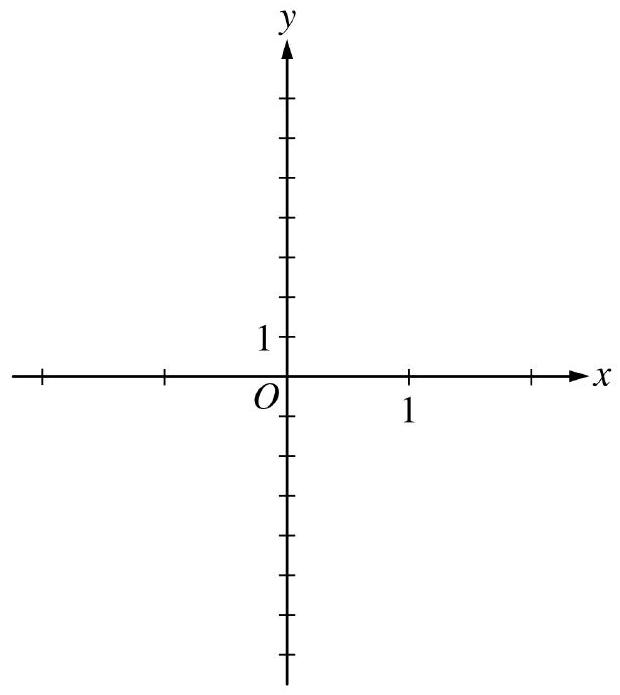
\includegraphics[width=0.6\linewidth]{figures/bc-2002-form-b_fig1.jpg}
\end{center}
\part Find the range of $x(t)$ and the range of $y(t)$.
\part Find the smallest positive value of $t$ for which the $x$-coordinate of the particle is a local maximum. What is the speed of the particle at this time?
\part Is the distance traveled by the particle from $t=-\pi$ to $t=\pi$ greater than $5 \pi$ ? Justify your answer.
\end{parts}
\begin{solution}
(a)\\
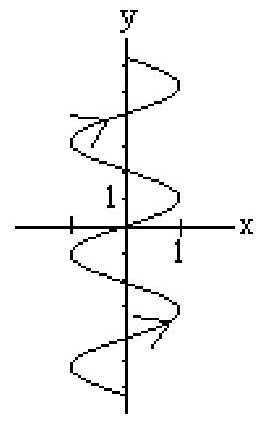
\includegraphics[width=0.6\linewidth]{figures/sg-bc-2002-form-b_fig1.jpg}\\
\begin{parts}
\part $-1 \leq x(t) \leq 1$\\
$-2 \pi \leq y(t) \leq 2 \pi$
\part $x^{\prime}(t)=3 \cos 3 t=0$

\[\begin{aligned}
3 t & =\frac{\pi}{2} ; t=\frac{\pi}{6} \\
\text { Speed } & =\sqrt{9 \cos ^{2}(3 t)+4} \\
\text { At } t & =\frac{\pi}{6} \\
\text { Speed } & =\sqrt{9 \cos ^{2}\left(\frac{\pi}{2}\right)+4}=2
\end{aligned}\]
\part Distance $=\int_{-\pi}^{\pi} \sqrt{9 \cos ^{2}(3 t)+4} d t$

\[=17.973>5 \pi\]
\end{parts}
\par\medskip
\textbf{Rubric:}\par
\begin{parts}
\part $1: x^{\prime}(t)=3 \text { cos } 3 t=0$
\end{parts}
\end{solution}

\question
% Q2 | 2002 Calculus BC Form B | Part A | Calculator Active
The number of gallons, $P(t)$, of a pollutant in a lake changes at the rate $P^{\prime}(t)=1-3 e^{-0.2 \sqrt{t}}$ gallons per day, where $t$ is measured in days. There are 50 gallons of the pollutant in the lake at time $t=0$. The lake is considered to be safe when it contains 40 gallons or less of pollutant.\\
\begin{parts}
\part Is the amount of pollutant increasing at time $t=9$ ? Why or why not?
\part For what value of $t$ will the number of gallons of pollutant be at its minimum? Justify your answer.
\part Is the lake safe when the number of gallons of pollutant is at its minimum? Justify your answer.
\part An investigator uses the tangent line approximation to $P(t)$ at $t=0$ as a model for the amount of pollutant in the lake. At what time $t$ does this model predict that the lake becomes safe?
\end{parts}
\begin{solution}
\begin{parts}
\part $P^{\prime}(9)=1-3 e^{-0.6}=-0.646<0$\\
so the amount is not increasing at this time.
\part $P^{\prime}(t)=1-3 e^{-0.2 \sqrt{t}}=0$\\
$t=(5 \ln 3)^{2}=30.174$\\
$P^{\prime}(t)$ is negative for $0<t<(5 \ln 3)^{2}$ and positive for $t>(5 \ln 3)^{2}$. Therefore there is a minimum at $t=(5 \ln 3)^{2}$.
\part $\quad P(30.174)=50+\int_{0}^{30.174}\left(1-3 e^{-0.2 \sqrt{t}}\right) d t =35.104<40$, so the lake is safe.
\part $P^{\prime}(0)=1-3=-2$. The lake will become safe when the amount decreases by 10 . A linear model predicts this will happen when $t=5$.
\end{parts}
\par\medskip
\textbf{Rubric:}\par
\begin{parts}
\part 1 : answer with reason
\part $3\left\{\begin{array}{l}1: \text { sets } P^{\prime}(t)=0 \\ 1: \text { solves for } t \\ 1: \text { justification }\end{array}\right.$
\part $3\left\{\begin{aligned} 1: & \text { integrand } \\ 1: & \text { limits } \\ 1: & \text { conclusion with reason } \\ & \text { based on integral of } P^{\prime}(t)\end{aligned}\right.$
\part $2\left\{\begin{array}{l}1: \text { slope of tangent line } \\ 1: \text { answer }\end{array}\right.$
\end{parts}
\end{solution}

\question
% Q3 | 2002 Calculus BC Form B | Part A | Calculator Active
\begin{center}
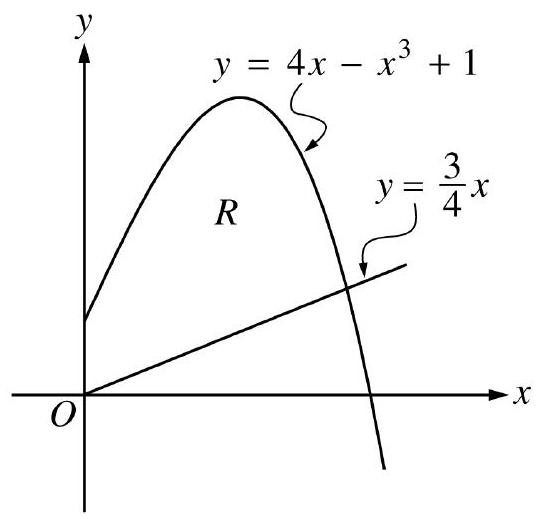
\includegraphics[width=0.6\linewidth]{figures/bc-2002-form-b_fig2.jpg}
\end{center}
Let $R$ be the region in the first quadrant bounded by the $y$-axis and the graphs of $y=4 x-x^{3}+1$ and $y=\frac{3}{4} x$.\\
\begin{parts}
\part Find the area of $R$.
\part Find the volume of the solid generated when $R$ is revolved about the $x$-axis.
\part Write an expression involving one or more integrals that gives the perimeter of $R$. Do not evaluate.
\end{parts}
\begin{solution}
\begin{parts}
\part Area $=\int_{0}^{A}\left(4 x-x^{3}+1-\frac{3}{4} x\right) d x$

\[=4.514 \text { or } 4.515\]
\part Volume

\[\begin{aligned}
& =\pi \int_{0}^{A}\left(\left(4 x-x^{3}+1\right)^{2}-\left(\frac{3}{4} x\right)^{2}\right) d x \\
& =18.291 \pi \text { or } 57.463
\end{aligned}\]
\part Perimeter $=1+\sqrt{(1.940)^{2}+(1.455)^{2}}$

\[+\int_{0}^{A} \sqrt{1+\left(4-3 x^{2}\right)^{2}} d x\]
\end{parts}
\par\medskip
\textbf{Rubric:}\par
\[\begin{aligned}
& 3\left\{\begin{array}{l}
1: \text { limits } \\
1: \text { integrand } \\
1: \text { answer }
\end{array}\right. \\
& 3\left\{\begin{array}{l}
1: \text { limits and constant } \\
1: \text { integrand } \\
1: \text { answer }
\end{array}\right. \\
& 3\left\{\begin{array}{l}
1: \text { uses } y^{\prime}=4-3 x^{2} \text { in integrand } \\
1: \text { arc length integral } \\
1: \text { answer }
\end{array}\right.
\end{aligned}\]
\end{solution}

\question
% Q4 | 2002 Calculus BC Form B | Part B | Calculator Prohibited
\begin{center}
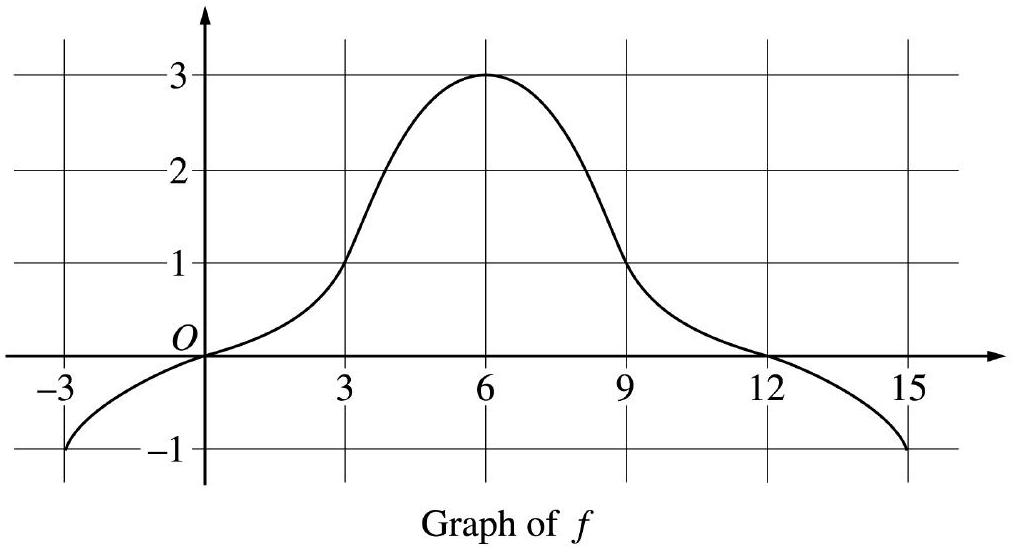
\includegraphics[width=0.6\linewidth]{figures/bc-2002-form-b_fig3.jpg}
\end{center}
The graph of a differentiable function $f$ on the closed interval $[-3,15]$ is shown in the figure above. The graph of $f$ has a horizontal tangent line at $x=6$. Let $g(x)=5+\int_{6}^{x} f(t) d t$ for $-3 \leq x \leq 15$.\\
\begin{parts}
\part Find $g(6), g^{\prime}(6)$, and $g^{\prime \prime}(6)$.
\part On what intervals is $g$ decreasing? Justify your answer.
\part On what intervals is the graph of $g$ concave down? Justify your answer.
\part Find a trapezoidal approximation of $\int_{-3}^{15} f(t) d t$ using six subintervals of length $\Delta t=3$.
\end{parts}
\begin{solution}
\begin{parts}
\part $g(6)=5+\int_{6}^{6} f(t) d t=5$

\begin{align*}& g^{\prime}(6)=f(6)=3 \\
& g^{\prime \prime}(6)=f^{\prime}(6)=0\end{align*}

\[3\left\{\begin{array}{l}
1: g(6) \\
1: g^{\prime}(6) \\
1: g^{\prime \prime}(6)
\end{array}\right.\]
\part $g$ is decreasing on $[-3,0]$ and $[12,15]$ since $g^{\prime}(x)=f(x)<0$ for $x<0$ and $x>12$.

\[3\left\{\begin{array}{l}
1:[-3,0] \\
1:[12,15] \\
1: \text { justification }
\end{array}\right.\]
\part The graph of $g$ is concave down on (6,15) since $g^{\prime}=f$ is decreasing on this interval.
\part $\frac{3}{2}(-1+2(0+1+3+1+0)-1)$
\end{parts}
\par\medskip
\textbf{Rubric:}\par
\begin{parts}
\part 1 : trapezoidal method $=12$
\end{parts}
\end{solution}

\question
% Q5 | 2002 Calculus BC Form B | Part B | Calculator Prohibited
Consider the differential equation $\frac{d y}{d x}=\frac{3-x}{y}$.\\
\begin{parts}
\part Let $y=f(x)$ be the particular solution to the given differential equation for $1<x<5$ such that the line $y=-2$ is tangent to the graph of $f$. Find the $x$-coordinate of the point of tangency, and determine whether $f$ has a local maximum, local minimum, or neither at this point. Justify your answer.
\part Let $y=g(x)$ be the particular solution to the given differential equation for $-2<x<8$, with the initial condition $g(6)=-4$. Find $y=g(x)$.
\end{parts}
\begin{solution}
\begin{parts}
\part $\frac{d y}{d x}=0$ when $x=3$

\[\left.\frac{d^{2} y}{d x^{2}}\right|_{(3,-2)}=\left.\frac{-y-y^{\prime}(3-x)}{y^{2}}\right|_{(3,-2)}=\frac{1}{2},\]

so $f$ has a local minimum at this point.\\
or\\
Because $f$ is continuous for $1<x<5$, there is an interval containing $x=3$ on which $y<0$. On this interval, $\frac{d y}{d x}$ is negative to the left of $x=3$ and $\frac{d y}{d x}$ is positive to the right of $x=3$. Therefore $f$ has a local minimum at $x=3$.
\part $y d y=(3-x) d x$

\begin{align*}& \frac{1}{2} y^{2}=3 x-\frac{1}{2} x^{2}+C \\
& 8=18-18+C ; C=8\end{align*}

\begin{align*}& y^{2}=6 x-x^{2}+16 \\
& y=-\sqrt{6 x-x^{2}+16}\end{align*}
\end{parts}
\par\medskip
\textbf{Rubric:}\par
\begin{parts}
\part $3\left\{\begin{array}{l}
1: x=3 \\
1: \text { local minimum } \\
1: \text { justification }
\end{array}\right.$
\part $6\left\{\begin{array}{l}
1: \text { separates variables } \\
1: \text { antiderivative of } d y \text { term } \\
1: \text { antiderivative of } d x \text { term } \\
1: \text { constant of integration } \\
1: \text { uses initial condition } g(6)=-4 \\
1: \text { solves for } y
\end{array}\right.$
\part Note: $\max 3 / 6[1-1-1-0-0-0]$ if no constant of integration
\part Note: $0 / 6$ if no separation of variables
\end{parts}
\end{solution}

\question
% Q6 | 2002 Calculus BC Form B | Part B | Calculator Prohibited
The Maclaurin series for $\ln \left(\frac{1}{1-x}\right)$ is $\sum_{n=1}^{\infty} \frac{x^{n}}{n}$ with interval of convergence $-1 \leq x<1$.\\
\begin{parts}
\part Find the Maclaurin series for $\ln \left(\frac{1}{1+3 x}\right)$ and determine the interval of convergence.
\part Find the value of $\sum_{n=1}^{\infty} \frac{(-1)^{n}}{n}$.
\part Give a value of $p$ such that $\sum_{n=1}^{\infty} \frac{(-1)^{n}}{n^{p}}$ converges, but $\sum_{n=1}^{\infty} \frac{1}{n^{2 p}}$ diverges. Give reasons why your value of $p$ is correct.
\part Give a value of $p$ such that $\sum_{n=1}^{\infty} \frac{1}{n^{p}}$ diverges, but $\sum_{n=1}^{\infty} \frac{1}{n^{2 p}}$ converges. Give reasons why your value of $p$ is correct.
\end{parts}
\begin{solution}
\begin{parts}
\part $\quad \ln \left(\frac{1}{1+3 x}\right)=\ln \left(\frac{1}{1-(-3 x)}\right)$

\[=\sum_{n=1}^{\infty} \frac{(-3 x)^{n}}{n} \text { or } \sum_{n=1}^{\infty}(-1)^{n} \frac{3^{n}}{n} x^{n}\]

We must have $-1 \leq-3 x<1$, so interval of convergence is $-\frac{1}{3}<x \leq \frac{1}{3}$.
\part $\quad \sum_{n=1}^{\infty} \frac{(-1)^{n}}{n}=\ln \left(\frac{1}{1-(-1)}\right)=\ln \left(\frac{1}{2}\right)$
\part Some $p$ such that $0<p \leq \frac{1}{2}$ because $\sum_{n=1}^{\infty} \frac{(-1)^{n}}{n^{p}}$ converges by AST, but the $p$-series $\sum_{n=1}^{\infty} \frac{1}{n^{2 p}}$ diverges for $2 p \leq 1$.
\part Some $p$ such that $\frac{1}{2}<p \leq 1$ because the $p$-series $\sum_{n=1}^{\infty} \frac{1}{n^{p}}$ diverges for $p \leq 1$ and the $p$-series $\sum_{n=1}^{\infty} \frac{1}{n^{2 p}}$ converges for $2 p>1$.
\end{parts}
\par\medskip
\textbf{Rubric:}\par
\begin{parts}
\part $2\left\{\begin{array}{l}
1: \text { series } \\
1: \text { interval of convergence }
\end{array}\right.$
\part 1 : answer
\part $3\left\{\begin{array}{l}
1: \text { correct } p \\
1: \text { reason why } \sum \frac{(-1)^{n}}{n^{p}} \text { converges } \\
1: \text { reason why } \sum \frac{1}{n^{2 p}} \text { diverges }
\end{array}\right.$
\part $3\left\{\begin{array}{l}
1: \text { correct } p \\
1: \text { reason why } \sum \frac{1}{n^{p}} \text { diverges } \\
1: \text { reason why } \sum \frac{1}{n^{2 p}} \text { converges }
\end{array}\right.$
\end{parts}
\end{solution}

\end{questions}

\section*{2003 AP Calculus BC}

\begin{questions}

\question
% Q1 | 2003 Calculus BC | Part A | Calculator Active
\begin{center}
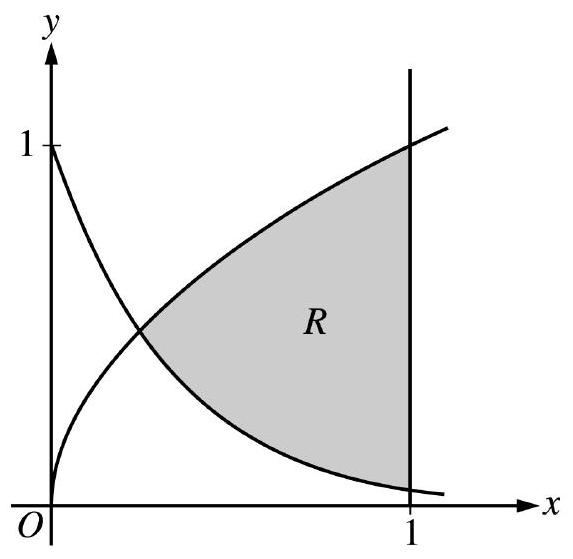
\includegraphics[width=0.6\linewidth]{figures/bc-2003_fig1.jpg}
\end{center}
Let $R$ be the shaded region bounded by the graphs of $y=\sqrt{x}$ and $y=e^{-3 x}$ and the vertical line $x=1$, as shown in the figure above.\\
\begin{parts}
\part Find the area of $R$.
\part Find the volume of the solid generated when $R$ is revolved about the horizontal line $y=1$.
\part The region $R$ is the base of a solid. For this solid, each cross section perpendicular to the $x$-axis is a rectangle whose height is 5 times the length of its base in region $R$. Find the volume of this solid.
\end{parts}
\begin{solution}
\begin{parts}
\part Area $=\int_{T}^{1}\left(\sqrt{x}-e^{-3 x}\right) d x$\\
$=0.442$ or 0.443
\part Volume $=\pi \int_{T}^{1}\left(\left(1-e^{-3 x}\right)^{2}-(1-\sqrt{x})^{2}\right) d x =0.453 \pi$ or 1.423 or 1.424
\part Length $=\sqrt{x}-e^{-3 x}$

Height $=5\left(\sqrt{x}-e^{-3 x}\right)$

Volume $=\int_{T}^{1} 5\left(\sqrt{x}-e^{-3 x}\right)^{2} d x=1.554$
\end{parts}
\par\medskip
\textbf{Rubric:}\par
\begin{parts}
\part 1: Correct limits in an integral in
\part $2:\left\{\begin{array}{l}1: \text { integrand } \\ 1: \text { answer }\end{array}\right.$
\part $3:\left\{\begin{aligned}
2: & \text { integrand } \\
& <-1>\text { reversal } \\
& <-1>\text { error with constant } \\
& <-1>\text { omits } 1 \text { in one radius } \\
& <-2>\text { other errors } \\
1: & \text { answer }
\end{aligned}\right.$
\part $3:\left\{\begin{aligned} 2: \text { integrand } & \\ & <-1> \\ & \\ & \sqrt{x}-e^{-3 x} \\ & \text { as a factor } \\ 1: \text { answer } & \end{aligned}\right.$
\end{parts}
\end{solution}

\question
% Q2 | 2003 Calculus BC | Part A | Calculator Active
\begin{center}
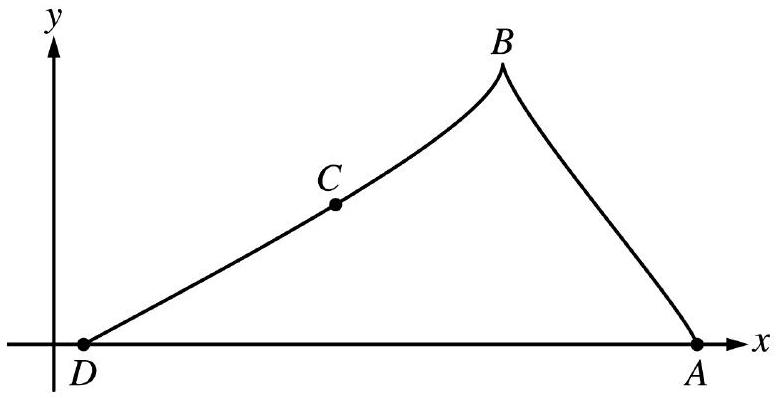
\includegraphics[width=0.6\linewidth]{figures/bc-2003_fig2.jpg}
\end{center}
A particle starts at point $A$ on the positive $x$-axis at time $t=0$ and travels along the curve from $A$ to $B$ to $C$ to $D$, as shown above. The coordinates of the particle's position $(x(t), y(t))$ are differentiable functions of $t$, where $x^{\prime}(t)=\frac{d x}{d t}=-9 \cos \left(\frac{\pi t}{6}\right) \sin \left(\frac{\pi \sqrt{t+1}}{2}\right)$ and $y^{\prime}(t)=\frac{d y}{d t}$ is not explicitly given. At time $t=9$, the particle reaches its final position at point $D$ on the positive $x$-axis.\\
\begin{parts}
\part At point $C$, is $\frac{d y}{d t}$ positive? At point $C$, is $\frac{d x}{d t}$ positive? Give a reason for each answer.
\part The slope of the curve is undefined at point $B$. At what time $t$ is the particle at point $B$ ?
\part The line tangent to the curve at the point $(x(8), y(8))$ has equation $y=\frac{5}{9} x-2$. Find the velocity vector and the speed of the particle at this point.
\part How far apart are points $A$ and $D$, the initial and final positions, respectively, of the particle?
\end{parts}
\begin{solution}
\begin{parts}
\part At point $C, \frac{d y}{d t}$ is not positive because $y(t)$ is decreasing along the arc $B D$ as $t$ increases.\\
At point $C, \frac{d x}{d t}$ is not positive because $x(t)$ is decreasing along the arc $B D$ as $t$ increases.
\part $\frac{d x}{d t}=0 ; \cos \left(\frac{\pi t}{6}\right)=0$ or $\sin \left(\frac{\pi \sqrt{t+1}}{2}\right)=0 \frac{\pi t}{6}=\frac{\pi}{2}$ or $\frac{\pi \sqrt{t+1}}{2}=\pi ; t=3$ for both.\\
Particle is at point $B$ at $t=3$.
\part $\quad x^{\prime}(8)=-9 \cos \left(\frac{4 \pi}{3}\right) \sin \left(\frac{3 \pi}{2}\right)=-\frac{9}{2}$

\begin{align*}& \frac{y^{\prime}(8)}{x^{\prime}(8)}=\frac{d y}{d x}=\frac{5}{9} \\
& y^{\prime}(8)=\frac{5}{9} x^{\prime}(8)=-\frac{5}{2}\end{align*}

$2:\left\{\begin{array}{l}1: \operatorname{sets} \frac{d x}{d t}=0 \\ 1: t=3\end{array}\right.$

The velocity vector is $\langle-4.5,-2.5\rangle$.\\
Speed $=\sqrt{4.5^{2}+2.5^{2}}=5.147$ or 5.148
\part $\quad x(9)-x(0)=\int_{0}^{9} x^{\prime}(t) d t$

\[=-39.255\]
\end{parts}
\par\medskip
\textbf{Rubric:}\par
\begin{parts}
\part $3:\left\{\begin{array}{l}1: x^{\prime}(8) \\ 1: y^{\prime}(8) \\ 1: \text { speed }\end{array}\right.$
\part $2:\left\{\begin{array}{l}1: \text { integral } \\ 1: \text { answer }\end{array}\right.$
\end{parts}
\end{solution}

\question
% Q3 | 2003 Calculus BC | Part A | Calculator Active
\begin{center}
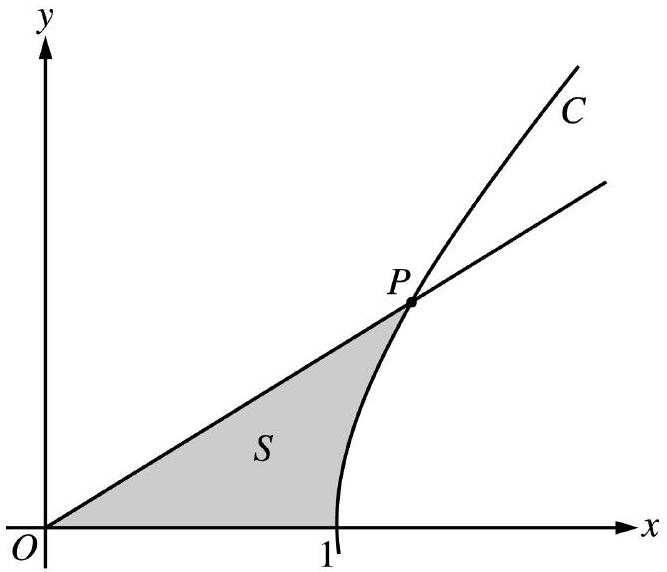
\includegraphics[width=0.6\linewidth]{figures/bc-2003_fig3.jpg}
\end{center}
The figure above shows the graphs of the line $x=\frac{5}{3} y$ and the curve $C$ given by $x=\sqrt{1+y^{2}}$. Let $S$ be the shaded region bounded by the two graphs and the $x$-axis. The line and the curve intersect at point $P$.\\
\begin{parts}
\part Find the coordinates of point $P$ and the value of $\frac{d x}{d y}$ for curve $C$ at point $P$.
\part Set up and evaluate an integral expression with respect to $y$ that gives the area of $S$.
\part Curve $C$ is a part of the curve $x^{2}-y^{2}=1$. Show that $x^{2}-y^{2}=1$ can be written as the polar equation $r^{2}=\frac{1}{\cos ^{2} \theta-\sin ^{2} \theta}$.
\part Use the polar equation given in part (c) to set up an integral expression with respect to the polar angle $\theta$ that represents the area of $S$.
\end{parts}
\begin{solution}
\begin{parts}
\part At $P, \frac{5}{3} y=\sqrt{1+y^{2}}$, so $y=\frac{3}{4}$.

Since $x=\frac{5}{3} y, x=\frac{5}{4}$.

\[\frac{d x}{d y}=\frac{y}{\sqrt{1+y^{2}}}=\frac{y}{x} . \text { At } P, \frac{d x}{d y}=\frac{3 / 4}{5 / 4}=\frac{3}{5} .\]
\part Area $=\int_{0}^{3 / 4}\left(\sqrt{1+y^{2}}-\frac{5}{3} y\right) d y$

\[=0.346 \text { or } 0.347\]
\part $x=r \cos \theta ; y=r \sin \theta$

\begin{align*}& x^{2}-y^{2}=1 \Rightarrow r^{2} \cos ^{2} \theta-r^{2} \sin ^{2} \theta=1 \\
& r^{2}=\frac{1}{\cos ^{2} \theta-\sin ^{2} \theta}\end{align*}
\part Let $\beta$ be the angle that segment $O P$ makes with the $x$-axis. Then $\tan \beta=\frac{y}{x}=\frac{3 / 4}{5 / 4}=\frac{3}{5}$.

\begin{align*}\text { Area } & =\int_{0}^{\tan ^{-1}(3 / 5)} \frac{1}{2} r^{2} d \theta \\
& =\frac{1}{2} \int_{0}^{\tan ^{-1}(3 / 5)} \frac{1}{\cos ^{2} \theta-\sin ^{2} \theta} d \theta\end{align*}
\end{parts}
\par\medskip
\textbf{Rubric:}\par
\begin{parts}
\part $2:\left\{\begin{array}{l}
1: \text { coordinates of } P \\
1: \frac{d x}{d y} \text { at } P
\end{array}\right.$
\part $3:\left\{\begin{array}{l}1: \text { limits } \\ 1: \text { integrand } \\ 1: \text { answer }\end{array}\right.$
\part $2:\left\{\begin{array}{c}1: \text { substitutes } x=r \cos \theta \text { and } \\ y=r \sin \theta \text { into } x^{2}-y^{2}=1 \\ 1: \text { isolates } r^{2}\end{array}\right.$
\part $2:\left\{\begin{array}{l}
1: \text { limits } \\
1: \text { integrand and constant }
\end{array}\right.$
\end{parts}
\end{solution}

\question
% Q4 | 2003 Calculus BC | Part B | Calculator Prohibited
\begin{center}
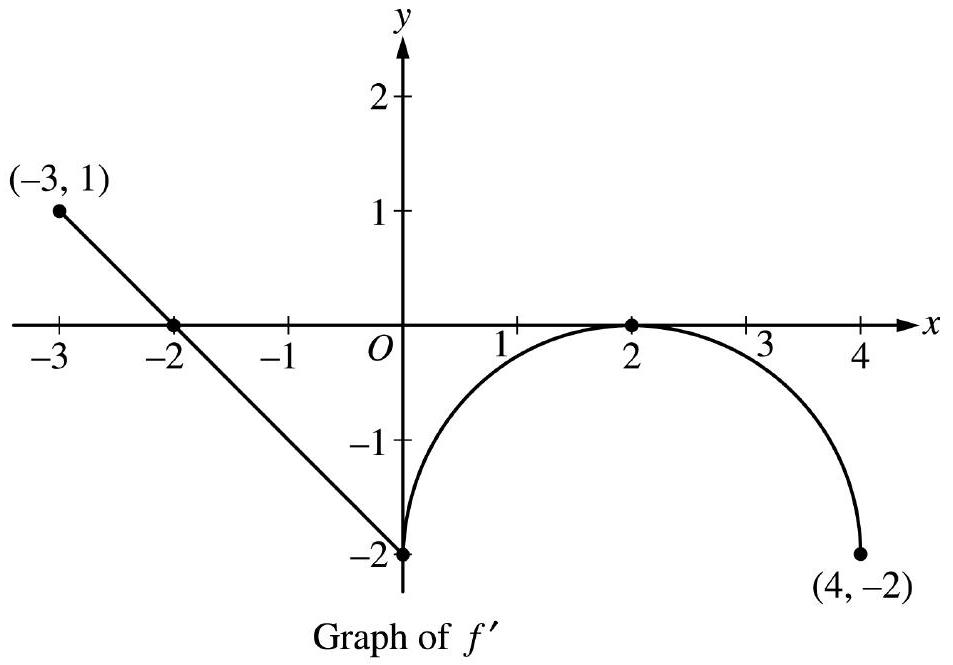
\includegraphics[width=0.6\linewidth]{figures/bc-2003_fig4.jpg}
\end{center}
Let $f$ be a function defined on the closed interval $-3 \leq x \leq 4$ with $f(0)=3$. The graph of $f^{\prime}$, the derivative of $f$, consists of one line segment and a semicircle, as shown above.\\
\begin{parts}
\part On what intervals, if any, is $f$ increasing? Justify your answer.
\part Find the $x$-coordinate of each point of inflection of the graph of $f$ on the open interval $-3<x<4$. Justify your answer.
\part Find an equation for the line tangent to the graph of $f$ at the point ( 0,3 ).
\part Find $f(-3)$ and $f(4)$. Show the work that leads to your answers.
\end{parts}
\begin{solution}
\begin{parts}
\part The function $f$ is increasing on $[-3,-2]$ since $f^{\prime}>0$ for $-3 \leq x<-2$.
\part $\quad x=0$ and $x=2$\\
$f^{\prime}$ changes from decreasing to increasing at $x=0$ and from increasing to decreasing at $x=2$
\part $f^{\prime}(0)=-2$

Tangent line is $y=-2 x+3$.
\part $f(0)-f(-3)=\int_{-3}^{0} f^{\prime}(t) d t$

\[=\frac{1}{2}(1)(1)-\frac{1}{2}(2)(2)=-\frac{3}{2}\]

$f(-3)=f(0)+\frac{3}{2}=\frac{9}{2}$

\[\begin{aligned}
f(4)-f(0) & =\int_{0}^{4} f^{\prime}(t) d t \\
& =-\left(8-\frac{1}{2}(2)^{2} \pi\right)=-8+2 \pi
\end{aligned}\]

$f(4)=f(0)-8+2 \pi=-5+2 \pi$
\end{parts}
\par\medskip
\textbf{Rubric:}\par
\begin{parts}
\part $2:\left\{\begin{array}{l}
1: \text { interval } \\
1: \text { reason }
\end{array}\right.$
\part $2:\left\{\begin{array}{l}1: x=0 \text { and } x=2 \text { only } \\ 1: \text { justification }\end{array}\right.$
\part 1 : equation
\part $1: \pm\left(\frac{1}{2}-2\right)$
\part 1 : answer for $f(-3)$ using FTC
\part $1: \pm\left(8-\frac{1}{2}(2)^{2} \pi\right)$
\part 1 : answer for $f(4)$ using FTC
\end{parts}
\end{solution}

\question
% Q5 | 2003 Calculus BC | Part B | Calculator Prohibited
\begin{center}
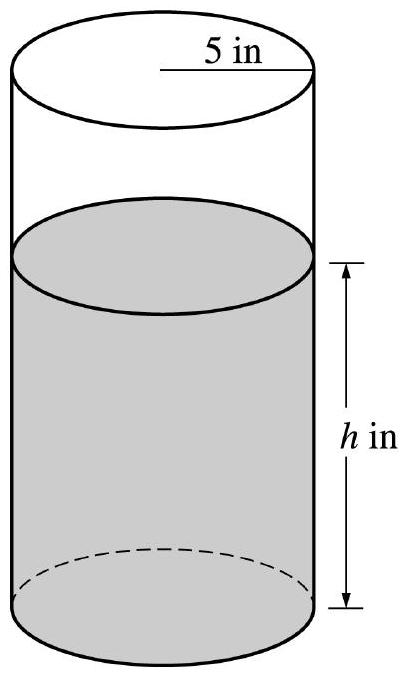
\includegraphics[width=0.6\linewidth]{figures/bc-2003_fig5.jpg}
\end{center}
A coffeepot has the shape of a cylinder with radius 5 inches, as shown in the figure above. Let $h$ be the depth of the coffee in the pot, measured in inches, where $h$ is a function of time $t$, measured in seconds. The volume $V$ of coffee in the pot is changing at the rate of $-5 \pi \sqrt{h}$ cubic inches per second. (The volume $V$ of a cylinder with radius $r$ and height $h$ is $V=\pi r^{2} h$.)\\
\begin{parts}
\part Show that $\frac{d h}{d t}=-\frac{\sqrt{h}}{5}$.
\part Given that $h=17$ at time $t=0$, solve the differential equation $\frac{d h}{d t}=-\frac{\sqrt{h}}{5}$ for $h$ as a function of $t$.
\part At what time $t$ is the coffeepot empty?
\end{parts}
\begin{solution}
\begin{parts}
\part $V=25 \pi h$

\begin{align*}& \frac{d V}{d t}=25 \pi \frac{d h}{d t}=-5 \pi \sqrt{h} \\
& \frac{d h}{d t}=\frac{-5 \pi \sqrt{h}}{25 \pi}=-\frac{\sqrt{h}}{5}\end{align*}
\part $\frac{d h}{d t}=-\frac{\sqrt{h}}{5}$

\[\begin{aligned}
& \frac{1}{\sqrt{h}} d h=-\frac{1}{5} d t \\
& 2 \sqrt{h}=-\frac{1}{5} t+C \\
& 2 \sqrt{17}=0+C \\
& h=\left(-\frac{1}{10} t+\sqrt{17}\right)^{2}
\end{aligned}\]
\part $\left(-\frac{1}{10} t+\sqrt{17}\right)^{2}=0$

\[t=10 \sqrt{17}\]
\end{parts}
\par\medskip
\textbf{Rubric:}\par
\begin{parts}
\part $3:\left\{\begin{array}{l}1: \frac{d V}{d t}=-5 \pi \sqrt{h} \\ 1: \text { computes } \frac{d V}{d t} \\ 1: \text { shows result }\end{array}\right.$
\part $5:\left\{\begin{array}{l}1: \text { separates variables } \\ 1: \text { antiderivatives } \\ 1: \text { constant of integration } \\ 1: \text { uses initial condition } h=17 \\ \quad \text { when } t=0 \\ 1: \text { solves for } h\end{array}\right.$
\part Note: $\max 2 / 5[1-1-0-0-0]$ if no constant of integration
\part Note: $0 / 5$ if no separation of variables
\part 1 : answer
\end{parts}
\end{solution}

\question
% Q6 | 2003 Calculus BC | Part B | Calculator Prohibited
The function $f$ is defined by the power series

\[f(x)=\sum_{n=0}^{\infty} \frac{(-1)^{n} x^{2 n}}{(2 n+1)!}=1-\frac{x^{2}}{3!}+\frac{x^{4}}{5!}-\frac{x^{6}}{7!}+\cdots+\frac{(-1)^{n} x^{2 n}}{(2 n+1)!}+\cdots\]

for all real numbers $x$.\\
\begin{parts}
\part Find $f^{\prime}(0)$ and $f^{\prime \prime}(0)$. Determine whether $f$ has a local maximum, a local minimum, or neither at $x=0$. Give a reason for your answer.
\part Show that $1-\frac{1}{3!}$ approximates $f(1)$ with error less than $\frac{1}{100}$.
\part Show that $y=f(x)$ is a solution to the differential equation $x y^{\prime}+y=\cos x$.
\end{parts}
\begin{solution}
\begin{center}
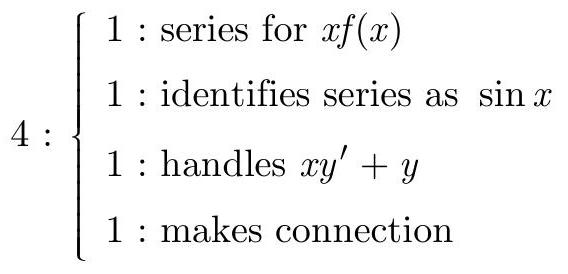
\includegraphics[width=0.6\linewidth]{figures/sg-bc-2003_fig6.jpg}
\end{center}
\begin{parts}
\part $f^{\prime}(0)=$ coefficient of $x$ term $=0 f^{\prime \prime}(0)=2\left(\right.$ coefficient of $x^{2}$ term $)=2\left(-\frac{1}{3!}\right)=-\frac{1}{3} f$ has a local maximum at $x=0$ because $f^{\prime}(0)=0$ and $f^{\prime \prime}(0)<0$.
\part $f(1)=1-\frac{1}{3!}+\frac{1}{5!}-\frac{1}{7!}+\cdots+\frac{(-1)^{n}}{(2 n+1)!}+\cdots$ 1 : error bound $<\frac{1}{100}$

This is an alternating series whose terms decrease in absolute value with limit 0 . Thus, the error is less than the first omitted term, so $\left|f(1)-\left(1-\frac{1}{3!}\right)\right| \leq \frac{1}{5!}=\frac{1}{120}<\frac{1}{100}$.
\part $\quad y^{\prime}=-\frac{2 x}{3!}+\frac{4 x^{3}}{5!}-\frac{6 x^{5}}{7!}+\cdots+\frac{(-1)^{n} 2 n x^{2 n-1}}{(2 n+1)!}+\cdots$

\[\begin{aligned}
x y^{\prime}= & -\frac{2 x^{2}}{3!}+\frac{4 x^{4}}{5!}-\frac{6 x^{6}}{7!}+\cdots+\frac{(-1)^{n} 2 n x^{2 n}}{(2 n+1)!}+\cdots \\
x y^{\prime}+y= & 1-\left(\frac{2}{3!}+\frac{1}{3!}\right) x^{2}+\left(\frac{4}{5!}+\frac{1}{5!}\right) x^{4}-\left(\frac{6}{7!}+\frac{1}{7!}\right) x^{6}+\cdots \\
& \quad+(-1)^{n}\left(\frac{2 n}{(2 n+1)!}+\frac{1}{(2 n+1)!}\right) x^{2 n}+\cdots \\
= & 1-\frac{1}{2!} x^{2}+\frac{1}{4!} x^{4}-\frac{1}{6!} x^{6}+\cdots+\frac{(-1)^{n}}{(2 n)!} x^{2 n}+\cdots \\
= & \cos x
\end{aligned}\]

OR

\begin{align*}& x y=x f(x)=x-\frac{x^{3}}{3!}+\cdots+(-1)^{n} \frac{1}{(2 n+1)!} x^{2 n+1}+\cdots \\
& \quad=\sin x \\
& x y^{\prime}+y=(x y)^{\prime}=(\sin x)^{\prime}=\cos x\end{align*}

OR
\end{parts}
\end{solution}

\end{questions}

\section*{2003 AP Calculus BC Form B}

\begin{questions}

\question
% Q1 | 2003 Calculus BC Form B | Part A | Calculator Active
\begin{center}
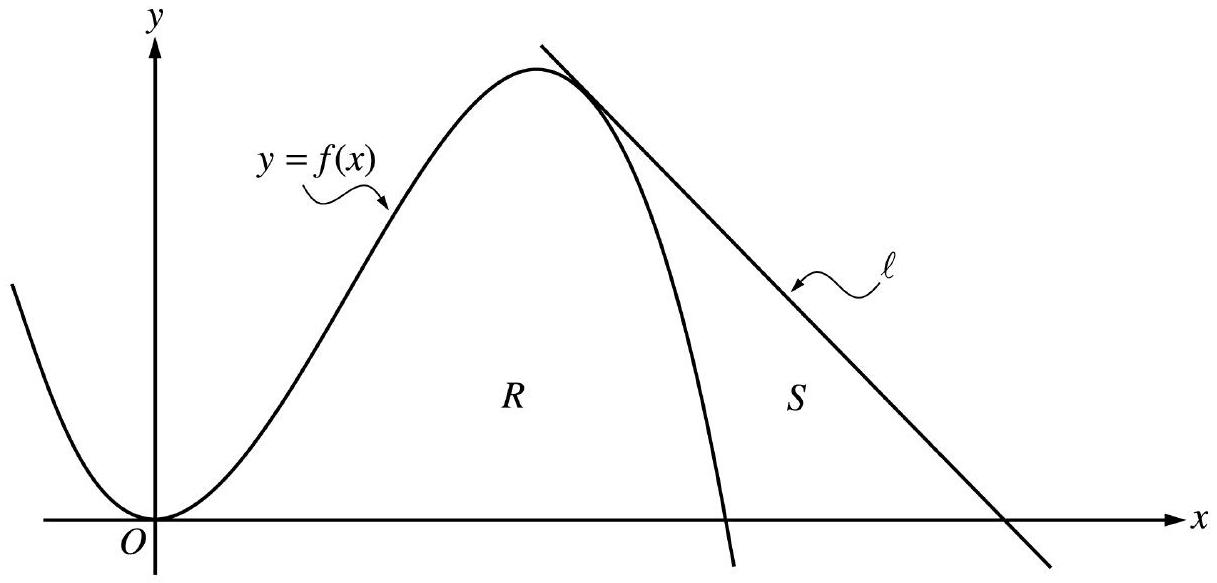
\includegraphics[width=0.6\linewidth]{figures/bc-2003-form-b_fig1.jpg}
\end{center}
Let $f$ be the function given by $f(x)=4 x^{2}-x^{3}$, and let $\ell$ be the line $y=18-3 x$, where $\ell$ is tangent to the graph of $f$. Let $R$ be the region bounded by the graph of $f$ and the $x$-axis, and let $S$ be the region bounded by the graph of $f$, the line $\ell$, and the $x$-axis, as shown above.\\
\begin{parts}
\part Show that $\ell$ is tangent to the graph of $y=f(x)$ at the point $x=3$.
\part Find the area of $S$.
\part Find the volume of the solid generated when $R$ is revolved about the $x$-axis.
\end{parts}
\begin{solution}
\begin{parts}
\part $f^{\prime}(x)=8 x-3 x^{2} ; f^{\prime}(3)=24-27=-3$\\
$f(3)=36-27=9$\\
Tangent line at $x=3$ is\\
$y=-3(x-3)+9=-3 x+18$,\\
which is the equation of line $\ell$.
\part $\quad f(x)=0$ at $x=4$

The line intersects the $x$-axis at $x=6$.

\[\begin{aligned}
\text { Area } & =\frac{1}{2}(3)(9)-\int_{3}^{4}\left(4 x^{2}-x^{3}\right) d x \\
& =7.916 \text { or } 7.917
\end{aligned}\]

OR

\[\begin{aligned}
\text { Area }= & \int_{3}^{4}\left((18-3 x)-\left(4 x^{2}-x^{3}\right)\right) d x \\
& +\frac{1}{2}(2)(18-12) \\
= & 7.916 \text { or } 7.917
\end{aligned}\]
\part Volume $=\pi \int_{0}^{4}\left(4 x^{2}-x^{3}\right)^{2} d x$

\[=156.038 \pi \text { or } 490.208\]
\end{parts}
\par\medskip
\textbf{Rubric:}\par
\[\begin{aligned}
& 2:\left\{\begin{array}{c}
1: \text { finds } f^{\prime}(3) \text { and } f(3) \\
1:\left\{\begin{array}{c}
\text { finds equation of tangent line } \\
\text { or } \\
\text { shows }(3,9) \text { is on both the } \\
\text { graph of } f \text { and line } \ell
\end{array}\right. \\
4:\left\{\begin{array}{c}
2: \text { integral for non-triangular region } \\
1: \text { limits } \\
1: \text { integrand } \\
1: \text { area of triangular region } \\
1: \text { answer }
\end{array}\right. \\
3:\left\{\begin{array}{l}
1: \text { limits and constant } \\
1: \text { integrand } \\
1: \text { answer }
\end{array}\right.
\end{array}\right.
\end{aligned}\]
\end{solution}

\question
% Q2 | 2003 Calculus BC Form B | Part A | Calculator Active
\begin{center}
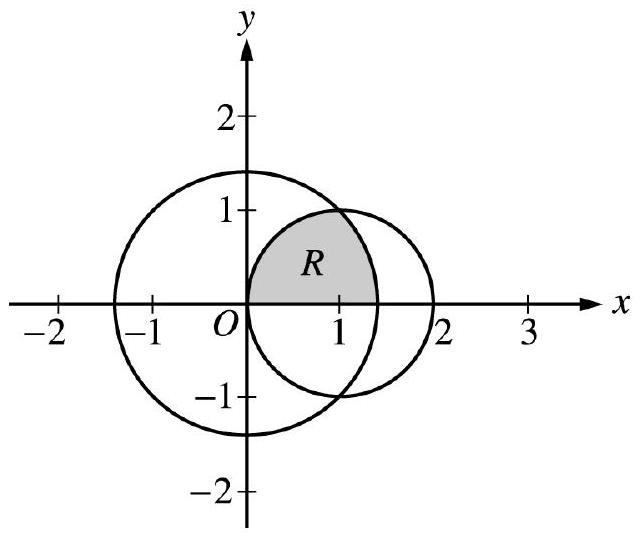
\includegraphics[width=0.6\linewidth]{figures/bc-2003-form-b_fig2.jpg}
\end{center}
The figure above shows the graphs of the circles $x^{2}+y^{2}=2$ and $(x-1)^{2}+y^{2}=1$. The graphs intersect at the points $(1,1)$ and $(1,-1)$. Let $R$ be the shaded region in the first quadrant bounded by the two circles and the $x$-axis.\\
\begin{parts}
\part Set up an expression involving one or more integrals with respect to $x$ that represents the area of $R$.
\part Set up an expression involving one or more integrals with respect to $y$ that represents the area of $R$.
\part The polar equations of the circles are $r=\sqrt{2}$ and $r=2 \cos \theta$, respectively. Set up an expression involving one or more integrals with respect to the polar angle $\theta$ that represents the area of $R$.
\end{parts}
\begin{solution}
\begin{parts}
\part Area $=\int_{0}^{1} \sqrt{1-(x-1)^{2}} d x+\int_{1}^{\sqrt{2}} \sqrt{2-x^{2}} d x$

Area $=\frac{1}{4}\left(\pi \cdot 1^{2}\right)+\int_{1}^{\sqrt{2}} \sqrt{2-x^{2}} d x$
\part Area $=\int_{0}^{1}\left(\sqrt{2-y^{2}}-\left(1-\sqrt{1-y^{2}}\right)\right) d y$

\[3:\left\{\begin{aligned}
1: & \text { integrand for larger circle } \\
1: & \text { integrand or geometric area } \\
& \text { for smaller circle } \\
1: & \text { limits on integral(s) }
\end{aligned}\right.\]

Note: $\langle-1\rangle$ if no addition of terms

\[3:\left\{\begin{aligned}
1: & \text { limits } \\
2: & \text { integrand } \\
& <-1>\text { reversal } \\
& <-1>\text { algebra error } \\
& \text { in solving for } x \\
< & -1>\text { add rather } \\
& \text { than subtract } \\
< & -2>\text { other errors }
\end{aligned}\right.\]

\[3:\left\{\begin{aligned}
1: & \text { integrand or geometric area } \\
& \text { for larger circle } \\
1: & \text { integrand for smaller circle } \\
1: & \text { limits on integral(s) }
\end{aligned}\right.\]

Note: $<-1>$ if no addition of terms
\part Area $=\int_{0}^{\pi / 4} \frac{1}{2}(\sqrt{2})^{2} d \theta+\int_{\pi / 4}^{\pi / 2} \frac{1}{2}(2 \cos \theta)^{2} d \theta$

\[\text { Area }=\frac{1}{8} \pi(\sqrt{2})^{2}+\int_{\pi / 4}^{\pi / 2} \frac{1}{2}(2 \cos \theta)^{2} d \theta\]
\end{parts}
\end{solution}

\question
% Q3 | 2003 Calculus BC Form B | Part A | Calculator Active
\begin{center}
\begin{tabular}{|c|c|c|c|c|c|c|c|}
\hline
\begin{tabular}{c}
Distance \\
$x$ \\
$(\mathrm{~mm})$ \\
\end{tabular} & 0 & 60 & 120 & 180 & 240 & 300 & 360 \\
\hline
\begin{tabular}{c}
Diameter \\
$B(x)$ \\
$(\mathrm{mm})$ \\
\end{tabular} & 24 & 30 & 28 & 30 & 26 & 24 & 26 \\
\hline
\end{tabular}
\end{center}
A blood vessel is 360 millimeters ( mm ) long with circular cross sections of varying diameter. The table above gives the measurements of the diameter of the blood vessel at selected points along the length of the blood vessel, where $x$ represents the distance from one end of the blood vessel and $B(x)$ is a twice-differentiable function that represents the diameter at that point.\\
\begin{parts}
\part Write an integral expression in terms of $B(x)$ that represents the average radius, in mm , of the blood vessel between $x=0$ and $x=360$.
\part Approximate the value of your answer from part (a) using the data from the table and a midpoint Riemann sum with three subintervals of equal length. Show the computations that lead to your answer.
\part Using correct units, explain the meaning of $\pi \int_{125}^{275}\left(\frac{B(x)}{2}\right)^{2} d x$ in terms of the blood vessel.
\part Explain why there must be at least one value $x$, for $0<x<360$, such that $B^{\prime \prime}(x)=0$.
\end{parts}
\begin{solution}
\begin{parts}
\part $\frac{1}{360} \int_{0}^{360} \frac{B(x)}{2} d x$
\part $\frac{1}{360}\left[120\left(\frac{B(60)}{2}+\frac{B(180)}{2}+\frac{B(300)}{2}\right)\right]= \frac{1}{360}[60(30+30+24)]=14$
\part $\frac{B(x)}{2}$ is the radius, so $\pi\left(\frac{B(x)}{2}\right)^{2}$ is the area of the cross section at $x$. The expression is the volume in $\mathrm{mm}^{3}$ of the blood vessel between 125 mm and 275 mm from the end of the vessel.
\part By the MVT, $B^{\prime}\left(c_{1}\right)=0$ for some $c_{1}$ in $(60,180)$ and $B^{\prime}\left(c_{2}\right)=0$ for some $c_{2}$ in $(240,360)$. The MVT applied to $B^{\prime}(x)$ shows that $B^{\prime \prime}(x)=0$ for some $x$ in the interval $\left(c_{1}, c_{2}\right)$.
\end{parts}
\par\medskip
\textbf{Rubric:}\par
\begin{parts}
\part 1: B(60)+B(180)+B(300)
\part Note: $\max 1 / 3$ if only explains why
\end{parts}
\end{solution}

\question
% Q4 | 2003 Calculus BC Form B | Part B | Calculator Prohibited
A particle moves in the $x y$-plane so that the position of the particle at any time $t$ is given by

\[x(t)=2 e^{3 t}+e^{-7 t} \text { and } y(t)=3 e^{3 t}-e^{-2 t} .\]
\begin{parts}
\part Find the velocity vector for the particle in terms of $t$, and find the speed of the particle at time $t=0$.
\part Find $\frac{d y}{d x}$ in terms of $t$, and find $\lim _{t \rightarrow \infty} \frac{d y}{d x}$.
\part Find each value $t$ at which the line tangent to the path of the particle is horizontal, or explain why none exists.
\part Find each value $t$ at which the line tangent to the path of the particle is vertical, or explain why none exists.
\end{parts}
\begin{solution}
\begin{parts}
\part $\quad x^{\prime}(t)=6 e^{3 t}-7 e^{-7 t}$\\
$y^{\prime}(t)=9 e^{3 t}+2 e^{-2 t}$\\
Velocity vector is $<6 e^{3 t}-7 e^{-7 t}, 9 e^{3 t}+2 e^{-2 t}>$

\begin{align*}\text { Speed } & =\sqrt{x^{\prime}(0)^{2}+y^{\prime}(0)^{2}}=\sqrt{(-1)^{2}+11^{2}} \\
& =\sqrt{122}\end{align*}
\part $\frac{d y}{d x}=\frac{\frac{d y}{d t}}{\frac{d x}{d t}}=\frac{9 e^{3 t}+2 e^{-2 t}}{6 e^{3 t}-7 e^{-7 t}}$

\[\lim _{t \rightarrow \infty} \frac{d y}{d x}=\lim _{t \rightarrow \infty} \frac{9 e^{3 t}+2 e^{-2 t}}{6 e^{3 t}-7 e^{-7 t}}=\frac{9}{6}=\frac{3}{2}\]
\part Need $y^{\prime}(t)=0$, but $9 e^{3 t}+2 e^{-2 t}>0$ for all $t$, so none exists.
\part Need $x^{\prime}(t)=0$ and $y^{\prime}(t) \neq 0$.
\end{parts}
\par\medskip
\textbf{Rubric:}\par
\begin{parts}
\part $1: x^{\prime}(t)$
\part $1: y^{\prime}(t)$
\end{parts}
\end{solution}

\question
% Q5 | 2003 Calculus BC Form B | Part B | Calculator Prohibited
\begin{center}
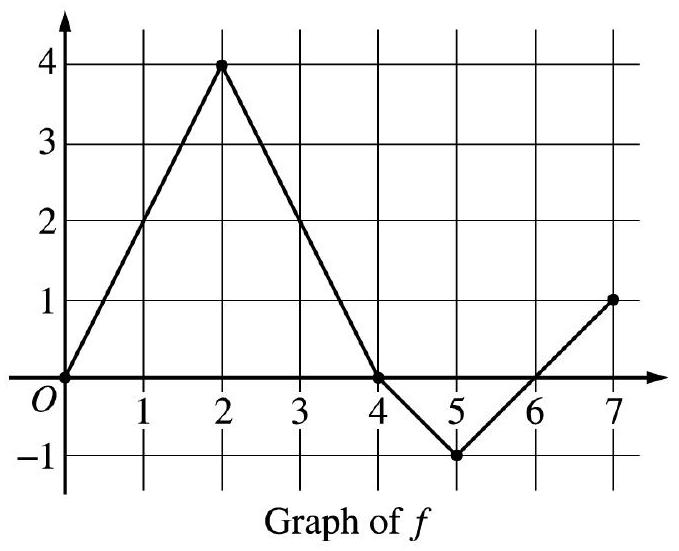
\includegraphics[width=0.6\linewidth]{figures/bc-2003-form-b_fig3.jpg}
\end{center}
Let $f$ be a function defined on the closed interval $[0,7]$. The graph of $f$, consisting of four line segments, is shown above. Let $g$ be the function given by $g(x)=\int_{2}^{x} f(t) d t$.\\
\begin{parts}
\part Find $g(3), g^{\prime}(3)$, and $g^{\prime \prime}(3)$.
\part Find the average rate of change of $g$ on the interval $0 \leq x \leq 3$.
\part For how many values $c$, where $0<c<3$, is $g^{\prime}(c)$ equal to the average rate found in part (b) ? Explain your reasoning.
\part Find the $x$-coordinate of each point of inflection of the graph of $g$ on the interval $0<x<7$. Justify your answer.
\end{parts}
\begin{solution}
\begin{parts}
\part $g(3)=\int_{2}^{3} f(t) d t=\frac{1}{2}(4+2)=3$

\begin{align*}& g^{\prime}(3)=f(3)=2 \\
& g^{\prime \prime}(3)=f^{\prime}(3)=\frac{0-4}{4-2}=-2\end{align*}
\part $\frac{g(3)-g(0)}{3}=\frac{1}{3} \int_{0}^{3} f(t) d t$

\[=\frac{1}{3}\left(\frac{1}{2}(2)(4)+\frac{1}{2}(4+2)\right)=\frac{7}{3}\]
\part There are two values of $c$.

We need $\frac{7}{3}=g^{\prime}(c)=f(c)$\\
The graph of $f$ intersects the line $y=\frac{7}{3}$ at two places between 0 and 3 .
\part $\quad x=2$ and $x=5$\\
because $g^{\prime}=f$ changes from increasing to decreasing at $x=2$, and from decreasing to increasing at $x=5$.
\end{parts}
\par\medskip
\textbf{Rubric:}\par
\begin{parts}
\part $3:\left\{\begin{array}{l}1: g(3) \\ 1: g^{\prime}(3) \\ 1: g^{\prime \prime}(3)\end{array}\right.$
\part $2:\left\{\begin{array}{l}1: g(3)-g(0)=\int_{0}^{3} f(t) d t \\ 1: \text { answer }\end{array}\right.$
\part $2:\left\{\begin{array}{l}1: \text { answer of } 2 \\ 1: \text { reason }\end{array}\right.$
\part Note: $1 / 2$ if answer is 1 by MVT
\part $2:\left\{\begin{aligned} 1: & x=2 \text { and } x=5 \text { only } \\ 1: & \text { justification } \\ & (\text { ignore discussion at } x=4)\end{aligned}\right.$
\end{parts}
\end{solution}

\question
% Q6 | 2003 Calculus BC Form B | Part B | Calculator Prohibited
The function $f$ has a Taylor series about $x=2$ that converges to $f(x)$ for all $x$ in the interval of convergence.

The $n$th derivative of $f$ at $x=2$ is given by $f^{(n)}(2)=\frac{(n+1)!}{3^{n}}$ for $n \geq 1$, and $f(2)=1$.\\
\begin{parts}
\part Write the first four terms and the general term of the Taylor series for $f$ about $x=2$.
\part Find the radius of convergence for the Taylor series for $f$ about $x=2$. Show the work that leads to your answer.
\part Let $g$ be a function satisfying $g(2)=3$ and $g^{\prime}(x)=f(x)$ for all $x$. Write the first four terms and the general term of the Taylor series for $g$ about $x=2$.
\part Does the Taylor series for $g$ as defined in part (c) converge at $x=-2$ ? Give a reason for your answer.
\end{parts}
\begin{solution}
\begin{parts}
\part $f(2)=1 ; f^{\prime}(2)=\frac{2!}{3} ; f^{\prime \prime}(2)=\frac{3!}{3^{2}} ; f^{\prime \prime \prime}(2)=\frac{4!}{3^{3}}$

\[\begin{gathered}
f(x)=1+\frac{2}{3}(x-2)+\frac{3!}{2!3^{2}}(x-2)^{2}+\frac{4!}{3!3^{3}}(x-2)^{3}+ \\
+\cdots+\frac{(n+1)!}{n!3^{n}}(x-2)^{n}+\cdots \\
=1+\frac{2}{3}(x-2)+\frac{3}{3^{2}}(x-2)^{2}+\frac{4}{3^{3}}(x-2)^{3}+ \\
+\cdots+\frac{n+1}{3^{n}}(x-2)^{n}+\cdots
\end{gathered}\]
\part $\lim _{n \rightarrow \infty}\left|\frac{\frac{n+2}{3^{n+1}}(x-2)^{n+1}}{\frac{n+1}{3^{n}}(x-2)^{n}}\right|=\lim _{n \rightarrow \infty} \frac{n+2}{n+1} \cdot \frac{1}{3}|x-2|$\\
$=\frac{1}{3}|x-2|<1$ when $|x-2|<3$\\
The radius of convergence is 3 .
\part $g(2)=3 ; g^{\prime}(2)=f(2) ; g^{\prime \prime}(2)=f^{\prime}(2) ; g^{\prime \prime \prime}(2)=f^{\prime \prime}(2) g(x)=3+(x-2)+\frac{1}{3}(x-2)^{2}+\frac{1}{3^{2}}(x-2)^{3}+ +\cdots+\frac{1}{3^{n}}(x-2)^{n+1}+\cdots$
\part No, the Taylor series does not converge at $x=-2$ because the geometric series only converges on the interval $|x-2|<3$.\\
( 1 : coefficients $\frac{f^{(n)}(2)}{n!}$ in first four terms $3: \quad 1:$ powers of $(x-2)$ in first four terms 1 : general term
\end{parts}
\par\medskip
\textbf{Rubric:}\par
\begin{parts}
\part $3:\left\{\begin{array}{l}1: \text { sets up ratio } \\ 1: \text { limit } \\ 1: \text { applies ratio test to } \\ \text { conclude radius of } \\ \text { convergence is } 3\end{array}\right.$
\part $2:\left\{\begin{array}{l}1: \text { first four terms } \\ 1: \text { general term }\end{array}\right.$
\part 1 : answer with reason
\end{parts}
\end{solution}

\end{questions}

\section*{2004 AP Calculus BC}

\begin{questions}

\question
% Q1 | 2004 Calculus BC | Part A | Calculator Active
Traffic flow is defined as the rate at which cars pass through an intersection, measured in cars per minute. The traffic flow at a particular intersection is modeled by the function $F$ defined by
\[F(t)=82+4 \sin \left(\frac{t}{2}\right) \text { for } 0 \leq t \leq 30\]

where $F(t)$ is measured in cars per minute and $t$ is measured in minutes.\\
\begin{parts}
\part To the nearest whole number, how many cars pass through the intersection over the 30 -minute period?
\part Is the traffic flow increasing or decreasing at $t=7$ ? Give a reason for your answer.
\part What is the average value of the traffic flow over the time interval $10 \leq t \leq 15$ ? Indicate units of measure.
\part What is the average rate of change of the traffic flow over the time interval $10 \leq t \leq 15$ ? Indicate units of measure.
\end{parts}
\begin{solution}
\begin{parts}
\part $\quad \int_{0}^{30} F(t) d t=2474$ cars
\part $F^{\prime}(7)=-1.872$ or -1.873

Since $F^{\prime}(7)<0$, the traffic flow is decreasing at $t=7$.
\part $\frac{1}{5} \int_{10}^{15} F(t) d t=81.899 \mathrm{cars} / \mathrm{min}$
\part $\frac{F(15)-F(10)}{15-10}=1.517$ or $1.518 \mathrm{cars} / \mathrm{min}^{2}$

Units of cars / min in (c) and cars / $\min ^{2}$ in (d)
\end{parts}
\par\medskip
\textbf{Rubric:}\par
\begin{parts}
\part $3:\left\{\begin{array}{l}
1: \text { limits } \\
1: \text { integrand } \\
1: \text { answer }
\end{array}\right.$
\part 1 : answer with reason
\part $3:\left\{\begin{array}{l}1: \text { limits } \\ 1: \text { integrand } \\ 1: \text { answer }\end{array}\right.$
\part 1 : answer
\part 1 : units in (c) and (d)
\end{parts}
\end{solution}

\question
% Q2 | 2004 Calculus BC | Part A | Calculator Active
\begin{center}
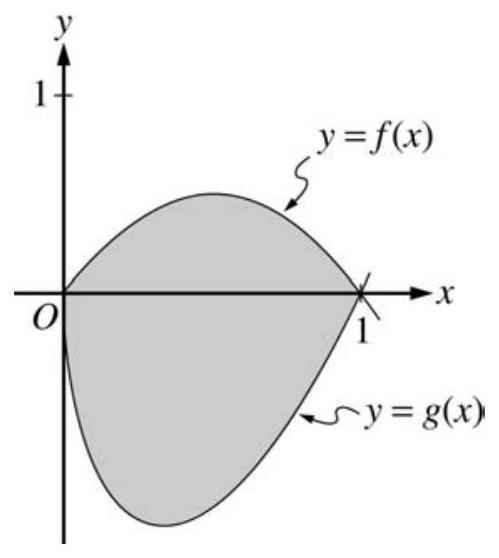
\includegraphics[width=0.6\linewidth]{figures/bc-2004_fig1.jpg}
\end{center}
Let $f$ and $g$ be the functions given by $f(x)=2 x(1-x)$ and $g(x)=3(x-1) \sqrt{x}$ for $0 \leq x \leq 1$. The graphs of $f$ and $g$ are shown in the figure above.\\
\begin{parts}
\part Find the area of the shaded region enclosed by the graphs of $f$ and $g$.
\part Find the volume of the solid generated when the shaded region enclosed by the graphs of $f$ and $g$ is revolved about the horizontal line $y=2$.
\part Let $h$ be the function given by $h(x)=k x(1-x)$ for $0 \leq x \leq 1$. For each $k>0$, the region (not shown) enclosed by the graphs of $h$ and $g$ is the base of a solid with square cross sections perpendicular to the $x$-axis. There is a value of $k$ for which the volume of this solid is equal to 15 . Write, but do not solve, an equation involving an integral expression that could be used to find the value of $k$.
\end{parts}
\begin{solution}
\begin{parts}
\part Area $=\int_{0}^{1}(f(x)-g(x)) d x$

\[=\int_{0}^{1}(2 x(1-x)-3(x-1) \sqrt{x}) d x=1.133\]
\part Volume $=\pi \int_{0}^{1}\left((2-g(x))^{2}-(2-f(x))^{2}\right) d x$\\
$=\pi \int_{0}^{1}\left((2-3(x-1) \sqrt{x})^{2}-(2-2 x(1-x))^{2}\right) d x$\\
$=16.179$
\end{parts}
\par\medskip
\textbf{Rubric:}\par
\begin{parts}
\part $2:\left\{\begin{array}{l}
1: \text { integral } \\
1: \text { answer }
\end{array}\right.$
\part $4:\left\{\begin{array}{l}1: \text { limits and constant } \\ 2: \text { integrand } \\ \quad\langle-1\rangle \text { each error } \\ \quad \text { Note: } 0 / 2 \text { if integral not of form } \\ \quad c \int_{a}^{b}\left(R^{2}(x)-r^{2}(x)\right) d x \\ 1: \text { answer }\end{array}\right.$
\part $3:\left\{\begin{array}{l}2: \text { integrand } \\ 1: \text { answer }\end{array}\right.$
\end{parts}
\end{solution}

\question
% Q3 | 2004 Calculus BC | Part A | Calculator Active
An object moving along a curve in the $x y$-plane has position $(x(t), y(t))$ at time $t \geq 0$ with $\frac{d x}{d t}=3+\cos \left(t^{2}\right)$. The derivative $\frac{d y}{d t}$ is not explicitly given. At time $t=2$, the object is at position $(1,8)$.\\
\begin{parts}
\part Find the $x$-coordinate of the position of the object at time $t=4$.
\part At time $t=2$, the value of $\frac{d y}{d t}$ is -7 . Write an equation for the line tangent to the curve at the point $(x(2), y(2))$.
\part Find the speed of the object at time $t=2$.
\part For $t \geq 3$, the line tangent to the curve at $(x(t), y(t))$ has a slope of $2 t+1$. Find the acceleration vector of the object at time $t=4$.
\end{parts}
\begin{solution}
\begin{parts}
\part $\quad x(4)=x(2)+\int_{2}^{4}\left(3+\cos \left(t^{2}\right)\right) d t$

\[=1+\int_{2}^{4}\left(3+\cos \left(t^{2}\right)\right) d t=7.132 \text { or } 7.133\]

(b)

\begin{align*}& \left.\frac{d y}{d x}\right|_{t=2}=\left.\frac{\frac{d y}{d t}}{\frac{d x}{d t}}\right|_{t=2}=\frac{-7}{3+\cos 4}=-2.983 \\
& y-8=-2.983(x-1)\end{align*}

$3:\left\{\begin{array}{l}1: \int_{2}^{4}\left(3+\cos \left(t^{2}\right)\right) d t \\ 1: \text { handles initial condition } \\ 1: \text { answer }\end{array}\right.$\\
$2:\left\{\begin{array}{l}1: \text { finds }\left.\frac{d y}{d x}\right|_{t=2} \\ 1: \text { equation }\end{array}\right.$
\part The speed of the object at time $t=2$ is $\sqrt{\left(x^{\prime}(2)\right)^{2}+\left(y^{\prime}(2)\right)^{2}}=7.382$ or 7.383.
\part $x^{\prime \prime}(4)=2.303$

\[\begin{aligned}
& y^{\prime}(t)=\frac{d y}{d t}=\frac{d y}{d x} \cdot \frac{d x}{d t}=(2 t+1)\left(3+\cos \left(t^{2}\right)\right) \\
& y^{\prime \prime}(4)=24.813 \text { or } 24.814
\end{aligned}\]
\end{parts}
\par\medskip
\textbf{Rubric:}\par
\begin{parts}
\part 1 : answer
\part $3:\left\{\begin{array}{l}
1: x^{\prime \prime}(4) \\
1: \frac{d y}{d t} \\
1: \text { answer }
\end{array}\right.$
\end{parts}
\end{solution}

\question
% Q4 | 2004 Calculus BC | Part B | Calculator Prohibited
Consider the curve given by $x^{2}+4 y^{2}=7+3 x y$.\\
\begin{parts}
\part Show that $\frac{d y}{d x}=\frac{3 y-2 x}{8 y-3 x}$.
\part Show that there is a point $P$ with $x$-coordinate 3 at which the line tangent to the curve at $P$ is horizontal. Find the $y$-coordinate of $P$.
\part Find the value of $\frac{d^{2} y}{d x^{2}}$ at the point $P$ found in part (b). Does the curve have a local maximum, a local minimum, or neither at the point $P$ ? Justify your answer.
\end{parts}
\begin{solution}
\begin{parts}
\part $\quad 2 x+8 y y^{\prime}=3 y+3 x y^{\prime}$

\begin{align*}(8 y-3 x) y^{\prime} & =3 y-2 x \\
y^{\prime} & =\frac{3 y-2 x}{8 y-3 x}\end{align*}
\part $\frac{3 y-2 x}{8 y-3 x}=0 ; 3 y-2 x=0$

When $x=3,3 y=6$

\[y=2\]

$3^{2}+4 \cdot 2^{2}=25$ and $7+3 \cdot 3 \cdot 2=25$\\
Therefore, $P=(3,2)$ is on the curve and the slope is 0 at this point.
\part $\frac{d^{2} y}{d x^{2}}=\frac{(8 y-3 x)\left(3 y^{\prime}-2\right)-(3 y-2 x)\left(8 y^{\prime}-3\right)}{(8 y-3 x)^{2}}$

At $P=(3,2), \frac{d^{2} y}{d x^{2}}=\frac{(16-9)(-2)}{(16-9)^{2}}=-\frac{2}{7}$.\\
Since $y^{\prime}=0$ and $y^{\prime \prime}<0$ at $P$, the curve has a local maximum at $P$.
\end{parts}
\par\medskip
\textbf{Rubric:}\par
\[\begin{aligned}
& 2:\left\{\begin{array}{l}
1: \text { implicit differentiation } \\
1: \text { solves for } y^{\prime}
\end{array}\right. \\
& 3:\left\{\begin{array}{l}
1: \frac{d y}{d x}=0 \\
1: \text { shows slope is } 0 \text { at }(3,2) \\
1: \text { shows }(3,2) \text { lies on curve }
\end{array}\right. \\
& 4:\left\{\begin{array}{l}
2: \frac{d^{2} y}{d x^{2}} \\
1: \text { value of } \frac{d^{2} y}{d x^{2}} \text { at }(3,2) \\
1: \text { conclusion with justification }
\end{array}\right.
\end{aligned}\]
\end{solution}

\question
% Q5 | 2004 Calculus BC | Part B | Calculator Prohibited
A population is modeled by a function $P$ that satisfies the logistic differential equation
\[\frac{d P}{d t}=\frac{P}{5}\left(1-\frac{P}{12}\right) .\]
\begin{parts}
\part If $P(0)=3$, what is $\lim _{t \rightarrow \infty} P(t)$ ?

If $P(0)=20$, what is $\lim _{t \rightarrow \infty} P(t)$ ?
\part If $P(0)=3$, for what value of $P$ is the population growing the fastest?
\part A different population is modeled by a function $Y$ that satisfies the separable differential equation

\[\frac{d Y}{d t}=\frac{Y}{5}\left(1-\frac{t}{12}\right)\]

Find $Y(t)$ if $Y(0)=3$.
\part For the function $Y$ found in part (c), what is $\lim _{t \rightarrow \infty} Y(t)$ ?
\end{parts}
\begin{solution}
\begin{parts}
\part For this logistic differential equation, the carrying capacity is 12 .

If $P(0)=3, \lim _{t \rightarrow \infty} P(t)=12$.\\
If $P(0)=20, \lim _{t \rightarrow \infty} P(t)=12$.
\part The population is growing the fastest when $P$ is half the carrying capacity. Therefore, $P$ is growing the fastest when $P=6$.
\part $\frac{1}{Y} d Y=\frac{1}{5}\left(1-\frac{t}{12}\right) d t=\left(\frac{1}{5}-\frac{t}{60}\right) d t$\\
$\ln |Y|=\frac{t}{5}-\frac{t^{2}}{120}+C$\\
$Y(t)=K e^{\frac{t}{5}-\frac{t^{2}}{120}}$\\
$K=3$\\
$Y(t)=3 e^{\frac{t}{5}-\frac{t^{2}}{120}}$
\part $\lim _{t \rightarrow \infty} Y(t)=0$
\end{parts}
\par\medskip
\textbf{Rubric:}\par
\begin{parts}
\part $2:\left\{\begin{array}{l}1: \text { answer } \\ 1: \text { answer }\end{array}\right.$
\part 1 : answer
\part $5:\left\{\begin{array}{l}1: \text { separates variables } \\ 1: \text { antiderivatives } \\ 1: \text { constant of integration } \\ 1: \text { uses initial condition } \\ 1: \text { solves for } Y \\ 0 / 1 \text { if } Y \text { is not exponential }\end{array}\right.$
\part Note: $\max 2 / 5[1-1-0-0-0]$ if no constant of integration
\part Note: $0 / 5$ if no separation of variables
\part 1 : answer
\end{parts}
\end{solution}

\question
% Q6 | 2004 Calculus BC | Part B | Calculator Prohibited
Let $f$ be the function given by $f(x)=\sin \left(5 x+\frac{\pi}{4}\right)$, and let $P(x)$ be the third-degree Taylor polynomial for $f$ about $x=0$.\\
\begin{parts}
\part Find $P(x)$.
\part Find the coefficient of $x^{22}$ in the Taylor series for $f$ about $x=0$.
\part Use the Lagrange error bound to show that $\left|f\left(\frac{1}{10}\right)-P\left(\frac{1}{10}\right)\right|<\frac{1}{100}$.
\part Let $G$ be the function given by $G(x)=\int_{0}^{x} f(t) d t$. Write the third-degree Taylor polynomial for $G$ about $x=0$.
\end{parts}
\begin{solution}
\begin{parts}
\part $f(0)=\sin \left(\frac{\pi}{4}\right)=\frac{\sqrt{2}}{2}$

\[\begin{aligned}
& f^{\prime}(0)=5 \cos \left(\frac{\pi}{4}\right)=\frac{5 \sqrt{2}}{2} \\
& f^{\prime \prime}(0)=-25 \sin \left(\frac{\pi}{4}\right)=-\frac{25 \sqrt{2}}{2} \\
& f^{\prime \prime \prime}(0)=-125 \cos \left(\frac{\pi}{4}\right)=-\frac{125 \sqrt{2}}{2} \\
& P(x)=\frac{\sqrt{2}}{2}+\frac{5 \sqrt{2}}{2} x-\frac{25 \sqrt{2}}{2(2!)} x^{2}-\frac{125 \sqrt{2}}{2(3!)} x^{3}
\end{aligned}\]
\part $\frac{-5^{22} \sqrt{2}}{2(22!)}$
\part $\left|f\left(\frac{1}{10}\right)-P\left(\frac{1}{10}\right)\right| \leq \max _{0 \leq c \leq \frac{1}{10}}\left|f^{(4)}(c)\right|\left(\frac{1}{4!}\right)\left(\frac{1}{10}\right)^{4}$

\[\leq \frac{625}{4!}\left(\frac{1}{10}\right)^{4}=\frac{1}{384}<\frac{1}{100}\]
\part The third-degree Taylor polynomial for $G$ about

\[\begin{aligned}
x=0 \text { is } & \int_{0}^{x}\left(\frac{\sqrt{2}}{2}+\frac{5 \sqrt{2}}{2} t-\frac{25 \sqrt{2}}{4} t^{2}\right) d t \\
& =\frac{\sqrt{2}}{2} x+\frac{5 \sqrt{2}}{4} x^{2}-\frac{25 \sqrt{2}}{12} x^{3}
\end{aligned}\]

4 : $P(x)$\\
$\langle-1\rangle$ each error or missing term deduct only once for $\sin \left(\frac{\pi}{4}\right)$ evaluation error\\
deduct only once for $\cos \left(\frac{\pi}{4}\right)$ evaluation error\\
$\langle-1\rangle$ max for all extra terms, $+\cdots$, misuse of equality
\end{parts}
\par\medskip
\textbf{Rubric:}\par
\begin{parts}
\part $2:\left\{\begin{array}{l}1: \text { magnitude } \\ 1: \text { sign }\end{array}\right.$
\part 1 : error bound in an appropriate inequality
\part 2 : third-degree Taylor polynomial for $G$ about $x=0$
\end{parts}
\end{solution}

\end{questions}

\section*{2004 AP Calculus BC Form B}

\begin{questions}

\question
% Q1 | 2004 Calculus BC Form B | Part A | Calculator Active
A particle moving along a curve in the plane has position $(x(t), y(t))$ at time $t$, where
\[\frac{d x}{d t}=\sqrt{t^{4}+9} \text { and } \frac{d y}{d t}=2 e^{t}+5 e^{-t}\]

for all real values of $t$. At time $t=0$, the particle is at the point $(4,1)$.\\
\begin{parts}
\part Find the speed of the particle and its acceleration vector at time $t=0$.
\part Find an equation of the line tangent to the path of the particle at time $t=0$.
\part Find the total distance traveled by the particle over the time interval $0 \leq t \leq 3$.
\part Find the $x$-coordinate of the position of the particle at time $t=3$.
\end{parts}
\begin{solution}
\begin{parts}
\part At time $t=0$ :

Speed $=\sqrt{x^{\prime}(0)^{2}+y^{\prime}(0)^{2}}=\sqrt{3^{2}+7^{2}}=\sqrt{58}$

Acceleration vector $=\left\langle x^{\prime \prime}(0), y^{\prime \prime}(0)\right\rangle=\langle 0,-3\rangle$
\part $\frac{d y}{d x}=\frac{y^{\prime}(0)}{x^{\prime}(0)}=\frac{7}{3}$

Tangent line is $y=\frac{7}{3}(x-4)+1$
\part Distance $=\int_{0}^{3} \sqrt{\left(\sqrt{t^{4}+9}\right)^{2}+\left(2 e^{t}+5 e^{-t}\right)^{2}} d t$

\[=45.226 \text { or } 45.227\]
\part $\quad x(3)=4+\int_{0}^{3} \sqrt{t^{4}+9} d t$

\[=17.930 \text { or } 17.931\]
\end{parts}
\par\medskip
\textbf{Rubric:}\par
\begin{parts}
\part $2:\left\{\begin{array}{l}
1: \text { speed } \\
1: \text { acceleration vector }
\end{array}\right.$
\part $2:\left\{\begin{array}{l}
1: \text { slope } \\
1: \text { tangent line }
\end{array}\right.$
\part $3:\left\{\begin{aligned}
2: & \text { distance integral } \\
& \langle-1\rangle \text { each integrand error } \\
& \langle-1\rangle \text { error in limits } \\
1: & \text { answer }
\end{aligned}\right.$
\part $2:\left\{\begin{array}{l}
1: \text { integral } \\
1: \text { answer }
\end{array}\right.$
\end{parts}
\end{solution}

\question
% Q2 | 2004 Calculus BC Form B | Part A | Calculator Active
Let $f$ be a function having derivatives of all orders for all real numbers. The third-degree Taylor polynomial for $f$ about $x=2$ is given by

\[T(x)=7-9(x-2)^{2}-3(x-2)^{3} .\]
\begin{parts}
\part Find $f$ (2) and $f^{\prime \prime}(2)$.
\part Is there enough information given to determine whether $f$ has a critical point at $x=2$ ?

If not, explain why not.\\
If so, determine whether $f(2)$ is a relative maximum, a relative minimum, or neither, and justify your answer.
\part Use $T(x)$ to find an approximation for $f(0)$. Is there enough information given to determine whether $f$ has a critical point at $x=0$ ?\\
If not, explain why not.\\
If so, determine whether $f(0)$ is a relative maximum, a relative minimum, or neither, and justify your answer.
\part The fourth derivative of $f$ satisfies the inequality $\left|f^{(4)}(x)\right| \leq 6$ for all $x$ in the closed interval [ 0,2 ]. Use the Lagrange error bound on the approximation to $f(0)$ found in part (c) to explain why $f(0)$ is negative.
\end{parts}
\begin{solution}
\begin{parts}
\part $f(2)=T(2)=7$\\
$\frac{f^{\prime \prime}(2)}{2!}=-9$ so $f^{\prime \prime}(2)=-18$
\part Yes, since $f^{\prime}(2)=T^{\prime}(2)=0, f$ does have a critical point at $x=2$.\\
Since $f^{\prime \prime}(2)=-18<0, f(2)$ is a relative maximum value.
\part $f(0) \approx T(0)=-5$

It is not possible to determine if $f$ has a critical point at $x=0$ because $T(x)$ gives exact information only at $x=2$.
\part Lagrange error bound $=\frac{6}{4!}|0-2|^{4}=4 f(0) \leq T(0)+4=-1$\\
Therefore, $f(0)$ is negative.
\end{parts}
\par\medskip
\textbf{Rubric:}\par
\begin{parts}
\part $2:\left\{\begin{array}{l}
1: f(2)=7 \\
1: f^{\prime \prime}(2)=-18
\end{array}\right.$
\part $2:\left\{\begin{aligned}
1 & : \text { states } f^{\prime}(2)=0 \\
1 & : \text { declares } f(2) \text { as a relative } \\
& \text { maximum because } f^{\prime \prime}(2)<0
\end{aligned}\right.$
\part $3:\left\{\begin{aligned}
1 & : f(0) \approx T(0)=-5 \\
1 & : \text { declares that it is not } \\
& \text { possible to determine } \\
1 & : \text { reason }
\end{aligned}\right.$
\part $2:\left\{\begin{aligned}
1: & \text { value of Lagrange error } \\
& \text { bound } \\
1: & \text { explanation }
\end{aligned}\right.$
\end{parts}
\end{solution}

\question
% Q3 | 2004 Calculus BC Form B | Part A | Calculator Active
\begin{center}
\begin{tabular}{|c|c|c|c|c|c|c|c|c|c|}
\hline
\begin{tabular}{c}
$t$ \\
(minutes) \\
\end{tabular} & 0 & 5 & 10 & 15 & 20 & 25 & 30 & 35 & 40 \\
\hline
\begin{tabular}{c}
$v(t)$ \\
(miles per minute) \\
\end{tabular} & 7.0 & 9.2 & 9.5 & 7.0 & 4.5 & 2.4 & 2.4 & 4.3 & 7.3 \\
\hline
\end{tabular}
\end{center}
A test plane flies in a straight line with positive velocity $v(t)$, in miles per minute at time $t$ minutes, where $v$ is a differentiable function of $t$. Selected values of $v(t)$ for $0 \leq t \leq 40$ are shown in the table above.\\
\begin{parts}
\part Use a midpoint Riemann sum with four subintervals of equal length and values from the table to approximate $\int_{0}^{40} v(t) d t$. Show the computations that lead to your answer. Using correct units, explain the meaning of $\int_{0}^{40} v(t) d t$ in terms of the plane's flight.
\part Based on the values in the table, what is the smallest number of instances at which the acceleration of the plane could equal zero on the open interval $0<t<40$ ? Justify your answer.
\part The function $f$, defined by $f(t)=6+\cos \left(\frac{t}{10}\right)+3 \sin \left(\frac{7 t}{40}\right)$, is used to model the velocity of the plane, in miles per minute, for $0 \leq t \leq 40$. According to this model, what is the acceleration of the plane at $t=23$ ? Indicate units of measure.
\part According to the model $f$, given in part (c), what is the average velocity of the plane, in miles per minute, over the time interval $0 \leq t \leq 40$ ?
\end{parts}
\begin{solution}
\begin{parts}
\part Midpoint Riemann sum is

\begin{align*}& 10 \cdot[v(5)+v(15)+v(25)+v(35)] \\
& =10 \cdot[9.2+7.0+2.4+4.3]=229\end{align*}

The integral gives the total distance in miles that the plane flies during the 40 minutes.
\part By the Mean Value Theorem, $v^{\prime}(t)=0$ somewhere in the interval $(0,15)$ and somewhere in the interval (25, 30). Therefore the acceleration will equal 0 for at least two values of $t$.
\part $f^{\prime}(23)=-0.407$ or -0.408 miles per minute ${ }^{2}$
\part Average velocity $=\frac{1}{40} \int_{0}^{40} f(t) d t$

\[=5.916 \text { miles per minute }\]
\end{parts}
\par\medskip
\textbf{Rubric:}\par
\begin{parts}
\part 1: v(5)+v(15)+v
\part $1 : answer with units$
\end{parts}
\end{solution}

\question
% Q4 | 2004 Calculus BC Form B | Part B | Calculator Prohibited
\begin{center}
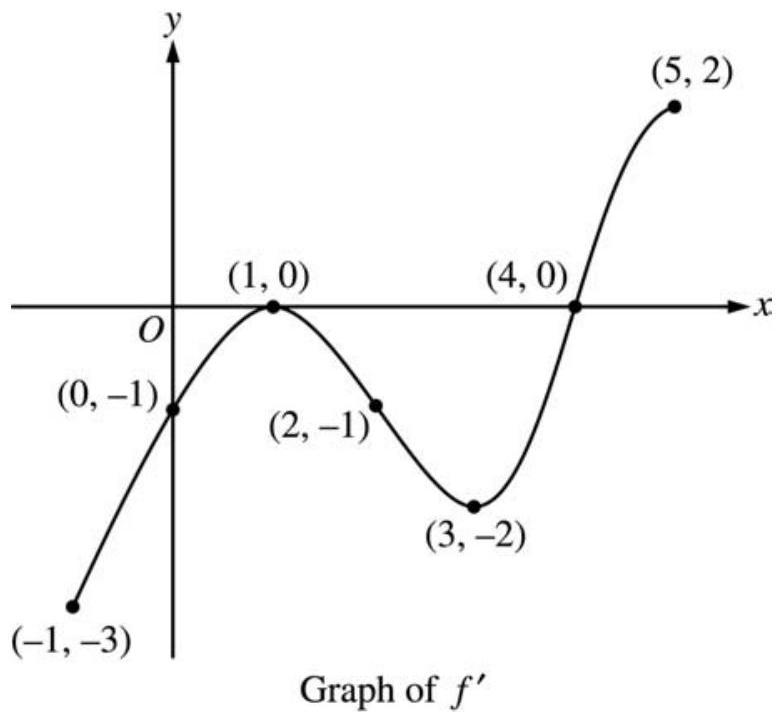
\includegraphics[width=0.6\linewidth]{figures/bc-2004-form-b_fig1.jpg}
\end{center}
The figure above shows the graph of $f^{\prime}$, the derivative of the function $f$, on the closed interval $-1 \leq x \leq 5$. The graph of $f^{\prime}$ has horizontal tangent lines at $x=1$ and $x=3$. The function $f$ is twice differentiable with $f(2)=6$.\\
\begin{parts}
\part Find the $x$-coordinate of each of the points of inflection of the graph of $f$. Give a reason for your answer.
\part At what value of $x$ does $f$ attain its absolute minimum value on the closed interval $-1 \leq x \leq 5$ ? At what value of $x$ does $f$ attain its absolute maximum value on the closed interval $-1 \leq x \leq 5$ ? Show the analysis that leads to your answers.
\part Let $g$ be the function defined by $g(x)=x f(x)$. Find an equation for the line tangent to the graph of $g$ at $x=2$.
\end{parts}
\begin{solution}
\begin{parts}
\part $\quad x=1$ and $x=3$ because the graph of $f^{\prime}$ changes from increasing to decreasing at $x=1$, and changes from decreasing to increasing at $x=3$.
\part The function $f$ decreases from $x=-1$ to $x=4$, then increases from $x=4$ to $x=5$.\\
Therefore, the absolute minimum value for $f$ is at $x=4$. The absolute maximum value must occur at $x=-1$ or at $x=5$.

\[f(5)-f(-1)=\int_{-1}^{5} f^{\prime}(t) d t<0\]

Since $f(5)<f(-1)$, the absolute maximum value occurs at $x=-1$.
\part $\quad g^{\prime}(x)=f(x)+x f^{\prime}(x)$\\
$g^{\prime}(2)=f(2)+2 f^{\prime}(2)=6+2(-1)=4$\\
$g(2)=2 f(2)=12$

Tangent line is $y=4(x-2)+12$
\end{parts}
\par\medskip
\textbf{Rubric:}\par
\begin{parts}
\part $2:\left\{\begin{array}{l}
1: x=1, x=3 \\
1: \text { reason }
\end{array}\right.$
\part $4:\left\{\begin{array}{l}1: \text { indicates } f \text { decreases then increases } \\ 1: \text { eliminates } x=5 \text { for maximum } \\ 1: \text { absolute minimum at } x=4 \\ 1: \text { absolute maximum at } x=-1\end{array}\right.$
\part $3:\left\{\begin{array}{l}2: g^{\prime}(x) \\ 1: \text { tangent line }\end{array}\right.$
\end{parts}
\end{solution}

\question
% Q5 | 2004 Calculus BC Form B | Part B | Calculator Prohibited
Let $g$ be the function given by $g(x)=\frac{1}{\sqrt{x}}$.\\
\begin{parts}
\part Find the average value of $g$ on the closed interval $[1,4]$.
\part Let $S$ be the solid generated when the region bounded by the graph of $y=g(x)$, the vertical lines $x=1$ and $x=4$, and the $x$-axis is revolved about the $x$-axis. Find the volume of $S$.
\part For the solid $S$, given in part (b), find the average value of the areas of the cross sections perpendicular to the $x$-axis.
\part The average value of a function $f$ on the unbounded interval $[a, \infty)$ is defined to be $\lim _{b \rightarrow \infty}\left[\frac{\int_{a}^{b} f(x) d x}{b-a}\right]$. Show that the improper integral $\int_{4}^{\infty} g(x) d x$ is divergent, but the average value of $g$ on the interval $[4, \infty)$ is finite.
\end{parts}
\begin{solution}
\begin{parts}
\part $\frac{1}{3} \int_{1}^{4} \frac{1}{\sqrt{x}} d x=\left.\frac{1}{3} \cdot 2 \sqrt{x}\right|_{1} ^{4}=\frac{4}{3}-\frac{2}{3}=\frac{2}{3}$

\[\begin{aligned}
& 2:\left\{\begin{array}{c}
1: \text { integral } \\
1: \text { antidifferentiation } \\
\text { and evaluation }
\end{array}\right. \\
& 2:\left\{\begin{array}{c}
1: \text { integral } \\
1: \text { antidifferentiation } \\
\text { and evaluation }
\end{array}\right.
\end{aligned}\]
\part The cross section at $x$ has area $\pi\left(\frac{1}{\sqrt{x}}\right)^{2}=\frac{\pi}{x}$

1 : answer\\
Average value $=\frac{1}{3} \int_{1}^{4} \frac{\pi}{x} d x=\frac{1}{3} \pi \ln 4$
\part $\quad \int_{4}^{\infty} g(x) d x=\lim _{b \rightarrow \infty} \int_{4}^{b} \frac{1}{\sqrt{x}} d x=\lim _{b \rightarrow \infty}(2 \sqrt{b}-4)=\infty$

This limit is not finite, so the integral is divergent.

\begin{align*}& \frac{\int_{4}^{b} g(x) d x}{b-4}=\frac{1}{b-4} \int_{4}^{b} \frac{1}{\sqrt{x}} d x=\frac{2 \sqrt{b}-4}{b-4} \\
& \lim _{b \rightarrow \infty} \frac{2 \sqrt{b}-4}{b-4}=0\end{align*}
\end{parts}
\par\medskip
\textbf{Rubric:}\par
\begin{parts}
\part $4:\left\{\begin{array}{l}
1: \int_{4}^{b} g(x) d x=2 \sqrt{b}-4 \\
1: \text { indicates integral diverges } \\
1: \frac{1}{b-4} \int_{4}^{b} g(x) d x=\frac{2 \sqrt{b}-4}{b-4} \\
1: \text { finite limit as } b \rightarrow \infty
\end{array}\right.$
\end{parts}
\end{solution}

\question
% Q6 | 2004 Calculus BC Form B | Part B | Calculator Prohibited
\begin{center}
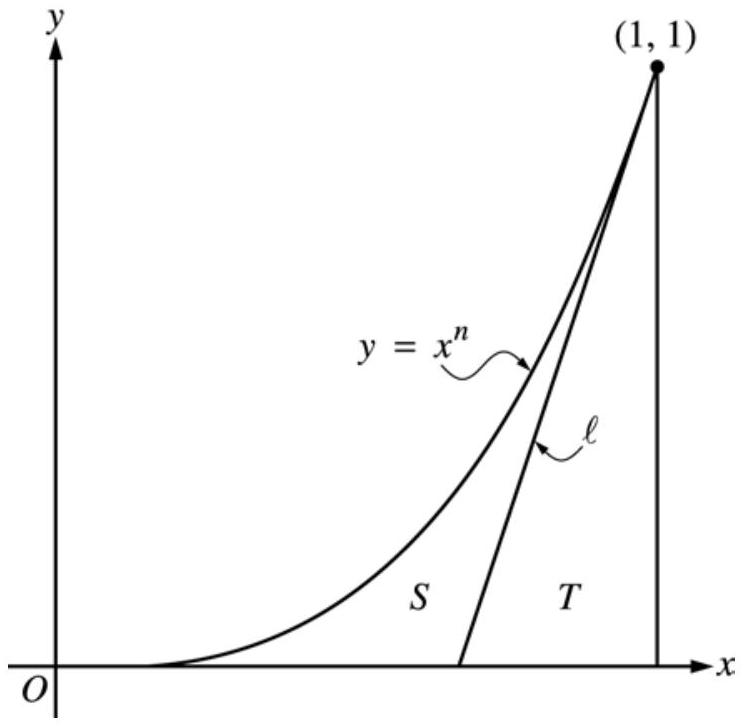
\includegraphics[width=0.6\linewidth]{figures/bc-2004-form-b_fig2.jpg}
\end{center}
Let $\ell$ be the line tangent to the graph of $y=x^{n}$ at the point $(1,1)$, where $n>1$, as shown above.\\
\begin{parts}
\part Find $\int_{0}^{1} x^{n} d x$ in terms of $n$.
\part Let $T$ be the triangular region bounded by $\ell$, the $x$-axis, and the line $x=1$. Show that the area of $T$ is $\frac{1}{2 n}$.
\part Let $S$ be the region bounded by the graph of $y=x^{n}$, the line $\ell$, and the $x$-axis. Express the area of $S$ in terms of $n$ and determine the value of $n$ that maximizes the area of $S$.
\end{parts}
\begin{solution}
\begin{parts}
\part $\quad \int_{0}^{1} x^{n} d x=\left.\frac{x^{n+1}}{n+1}\right|_{0} ^{1}=\frac{1}{n+1}$
\part Let $b$ be the length of the base of triangle $T$.\\
$\frac{1}{b}$ is the slope of line $\ell$, which is $n$\\
$\operatorname{Area}(T)=\frac{1}{2} b(1)=\frac{1}{2 n}$
\part $\quad \operatorname{Area}(S)=\int_{0}^{1} x^{n} d x-\operatorname{Area}(T)$

\[=\frac{1}{n+1}-\frac{1}{2 n}\]

$\frac{d}{d n} \operatorname{Area}(S)=-\frac{1}{(n+1)^{2}}+\frac{1}{2 n^{2}}=0$\\
$2 n^{2}=(n+1)^{2}$\\
$\sqrt{2} n=(n+1)$\\
$n=\frac{1}{\sqrt{2}-1}=1+\sqrt{2}$
\end{parts}
\par\medskip
\textbf{Rubric:}\par
\begin{parts}
\part $2:\left\{\begin{array}{l}1: \text { antiderivative of } x^{n} \\ 1: \text { answer }\end{array}\right.$
\part $3:\left\{\begin{array}{l}1: \text { slope of line } \ell \text { is } n \\ 1: \text { base of } T \text { is } \frac{1}{n} \\ 1: \text { shows area is } \frac{1}{2 n}\end{array}\right.$
\part $4:\left\{\begin{array}{l}1: \text { area of } S \text { in terms of } n \\ 1: \text { derivative } \\ 1: \text { sets derivative equal to } 0 \\ 1: \text { solves for } n\end{array}\right.$
\end{parts}
\end{solution}

\end{questions}

\section*{2005 AP Calculus BC}

\begin{questions}

\question
% Q1 | 2005 Calculus BC | Part A | Calculator Active
\begin{center}
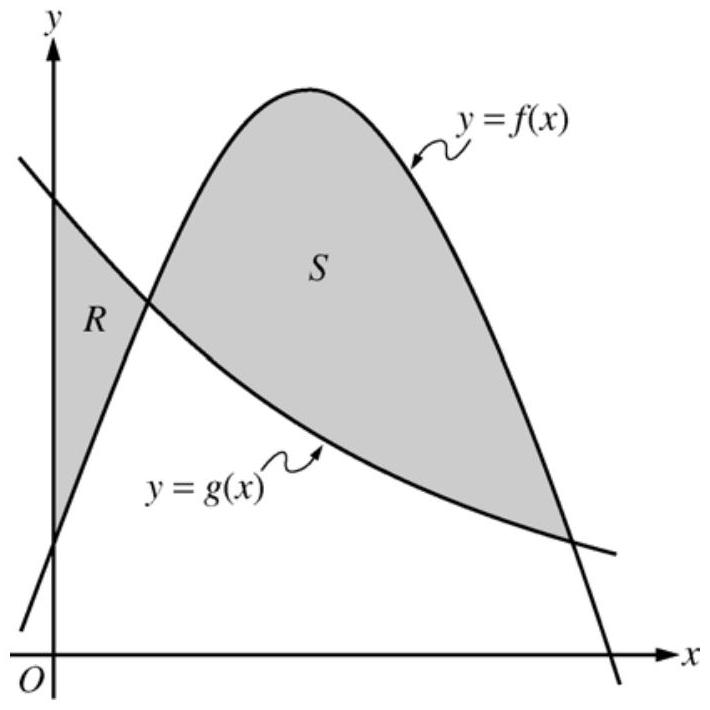
\includegraphics[width=0.6\linewidth]{figures/bc-2005_fig1.jpg}
\end{center}
Let $f$ and $g$ be the functions given by $f(x)=\frac{1}{4}+\sin (\pi x)$ and $g(x)=4^{-x}$. Let $R$ be the shaded region in the first quadrant enclosed by the $y$-axis and the graphs of $f$ and $g$, and let $S$ be the shaded region in the first quadrant enclosed by the graphs of $f$ and $g$, as shown in the figure above.\\
\begin{parts}
\part Find the area of $R$.
\part Find the area of $S$.
\part Find the volume of the solid generated when $S$ is revolved about the horizontal line $y=-1$.
\end{parts}
\begin{solution}
\begin{parts}
\part $\quad \int_{0}^{a}(g(x)-f(x)) d x=0.064$ or 0.065
\part $\quad \int_{a}^{1}(f(x)-g(x)) d x=0.410$
\part $\quad \pi \int_{a}^{1}\left((f(x)+1)^{2}-(g(x)+1)^{2}\right) d x=4.558$ or 4.559
\end{parts}
\par\medskip
\textbf{Rubric:}\par
\[\begin{aligned}
& 3:\left\{\begin{array}{l}
1: \text { limits } \\
1: \text { integrand } \\
1: \text { answer }
\end{array}\right. \\
& 3:\left\{\begin{array}{l}
1: \text { limits } \\
1: \text { integrand } \\
1: \text { answer }
\end{array}\right. \\
& 3:\left\{\begin{array}{l}
2: \text { integrand } \\
1: \text { limits, constant, and answer }
\end{array}\right.
\end{aligned}\]
\end{solution}

\question
% Q2 | 2005 Calculus BC | Part A | Calculator Active
\begin{center}
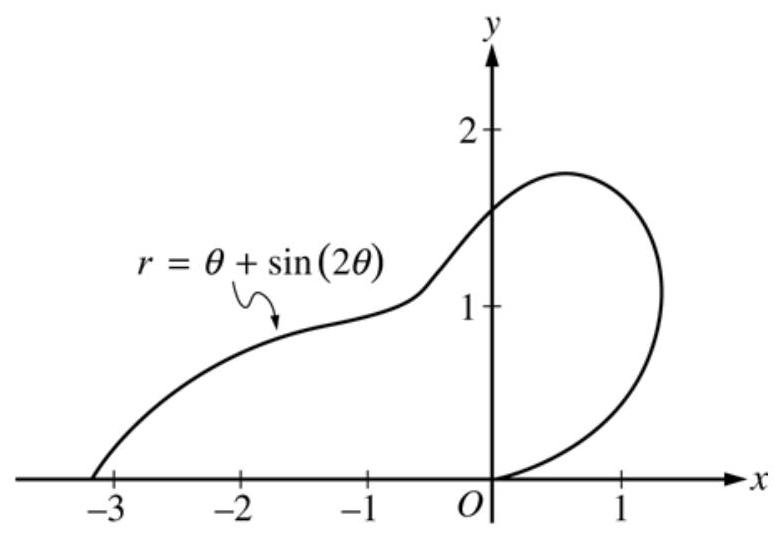
\includegraphics[width=0.6\linewidth]{figures/bc-2005_fig2.jpg}
\end{center}
The curve above is drawn in the $x y$-plane and is described by the equation in polar coordinates $r=\theta+\sin (2 \theta)$ for $0 \leq \theta \leq \pi$, where $r$ is measured in meters and $\theta$ is measured in radians. The derivative of $r$ with respect to $\theta$ is given by $\frac{d r}{d \theta}=1+2 \cos (2 \theta)$.\\
\begin{parts}
\part Find the area bounded by the curve and the $x$-axis.
\part Find the angle $\theta$ that corresponds to the point on the curve with $x$-coordinate -2 .
\part For $\frac{\pi}{3}<\theta<\frac{2 \pi}{3}, \frac{d r}{d \theta}$ is negative. What does this fact say about $r$ ? What does this fact say about the curve?
\part Find the value of $\theta$ in the interval $0 \leq \theta \leq \frac{\pi}{2}$ that corresponds to the point on the curve in the first quadrant with greatest distance from the origin. Justify your answer.
\end{parts}
\begin{solution}
\begin{parts}
\part Area $=\frac{1}{2} \int_{0}^{\pi} r^{2} d \theta$

\[=\frac{1}{2} \int_{0}^{\pi}(\theta+\sin (2 \theta))^{2} d \theta=4.382\]
\part $-2=r \cos (\theta)=(\theta+\sin (2 \theta)) \cos (\theta)$\\
$\theta=2.786$
\part Since $\frac{d r}{d \theta}<0$ for $\frac{\pi}{3}<\theta<\frac{2 \pi}{3}, r$ is decreasing on this interval. This means the curve is getting closer to the origin.
\part The only value in $\left[0, \frac{\pi}{2}\right]$ where $\frac{d r}{d \theta}=0$ is $\theta=\frac{\pi}{3}$.

\begin{center}
\begin{tabular}{|c|l|}
\hline
$\theta$ & \multicolumn{1}{|c|}{$r$} \\
\hline
0 & 0 \\
\hline
$\frac{\pi}{3}$ & 1.913 \\
\hline
$\frac{\pi}{2}$ & 1.571 \\
\hline
\end{tabular}
\end{center}

The greatest distance occurs when $\theta=\frac{\pi}{3}$.
\end{parts}
\par\medskip
\textbf{Rubric:}\par
\[\begin{aligned}
& 3:\left\{\begin{array}{l}
1: \text { limits and constant } \\
1: \text { integrand } \\
1: \text { answer }
\end{array}\right. \\
& 2:\left\{\begin{array}{l}
1: \text { equation } \\
1: \text { answer }
\end{array}\right. \\
& 2:\left\{\begin{array}{l}
1: \text { information about } r \\
1: \text { information about the curve }
\end{array}\right. \\
& 2:\left\{\begin{array}{l}
1: \theta=\frac{\pi}{3} \text { or } 1.047 \\
1: \text { answer with justification }
\end{array}\right.
\end{aligned}\]
\end{solution}

\question
% Q3 | 2005 Calculus BC | Part A | Calculator Active
\begin{center}
\begin{tabular}{|c||c|c|c|c|c|}
\hline
\begin{tabular}{c}
Distance \\
$x(\mathrm{~cm})$ \\
\end{tabular} & 0 & 1 & 5 & 6 & 8 \\
\hline
\begin{tabular}{c}
Temperature \\
$T(x)\left({ }^{\circ} \mathrm{C}\right)$ \\
\end{tabular} & 100 & 93 & 70 & 62 & 55 \\
\hline
\end{tabular}
\end{center}
A metal wire of length 8 centimeters (cm) is heated at one end. The table above gives selected values of the temperature $T(x)$, in degrees Celsius $\left({ }^{\circ} \mathrm{C}\right)$, of the wire $x \mathrm{~cm}$ from the heated end. The function $T$ is decreasing and twice differentiable.\\
\begin{parts}
\part Estimate $T^{\prime}(7)$. Show the work that leads to your answer. Indicate units of measure.
\part Write an integral expression in terms of $T(x)$ for the average temperature of the wire. Estimate the average temperature of the wire using a trapezoidal sum with the four subintervals indicated by the data in the table. Indicate units of measure.
\part Find $\int_{0}^{8} T^{\prime}(x) d x$, and indicate units of measure. Explain the meaning of $\int_{0}^{8} T^{\prime}(x) d x$ in terms of the temperature of the wire.
\part Are the data in the table consistent with the assertion that $T^{\prime \prime}(x)>0$ for every $x$ in the interval $0<x<8$ ? Explain your answer.
\end{parts}
\begin{solution}
\begin{parts}
\part $\frac{T(8)-T(6)}{8-6}=\frac{55-62}{2}=-\frac{7}{2}{ }^{\circ} \mathrm{C} / \mathrm{cm}$
\part $\frac{1}{8} \int_{0}^{8} T(x) d x$

Trapezoidal approximation for $\int_{0}^{8} T(x) d x$ :\\
$A=\frac{100+93}{2} \cdot 1+\frac{93+70}{2} \cdot 4+\frac{70+62}{2} \cdot 1+\frac{62+55}{2} \cdot 2$\\
Average temperature $\approx \frac{1}{8} A=75.6875^{\circ} \mathrm{C}$
\part $\quad \int_{0}^{8} T^{\prime}(x) d x=T(8)-T(0)=55-100=-45^{\circ} \mathrm{C}$

The temperature drops $45^{\circ} \mathrm{C}$ from the heated end of the wire to the other end of the wire.
\part Average rate of change of temperature on $[1,5]$ is $\frac{70-93}{5-1}=-5.75$. Average rate of change of temperature on $[5,6]$ is $\frac{62-70}{6-5}=-8$. No. By the MVT, $T^{\prime}\left(c_{1}\right)=-5.75$ for some $c_{1}$ in the interval $(1,5)$ and $T^{\prime}\left(c_{2}\right)=-8$ for some $c_{2}$ in the interval (5, 6). It follows that $T^{\prime}$ must decrease somewhere in the interval $\left(c_{1}, c_{2}\right)$. Therefore $T^{\prime \prime}$ is not positive for every $x$ in $[0,8]$.

Units of ${ }^{\circ} \mathrm{C} / \mathrm{cm}$ in (a), and ${ }^{\circ} \mathrm{C}$ in (b) and (c)
\end{parts}
\par\medskip
\textbf{Rubric:}\par
\begin{parts}
\part 1 : answer
\part $3:\left\{\begin{array}{l}1: \frac{1}{8} \int_{0}^{8} T(x) d x \\ 1: \text { trapezoidal sum } \\ 1: \text { answer }\end{array}\right.$
\part $2:\left\{\begin{array}{l}1: \text { value } \\ 1: \text { meaning }\end{array}\right.$
\part $2:\left\{\begin{array}{l}1: \text { two slopes of secant lines } \\ 1: \text { answer with explanation }\end{array}\right.$
\part 1 : units in (a), (b), and (c)
\end{parts}
\end{solution}

\question
% Q4 | 2005 Calculus BC | Part B | Calculator Prohibited
Consider the differential equation $\frac{d y}{d x}=2 x-y$.\\
\begin{parts}
\part On the axes provided, sketch a slope field for the given differential equation at the twelve points indicated, and sketch the solution curve that passes through the point $(0,1)$.\\
\begin{center}
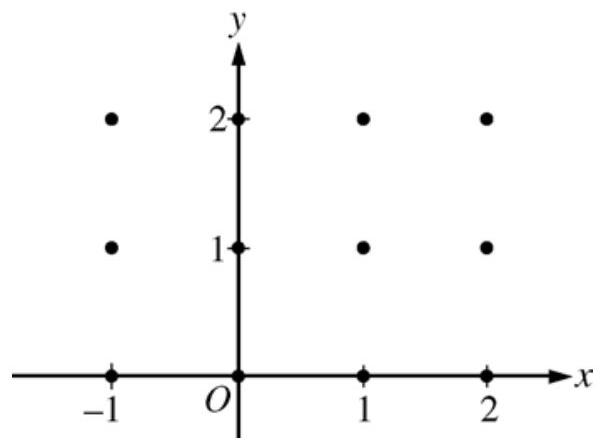
\includegraphics[width=0.6\linewidth]{figures/bc-2005_fig3.jpg}
\end{center}
\part The solution curve that passes through the point $(0,1)$ has a local minimum at $x=\ln \left(\frac{3}{2}\right)$. What is the $y$-coordinate of this local minimum?
\part Let $y=f(x)$ be the particular solution to the given differential equation with the initial condition $f(0)=1$. Use Euler's method, starting at $x=0$ with two steps of equal size, to approximate $f(-0.4)$. Show the work that leads to your answer.
\part Find $\frac{d^{2} y}{d x^{2}}$ in terms of $x$ and $y$. Determine whether the approximation found in part (c) is less than or greater than $f(-0.4)$. Explain your reasoning.
\end{parts}
\begin{solution}
(a)\\
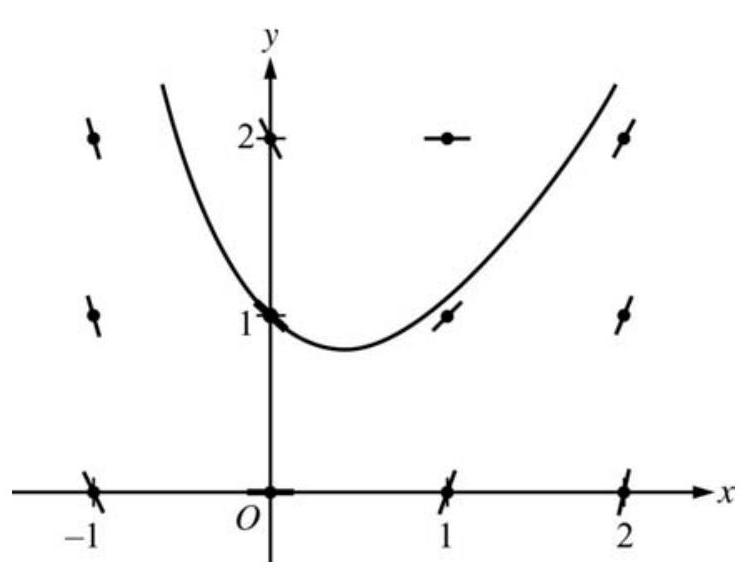
\includegraphics[width=0.6\linewidth]{figures/sg-bc-2005_fig4.jpg}

\[3:\left\{\begin{array}{l}
1: \text { zero slopes } \\
1: \text { nonzero slopes } \\
1: \text { curve through }(0,1)
\end{array}\right.\]
\begin{parts}
\part $\frac{d y}{d x}=0$ when $2 x=y$

The $y$-coordinate is $2 \ln \left(\frac{3}{2}\right)$.
\part $f(-0.2) \approx f(0)+f^{\prime}(0)(-0.2)$

\begin{align*}& =1+(-1)(-0.2)=1.2 \\
f(-0.4) & \approx f(-0.2)+f^{\prime}(-0.2)(-0.2) \\
& \approx 1.2+(-1.6)(-0.2)=1.52\end{align*}

$2:\left\{\begin{array}{l}1: \text { sets } \frac{d y}{d x}=0 \\ 1: \text { answer }\end{array}\right.$\\
$2:\left\{\begin{array}{l}1: \text { Euler's method with two steps } \\ 1: \text { Euler approximation to } f(-0.4)\end{array}\right.$
\part $\frac{d^{2} y}{d x^{2}}=2-\frac{d y}{d x}=2-2 x+y$\\
$\frac{d^{2} y}{d x^{2}}$ is positive in quadrant II because $x<0$ and $y>0$. $1.52<f(-0.4)$ since all solution curves in quadrant II are concave up.
\end{parts}
\end{solution}

\question
% Q5 | 2005 Calculus BC | Part B | Calculator Prohibited
\begin{center}
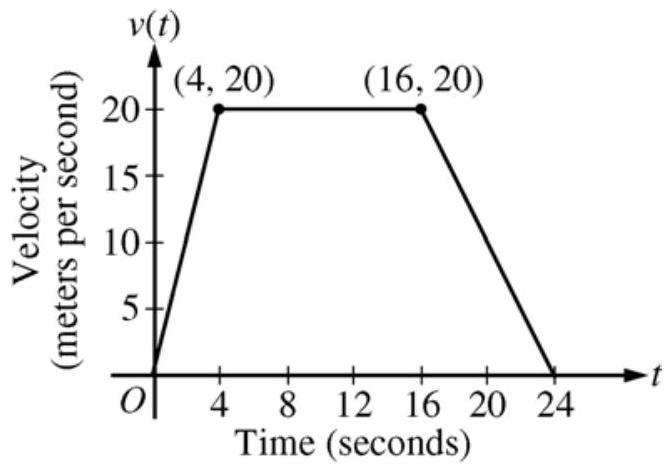
\includegraphics[width=0.6\linewidth]{figures/bc-2005_fig4.jpg}
\end{center}
A car is traveling on a straight road. For $0 \leq t \leq 24$ seconds, the car's velocity $v(t)$, in meters per second, is modeled by the piecewise-linear function defined by the graph above.\\
\begin{parts}
\part Find $\int_{0}^{24} v(t) d t$. Using correct units, explain the meaning of $\int_{0}^{24} v(t) d t$.
\part For each of $v^{\prime}(4)$ and $v^{\prime}(20)$, find the value or explain why it does not exist. Indicate units of measure.
\part Let $a(t)$ be the car's acceleration at time $t$, in meters per second per second. For $0<t<24$, write a piecewise-defined function for $a(t)$.
\part Find the average rate of change of $v$ over the interval $8 \leq t \leq 20$. Does the Mean Value Theorem guarantee a value of $c$, for $8<c<20$, such that $v^{\prime}(c)$ is equal to this average rate of change? Why or why not?
\end{parts}
\begin{solution}
\begin{parts}
\part $\quad \int_{0}^{24} v(t) d t=\frac{1}{2}(4)(20)+(12)(20)+\frac{1}{2}(8)(20)=360$

The car travels 360 meters in these 24 seconds.
\part $v^{\prime}(4)$ does not exist because

\[\begin{aligned}
& \lim _{t \rightarrow 4^{-}}\left(\frac{v(t)-v(4)}{t-4}\right)=5 \neq 0=\lim _{t \rightarrow 4^{+}}\left(\frac{v(t)-v(4)}{t-4}\right) \\
& v^{\prime}(20)=\frac{20-0}{16-24}=-\frac{5}{2} \mathrm{~m} / \mathrm{sec}^{2}
\end{aligned}\]
\part $a(t)=\left\{\begin{aligned} 5 & \text { if } 0<t<4 \\ 0 & \text { if } 4<t<16 \\ -\frac{5}{2} & \text { if } 16<t<24\end{aligned}\right.$\\
$a(t)$ does not exist at $t=4$ and $t=16$.
\part The average rate of change of $v$ on [8,20] is $\frac{v(20)-v(8)}{20-8}=-\frac{5}{6} \mathrm{~m} / \mathrm{sec}^{2}$.\\
No, the Mean Value Theorem does not apply to $v$ on [8, 20] because $v$ is not differentiable at $t=16$.
\end{parts}
\par\medskip
\textbf{Rubric:}\par
\begin{parts}
\part $2:\left\{\begin{array}{l}
1: \text { value } \\
1: \text { meaning with units }
\end{array}\right.$
\part $3:\left\{\begin{array}{l}1: v^{\prime}(4) \text { does not exist, with explanation } \\ 1: v^{\prime}(20) \\ 1: \text { units }\end{array}\right.$
\part $2:\left\{\begin{array}{l}1: \text { finds the values } 5,0,-\frac{5}{2} \\ 1: \text { identifies constants with correct intervals }\end{array}\right.$
\part $2:\left\{\begin{array}{l}1: \text { average rate of change of } v \text { on }[8,20] \\ 1: \text { answer with explanation }\end{array}\right.$
\end{parts}
\end{solution}

\question
% Q6 | 2005 Calculus BC | Part B | Calculator Prohibited
Let $f$ be a function with derivatives of all orders and for which $f(2)=7$. When $n$ is odd, the $n$th derivative of $f$ at $x=2$ is 0 . When $n$ is even and $n \geq 2$, the $n$th derivative of $f$ at $x=2$ is given by $f^{(n)}(2)=\frac{(n-1)!}{3^{n}}$.\\
\begin{parts}
\part Write the sixth-degree Taylor polynomial for $f$ about $x=2$.
\part In the Taylor series for $f$ about $x=2$, what is the coefficient of $(x-2)^{2 n}$ for $n \geq 1$ ?
\part Find the interval of convergence of the Taylor series for $f$ about $x=2$. Show the work that leads to your answer.
\end{parts}
\begin{solution}
\begin{parts}
\part $\quad P_{6}(x)=7+\frac{1!}{3^{2}} \cdot \frac{1}{2!}(x-2)^{2}+\frac{3!}{3^{4}} \cdot \frac{1}{4!}(x-2)^{4}+\frac{5!}{3^{6}} \cdot \frac{1}{6!}(x-2)^{6}$

\[3:\left\{\begin{aligned}
1 & : \text { polynomial about } x=2 \\
2 & : P_{6}(x) \\
& \langle-1\rangle \text { each incorrect term } \\
& \langle-1\rangle \text { max for all extra terms, } \\
& \quad+\cdots, \text { misuse of equality }
\end{aligned}\right.\]
\part $\frac{(2 n-1)!}{3^{2 n}} \cdot \frac{1}{(2 n)!}=\frac{1}{3^{2 n}(2 n)}$

1 : coefficient
\part The Taylor series for $f$ about $x=2$ is

\begin{align*}f(x) & =7+\sum_{n=1}^{\infty} \frac{1}{2 n \cdot 3^{2 n}}(x-2)^{2 n} . \\
L & =\lim _{n \rightarrow \infty}\left|\frac{\frac{1}{2(n+1)} \cdot \frac{1}{3^{2(n+1)}}(x-2)^{2(n+1)}}{\frac{1}{2 n} \cdot \frac{1}{3^{2 n}}(x-2)^{2 n}}\right| \\
& =\lim _{n \rightarrow \infty}\left|\frac{2 n}{2(n+1)} \cdot \frac{3^{2 n}}{3^{2} 3^{2 n}}(x-2)^{2}\right|=\frac{(x-2)^{2}}{9} \\
L & <1 \text { when }|x-2|<3\end{align*}

Thus, the series converges when $-1<x<5$.\\
When $x=5$, the series is $7+\sum_{n=1}^{\infty} \frac{3^{2 n}}{2 n \cdot 3^{2 n}}=7+\frac{1}{2} \sum_{n=1}^{\infty} \frac{1}{n}$,\\
which diverges, because $\sum_{n=1}^{\infty} \frac{1}{n}$, the harmonic series, diverges.\\
When $x=-1$, the series is $7+\sum_{n=1}^{\infty} \frac{(-3)^{2 n}}{2 n \cdot 3^{2 n}}=7+\frac{1}{2} \sum_{n=1}^{\infty} \frac{1}{n}$,\\
which diverges, because $\sum_{n=1}^{\infty} \frac{1}{n}$, the harmonic series, diverges.\\
The interval of convergence is $(-1,5)$.
\end{parts}
\par\medskip
\textbf{Rubric:}\par
\begin{parts}
\part $5:\left\{\begin{array}{l}
1: \text { sets up ratio } \\
1: \text { computes limit of ratio } \\
1: \text { identifies interior of } \\
\quad \text { interval of convergence } \\
1: \text { considers both endpoints } \\
1: \text { analysis/conclusion for } \\
\quad \text { both endpoints }
\end{array}\right.$
\end{parts}
\end{solution}

\end{questions}

\section*{2005 AP Calculus BC Form B}

\begin{questions}

\question
% Q1 | 2005 Calculus BC Form B | Part A | Calculator Active
An object moving along a curve in the $x y$-plane has position $(x(t), y(t))$ at time $t \geq 0$ with
\[\frac{d x}{d t}=12 t-3 t^{2} \text { and } \frac{d y}{d t}=\ln \left(1+(t-4)^{4}\right)\]

At time $t=0$, the object is at position $(-13,5)$. At time $t=2$, the object is at point $P$ with $x$-coordinate 3 .\\
\begin{parts}
\part Find the acceleration vector at time $t=2$ and the speed at time $t=2$.
\part Find the $y$-coordinate of $P$.
\part Write an equation for the line tangent to the curve at $P$.
\part For what value of $t$, if any, is the object at rest? Explain your reasoning.
\end{parts}
\begin{solution}
\begin{parts}
\part $x^{\prime \prime}(2)=0, y^{\prime \prime}(2)=-\frac{32}{17}=-1.882$

\begin{align*}& a(2)=\langle 0,-1.882\rangle \\
& \text { Speed }=\sqrt{12^{2}+(\ln (17))^{2}}=12.329 \text { or } 12.330\end{align*}
\part $y(t)=y(0)+\int_{0}^{t} \ln \left(1+(u-4)^{4}\right) d u$

\[y(2)=5+\int_{0}^{2} \ln \left(1+(u-4)^{4}\right) d u=13.671\]
\part At $t=2$, slope $=\frac{\frac{d y}{d t}}{\frac{d x}{d t}}=\frac{\ln (17)}{12}=0.236 y-13.671=0.236(x-3)$
\part $\quad x^{\prime}(t)=0$ if $t=0,4$\\
$y^{\prime}(t)=0$ if $t=4$
\end{parts}
\par\medskip
\textbf{Rubric:}\par
\begin{parts}
\part $2:\left\{\begin{array}{l}
1: \text { acceleration vector } \\
1: \text { speed }
\end{array}\right.$
\part $3:\left\{\begin{array}{l}
1: \int_{0}^{2} \ln \left(1+(u-4)^{4}\right) d u \\
1: \text { handles initial condition } \\
1: \text { answer }
\end{array}\right.$
\part $2:\left\{\begin{array}{l}
1: \text { slope } \\
1: \text { equation }
\end{array}\right.$
\part $2:\left\{\begin{array}{l}
1: \text { reason } \\
1: \text { answer }
\end{array}\right.$
\end{parts}
\end{solution}

\question
% Q2 | 2005 Calculus BC Form B | Part A | Calculator Active
A water tank at Camp Newton holds 1200 gallons of water at time $t=0$. During the time interval $0 \leq t \leq 18$ hours, water is pumped into the tank at the rate
\[W(t)=95 \sqrt{t} \sin ^{2}\left(\frac{t}{6}\right) \text { gallons per hour. }\]

During the same time interval, water is removed from the tank at the rate

\[R(t)=275 \sin ^{2}\left(\frac{t}{3}\right) \text { gallons per hour. }\]
\begin{parts}
\part Is the amount of water in the tank increasing at time $t=15$ ? Why or why not?
\part To the nearest whole number, how many gallons of water are in the tank at time $t=18$ ?
\part At what time $t$, for $0 \leq t \leq 18$, is the amount of water in the tank at an absolute minimum? Show the work that leads to your conclusion.
\part For $t>18$, no water is pumped into the tank, but water continues to be removed at the rate $R(t)$ until the tank becomes empty. Let $k$ be the time at which the tank becomes empty. Write, but do not solve, an equation involving an integral expression that can be used to find the value of $k$.
\end{parts}
\begin{solution}
\begin{parts}
\part No; the amount of water is not increasing at $t=15$ 1 : answer with reason since $W(15)-R(15)=-121.09<0$.
\part $\quad 1200+\int_{0}^{18}(W(t)-R(t)) d t=1309.788$ 1310 gallons

\[\begin{aligned}
& 3:\left\{\begin{array}{l}
1: \text { limits } \\
1: \text { integrand } \\
1: \text { answer }
\end{array}\right. \\
& 3:\left\{\begin{array}{l}
1: \text { interior critical points } \\
1: \text { amount of water is least at } \\
t=6.494 \text { or } 6.495 \\
1: \text { analysis for absolute minimum }
\end{array}\right.
\end{aligned}\]

The values at the endpoints and the critical points show that the absolute minimum occurs when $t=6.494$ or 6.495 .
\part $\quad \int_{18}^{k} R(t) d t=1310$
\end{parts}
\par\medskip
\textbf{Rubric:}\par
\begin{parts}
\part $2:\left\{\begin{array}{l}
1: \text { limits } \\
1: \text { equation }
\end{array}\right.$
\end{parts}
\end{solution}

\question
% Q3 | 2005 Calculus BC Form B | Part A | Calculator Active
The Taylor series about $x=0$ for a certain function $f$ converges to $f(x)$ for all $x$ in the interval of convergence. The $n$th derivative of $f$ at $x=0$ is given by
\[f^{(n)}(0)=\frac{(-1)^{n+1}(n+1)!}{5^{n}(n-1)^{2}} \text { for } n \geq 2\]

The graph of $f$ has a horizontal tangent line at $x=0$, and $f(0)=6$.\\
\begin{parts}
\part Determine whether $f$ has a relative maximum, a relative minimum, or neither at $x=0$. Justify your answer.
\part Write the third-degree Taylor polynomial for $f$ about $x=0$.
\part Find the radius of convergence of the Taylor series for $f$ about $x=0$. Show the work that leads to your answer.
\end{parts}
\begin{solution}
\begin{parts}
\part $f$ has a relative maximum at $x=0$ because\\
$f^{\prime}(0)=0$ and $f^{\prime \prime}(0)<0$.

\[2:\left\{\begin{array}{l}
1: \text { answer } \\
1: \text { reason }
\end{array}\right.\]
\part $\quad f(0)=6, f^{\prime}(0)=0$

\begin{align*}& f^{\prime \prime}(0)=-\frac{3!}{5^{2} 1^{2}}=-\frac{6}{25}, f^{\prime \prime \prime}(0)=\frac{4!}{5^{3} 2^{2}} \\
& P(x)=6-\frac{3!x^{2}}{5^{2} 2!}+\frac{4!x^{3}}{5^{3} 2^{2} 3!}=6-\frac{3}{25} x^{2}+\frac{1}{125} x^{3}\end{align*}

\begin{align*}3: & P(x) \\
& \langle-1\rangle \text { each incorrect term }\end{align*}

Note: $\langle-1\rangle$ max for use of extra terms

\[4:\left\{\begin{array}{l}
1: \text { general term } \\
1: \text { sets up ratio } \\
1: \text { computes limit } \\
1: \text { applies ratio test to get } \\
\text { radius of convergence }
\end{array}\right.\]
\part $u_{n}=\frac{f^{(n)}(0)}{n!} x^{n}=\frac{(-1)^{n+1}(n+1)}{5^{n}(n-1)^{2}} x^{n}$

\[\begin{aligned}
& \begin{aligned}
&\left|\frac{u_{n+1}}{u_{n}}\right|=\left|\frac{\frac{(-1)^{n+2}(n+2)}{5^{n+1} n^{2}} x^{n+1}}{\frac{(-1)^{n+1}(n+1)}{5^{n}(n-1)^{2}} x^{n}}\right| \\
&=\left(\frac{n+2}{n+1}\right)\left(\frac{n-1}{n}\right)^{2} \frac{1}{5}|x| \\
& \lim _{n \rightarrow \infty}\left|\frac{u_{n+1}}{u_{n}}\right|=\frac{1}{5}|x|<1 \text { if }|x|<5
\end{aligned}
\end{aligned}\]

The radius of convergence is 5 .
\end{parts}
\end{solution}

\question
% Q4 | 2005 Calculus BC Form B | Part B | Calculator Prohibited
\begin{center}
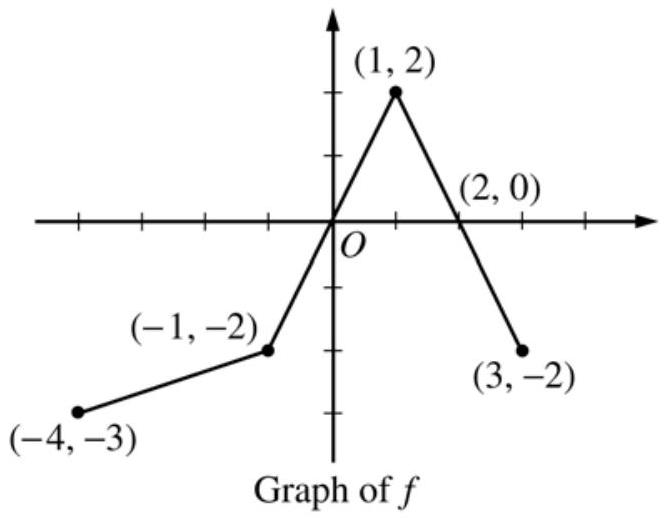
\includegraphics[width=0.6\linewidth]{figures/bc-2005-form-b_fig1.jpg}
\end{center}
The graph of the function $f$ above consists of three line segments.\\
\begin{parts}
\part Let $g$ be the function given by $g(x)=\int_{-4}^{x} f(t) d t$. For each of $g(-1), g^{\prime}(-1)$, and $g^{\prime \prime}(-1)$, find the value or state that it does not exist.
\part For the function $g$ defined in part (a), find the $x$-coordinate of each point of inflection of the graph of $g$ on the open interval $-4<x<3$. Explain your reasoning.
\part Let $h$ be the function given by $h(x)=\int_{x}^{3} f(t) d t$. Find all values of $x$ in the closed interval $-4 \leq x \leq 3$ for which $h(x)=0$.
\part For the function $h$ defined in part (c), find all intervals on which $h$ is decreasing. Explain your reasoning.
\end{parts}
\begin{solution}
\begin{parts}
\part $\quad g(-1)=\int_{-4}^{-1} f(t) d t=-\frac{1}{2}(3)(5)=-\frac{15}{2}$\\
$g^{\prime}(-1)=f(-1)=-2$\\
$g^{\prime \prime}(-1)$ does not exist because $f$ is not differentiable at $x=-1$.
\part $x=1$\\
$g^{\prime}=f$ changes from increasing to decreasing at $x=1$.
\part $x=-1,1,3$
\part $h$ is decreasing on $[0,2]$
\end{parts}
\par\medskip
\textbf{Rubric:}\par
\begin{parts}
\part $3:\left\{\begin{array}{l}
1: g(-1) \\
1: g^{\prime}(-1) \\
1: g^{\prime \prime}(-1)
\end{array}\right.$
\part $2:\left\{\begin{array}{l}
1: x=1 \text { (only) } \\
1: \text { reason }
\end{array}\right.$
\part 2 : correct values
\part $2:\left\{\begin{array}{l}
1: \text { interval } \\
1: \text { reason }
\end{array}\right.$
\end{parts}
\end{solution}

\question
% Q5 | 2005 Calculus BC Form B | Part B | Calculator Prohibited
Consider the curve given by $y^{2}=2+x y$.\\
\begin{parts}
\part Show that $\frac{d y}{d x}=\frac{y}{2 y-x}$.
\part Find all points $(x, y)$ on the curve where the line tangent to the curve has slope $\frac{1}{2}$.
\part Show that there are no points $(x, y)$ on the curve where the line tangent to the curve is horizontal.
\part Let $x$ and $y$ be functions of time $t$ that are related by the equation $y^{2}=2+x y$. At time $t=5$, the value of $y$ is 3 and $\frac{d y}{d t}=6$. Find the value of $\frac{d x}{d t}$ at time $t=5$.
\end{parts}
\begin{solution}
\begin{parts}
\part $2 y y^{\prime}=y+x y^{\prime}$\\
$(2 y-x) y^{\prime}=y$\\
$y^{\prime}=\frac{y}{2 y-x}$
\part $\frac{y}{2 y-x}=\frac{1}{2}$\\
$2 y=2 y-x$\\
$x=0$\\
$y= \pm \sqrt{2}$\\
$(0, \sqrt{2}),(0,-\sqrt{2})$\\
$2:\left\{\begin{array}{l}1: \text { implicit differentiation } \\ 1: \text { solves for } y^{\prime}\end{array}\right.$\\
$2:\left\{\begin{array}{l}1: \frac{y}{2 y-x}=\frac{1}{2} \\ 1: \text { answer }\end{array}\right.$
\part $\frac{y}{2 y-x}=0$\\
$y=0$\\
The curve has no horizontal tangent since\\
$0^{2} \neq 2+x \cdot 0$ for any $x$.
\part When $y=3,3^{2}=2+3 x$ so $x=\frac{7}{3}$.\\
$\frac{d y}{d t}=\frac{d y}{d x} \cdot \frac{d x}{d t}=\frac{y}{2 y-x} \cdot \frac{d x}{d t}$
\end{parts}
\par\medskip
\textbf{Rubric:}\par
\begin{parts}
\part $3:\left\{\begin{array}{l}
1: \text { solves for } x \\
1: \text { chain rule } \\
1: \text { answer }
\end{array}\right.$
\end{parts}
\end{solution}

\question
% Q6 | 2005 Calculus BC Form B | Part B | Calculator Prohibited
\begin{center}
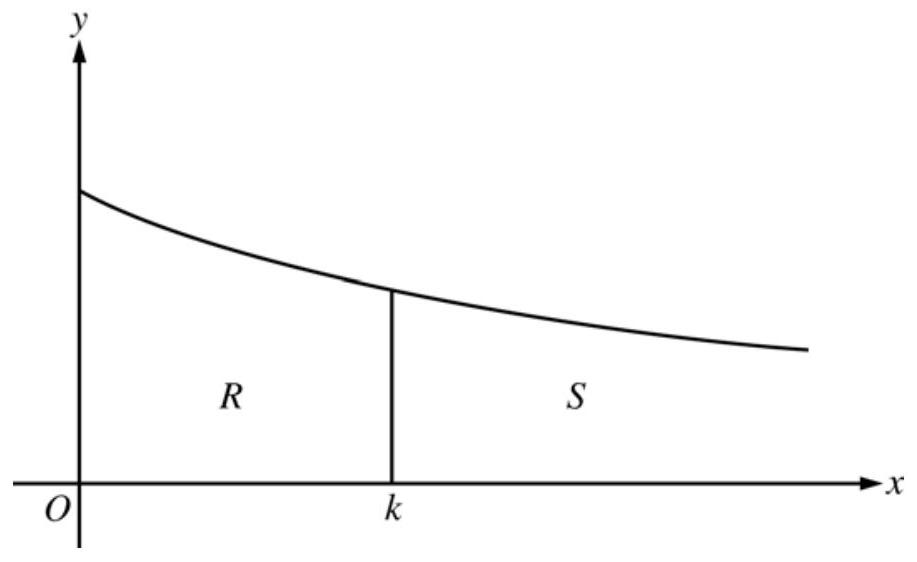
\includegraphics[width=0.6\linewidth]{figures/bc-2005-form-b_fig2.jpg}
\end{center}
Consider the graph of the function $f$ given by $f(x)=\frac{1}{x+2}$ for $x \geq 0$, as shown in the figure above. Let $R$ be the region bounded by the graph of $f$, the $x$ - and $y$-axes, and the vertical line $x=k$, where $k \geq 0$.\\
\begin{parts}
\part Find the area of $R$ in terms of $k$.
\part Find the volume of the solid generated when $R$ is revolved about the $x$-axis in terms of $k$.
\part Let $S$ be the unbounded region in the first quadrant to the right of the vertical line $x=k$ and below the graph of $f$, as shown in the figure above. Find all values of $k$ such that the volume of the solid generated when $S$ is revolved about the $x$-axis is equal to the volume of the solid found in part (b).
\end{parts}
\begin{solution}
\begin{parts}
\part Area of $R=\int_{0}^{k} \frac{1}{x+2} d x=\ln (k+2)-\ln (2)$
\part $\quad V_{R}=\pi \int_{0}^{k} \frac{1}{(x+2)^{2}} d x$

\[=-\left.\frac{\pi}{x+2}\right|_{0} ^{k}=\frac{\pi}{2}-\frac{\pi}{k+2}\]
\part $\quad V_{S}=\pi \int_{k}^{\infty} \frac{1}{(x+2)^{2}} d x$

\begin{align*}& \quad=\lim _{n \rightarrow \infty}-\left.\frac{\pi}{x+2}\right|_{k} ^{n}=\frac{\pi}{k+2} \\
& V_{S}=V_{R} \\
& \frac{\pi}{k+2}=\frac{\pi}{2}-\frac{\pi}{k+2} \\
& \frac{2}{k+2}=\frac{1}{2} \\
& k=2\end{align*}
\end{parts}
\par\medskip
\textbf{Rubric:}\par
\[\begin{aligned}
& 2:\left\{\begin{array}{c}
1: \text { integral } \\
1: \text { antidifferentiation and } \\
\text { evaluation }
\end{array}\right. \\
& 3:\left\{\begin{array}{r}
1: \text { limits } \\
1: \text { integrand } \\
1: \text { antidifferentiation and } \\
\text { evaluation }
\end{array}\right. \\
& 4:\left\{\begin{array}{l}
1: \text { improper integral } \\
1: \text { antidifferentiation and } \\
\text { evaluation } \\
1: \text { equation } \\
1: \text { answer }
\end{array}\right.
\end{aligned}\]
\end{solution}

\end{questions}

\section*{2006 AP Calculus BC}

\begin{questions}

\question
% Q1 | 2006 Calculus BC | Part A | Calculator Active
\begin{center}
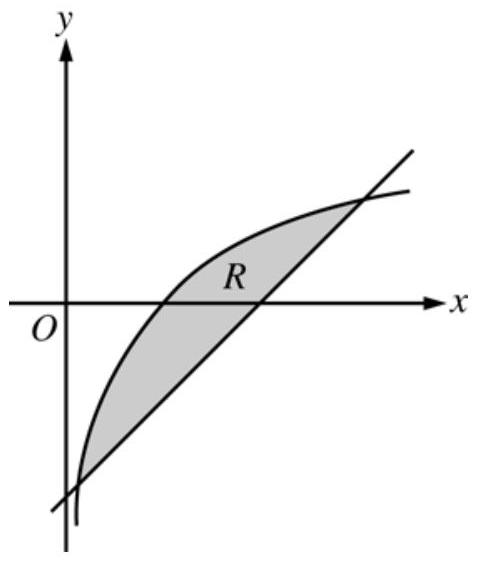
\includegraphics[width=0.6\linewidth]{figures/bc-2006_fig1.jpg}
\end{center}
Let $R$ be the shaded region bounded by the graph of $y=\ln x$ and the line $y=x-2$, as shown above.\\
\begin{parts}
\part Find the area of $R$.
\part Find the volume of the solid generated when $R$ is rotated about the horizontal line $y=-3$.
\part Write, but do not evaluate, an integral expression that can be used to find the volume of the solid generated when $R$ is rotated about the $y$-axis.
\end{parts}
\begin{solution}
\begin{parts}
\part Area of $R=\int_{S}^{T}(\ln (x)-(x-2)) d x=1.949$
\part Volume $=\pi \int_{S}^{T}\left((\ln (x)+3)^{2}-(x-2+3)^{2}\right) d x$

\[=34.198 \text { or } 34.199\]
\part $\quad$ Volume $=\pi \int_{S-2}^{T-2}\left((y+2)^{2}-\left(e^{y}\right)^{2}\right) d y$
\end{parts}
\par\medskip
\textbf{Rubric:}\par
\begin{parts}
\part $3:\left\{\begin{array}{l}
2: \text { integrand } \\
1: \text { limits and constant }
\end{array}\right.$
\end{parts}
\end{solution}

\question
% Q2 | 2006 Calculus BC | Part A | Calculator Active
\begin{center}
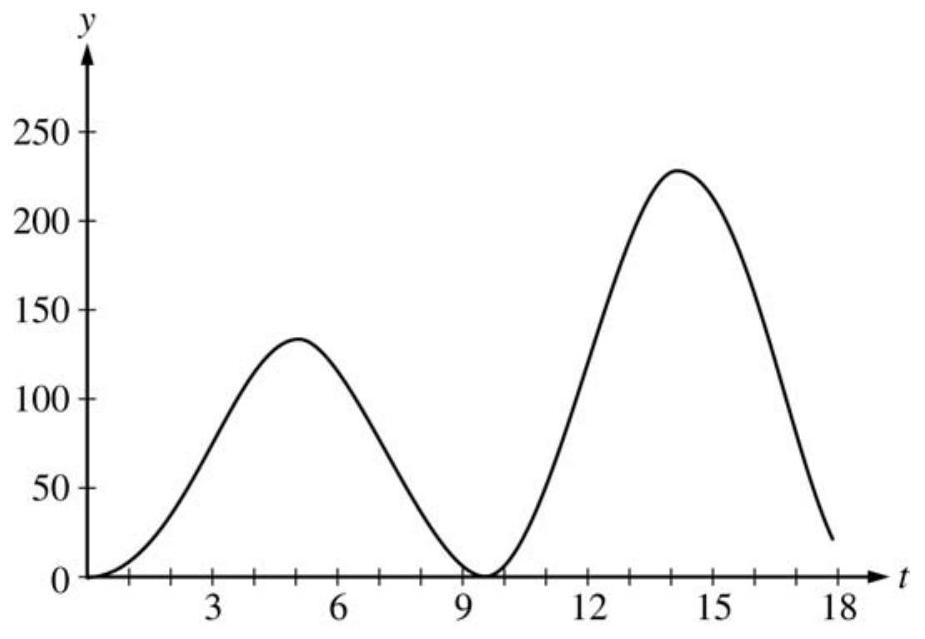
\includegraphics[width=0.6\linewidth]{figures/bc-2006_fig2.jpg}
\end{center}
At an intersection in Thomasville, Oregon, cars turn left at the rate $L(t)=60 \sqrt{t} \sin ^{2}\left(\frac{t}{3}\right)$ cars per hour over the time interval $0 \leq t \leq 18$ hours. The graph of $y=L(t)$ is shown above.\\
\begin{parts}
\part To the nearest whole number, find the total number of cars turning left at the intersection over the time interval $0 \leq t \leq 18$ hours.
\part Traffic engineers will consider turn restrictions when $L(t) \geq 150$ cars per hour. Find all values of $t$ for which $L(t) \geq 150$ and compute the average value of $L$ over this time interval. Indicate units of measure.
\part Traffic engineers will install a signal if there is any two-hour time interval during which the product of the total number of cars turning left and the total number of oncoming cars traveling straight through the intersection is greater than 200,000. In every two-hour time interval, 500 oncoming cars travel straight through the intersection. Does this intersection require a traffic signal? Explain the reasoning that leads to your conclusion.
\end{parts}
\begin{solution}
\begin{parts}
\part $\quad \int_{0}^{18} L(t) d t \approx 1658 \mathrm{cars}$
\part $L(t)=150$ when $t=12.42831,16.12166$

Let $R=12.42831$ and $S=16.12166$\\
$L(t) \geq 150$ for $t$ in the interval $[R, S]$\\
$\frac{1}{S-R} \int_{R}^{S} L(t) d t=199.426$ cars per hour
\part For the product to exceed 200,000, the number of cars turning left in a two-hour interval must be greater than 400 .\\
$\int_{13}^{15} L(t) d t=431.931>400$

The number of cars turning left will be greater than 400 on a two-hour interval if $L(t) \geq 200$ on that interval. $L(t) \geq 200$ on any two-hour subinterval of [13.25304, 15.32386].

Yes, a traffic signal is required.
\end{parts}
\par\medskip
\textbf{Rubric:}\par
\begin{parts}
\part $1: t \text {-interval when } L(t) \geq 150$
\end{parts}
\end{solution}

\question
% Q3 | 2006 Calculus BC | Part A | Calculator Active
An object moving along a curve in the $x y$-plane is at position $(x(t), y(t))$ at time $t$, where

\[\frac{d x}{d t}=\sin ^{-1}\left(1-2 e^{-t}\right) \text { and } \frac{d y}{d t}=\frac{4 t}{1+t^{3}}\]

for $t \geq 0$. At time $t=2$, the object is at the point $(6,-3)$. (Note: $\sin ^{-1} x=\arcsin x$ )\\
\begin{parts}
\part Find the acceleration vector and the speed of the object at time $t=2$.
\part The curve has a vertical tangent line at one point. At what time $t$ is the object at this point?
\part Let $m(t)$ denote the slope of the line tangent to the curve at the point $(x(t), y(t))$. Write an expression for $m(t)$ in terms of $t$ and use it to evaluate $\lim _{t \rightarrow \infty} m(t)$.
\part The graph of the curve has a horizontal asymptote $y=c$. Write, but do not evaluate, an expression involving an improper integral that represents this value $c$.
\end{parts}
\begin{solution}
\begin{parts}
\part $a(2)=\langle 0.395$ or $0.396,-0.741$ or -0.740$\rangle$

Speed $=\sqrt{x^{\prime}(2)^{2}+y^{\prime}(2)^{2}}=1.207$ or 1.208

\[2:\left\{\begin{array}{l}
1: \text { acceleration } \\
1: \text { speed }
\end{array}\right.\]
\part $\sin ^{-1}\left(1-2 e^{-t}\right)=0$\\
$1-2 e^{-t}=0$

\[2:\left\{\begin{array}{l}
1: x^{\prime}(t)=0 \\
1: \text { answer }
\end{array}\right.\]

$t=\ln 2=0.693$ and $\frac{d y}{d t} \neq 0$ when $t=\ln 2$
\part $\quad m(t)=\frac{4 t}{1+t^{3}} \cdot \frac{1}{\sin ^{-1}\left(1-2 e^{-t}\right)}$

\[\begin{aligned}
\lim _{t \rightarrow \infty} m(t) & =\lim _{t \rightarrow \infty}\left(\frac{4 t}{1+t^{3}} \cdot \frac{1}{\sin ^{-1}\left(1-2 e^{-t}\right)}\right) \\
& =0\left(\frac{1}{\sin ^{-1}(1)}\right)=0
\end{aligned}\]

\[2:\left\{\begin{array}{l}
1: m(t) \\
1: \text { limit value }
\end{array}\right.\]
\part Since $\lim _{t \rightarrow \infty} x(t)=\infty$,

\[c=\lim _{t \rightarrow \infty} y(t)=-3+\int_{2}^{\infty} \frac{4 t}{1+t^{3}} d t\]
\end{parts}
\par\medskip
\textbf{Rubric:}\par
\begin{parts}
\part $3:\left\{\begin{array}{l}
1: \text { integrand } \\
1: \text { limits } \\
1: \text { initial value consistent } \\
\quad \text { with lower limit }
\end{array}\right.$
\end{parts}
\end{solution}

\question
% Q4 | 2006 Calculus BC | Part B | Calculator Prohibited
\begin{center}
\begin{tabular}{|c|c|c|c|c|c|c|c|c|c|}
\hline
\begin{tabular}{c}
$t$ \\
(seconds) \\
\end{tabular} & 0 & 10 & 20 & 30 & 40 & 50 & 60 & 70 & 80 \\
\hline
\begin{tabular}{c}
$v(t)$ \\
(feet per second) \\
\end{tabular} & 5 & 14 & 22 & 29 & 35 & 40 & 44 & 47 & 49 \\
\hline
\end{tabular}
\end{center}
Rocket $A$ has positive velocity $v(t)$ after being launched upward from an initial height of 0 feet at time $t=0$ seconds. The velocity of the rocket is recorded for selected values of $t$ over the interval $0 \leq t \leq 80$ seconds, as shown in the table above.\\
\begin{parts}
\part Find the average acceleration of rocket $A$ over the time interval $0 \leq t \leq 80$ seconds. Indicate units of measure.
\part Using correct units, explain the meaning of $\int_{10}^{70} v(t) d t$ in terms of the rocket's flight. Use a midpoint Riemann sum with 3 subintervals of equal length to approximate $\int_{10}^{70} v(t) d t$.
\part Rocket $B$ is launched upward with an acceleration of $a(t)=\frac{3}{\sqrt{t+1}}$ feet per second per second. At time $t=0$ seconds, the initial height of the rocket is 0 feet, and the initial velocity is 2 feet per second. Which of the two rockets is traveling faster at time $t=80$ seconds? Explain your answer.
\end{parts}
\begin{solution}
\begin{parts}
\part Average acceleration of rocket $A$ is

\[\frac{v(80)-v(0)}{80-0}=\frac{49-5}{80}=\frac{11}{20} \mathrm{ft} / \mathrm{sec}^{2}\]
\part Since the velocity is positive, $\int_{10}^{70} v(t) d t$ represents the distance, in feet, traveled by rocket $A$ from $t=10$ seconds to $t=70$ seconds.

A midpoint Riemann sum is

\begin{align*}& 20[v(20)+v(40)+v(60)] \\
& =20[22+35+44]=2020 \mathrm{ft}\end{align*}
\part Let $v_{B}(t)$ be the velocity of rocket $B$ at time $t$.

\begin{align*}& v_{B}(t)=\int \frac{3}{\sqrt{t+1}} d t=6 \sqrt{t+1}+C \\
& 2=v_{B}(0)=6+C \\
& v_{B}(t)=6 \sqrt{t+1}-4 \\
& v_{B}(80)=50>49=v(80)\end{align*}

Rocket $B$ is traveling faster at time $t=80$ seconds.\\
Units of $\mathrm{ft} / \mathrm{sec}^{2}$ in (a) and ft in (b)
\end{parts}
\par\medskip
\textbf{Rubric:}\par
\begin{parts}
\part 1 : answer
\part $3:\left\{\begin{array}{l}1: \text { explanation } \\ 1: \text { uses } v(20), v(40), v(60) \\ 1: \text { value }\end{array}\right.$
\part $4:\left\{\begin{array}{l}1: 6 \sqrt{t+1} \\ 1: \text { constant of integration } \\ 1: \text { uses initial condition } \\ 1: \text { finds } v_{B}(80), \text { compares to } v(80), \\ \quad \text { and draws a conclusion }\end{array}\right.$
\part 1 : units in (a) and (b)
\end{parts}
\end{solution}

\question
% Q5 | 2006 Calculus BC | Part B | Calculator Prohibited
Consider the differential equation $\frac{d y}{d x}=5 x^{2}-\frac{6}{y-2}$ for $y \neq 2$. Let $y=f(x)$ be the particular solution to this differential equation with the initial condition $f(-1)=-4$.\\
\begin{parts}
\part Evaluate $\frac{d y}{d x}$ and $\frac{d^{2} y}{d x^{2}}$ at $(-1,-4)$.
\part Is it possible for the $x$-axis to be tangent to the graph of $f$ at some point? Explain why or why not.
\part Find the second-degree Taylor polynomial for $f$ about $x=-1$.
\part Use Euler's method, starting at $x=-1$ with two steps of equal size, to approximate $f(0)$. Show the work that leads to your answer.
\end{parts}
\begin{solution}
\begin{parts}
\part $\left.\frac{d y}{d x}\right|_{(-1,-4)}=6$\\
$\frac{d^{2} y}{d x^{2}}=10 x+6(y-2)^{-2} \frac{d y}{d x}$\\
$\left.\frac{d^{2} y}{d x^{2}}\right|_{(-1,-4)}=-10+6 \frac{1}{(-6)^{2}} 6=-9$
\part The $x$-axis will be tangent to the graph of $f$ if $\left.\frac{d y}{d x}\right|_{(k, 0)}=0$. The $x$-axis will never be tangent to the graph of $f$ because $\left.\frac{d y}{d x}\right|_{(k, 0)}=5 k^{2}+3>0$ for all $k$.
\part $P(x)=-4+6(x+1)-\frac{9}{2}(x+1)^{2}$
\part $f(-1)=-4$\\
$f\left(-\frac{1}{2}\right) \approx-4+\frac{1}{2}(6)=-1$\\
$f(0) \approx-1+\frac{1}{2}\left(\frac{5}{4}+2\right)=\frac{5}{8}$
\end{parts}
\par\medskip
\textbf{Rubric:}\par
\begin{parts}
\part $3:\left\{\begin{array}{l}
1:\left.\frac{d y}{d x}\right|_{(-1,-4)} \\
1: \frac{d^{2} y}{d x^{2}} \\
1:\left.\frac{d^{2} y}{d x^{2}}\right|_{(-1,-4)}
\end{array}\right.$
\part $2:\left\{\begin{array}{l}1: \frac{d y}{d x}=0 \text { and } y=0 \\ 1: \text { answer and explanation }\end{array}\right.$
\part $2:\left\{\begin{array}{l}1: \text { quadratic and centered at } x=-1 \\ 1: \text { coefficients }\end{array}\right.$
\part $2:\left\{\begin{array}{l}1: \text { Euler's method with } 2 \text { steps } \\ 1: \text { Euler's approximation to } f(0)\end{array}\right.$
\end{parts}
\end{solution}

\question
% Q6 | 2006 Calculus BC | Part B | Calculator Prohibited
The function $f$ is defined by the power series
\[f(x)=-\frac{x}{2}+\frac{2 x^{2}}{3}-\frac{3 x^{3}}{4}+\cdots+\frac{(-1)^{n} n x^{n}}{n+1}+\cdots\]

for all real numbers $x$ for which the series converges. The function $g$ is defined by the power series

\[g(x)=1-\frac{x}{2!}+\frac{x^{2}}{4!}-\frac{x^{3}}{6!}+\cdots+\frac{(-1)^{n} x^{n}}{(2 n)!}+\cdots\]

for all real numbers $x$ for which the series converges.\\
\begin{parts}
\part Find the interval of convergence of the power series for $f$. Justify your answer.
\part The graph of $y=f(x)-g(x)$ passes through the point $(0,-1)$. Find $y^{\prime}(0)$ and $y^{\prime \prime}(0)$. Determine whether $y$ has a relative minimum, a relative maximum, or neither at $x=0$. Give a reason for your answer.
\end{parts}
\begin{solution}
\begin{parts}
\part $\left|\frac{(-1)^{n+1}(n+1) x^{n+1}}{n+2} \cdot \frac{n+1}{(-1)^{n} n x^{n}}\right|=\frac{(n+1)^{2}}{(n+2)(n)} \cdot|x|$\\
$\lim _{n \rightarrow \infty} \frac{(n+1)^{2}}{(n+2)(n)} \cdot|x|=|x|$\\
The series converges when $-1<x<1$.\\
When $x=1$, the series is $-\frac{1}{2}+\frac{2}{3}-\frac{3}{4}+\cdots$\\
This series does not converge, because the limit of the individual terms is not zero.

When $x=-1$, the series is $\frac{1}{2}+\frac{2}{3}+\frac{3}{4}+\cdots$\\
This series does not converge, because the limit of the individual terms is not zero.

Thus, the interval of convergence is $-1<x<1$.
\part $f^{\prime}(x)=-\frac{1}{2}+\frac{4}{3} x-\frac{9}{4} x^{2}+\cdots$ and $f^{\prime}(0)=-\frac{1}{2}$.

\begin{align*}& g^{\prime}(x)=-\frac{1}{2!}+\frac{2}{4!} x-\frac{3}{6!} x^{2}+\cdots \text { and } g^{\prime}(0)=-\frac{1}{2} . \\
& y^{\prime}(0)=f^{\prime}(0)-g^{\prime}(0)=0 \\
& f^{\prime \prime}(0)=\frac{4}{3} \text { and } g^{\prime \prime}(0)=\frac{2}{4!}=\frac{1}{12} .\end{align*}
\end{parts}
\par\medskip
\textbf{Rubric:}\par
\begin{parts}
\part $4:\left\{\begin{array}{l}
1: y^{\prime}(0) \\
1: y^{\prime \prime}(0) \\
1: \text { conclusion } \\
1: \text { reasoning }
\end{array}\right.$
\part $5:\left\{\begin{array}{l}
1: \text { sets up ratio } \\
1: \text { computes limit of ratio } \\
1: \text { identifies radius of convergence } \\
1: \text { considers both endpoints } \\
1: \text { analysis/conclusion for } \\
\text { both endpoints }
\end{array}\right.$
\end{parts}
\end{solution}

\end{questions}

\section*{2006 AP Calculus BC Form B}

\begin{questions}

\question
% Q1 | 2006 Calculus BC Form B | Part A | Calculator Active
\begin{center}
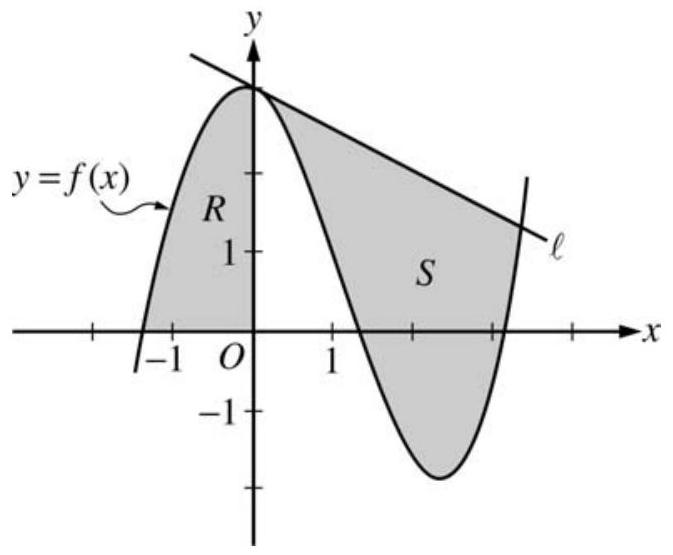
\includegraphics[width=0.6\linewidth]{figures/bc-2006-form-b_fig1.jpg}
\end{center}
Let $f$ be the function given by $f(x)=\frac{x^{3}}{4}-\frac{x^{2}}{3}-\frac{x}{2}+3 \cos x$. Let $R$ be the shaded region in the second quadrant bounded by the graph of $f$, and let $S$ be the shaded region bounded by the graph of $f$ and line $\ell$, the line tangent to the graph of $f$ at $x=0$, as shown above.\\
\begin{parts}
\part Find the area of $R$.
\part Find the volume of the solid generated when $R$ is rotated about the horizontal line $y=-2$.
\part Write, but do not evaluate, an integral expression that can be used to find the area of $S$.
\end{parts}
\begin{solution}
\begin{parts}
\part Area of $R=\int_{P}^{0} f(x) d x=2.903$
\part Volume $=\pi \int_{P}^{0}\left((f(x)+2)^{2}-4\right) d x=59.361$
\part The equation of the tangent line $\ell$ is $y=3-\frac{1}{2} x$.

The graph of $f$ and line $\ell$ intersect at $A=3.38987$.
\end{parts}
\par\medskip
\textbf{Rubric:}\par
\begin{parts}
\part $2:\left\{\begin{array}{l}
1: \text { integral } \\
1: \text { answer }
\end{array}\right.$
\part $4:\left\{\begin{array}{l}
1: \text { limits and constant } \\
2: \text { integrand } \\
1: \text { answer }
\end{array}\right.$
\part $3:\left\{\begin{array}{l}
1: \text { tangent line } \\
1: \text { integrand } \\
1: \text { limits }
\end{array}\right.$
\end{parts}
\end{solution}

\question
% Q2 | 2006 Calculus BC Form B | Part A | Calculator Active
An object moving along a curve in the $x y$-plane is at position $(x(t), y(t))$ at time $t$, where
\[\frac{d x}{d t}=\tan \left(e^{-t}\right) \text { and } \frac{d y}{d t}=\sec \left(e^{-t}\right)\]

for $t \geq 0$. At time $t=1$, the object is at position $(2,-3)$.\\
\begin{parts}
\part Write an equation for the line tangent to the curve at position $(2,-3)$.
\part Find the acceleration vector and the speed of the object at time $t=1$.
\part Find the total distance traveled by the object over the time interval $1 \leq t \leq 2$.
\part Is there a time $t \geq 0$ at which the object is on the $y$-axis? Explain why or why not.
\end{parts}
\begin{solution}
\begin{parts}
\part $\frac{d y}{d x}=\frac{\frac{d y}{d t}}{\frac{d x}{d t}}=\frac{\sec \left(e^{-t}\right)}{\tan \left(e^{-t}\right)}=\frac{1}{\sin \left(e^{-t}\right)}$

\[\begin{aligned}
& \left.\frac{d y}{d x}\right|_{(2,-3)}=\frac{1}{\sin \left(e^{-1}\right)}=2.780 \text { or } 2.781 \\
& y+3=\frac{1}{\sin \left(e^{-1}\right)}(x-2)
\end{aligned}\]
\part $x^{\prime \prime}(1)=-0.42253, y^{\prime \prime}(1)=-0.15196$

\[\begin{aligned}
& a(1)=\langle-0.423,-0.152\rangle \text { or }\langle-0.422,-0.151\rangle \\
& \text { speed }=\sqrt{\left(\sec \left(e^{-1}\right)\right)^{2}+\left(\tan \left(e^{-1}\right)\right)^{2}}=1.138 \text { or } 1.139
\end{aligned}\]
\part $\quad \int_{1}^{2} \sqrt{\left(x^{\prime}(t)\right)^{2}+\left(y^{\prime}(t)\right)^{2}} d t=1.059$
\part $\quad x(0)=x(1)-\int_{0}^{1} x^{\prime}(t) d t=2-0.775553>0$

The particle starts to the right of the $y$-axis.\\
Since $x^{\prime}(t)>0$ for all $t \geq 0$, the object is always moving to the right and thus is never on the $y$-axis.
\end{parts}
\par\medskip
\textbf{Rubric:}\par
\begin{parts}
\part 1: x(0) \text { expression }
\part $1: x^{\prime}(t)>0$
\end{parts}
\end{solution}

\question
% Q3 | 2006 Calculus BC Form B | Part A | Calculator Active
\begin{center}
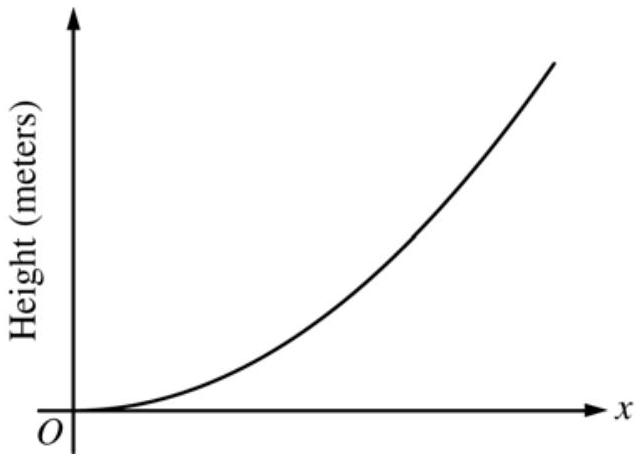
\includegraphics[width=0.6\linewidth]{figures/bc-2006-form-b_fig2.jpg}
\end{center}
The figure above is the graph of a function of $x$, which models the height of a skateboard ramp. The function meets the following requirements.\\
(i) At $x=0$, the value of the function is 0 , and the slope of the graph of the function is 0 .\\
(ii) At $x=4$, the value of the function is 1 , and the slope of the graph of the function is 1 .\\
(iii) Between $x=0$ and $x=4$, the function is increasing.\\
\begin{parts}
\part Let $f(x)=a x^{2}$, where $a$ is a nonzero constant. Show that it is not possible to find a value for $a$ so that $f$ meets requirement (ii) above.
\part Let $g(x)=c x^{3}-\frac{x^{2}}{16}$, where $c$ is a nonzero constant. Find the value of $c$ so that $g$ meets requirement (ii) above. Show the work that leads to your answer.
\part Using the function $g$ and your value of $c$ from part (b), show that $g$ does not meet requirement (iii) above.
\part Let $h(x)=\frac{x^{n}}{k}$, where $k$ is a nonzero constant and $n$ is a positive integer. Find the values of $k$ and $n$ so that $h$ meets requirement (ii) above. Show that $h$ also meets requirements (i) and (iii) above.
\end{parts}
\begin{solution}
\begin{parts}
\part $f(4)=1$ implies that $a=\frac{1}{16}$ and $f^{\prime}(4)=2 a(4)=1$ implies that $a=\frac{1}{8}$. Thus, $f$ cannot satisfy (ii).
\part $g(4)=64 c-1=1$ implies that $c=\frac{1}{32}$.

When $c=\frac{1}{32}, g^{\prime}(4)=3 c(4)^{2}-\frac{2(4)}{16}=3\left(\frac{1}{32}\right)(16)-\frac{1}{2}=1$
\part $g^{\prime}(x)=\frac{3}{32} x^{2}-\frac{x}{8}=\frac{1}{32} x(3 x-4)$\\
$g^{\prime}(x)<0$ for $0<x<\frac{4}{3}$, so $g$ does not satisfy (iii).
\part $\quad h(4)=\frac{4^{n}}{k}=1$ implies that $4^{n}=k$.\\
$h^{\prime}(4)=\frac{n 4^{n-1}}{k}=\frac{n 4^{n-1}}{4^{n}}=\frac{n}{4}=1$ gives $n=4$ and $k=4^{4}=256$.\\
$h(x)=\frac{x^{4}}{256} \Rightarrow h(0)=0$.\\
$h^{\prime}(x)=\frac{4 x^{3}}{256} \Rightarrow h^{\prime}(0)=0$ and $h^{\prime}(x)>0$ for $0<x<4$.
\end{parts}
\par\medskip
\textbf{Rubric:}\par
\begin{parts}
\part $2:\left\{\begin{array}{l}1: a=\frac{1}{16} \text { or } a=\frac{1}{8} \\ 1: \text { shows } a \text { does not work }\end{array}\right.$
\part 1 : value of $c$
\part $2:\left\{\begin{array}{l}1: g^{\prime}(x) \\ 1: \text { explanation }\end{array}\right.$
\part $4:\left\{\begin{array}{l}1: \frac{4^{n}}{k}=1 \\ 1: \frac{n 4^{n-1}}{k}=1 \\ 1: \text { values for } k \text { and } n \\ 1: \text { verifications }\end{array}\right.$
\end{parts}
\end{solution}

\question
% Q4 | 2006 Calculus BC Form B | Part B | Calculator Prohibited
\begin{center}
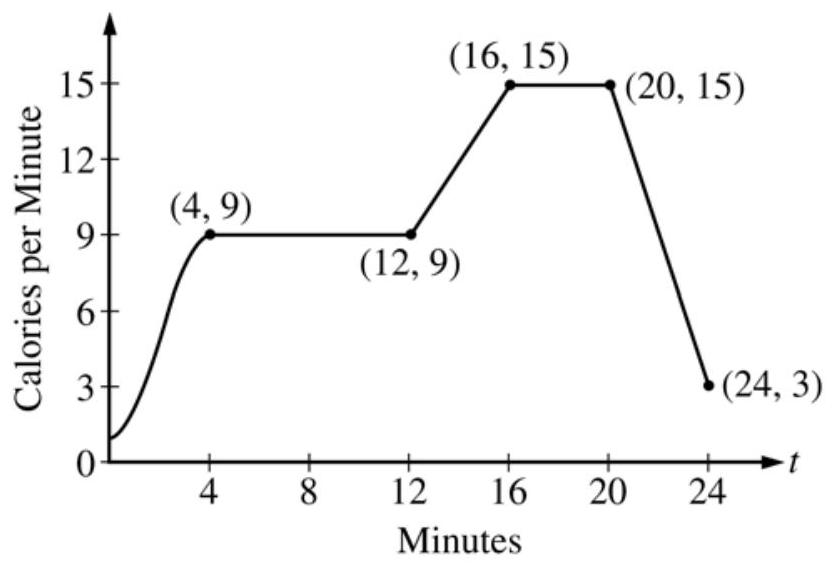
\includegraphics[width=0.6\linewidth]{figures/bc-2006-form-b_fig3.jpg}
\end{center}
The rate, in calories per minute, at which a person using an exercise machine burns calories is modeled by the function $f$. In the figure above, $f(t)=-\frac{1}{4} t^{3}+\frac{3}{2} t^{2}+1$ for $0 \leq t \leq 4$ and $f$ is piecewise linear for $4 \leq t \leq 24$.\\
\begin{parts}
\part Find $f^{\prime}(22)$. Indicate units of measure.
\part For the time interval $0 \leq t \leq 24$, at what time $t$ is $f$ increasing at its greatest rate? Show the reasoning that supports your answer.
\part Find the total number of calories burned over the time interval $6 \leq t \leq 18$ minutes.
\part The setting on the machine is now changed so that the person burns $f(t)+c$ calories per minute. For this setting, find $c$ so that an average of 15 calories per minute is burned during the time interval $6 \leq t \leq 18$.
\end{parts}
\begin{solution}
\begin{parts}
\part $\quad f^{\prime}(22)=\frac{15-3}{20-24}=-3$ calories $/ \mathrm{min} / \mathrm{min}$
\part $f$ is increasing on $[0,4]$ and on $[12,16]$.

On $(12,16), f^{\prime}(t)=\frac{15-9}{16-12}=\frac{3}{2}$ since $f$ has constant slope on this interval.\\
On $(0,4), f^{\prime}(t)=-\frac{3}{4} t^{2}+3 t$ and\\
$f^{\prime \prime}(t)=-\frac{3}{2} t+3=0$ when $t=2$. This is where $f^{\prime}$ has a maximum on $[0,4]$ since $f^{\prime \prime}>0$ on $(0,2)$ and $f^{\prime \prime}<0$ on $(2,4)$.

On [0,24], $f$ is increasing at its greatest rate when $t=2$ because $f^{\prime}(2)=3>\frac{3}{2}$.
\part $\quad \int_{6}^{18} f(t) d t=6(9)+\frac{1}{2}(4)(9+15)+2(15) =132$ calories
\part We want $\frac{1}{12} \int_{6}^{18}(f(t)+c) d t=15$.

This means $132+12 c=15(12)$. So, $c=4$.\\
OR\\
Currently, the average is $\frac{132}{12}=11$ calories $/ \mathrm{min}$.\\
Adding $c$ to $f(t)$ will shift the average by $c$.\\
So $c=4$ to get an average of 15 calories $/ \mathrm{min}$.
\end{parts}
\par\medskip
\textbf{Rubric:}\par
\begin{parts}
\part $1: f^{\prime}(22)$
\part $4:\left\{\begin{array}{l}1: f^{\prime} \text { on }(0,4) \\ 1: \text { shows } f^{\prime} \text { has a max at } t=2 \text { on }(0,4) \\ 1: \text { shows for } 12<t<16, f^{\prime}(t)<f^{\prime}(2) \\ 1: \text { answer }\end{array}\right.$
\part $2:\left\{\begin{array}{l}1: \text { method } \\ 1: \text { answer }\end{array}\right.$
\part $2:\left\{\begin{array}{l}1: \text { setup } \\ 1: \text { value of } c\end{array}\right.$
\end{parts}
\end{solution}

\question
% Q5 | 2006 Calculus BC Form B | Part B | Calculator Prohibited
Let $f$ be a function with $f(4)=1$ such that all points $(x, y)$ on the graph of $f$ satisfy the differential equation
\[\frac{d y}{d x}=2 y(3-x)\]

Let $g$ be a function with $g(4)=1$ such that all points $(x, y)$ on the graph of $g$ satisfy the logistic differential equation

\[\frac{d y}{d x}=2 y(3-y) .\]
\begin{parts}
\part Find $y=f(x)$.
\part Given that $g(4)=1$, find $\lim _{x \rightarrow \infty} g(x)$ and $\lim _{x \rightarrow \infty} g^{\prime}(x)$. (It is not necessary to solve for $g(x)$ or to show how you arrived at your answers.)
\part For what value of $y$ does the graph of $g$ have a point of inflection? Find the slope of the graph of $g$ at the point of inflection. (It is not necessary to solve for $g(x)$.)
\end{parts}
\begin{solution}
\begin{parts}
\part $\frac{d y}{d x}=2 y(3-x)$\\
$\frac{1}{y} d y=2(3-x) d x$\\
$\ln |y|=6 x-x^{2}+C$\\
$0=24-16+C$\\
$C=-8$\\
$\ln |y|=6 x-x^{2}-8$\\
$y=e^{6 x-x^{2}-8}$ for $-\infty<x<\infty$
\part $\lim _{x \rightarrow \infty} g(x)=3$\\
$\lim _{x \rightarrow \infty} g^{\prime}(x)=0$\\
$2:\left\{\begin{array}{l}1: \lim _{x \rightarrow \infty} g(x)=3 \\ 1: \lim _{x \rightarrow \infty} g^{\prime}(x)=0\end{array}\right.$
\part $\frac{d^{2} y}{d x^{2}}=(6-4 y) \frac{d y}{d x}$
\end{parts}
\par\medskip
\textbf{Rubric:}\par
\begin{parts}
\part $5:\left\{\begin{array}{l}1: \text { separates variables } \\ 1: \text { antiderivatives } \\ 1: \text { constant of integration } \\ 1: \text { uses initial condition } \\ 1: \text { solution }\end{array}\right.$
\part Note: $\max 2 / 5[1-1-0-0-0]$ if no constant of integration
\part Note: $0 / 5$ if no separation of variables
\end{parts}
\end{solution}

\question
% Q6 | 2006 Calculus BC Form B | Part B | Calculator Prohibited
The function $f$ is defined by $f(x)=\frac{1}{1+x^{3}}$. The Maclaurin series for $f$ is given by

\[1-x^{3}+x^{6}-x^{9}+\cdots+(-1)^{n} x^{3 n}+\cdots\]

which converges to $f(x)$ for $-1<x<1$.\\
\begin{parts}
\part Find the first three nonzero terms and the general term for the Maclaurin series for $f^{\prime}(x)$.
\part Use your results from part (a) to find the sum of the infinite series $-\frac{3}{2^{2}}+\frac{6}{2^{5}}-\frac{9}{2^{8}}+\cdots+(-1)^{n} \frac{3 n}{2^{3 n-1}}+\cdots$.
\part Find the first four nonzero terms and the general term for the Maclaurin series representing $\int_{0}^{x} f(t) d t$.
\part Use the first three nonzero terms of the infinite series found in part (c) to approximate $\int_{0}^{1 / 2} f(t) d t$. What are the properties of the terms of the series representing $\int_{0}^{1 / 2} f(t) d t$ that guarantee that this approximation is within $\frac{1}{10,000}$ of the exact value of the integral?
\end{parts}
\begin{solution}
\begin{parts}
\part $f^{\prime}(x)=-3 x^{2}+6 x^{5}-9 x^{8}+\cdots+3 n(-1)^{n} x^{3 n-1}+\cdots$
\part The given series is the Maclaurin series for $f^{\prime}(x)$ with $x=\frac{1}{2}$.

\[f^{\prime}(x)=-\left(1+x^{3}\right)^{-2}\left(3 x^{2}\right)\]

Thus, the sum of the series is $f^{\prime}\left(\frac{1}{2}\right)=-\frac{3\left(\frac{1}{4}\right)}{\left(1+\frac{1}{8}\right)^{2}}=-\frac{16}{27}$.
\part $\quad \int_{0}^{x} \frac{1}{1+t^{3}} d t=x-\frac{x^{4}}{4}+\frac{x^{7}}{7}-\frac{x^{10}}{10}+\cdots+\frac{(-1)^{n} x^{3 n+1}}{3 n+1}+\cdots$
\part $\quad \int_{0}^{1 / 2} \frac{1}{1+t^{3}} d t \approx \frac{1}{2}-\frac{\left(\frac{1}{2}\right)^{4}}{4}+\frac{\left(\frac{1}{2}\right)^{7}}{7}$.

The series in part (c) with $x=\frac{1}{2}$ has terms that alternate, decrease in absolute value, and have limit 0 . Hence the error is bounded by the absolute value of the next term.

\[\left|\int_{0}^{1 / 2} \frac{1}{1+t^{3}} d t-\left(\frac{1}{2}-\frac{\left(\frac{1}{2}\right)^{4}}{4}+\frac{\left(\frac{1}{2}\right)^{7}}{7}\right)\right|<\frac{\left(\frac{1}{2}\right)^{10}}{10}=\frac{1}{10240}<0.0001\]
\end{parts}
\par\medskip
\textbf{Rubric:}\par
\begin{parts}
\part $1: f^{\prime}(x)$
\part $1: f^{\prime}\left(\frac{1}{2}\right)$
\end{parts}
\end{solution}

\end{questions}

\section*{2007 AP Calculus BC}

\begin{questions}

\question
% Q1 | 2007 Calculus BC | Part A | Calculator Active
Let $R$ be the region in the first and second quadrants bounded above by the graph of $y=\frac{20}{1+x^{2}}$ and below by the horizontal line $y=2$.\\
\begin{parts}
\part Find the area of $R$.
\part Find the volume of the solid generated when $R$ is rotated about the $x$-axis.
\part The region $R$ is the base of a solid. For this solid, the cross sections perpendicular to the $x$-axis are semicircles. Find the volume of this solid.
\end{parts}
\begin{solution}
\begin{parts}
\part Area $=\int_{-3}^{3}\left(\frac{20}{1+x^{2}}-2\right) d x=37.961$ or 37.962
\part Volume $=\pi \int_{-3}^{3}\left(\left(\frac{20}{1+x^{2}}\right)^{2}-2^{2}\right) d x=1871.190$
\part Volume $=\frac{\pi}{2} \int_{-3}^{3}\left(\frac{1}{2}\left(\frac{20}{1+x^{2}}-2\right)\right)^{2} d x$

\[=\frac{\pi}{8} \int_{-3}^{3}\left(\frac{20}{1+x^{2}}-2\right)^{2} d x=174.268\]
\end{parts}
\par\medskip
\textbf{Rubric:}\par
\begin{parts}
\part 1 : correct limits in an integral in (a), (b), or (c)
\part $2:\left\{\begin{array}{l}1: \text { integrand } \\ 1: \text { answer }\end{array}\right.$
\part $3:\left\{\begin{array}{l}2: \text { integrand } \\ 1: \text { answer }\end{array}\right.$
\part $3:\left\{\begin{array}{l}2: \text { integrand } \\ 1: \text { answer }\end{array}\right.$
\end{parts}
\end{solution}

\question
% Q2 | 2007 Calculus BC | Part A | Calculator Active
\begin{center}
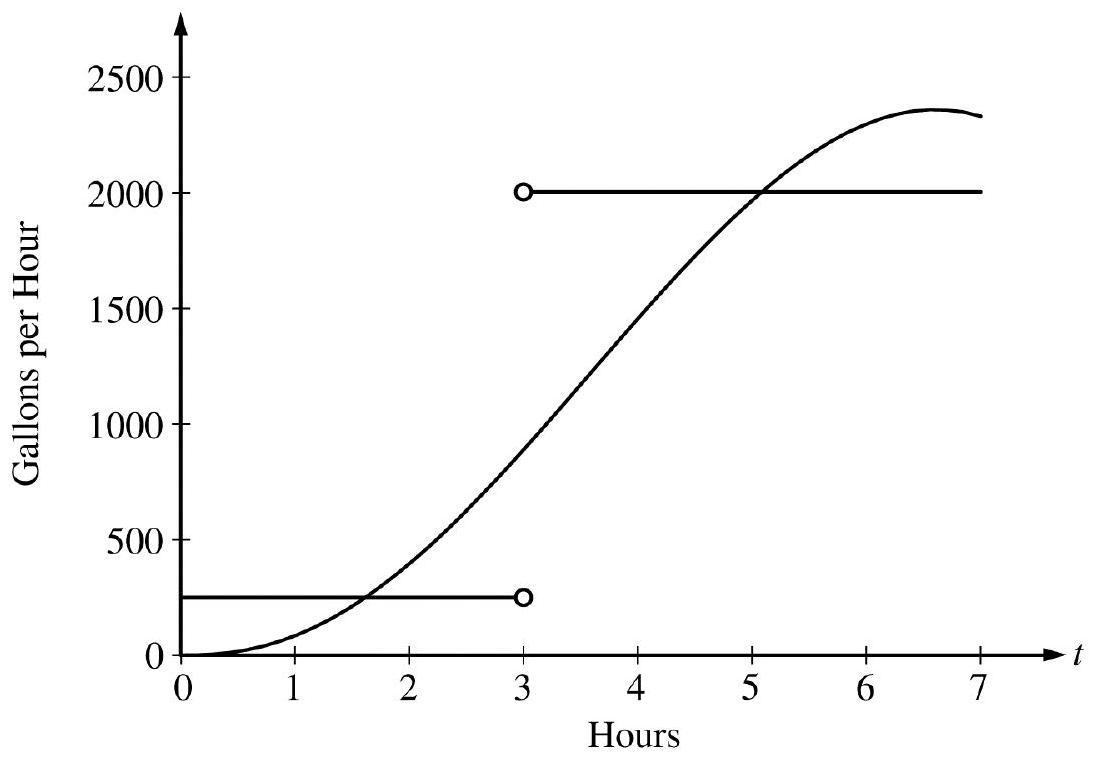
\includegraphics[width=0.6\linewidth]{figures/bc-2007_fig1.jpg}
\end{center}
The amount of water in a storage tank, in gallons, is modeled by a continuous function on the time interval $0 \leq t \leq 7$, where $t$ is measured in hours. In this model, rates are given as follows:\\
(i) The rate at which water enters the tank is $f(t)=100 t^{2} \sin (\sqrt{t})$ gallons per hour for $0 \leq t \leq 7$.\\
(ii) The rate at which water leaves the tank is
\[g(t)=\left\{\begin{array}{r}
250 \text { for } 0 \leq t<3 \\
2000 \text { for } 3<t \leq 7
\end{array}\right. \text { gallons per hour. }\]

The graphs of $f$ and $g$, which intersect at $t=1.617$ and $t=5.076$, are shown in the figure above. At time $t=0$, the amount of water in the tank is 5000 gallons.\\
\begin{parts}
\part How many gallons of water enter the tank during the time interval $0 \leq t \leq 7$ ? Round your answer to the nearest gallon.
\part For $0 \leq t \leq 7$, find the time intervals during which the amount of water in the tank is decreasing. Give a reason for each answer.
\part For $0 \leq t \leq 7$, at what time $t$ is the amount of water in the tank greatest? To the nearest gallon, compute the amount of water at this time. Justify your answer.
\end{parts}
\begin{solution}
\begin{parts}
\part $\quad \int_{0}^{7} f(t) d t \approx 8264$ gallons
\part The amount of water in the tank is decreasing on the intervals $0 \leq t \leq 1.617$ and $3 \leq t \leq 5.076$ because $f(t)<g(t)$ for $0 \leq t<1.617$ and $3<t<5.076$.
\part Since $f(t)-g(t)$ changes sign from positive to negative only at $t=3$, the candidates for the absolute maximum are at $t=0,3$, and 7 .

\begin{center}
\begin{tabular}{|c|l|}
\hline
$t$ (hours) & gallons of water \\
\hline
0 & 5000 \\
\hline
3 & $5000+\int_{0}^{3} f(t) d t-250(3)=5126.591$ \\
\hline
7 & $5126.591+\int_{3}^{7} f(t) d t-2000(4)=4513.807$ \\
\hline
\end{tabular}
\end{center}

The amount of water in the tank is greatest at 3 hours. At that time, the amount of water in the tank, rounded to the nearest gallon, is 5127 gallons.
\end{parts}
\par\medskip
\textbf{Rubric:}\par
\begin{parts}
\part $2:\left\{\begin{array}{l}
1: \text { integral } \\
1: \text { answer }
\end{array}\right.$
\part $2:\left\{\begin{array}{l}
1: \text { intervals } \\
1: \text { reason }
\end{array}\right.$
\part $5:\left\{\begin{array}{l}
1: \text { identifies } t=3 \text { as a candidate } \\
1: \text { integrand } \\
1: \text { amount of water at } t=3 \\
1: \text { amount of water at } t=7 \\
1: \text { conclusion }
\end{array}\right.$
\end{parts}
\end{solution}

\question
% Q3 | 2007 Calculus BC | Part A | Calculator Active
\begin{center}
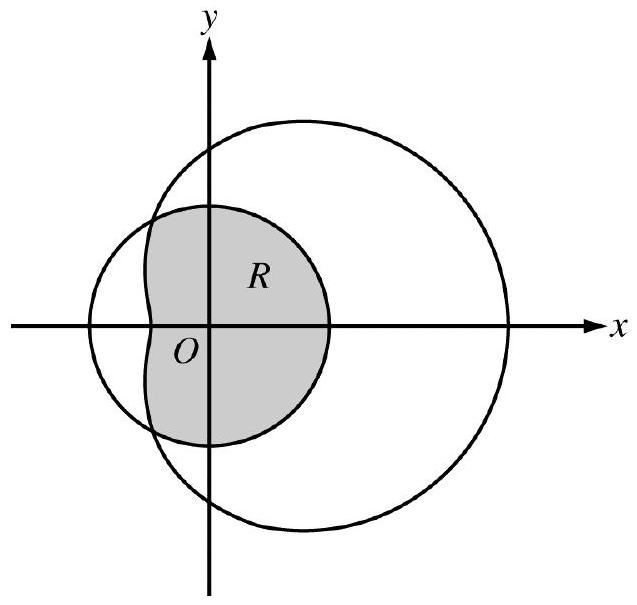
\includegraphics[width=0.6\linewidth]{figures/bc-2007_fig2.jpg}
\end{center}
The graphs of the polar curves $r=2$ and $r=3+2 \cos \theta$ are shown in the figure above. The curves intersect when $\theta=\frac{2 \pi}{3}$ and $\theta=\frac{4 \pi}{3}$.\\
\begin{parts}
\part Let $R$ be the region that is inside the graph of $r=2$ and also inside the graph of $r=3+2 \cos \theta$, as shaded in the figure above. Find the area of $R$.
\part A particle moving with nonzero velocity along the polar curve given by $r=3+2 \cos \theta$ has position $(x(t), y(t))$ at time $t$, with $\theta=0$ when $t=0$. This particle moves along the curve so that $\frac{d r}{d t}=\frac{d r}{d \theta}$. Find the value of $\frac{d r}{d t}$ at $\theta=\frac{\pi}{3}$ and interpret your answer in terms of the motion of the particle.
\part For the particle described in part (b), $\frac{d y}{d t}=\frac{d y}{d \theta}$. Find the value of $\frac{d y}{d t}$ at $\theta=\frac{\pi}{3}$ and interpret your answer in terms of the motion of the particle.
\end{parts}
\begin{solution}
\begin{parts}
\part Area $=\frac{2}{3} \pi(2)^{2}+\frac{1}{2} \int_{2 \pi / 3}^{4 \pi / 3}(3+2 \cos \theta)^{2} d \theta$

\[\text { = } 10.370\]

\[4:\left\{\begin{aligned}
1 & : \text { area of circular sector } \\
2 & : \text { integral for section of limaçon } \\
1 & : \text { integrand } \\
1 & : \text { limits and constant } \\
1 & : \text { answer }
\end{aligned}\right.\]
\part $y=r \sin \theta=(3+2 \cos \theta) \sin \theta$

\[\left.\frac{d y}{d t}\right|_{\theta=\pi / 3}=\left.\frac{d y}{d \theta}\right|_{\theta=\pi / 3}=0.5\]
\part $\left.\frac{d r}{d t}\right|_{\theta=\pi / 3}=\left.\frac{d r}{d \theta}\right|_{\theta=\pi / 3}=-1.732$

\begin{align*}& \text { The particle is moving closer to the origin, since } \frac{d r}{d t}<0 \\
& \text { and } r>0 \text { when } \theta=\frac{\pi}{3} \text {. }\end{align*}
\end{parts}
\par\medskip
\textbf{Rubric:}\par
\begin{parts}
\part $3:\left\{\begin{array}{l}
1: \text { expression for } y \text { in terms of } \theta \\
1:\left.\frac{d y}{d t}\right|_{\theta=\pi / 3} \\
1: \text { interpretation }
\end{array}\right.$
\end{parts}
\end{solution}

\question
% Q4 | 2007 Calculus BC | Part B | Calculator Prohibited
Let $f$ be the function defined for $x>0$, with $f(e)=2$ and $f^{\prime}$, the first derivative of $f$, given by $f^{\prime}(x)=x^{2} \ln x$.\\
\begin{parts}
\part Write an equation for the line tangent to the graph of $f$ at the point $(e, 2)$.
\part Is the graph of $f$ concave up or concave down on the interval $1<x<3$ ? Give a reason for your answer.
\part Use antidifferentiation to find $f(x)$.
\end{parts}
\begin{solution}
\begin{parts}
\part $f^{\prime}(e)=e^{2}$

An equation for the line tangent to the graph of $f$ at the point $(e, 2)$ is $y-2=e^{2}(x-e)$.
\part $f^{\prime \prime}(x)=x+2 x \ln x$.

For $1<x<3, x>0$ and $\ln x>0$, so $f^{\prime \prime}(x)>0$. Thus, the graph of $f$ is concave up on $(1,3)$.
\part Since $f(x)=\int\left(x^{2} \ln x\right) d x$, we consider integration by parts.

\[\begin{array}{ll}
u=\ln x & d v=x^{2} d x \\
d u=\frac{1}{x} d x & v=\int\left(x^{2}\right) d x=\frac{1}{3} x^{3}
\end{array}\]

Therefore,

\[\begin{aligned}
f(x) & =\int\left(x^{2} \ln x\right) d x \\
& =\frac{1}{3} x^{3} \ln x-\int\left(\frac{1}{3} x^{3} \cdot \frac{1}{x}\right) d x \\
& =\frac{1}{3} x^{3} \ln x-\frac{1}{9} x^{3}+C
\end{aligned}\]

Since $f(e)=2,2=\frac{e^{3}}{3}-\frac{e^{3}}{9}+C$ and $C=2-\frac{2}{9} e^{3}$.\\
Thus, $f(x)=\frac{x^{3}}{3} \ln x-\frac{1}{9} x^{3}+2-\frac{2}{9} e^{3}$.
\end{parts}
\par\medskip
\textbf{Rubric:}\par
\begin{parts}
\part $2:\left\{\begin{array}{l}
1: f^{\prime}(e) \\
1: \text { equation of tangent line }
\end{array}\right.$
\part $3:\left\{\begin{array}{l}
2: f^{\prime \prime}(x) \\
1: \text { answer with reason }
\end{array}\right.$
\part $4:\left\{\begin{array}{l}
2: \text { antiderivative } \\
1: \text { uses } f(e)=2 \\
1: \text { answer }
\end{array}\right.$
\end{parts}
\end{solution}

\question
% Q5 | 2007 Calculus BC | Part B | Calculator Prohibited
\begin{center}
\begin{tabular}{|c|c|c|c|c|c|c|}
\hline
\begin{tabular}{c}
$t$ \\
(minutes) \\
\end{tabular} & 0 & 2 & 5 & 7 & 11 & 12 \\
\hline
\begin{tabular}{c}
$r^{\prime}(t)$ \\
(feet per minute) \\
\end{tabular} & 5.7 & 4.0 & 2.0 & 1.2 & 0.6 & 0.5 \\
\hline
\end{tabular}
\end{center}
The volume of a spherical hot air balloon expands as the air inside the balloon is heated. The radius of the balloon, in feet, is modeled by a twice-differentiable function $r$ of time $t$, where $t$ is measured in minutes. For $0<t<12$, the graph of $r$ is concave down. The table above gives selected values of the rate of change, $r^{\prime}(t)$, of the radius of the balloon over the time interval $0 \leq t \leq 12$. The radius of the balloon is 30 feet when $t=5$.\\
(Note: The volume of a sphere of radius $r$ is given by $V=\frac{4}{3} \pi r^{3}$.)\\
\begin{parts}
\part Estimate the radius of the balloon when $t=5.4$ using the tangent line approximation at $t=5$. Is your estimate greater than or less than the true value? Give a reason for your answer.
\part Find the rate of change of the volume of the balloon with respect to time when $t=5$. Indicate units of measure.
\part Use a right Riemann sum with the five subintervals indicated by the data in the table to approximate $\int_{0}^{12} r^{\prime}(t) d t$. Using correct units, explain the meaning of $\int_{0}^{12} r^{\prime}(t) d t$ in terms of the radius of the balloon.
\part Is your approximation in part (c) greater than or less than $\int_{0}^{12} r^{\prime}(t) d t$ ? Give a reason for your answer.
\end{parts}
\begin{solution}
\begin{parts}
\part $r(5.4) \approx r(5)+r^{\prime}(5) \Delta t=30+2(0.4)=30.8 \mathrm{ft}$ Since the graph of $r$ is concave down on the interval $5<t<5.4$, this estimate is greater than $r$ (5.4).
\part $\frac{d V}{d t}=3\left(\frac{4}{3}\right) \pi r^{2} \frac{d r}{d t} \left.\frac{d V}{d t}\right|_{t=5}=4 \pi(30)^{2} 2=7200 \pi \mathrm{ft}^{3} / \mathrm{min}$
\part $\int_{0}^{12} r^{\prime}(t) d t \approx 2(4.0)+3(2.0)+2(1.2)+4(0.6)+1(0.5) =19.3 \mathrm{ft} \int_{0}^{12} r^{\prime}(t) d t$ is the change in the radius, in feet, from $t=0$ to $t=12$ minutes.
\part Since $r$ is concave down, $r^{\prime}$ is decreasing on $0<t<12$. Therefore, this approximation, 19.3 ft , is less than $\int_{0}^{12} r^{\prime}(t) d t$.

Units of $\mathrm{ft}^{3} / \mathrm{min}$ in part (b) and ft in part (c)
\end{parts}
\par\medskip
\textbf{Rubric:}\par
\begin{parts}
\part $2:\left\{\begin{array}{l}1: \text { estimate } \\ 1: \text { conclusion with reason }\end{array}\right.$
\part $3:\left\{\begin{array}{l}2: \frac{d V}{d t} \\ 1: \text { answer }\end{array}\right.$
\part $2:\left\{\begin{array}{l}1: \text { approximation } \\ 1: \text { explanation }\end{array}\right.$
\part 1 : conclusion with reason
\part 1 : units in (b) and (c)
\end{parts}
\end{solution}

\question
% Q6 | 2007 Calculus BC | Part B | Calculator Prohibited
Let $f$ be the function given by $f(x)=e^{-x^{2}}$.\\
\begin{parts}
\part Write the first four nonzero terms and the general term of the Taylor series for $f$ about $x=0$.
\part Use your answer to part (a) to find $\lim _{x \rightarrow 0} \frac{1-x^{2}-f(x)}{x^{4}}$.
\part Write the first four nonzero terms of the Taylor series for $\int_{0}^{x} e^{-t^{2}} d t$ about $x=0$. Use the first two terms of your answer to estimate $\int_{0}^{1 / 2} e^{-t^{2}} d t$.
\part Explain why the estimate found in part (c) differs from the actual value of $\int_{0}^{1 / 2} e^{-t^{2}} d t$ by less than $\frac{1}{200}$.
\end{parts}
\begin{solution}
\begin{parts}
\part $e^{-x^{2}}=1+\frac{\left(-x^{2}\right)}{1!}+\frac{\left(-x^{2}\right)^{2}}{2!}+\frac{\left(-x^{2}\right)^{3}}{3!}+\cdots+\frac{\left(-x^{2}\right)^{n}}{n!}+\cdots$

\[=1-x^{2}+\frac{x^{4}}{2}-\frac{x^{6}}{6}+\cdots+\frac{(-1)^{n} x^{2 n}}{n!}+\cdots\]
\part $\frac{1-x^{2}-f(x)}{x^{4}}=-\frac{1}{2}+\frac{x^{2}}{6}+\sum_{n=4}^{\infty} \frac{(-1)^{n+1} x^{2 n-4}}{n!}$

Thus, $\lim _{x \rightarrow 0}\left(\frac{1-x^{2}-f(x)}{x^{4}}\right)=-\frac{1}{2}$.
\part $\int_{0}^{x} e^{-t^{2}} d t=\int_{0}^{x}\left(1-t^{2}+\frac{t^{4}}{2}-\frac{t^{6}}{6}+\cdots+\frac{(-1)^{n} t^{2 n}}{n!}+\cdots\right) d t$

\[=x-\frac{x^{3}}{3}+\frac{x^{5}}{10}-\frac{x^{7}}{42}+\cdots\]

Using the first two terms of this series, we estimate that\\
$\int_{0}^{1 / 2} e^{-t^{2}} d t \approx \frac{1}{2}-\left(\frac{1}{3}\right)\left(\frac{1}{8}\right)=\frac{11}{24}$.
\part $\left|\int_{0}^{1 / 2} e^{-t^{2}} d t-\frac{11}{24}\right|<\left(\frac{1}{2}\right)^{5} \cdot \frac{1}{10}=\frac{1}{320}<\frac{1}{200}$, since $\int_{0}^{1 / 2} e^{-t^{2}} d t=\sum_{n=0}^{\infty} \frac{(-1)^{n}\left(\frac{1}{2}\right)^{2 n+1}}{n!(2 n+1)}$, which is an alternating series with individual terms that decrease in absolute value to 0 .
\end{parts}
\par\medskip
\textbf{Rubric:}\par
\begin{parts}
\part $3:\left\{\begin{array}{l}1: \text { two of } 1,-x^{2}, \frac{x^{4}}{2},-\frac{x^{6}}{6} \\ 1: \text { remaining terms } \\ 1: \text { general term }\end{array}\right.$
\part 1 : answer
\part $3:\left\{\begin{array}{l}1: \text { two terms } \\ 1: \text { remaining terms } \\ 1: \text { estimate }\end{array}\right.$
\part $2:\left\{\begin{array}{l}1: \text { uses the third term as } \\ \quad \text { the error bound } \\ 1: \text { explanation }\end{array}\right.$
\end{parts}
\end{solution}

\end{questions}

\section*{2007 AP Calculus BC Form B}

\begin{questions}

\question
% Q1 | 2007 Calculus BC Form B | Part A | Calculator Active
\begin{center}
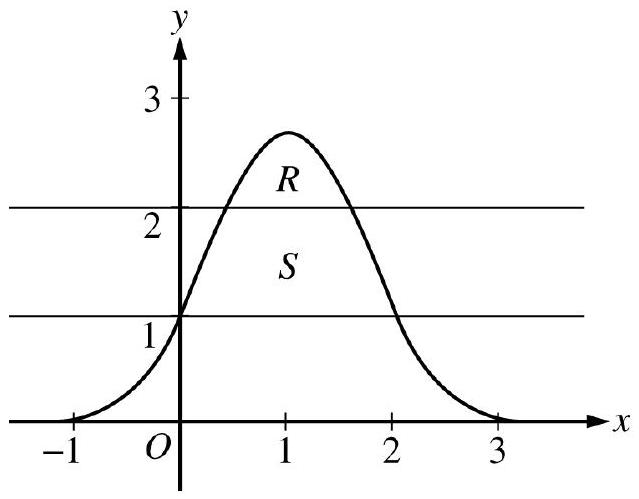
\includegraphics[width=0.6\linewidth]{figures/bc-2007-form-b_fig1.jpg}
\end{center}
Let $R$ be the region bounded by the graph of $y=e^{2 x-x^{2}}$ and the horizontal line $y=2$, and let $S$ be the region bounded by the graph of $y=e^{2 x-x^{2}}$ and the horizontal lines $y=1$ and $y=2$, as shown above.\\
\begin{parts}
\part Find the area of $R$.
\part Find the area of $S$.
\part Write, but do not evaluate, an integral expression that gives the volume of the solid generated when $R$ is rotated about the horizontal line $y=1$.
\end{parts}
\begin{solution}
\begin{parts}
\part Area of $R=\int_{P}^{Q}\left(e^{2 x-x^{2}}-2\right) d x=0.514$\\
$3:\left\{\begin{array}{l}1: \text { integrand } \\ 1: \text { limits } \\ 1: \text { answer }\end{array}\right.$
\part $e^{2 x-x^{2}}=1$ when $x=0,2$

Area of $S=\int_{0}^{2}\left(e^{2 x-x^{2}}-1\right) d x-$ Area of $R$

\[=2.06016-\text { Area of } R=1.546\]

OR

\[\begin{aligned}
& \int_{0}^{P}\left(e^{2 x-x^{2}}-1\right) d x+(Q-P) \cdot 1+\int_{Q}^{2}\left(e^{2 x-x^{2}}-1\right) d x \\
& =0.219064+1.107886+0.219064=1.546
\end{aligned}\]

$3:\left\{\begin{array}{l}1: \text { integrand } \\ 1: \text { limits } \\ 1: \text { answer }\end{array}\right.$
\part Volume $=\pi \int_{P}^{Q}\left(\left(e^{2 x-x^{2}}-1\right)^{2}-(2-1)^{2}\right) d x$
\end{parts}
\par\medskip
\textbf{Rubric:}\par
\begin{parts}
\part $3:\left\{\begin{array}{l}2: \text { integrand } \\ 1: \text { constant and limits }\end{array}\right.$
\end{parts}
\end{solution}

\question
% Q2 | 2007 Calculus BC Form B | Part A | Calculator Active
An object moving along a curve in the $x y$-plane is at position $(x(t), y(t))$ at time $t$ with
\[\frac{d x}{d t}=\arctan \left(\frac{t}{1+t}\right) \text { and } \frac{d y}{d t}=\ln \left(t^{2}+1\right)\]

for $t \geq 0$. At time $t=0$, the object is at position $(-3,-4)$. (Note: $\tan ^{-1} x=\arctan x$ )\\
\begin{parts}
\part Find the speed of the object at time $t=4$.
\part Find the total distance traveled by the object over the time interval $0 \leq t \leq 4$.
\part Find $x(4)$.
\part For $t>0$, there is a point on the curve where the line tangent to the curve has slope 2 . At what time $t$ is the object at this point? Find the acceleration vector at this point.
\end{parts}
\begin{solution}
\begin{parts}
\part Speed $=\sqrt{x^{\prime}(4)^{2}+y^{\prime}(4)^{2}}=2.912$
\part Distance $=\int_{0}^{4} \sqrt{\left(\frac{d x}{d t}\right)^{2}+\left(\frac{d y}{d t}\right)^{2}} d t=6.423$
\part $x(4)=x(0)+\int_{0}^{4} x^{\prime}(t) d t$

\[=-3+2.10794=-0.892\]
\part The slope is 2, so $\frac{\frac{d y}{d t}}{\frac{d x}{d t}}=2$, or $\ln \left(t^{2}+1\right)=2 \arctan \left(\frac{t}{1+t}\right)$.

Since $t>0, t=1.35766$. At this time, the acceleration is $\left.\left\langle x^{\prime \prime}(t), y^{\prime \prime}(t)\right\rangle\right|_{t=1.35766}=\langle 0.135,0.955\rangle$.
\end{parts}
\par\medskip
\textbf{Rubric:}\par
\begin{parts}
\part 1 : speed at $t=4$
\part $2:\left\{\begin{array}{l}1: \text { integral } \\ 1: \text { answer }\end{array}\right.$
\part $3:\left\{\begin{array}{l}2:\left\{\begin{array}{l}1: \text { integrand } \\ 1: \text { uses } x(0)=-3\end{array}\right. \\ 1: \text { answer }\end{array}\right.$
\part $3:\left\{\begin{array}{l}1: \frac{\frac{d y}{d t}}{\frac{d x}{d t}}=2 \\ 1: t \text {-value } \\ 1: \text { values for } x^{\prime \prime} \text { and } y^{\prime \prime}\end{array}\right.$
\end{parts}
\end{solution}

\question
% Q3 | 2007 Calculus BC Form B | Part A | Calculator Active
The wind chill is the temperature, in degrees Fahrenheit ( ${ }^{\circ} \mathrm{F}$ ), a human feels based on the air temperature, in degrees Fahrenheit, and the wind velocity $v$, in miles per hour (mph). If the air temperature is $32^{\circ} \mathrm{F}$, then the wind chill is given by $W(v)=55.6-22.1 v^{0.16}$ and is valid for $5 \leq v \leq 60$.\\
\begin{parts}
\part Find $W^{\prime}(20)$. Using correct units, explain the meaning of $W^{\prime}(20)$ in terms of the wind chill.
\part Find the average rate of change of $W$ over the interval $5 \leq v \leq 60$. Find the value of $v$ at which the instantaneous rate of change of $W$ is equal to the average rate of change of $W$ over the interval $5 \leq v \leq 60$.
\part Over the time interval $0 \leq t \leq 4$ hours, the air temperature is a constant $32^{\circ} \mathrm{F}$. At time $t=0$, the wind velocity is $v=20 \mathrm{mph}$. If the wind velocity increases at a constant rate of 5 mph per hour, what is the rate of change of the wind chill with respect to time at $t=3$ hours? Indicate units of measure.
\end{parts}
\begin{solution}
\begin{parts}
\part $W^{\prime}(20)=-22.1 \cdot 0.16 \cdot 20^{-0.84}=-0.285$ or -0.286

When $v=20 \mathrm{mph}$, the wind chill is decreasing at $0.286^{\circ} \mathrm{F} / \mathrm{mph}$.
\part The average rate of change of $W$ over the interval

\begin{align*}& 5 \leq v \leq 60 \text { is } \frac{W(60)-W(5)}{60-5}=-0.253 \text { or }-0.254 . \\
& W^{\prime}(v)=\frac{W(60)-W(5)}{60-5} \text { when } v=23.011 .\end{align*}
\part $\left.\quad \frac{d W}{d t}\right|_{t=3}=\left.\left(\frac{d W}{d v} \cdot \frac{d v}{d t}\right)\right|_{t=3}=W^{\prime}(35) \cdot 5=-0.892{ }^{\circ} \mathrm{F} / \mathrm{hr}$

OR

\begin{align*}& W=55.6-22.1(20+5 t)^{0.16} \\
& \left.\frac{d W}{d t}\right|_{t=3}=-0.892^{\circ} \mathrm{F} / \mathrm{hr}\end{align*}

Units of ${ }^{\circ} \mathrm{F} / \mathrm{mph}$ in (a) and ${ }^{\circ} \mathrm{F} / \mathrm{hr}$ in (c)
\end{parts}
\par\medskip
\textbf{Rubric:}\par
\begin{parts}
\part $2:\left\{\begin{array}{l}
1: \text { value } \\
1: \text { explanation }
\end{array}\right.$
\part $3:\left\{\begin{array}{l}
1: \text { average rate of change } \\
1: W^{\prime}(v)=\text { average rate of change } \\
1: \text { value of } v
\end{array}\right.$
\part $3:\left\{\begin{array}{l}
1: \frac{d v}{d t}=5 \\
1: \text { uses } v(3)=35, \\
\quad \text { or } \\
\quad \text { uses } v(t)=20+5 t \\
1: \text { answer }
\end{array}\right.$
\part 1 : units in (a) and (c)
\end{parts}
\end{solution}

\question
% Q4 | 2007 Calculus BC Form B | Part B | Calculator Prohibited
\begin{center}
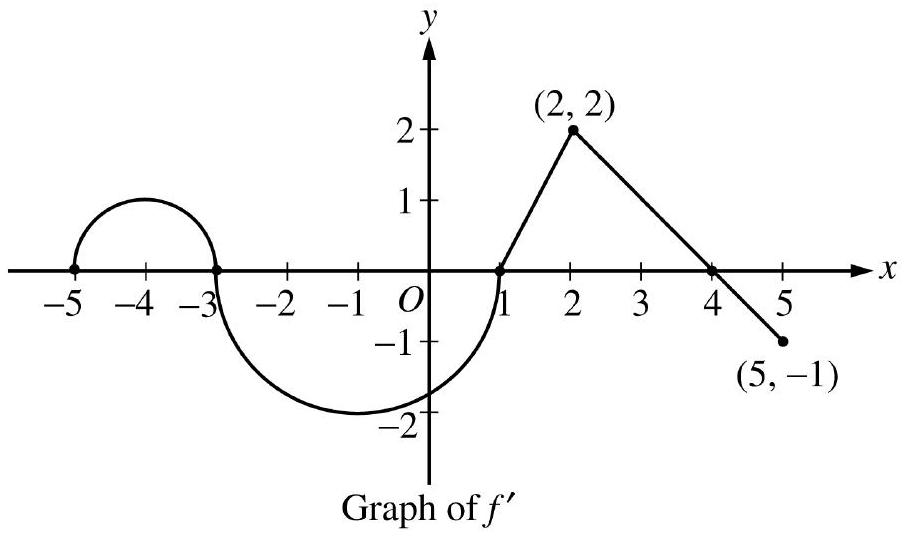
\includegraphics[width=0.6\linewidth]{figures/bc-2007-form-b_fig2.jpg}
\end{center}
Let $f$ be a function defined on the closed interval $-5 \leq x \leq 5$ with $f(1)=3$. The graph of $f^{\prime}$, the derivative of $f$, consists of two semicircles and two line segments, as shown above.\\
\begin{parts}
\part For $-5<x<5$, find all values $x$ at which $f$ has a relative maximum. Justify your answer.
\part For $-5<x<5$, find all values $x$ at which the graph of $f$ has a point of inflection. Justify your answer.
\part Find all intervals on which the graph of $f$ is concave up and also has positive slope. Explain your reasoning.
\part Find the absolute minimum value of $f(x)$ over the closed interval $-5 \leq x \leq 5$. Explain your reasoning.
\end{parts}
\begin{solution}
\begin{parts}
\part $\quad f^{\prime}(x)=0$ at $x=-3,1,4$\\
$f^{\prime}$ changes from positive to negative at -3 and 4 .\\
Thus, $f$ has a relative maximum at $x=-3$ and at $x=4$.
\part $f^{\prime}$ changes from increasing to decreasing, or vice versa, at $x=-4,-1$, and 2 . Thus, the graph of $f$ has points of inflection when $x=-4,-1$, and 2 .
\part The graph of $f$ is concave up with positive slope where $f^{\prime}$ is increasing and positive: $-5<x<-4$ and $1<x<2$.
\part Candidates for the absolute minimum are where $f^{\prime}$ changes from negative to positive (at $x=1$ ) and at the endpoints ( $x=-5,5$ ).

\begin{align*}& f(-5)=3+\int_{1}^{-5} f^{\prime}(x) d x=3-\frac{\pi}{2}+2 \pi>3 \\
& f(1)=3 \\
& f(5)=3+\int_{1}^{5} f^{\prime}(x) d x=3+\frac{3 \cdot 2}{2}-\frac{1}{2}>3\end{align*}

The absolute minimum value of $f$ on $[-5,5]$ is $f(1)=3$.
\end{parts}
\par\medskip
\textbf{Rubric:}\par
\begin{parts}
\part $2:\left\{\begin{array}{l}
1: x \text {-values } \\
1: \text { justification }
\end{array}\right.$
\part $2:\left\{\begin{array}{l}1: x \text {-values } \\ 1: \text { justification }\end{array}\right.$
\part $2:\left\{\begin{array}{l}
1: \text { intervals } \\
1: \text { explanation }
\end{array}\right.$
\part $3:\left\{\begin{array}{l}
1: \text { identifies } x=1 \text { as a candidate } \\
1: \text { considers endpoints } \\
1: \text { value and explanation }
\end{array}\right.$
\end{parts}
\end{solution}

\question
% Q5 | 2007 Calculus BC Form B | Part B | Calculator Prohibited
Consider the differential equation $\frac{d y}{d x}=3 x+2 y+1$.\\
\begin{parts}
\part Find $\frac{d^{2} y}{d x^{2}}$ in terms of $x$ and $y$.
\part Find the values of the constants $m, b$, and $r$ for which $y=m x+b+e^{r x}$ is a solution to the differential equation.
\part Let $y=f(x)$ be a particular solution to the differential equation with the initial condition $f(0)=-2$. Use Euler's method, starting at $x=0$ with a step size of $\frac{1}{2}$, to approximate $f(1)$. Show the work that leads to your answer.
\part Let $y=g(x)$ be another solution to the differential equation with the initial condition $g(0)=k$, where $k$ is a constant. Euler's method, starting at $x=0$ with a step size of 1 , gives the approximation $g(1) \approx 0$. Find the value of $k$.
\end{parts}
\begin{solution}
\begin{parts}
\part $\frac{d^{2} y}{d x^{2}}=3+2 \frac{d y}{d x}=3+2(3 x+2 y+1)=6 x+4 y+5$
\part If $y=m x+b+e^{r x}$ is a solution, then

\[m+r e^{r x}=3 x+2\left(m x+b+e^{r x}\right)+1\]

If $r \neq 0: m=2 b+1, r=2,0=3+2 m$, so $m=-\frac{3}{2}, r=2$, and $b=-\frac{5}{4}$.

If $r=0: m=2 b+3, r=0,0=3+2 m$, so $m=-\frac{3}{2}, r=0, b=-\frac{9}{4}$.
\part $f\left(\frac{1}{2}\right) \approx f(0)+f^{\prime}(0) \cdot \frac{1}{2}=-2+(-3) \cdot \frac{1}{2}=-\frac{7}{2}$

\[f^{\prime}\left(\frac{1}{2}\right) \approx 3\left(\frac{1}{2}\right)+2\left(-\frac{7}{2}\right)+1=-\frac{9}{2}\]

$f(1) \approx f\left(\frac{1}{2}\right)+f^{\prime}\left(\frac{1}{2}\right) \cdot \frac{1}{2}=-\frac{7}{2}+\left(-\frac{9}{2}\right) \cdot \frac{1}{2}=-\frac{23}{4}$
\part $g^{\prime}(0)=3 \cdot 0+2 \cdot k+1=2 k+1$\\
$g(1) \approx g(0)+g^{\prime}(0) \cdot 1=k+(2 k+1)=3 k+1=0$\\
$k=-\frac{1}{3}$
\end{parts}
\par\medskip
\textbf{Rubric:}\par
\begin{parts}
\part $2:\left\{\begin{array}{l}1: 3+2 \frac{d y}{d x} \\ 1: \text { answer }\end{array}\right.$
\part $3:\left\{\begin{array}{l}1: \frac{d y}{d x}=m+r e^{r x} \\ 1: \text { value for } r \\ 1: \text { values for } m \text { and } b\end{array}\right.$
\part $2:\left\{\begin{array}{l}
1: \text { Euler's method with } 2 \text { steps } \\
1: \text { Euler's approximation for } f(1)
\end{array}\right.$
\part $2:\left\{\begin{array}{l}1: g(0)+g^{\prime}(0) \cdot 1 \\ 1: \text { value of } k\end{array}\right.$
\end{parts}
\end{solution}

\question
% Q6 | 2007 Calculus BC Form B | Part B | Calculator Prohibited
Let $f$ be the function given by $f(x)=6 e^{-x / 3}$ for all $x$.\\
\begin{parts}
\part Find the first four nonzero terms and the general term for the Taylor series for $f$ about $x=0$.
\part Let $g$ be the function given by $g(x)=\int_{0}^{x} f(t) d t$. Find the first four nonzero terms and the general term for the Taylor series for $g$ about $x=0$.
\part The function $h$ satisfies $h(x)=k f^{\prime}(a x)$ for all $x$, where $a$ and $k$ are constants. The Taylor series for $h$ about $x=0$ is given by
\[h(x)=1+x+\frac{x^{2}}{2!}+\frac{x^{3}}{3!}+\cdots+\frac{x^{n}}{n!}+\cdots\]

Find the values of $a$ and $k$.
\end{parts}
\begin{solution}
\begin{parts}
\part $f(x)=6\left[1-\frac{x}{3}+\frac{x^{2}}{2!3^{2}}-\frac{x^{3}}{3!3^{3}}+\cdots+\frac{(-1)^{n} x^{n}}{n!3^{n}}+\cdots\right]$

\[=6-2 x+\frac{x^{2}}{3}-\frac{x^{3}}{27}+\cdots+\frac{6(-1)^{n} x^{n}}{n!3^{n}}+\cdots\]
\part $\quad g(0)=0$ and $g^{\prime}(x)=f(x)$, so

\[\begin{aligned}
g(x) & =6\left[x-\frac{x^{2}}{6}+\frac{x^{3}}{3!3^{2}}-\frac{x^{4}}{4!3^{3}}+\cdots+\frac{(-1)^{n} x^{n+1}}{(n+1)!3^{n}}+\cdots\right] \\
& =6 x-x^{2}+\frac{x^{3}}{9}-\frac{x^{4}}{4(27)}+\cdots+\frac{6(-1)^{n} x^{n+1}}{(n+1)!3^{n}}+\cdots
\end{aligned}\]
\part $f^{\prime}(x)=-2 e^{-x / 3}$, so $h(x)=-2 k e^{-a x / 3}$

\begin{align*}& h(x)=1+x+\frac{x^{2}}{2!}+\frac{x^{3}}{3!}+\cdots+\frac{x^{n}}{n!}+\cdots=e^{x} \\
& -2 k e^{-a x / 3}=e^{x} \\
& \frac{-a}{3}=1 \text { and }-2 k=1 \\
& a=-3 \text { and } k=-\frac{1}{2}\end{align*}

OR

\begin{align*}& f^{\prime}(x)=-2+\frac{2}{3} x+\cdots, \text { so } \\
& h(x)=k f^{\prime}(a x)=-2 k+\frac{2}{3} a k x+\cdots \\
& h(x)=1+x+\cdots \\
& -2 k=1 \text { and } \frac{2}{3} a k=1 \\
& k=-\frac{1}{2} \text { and } a=-3\end{align*}

\[\left.\begin{array}{rl}
3: & \left\{\begin{array}{l}
1: \text { two of } 6,-2 x, \frac{x^{2}}{3},-\frac{x^{3}}{27} \\
1: \text { remaining terms } \\
1: \text { general term }
\end{array}\right. \\
& \langle-1\rangle \text { missing factor of } 6 \\
3:\{ & \left\{\begin{array}{l}
1: \text { two terms } \\
1: \text { remaining terms } \\
1: \text { general term }
\end{array}\right. \\
& \langle-1\rangle \text { missing factor of } 6
\end{array}\right]=\left\{\begin{array}{c}
1: \text { computes } k f^{\prime}(a x) \\
1: \text { recognizes } h(x)=e^{x}, \\
\text { or } \\
\text { equates } 2 \text { series for } h(x) \\
1: \text { values for } a \text { and } k
\end{array}{ }_{3:}\right.\]
\end{parts}
\end{solution}

\end{questions}

\section*{2008 AP Calculus BC}

\begin{questions}

\question
% Q1 | 2008 Calculus BC | Part A | Calculator Active
\begin{center}
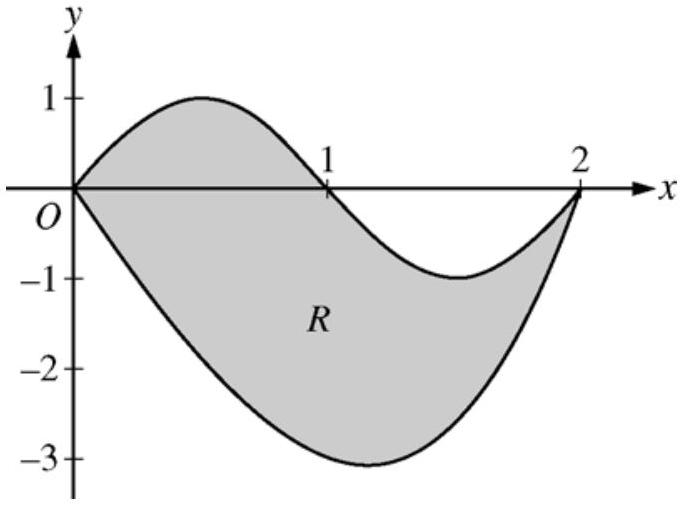
\includegraphics[width=0.6\linewidth]{figures/bc-2008_fig1.jpg}
\end{center}
Let $R$ be the region bounded by the graphs of $y=\sin (\pi x)$ and $y=x^{3}-4 x$, as shown in the figure above.\\
\begin{parts}
\part Find the area of $R$.
\part The horizontal line $y=-2$ splits the region $R$ into two parts. Write, but do not evaluate, an integral expression for the area of the part of $R$ that is below this horizontal line.
\part The region $R$ is the base of a solid. For this solid, each cross section perpendicular to the $x$-axis is a square. Find the volume of this solid.
\part The region $R$ models the surface of a small pond. At all points in $R$ at a distance $x$ from the $y$-axis, the depth of the water is given by $h(x)=3-x$. Find the volume of water in the pond.
\end{parts}
\begin{solution}
\begin{parts}
\part $\sin (\pi x)=x^{3}-4 x$ at $x=0$ and $x=2$

\[\text { Area }=\int_{0}^{2}\left(\sin (\pi x)-\left(x^{3}-4 x\right)\right) d x=4\]

\[3:\left\{\begin{array}{l}
1: \text { limits } \\
1: \text { integrand } \\
1: \text { answer }
\end{array}\right.\]
\part $x^{3}-4 x=-2$ at $r=0.5391889$ and $s=1.6751309$

The area of the stated region is $\int_{r}^{s}\left(-2-\left(x^{3}-4 x\right)\right) d x$

\[2:\left\{\begin{array}{l}
1: \text { limits } \\
1: \text { integrand }
\end{array}\right.\]
\part Volume $=\int_{0}^{2}\left(\sin (\pi x)-\left(x^{3}-4 x\right)\right)^{2} d x=9.978$

\[2:\left\{\begin{array}{l}
1: \text { integrand } \\
1: \text { answer }
\end{array}\right.\]
\part Volume $=\int_{0}^{2}(3-x)\left(\sin (\pi x)-\left(x^{3}-4 x\right)\right) d x=8.369$ or 8.370
\end{parts}
\par\medskip
\textbf{Rubric:}\par
\begin{parts}
\part $2:\left\{\begin{array}{l}1: \text { integrand } \\ 1: \text { answer }\end{array}\right.$
\end{parts}
\end{solution}

\question
% Q2 | 2008 Calculus BC | Part A | Calculator Active
\begin{center}
\begin{tabular}{|c||c|c|c|c|c|c|c|}
\hline
$t$ (hours) & 0 & 1 & 3 & 4 & 7 & 8 & 9 \\
\hline
$L(t)$ (people) & 120 & 156 & 176 & 126 & 150 & 80 & 0 \\
\hline
\end{tabular}
\end{center}
Concert tickets went on sale at noon $(t=0)$ and were sold out within 9 hours. The number of people waiting in line to purchase tickets at time $t$ is modeled by a twice-differentiable function $L$ for $0 \leq t \leq 9$. Values of $L(t)$ at various times $t$ are shown in the table above.\\
\begin{parts}
\part Use the data in the table to estimate the rate at which the number of people waiting in line was changing at 5:30 P.M. $(t=5.5)$. Show the computations that lead to your answer. Indicate units of measure.
\part Use a trapezoidal sum with three subintervals to estimate the average number of people waiting in line during the first 4 hours that tickets were on sale.
\part For $0 \leq t \leq 9$, what is the fewest number of times at which $L^{\prime}(t)$ must equal 0 ? Give a reason for your answer.
\part The rate at which tickets were sold for $0 \leq t \leq 9$ is modeled by $r(t)=550 t e^{-t / 2}$ tickets per hour. Based on the model, how many tickets were sold by 3 P.M. ( $t=3$ ), to the nearest whole number?
\end{parts}
\begin{solution}
\begin{parts}
\part $L^{\prime}(5.5) \approx \frac{L(7)-L(4)}{7-4}=\frac{150-126}{3}=8$ people per hour
\part The average number of people waiting in line during the first 4 hours is approximately

\[\begin{aligned}
& \frac{1}{4}\left(\frac{L(0)+L(1)}{2}(1-0)+\frac{L(1)+L(3)}{2}(3-1)+\frac{L(3)+L(4)}{2}(4-3)\right) \\
& =155.25 \text { people }
\end{aligned}\]
\part $L$ is differentiable on $[0,9]$ so the Mean Value Theorem implies $L^{\prime}(t)>0$ for some $t$ in ( 1,3 ) and some $t$ in ( 4,7 ). Similarly, $L^{\prime}(t)<0$ for some $t$ in (3,4) and some $t$ in (7,8). Then, since $L^{\prime}$ is continuous on [0,9], the Intermediate Value Theorem implies that $L^{\prime}(t)=0$ for at least three values of $t$ in $[0,9]$.

The continuity of $L$ on $[1,4]$ implies that $L$ attains a maximum value there. Since $L(3)>L(1)$ and $L(3)>L(4)$, this maximum occurs on (1,4). Similarly, $L$ attains a minimum on (3,7) and a maximum on $(4,8) . L$ is differentiable, so $L^{\prime}(t)=0$ at each relative extreme point on ( 0,9 ). Therefore $L^{\prime}(t)=0$ for at least three values of $t$ in $[0,9]$.\\[0pt]
[Note: There is a function $L$ that satisfies the given conditions with $L^{\prime}(t)=0$ for exactly three values of $t$.]
\part $\int_{0}^{3} r(t) d t=972.784$

There were approximately 973 tickets sold by 3 P.M.

\begin{verbatim}
$2:\left\{\begin{array}{l}1: \text { estimate } \\ 1: \text { units }\end{array}\right.$
$2:\left\{\begin{array}{l}1: \text { trapezoidal sum } \\ 1: \text { answer }\end{array}\right.$
$3:\left\{\begin{array}{l}1: \text { considers change in } \\ \quad \text { sign of } L^{\prime} \\ 1: \text { analysis } \\ 1: \text { conclusion }\end{array}\right.$
\end{verbatim}

\begin{center}
\end{center}
\end{parts}
\end{solution}

\question
% Q3 | 2008 Calculus BC | Part A | Calculator Active
\begin{center}
\begin{tabular}{|c||c|c|c|c|c|}
\hline
$x$ & $h(x)$ & $h^{\prime}(x)$ & $h^{\prime \prime}(x)$ & $h^{\prime \prime \prime}(x)$ & $h^{(4)}(x)$ \\
\hline
1 & 11 & 30 & 42 & 99 & 18 \\
\hline
2 & 80 & 128 & $\frac{488}{3}$ & $\frac{448}{3}$ & $\frac{584}{9}$ \\
\hline
3 & 317 & $\frac{753}{2}$ & $\frac{1383}{4}$ & $\frac{3483}{16}$ & $\frac{1125}{16}$ \\
\hline
\end{tabular}
\end{center}
Let $h$ be a function having derivatives of all orders for $x>0$. Selected values of $h$ and its first four derivatives are indicated in the table above. The function $h$ and these four derivatives are increasing on the interval $1 \leq x \leq 3$.\\
\begin{parts}
\part Write the first-degree Taylor polynomial for $h$ about $x=2$ and use it to approximate $h(1.9)$. Is this approximation greater than or less than $h(1.9)$ ? Explain your reasoning.
\part Write the third-degree Taylor polynomial for $h$ about $x=2$ and use it to approximate $h(1.9)$.
\part Use the Lagrange error bound to show that the third-degree Taylor polynomial for $h$ about $x=2$ approximates $h(1.9)$ with error less than $3 \times 10^{-4}$.
\end{parts}
\begin{solution}
\begin{parts}
\part $P_{1}(x)=80+128(x-2)$, so $h(1.9) \approx P_{1}(1.9)=67.2$\\
$P_{1}(1.9)<h(1.9)$ since $h^{\prime}$ is increasing on the interval $1 \leq x \leq 3$.
\part $P_{3}(x)=80+128(x-2)+\frac{488}{6}(x-2)^{2}+\frac{448}{18}(x-2)^{3} h(1.9) \approx P_{3}(1.9)=67.988$
\part The fourth derivative of $h$ is increasing on the interval $1 \leq x \leq 3$, so $\max _{1.9 \leq x \leq 2}\left|h^{(4)}(x)\right|=\frac{584}{9}$.\\
Therefore, $\left|h(1.9)-P_{3}(1.9)\right| \leq \frac{584}{9} \frac{|1.9-2|^{4}}{4!}$

\begin{align*}& =2.7037 \times 10^{-4} \\
& <3 \times 10^{-4}\end{align*}
\end{parts}
\par\medskip
\textbf{Rubric:}\par
\begin{parts}
\part $4:\left\{\begin{array}{l}
2: P_{1}(x) \\
1: P_{1}(1.9) \\
1: P_{1}(1.9)<h(1.9) \text { with reason }
\end{array}\right.$
\part $3:\left\{\begin{array}{l}
2: P_{3}(x) \\
1: P_{3}(1.9)
\end{array}\right.$
\part $2:\left\{\begin{array}{l}
1: \text { form of Lagrange error estimate } \\
1: \text { reasoning }
\end{array}\right.$
\end{parts}
\end{solution}

\question
% Q4 | 2008 Calculus BC | Part B | Calculator Prohibited
\begin{center}
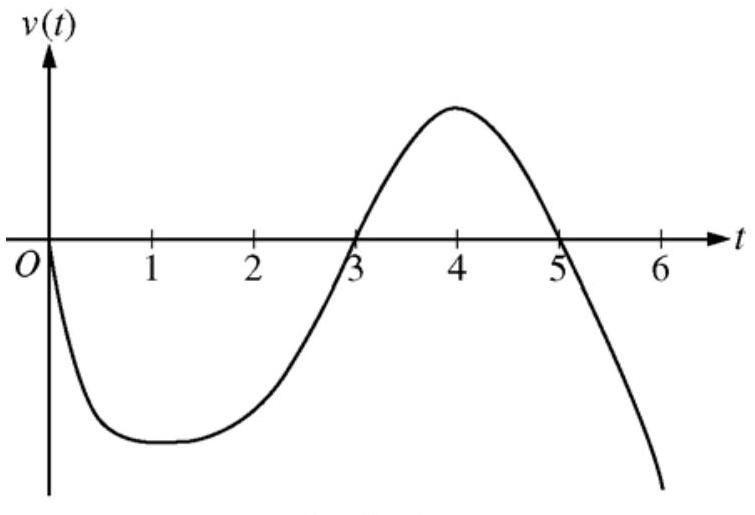
\includegraphics[width=0.6\linewidth]{figures/bc-2008_fig2.jpg}
\end{center}

Graph of $v$\\
A particle moves along the $x$-axis so that its velocity at time $t$, for $0 \leq t \leq 6$, is given by a differentiable function $v$ whose graph is shown above. The velocity is 0 at $t=0, t=3$, and $t=5$, and the graph has horizontal tangents at $t=1$ and $t=4$. The areas of the regions bounded by the $t$-axis and the graph of $v$ on the intervals $[0,3],[3,5]$, and $[5,6]$ are 8,3 , and 2 , respectively. At time $t=0$, the particle is at $x=-2$.\\
\begin{parts}
\part For $0 \leq t \leq 6$, find both the time and the position of the particle when the particle is farthest to the left. Justify your answer.
\part For how many values of $t$, where $0 \leq t \leq 6$, is the particle at $x=-8$ ? Explain your reasoning.
\part On the interval $2<t<3$, is the speed of the particle increasing or decreasing? Give a reason for your answer.
\part During what time intervals, if any, is the acceleration of the particle negative? Justify your answer.
\end{parts}
\begin{solution}
\begin{parts}
\part Since $v(t)<0$ for $0<t<3$ and $5<t<6$, and $v(t)>0$ for $3<t<5$, we consider $t=3$ and $t=6$.

\begin{align*}& x(3)=-2+\int_{0}^{3} v(t) d t=-2-8=-10 \\
& x(6)=-2+\int_{0}^{6} v(t) d t=-2-8+3-2=-9\end{align*}

Therefore, the particle is farthest left at time $t=3$ when its position is $x(3)=-10$.
\part The particle moves continuously and monotonically from $x(0)=-2$ to $x(3)=-10$. Similarly, the particle moves continuously and monotonically from $x(3)=-10$ to $x(5)=-7$ and also from $x(5)=-7$ to $x(6)=-9$.

By the Intermediate Value Theorem, there are three values of $t$ for which the particle is at $x(t)=-8$.
\part The speed is decreasing on the interval $2<t<3$ since on this interval $v<0$ and $v$ is increasing.
\part The acceleration is negative on the intervals $0<t<1$ and $4<t<6$ since velocity is decreasing on these intervals.
\end{parts}
\par\medskip
\textbf{Rubric:}\par
\begin{parts}
\part $3:\left\{\begin{array}{l}1: \text { identifies } t=3 \text { as a candidate } \\ 1: \text { considers } \int_{0}^{6} v(t) d t \\ 1: \text { conclusion }\end{array}\right.$
\part $3:\left\{\begin{aligned}
1: & \text { positions at } t=3, t=5, \\
& \text { and } t=6 \\
1: & \text { description of motion } \\
1: & \text { conclusion }
\end{aligned}\right.$
\part 1 : answer with reason
\part $2:\left\{\begin{array}{l}1: \text { answer } \\ 1: \text { justification }\end{array}\right.$
\end{parts}
\end{solution}

\question
% Q5 | 2008 Calculus BC | Part B | Calculator Prohibited
The derivative of a function $f$ is given by $f^{\prime}(x)=(x-3) e^{x}$ for $x>0$, and $f(1)=7$.\\
\begin{parts}
\part The function $f$ has a critical point at $x=3$. At this point, does $f$ have a relative minimum, a relative maximum, or neither? Justify your answer.
\part On what intervals, if any, is the graph of $f$ both decreasing and concave up? Explain your reasoning.
\part Find the value of $f(3)$.
\end{parts}
\begin{solution}
\begin{parts}
\part $f^{\prime}(x)<0$ for $0<x<3$ and $f^{\prime}(x)>0$ for $x>3$

Therefore, $f$ has a relative minimum at $x=3$.
\part $f^{\prime \prime}(x)=e^{x}+(x-3) e^{x}=(x-2) e^{x}$\\
$f^{\prime \prime}(x)>0$ for $x>2$\\
$f^{\prime}(x)<0$ for $0<x<3$

Therefore, the graph of $f$ is both decreasing and concave up on the interval $2<x<3$.
\part $f(3)=f(1)+\int_{1}^{3} f^{\prime}(x) d x=7+\int_{1}^{3}(x-3) e^{x} d x$

\[\begin{array}{cc}
u=x-3 & d v=e^{x} d x \\
d u=d x & v=e^{x}
\end{array}\]

\[\begin{aligned}
f(3) & =7+\left.(x-3) e^{x}\right|_{1} ^{3}-\int_{1}^{3} e^{x} d x \\
& =7+\left.\left((x-3) e^{x}-e^{x}\right)\right|_{1} ^{3} \\
& =7+3 e-e^{3}
\end{aligned}\]
\end{parts}
\par\medskip
\textbf{Rubric:}\par
\begin{parts}
\part $2:\left\{\begin{array}{l}
1: \text { minimum at } x=3 \\
1: \text { justification }
\end{array}\right.$
\part $3:\left\{\begin{array}{l}2: f^{\prime \prime}(x) \\ 1: \text { answer with reason }\end{array}\right.$
\part 4: $\left\{\begin{array}{l}1: \text { uses initial condition } \\ 2: \text { integration by parts } \\ 1: \text { answer }\end{array}\right.$
\end{parts}
\end{solution}

\question
% Q6 | 2008 Calculus BC | Part B | Calculator Prohibited
Consider the logistic differential equation $\frac{d y}{d t}=\frac{y}{8}(6-y)$. Let $y=f(t)$ be the particular solution to the differential equation with $f(0)=8$.\\
\begin{parts}
\part A slope field for this differential equation is given below. Sketch possible solution curves through the points $(3,2)$ and $(0,8)$.\\
\begin{center}
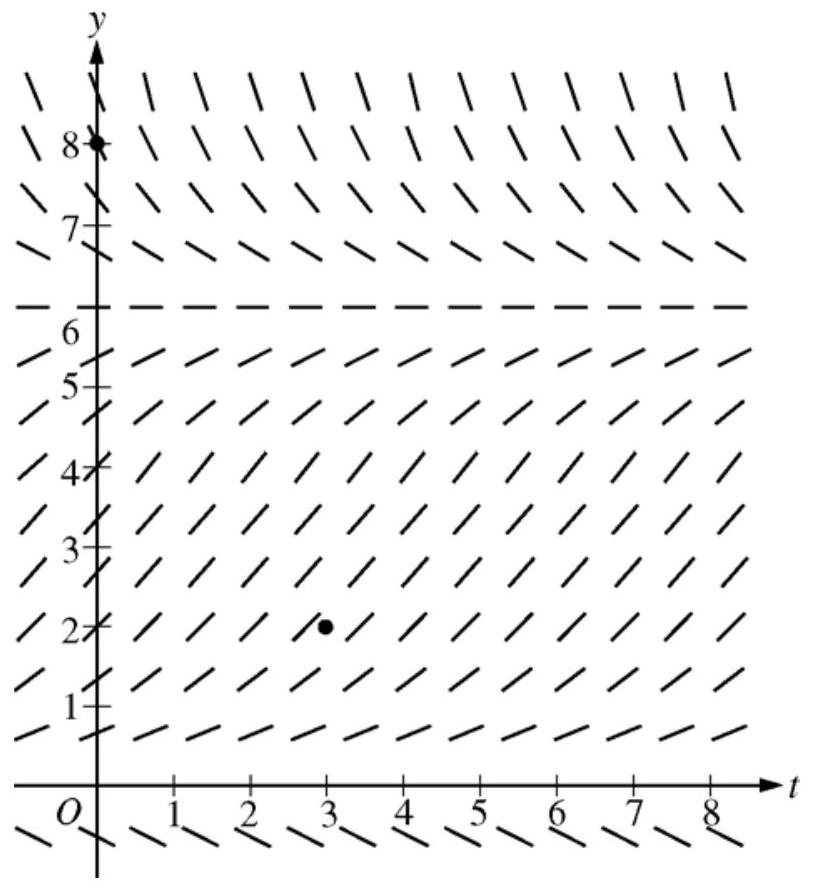
\includegraphics[width=0.6\linewidth]{figures/bc-2008_fig3.jpg}
\end{center}
\part Use Euler's method, starting at $t=0$ with two steps of equal size, to approximate $f(1)$.
\part Write the second-degree Taylor polynomial for $f$ about $t=0$, and use it to approximate $f(1)$.
\part What is the range of $f$ for $t \geq 0$ ?
\end{parts}
\begin{solution}
(a)\\
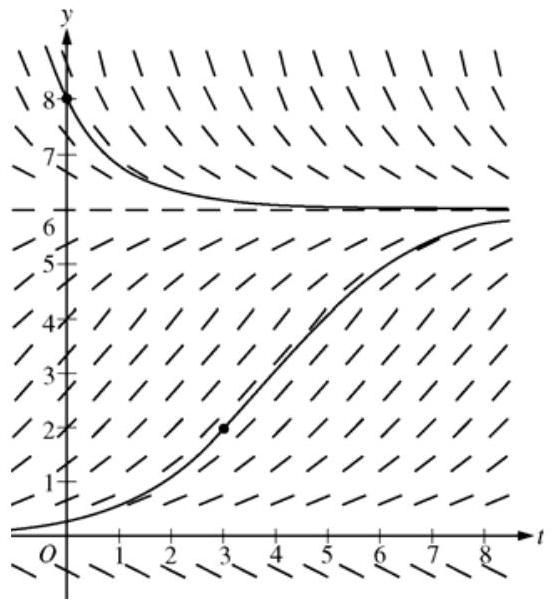
\includegraphics[width=0.6\linewidth]{figures/sg-bc-2008_fig4.jpg}\\
\begin{parts}
\part $f\left(\frac{1}{2}\right) \approx 8+(-2)\left(\frac{1}{2}\right)=7$\\
$f(1) \approx 7+\left(-\frac{7}{8}\right)\left(\frac{1}{2}\right)=\frac{105}{16}$
\part $\frac{d^{2} y}{d t^{2}}=\frac{1}{8} \frac{d y}{d t}(6-y)+\frac{y}{8}\left(-\frac{d y}{d t}\right)$

\begin{align*}& f(0)=8 ; f^{\prime}(0)=\left.\frac{d y}{d t}\right|_{t=0}=\frac{8}{8}(6-8)=-2 ; \text { and } \\
& f^{\prime \prime}(0)=\left.\frac{d^{2} y}{d t^{2}}\right|_{t=0}=\frac{1}{8}(-2)(-2)+\frac{8}{8}(2)=\frac{5}{2}\end{align*}

The second-degree Taylor polynomial for $f$ about $t=0$ is $P_{2}(t)=8-2 t+\frac{5}{4} t^{2}$.

\[f(1) \approx P_{2}(1)=\frac{29}{4}\]
\part The range of $f$ for $t \geq 0$ is $6<y \leq 8$.
\end{parts}
\par\medskip
\textbf{Rubric:}\par
\begin{parts}
\part $2:\left\{\begin{array}{l}1: \text { Euler's method with two steps } \\ 1: \text { approximation of } f(1)\end{array}\right.$
\part $4:\left\{\begin{array}{l}2: \frac{d^{2} y}{d t^{2}} \\ 1: \text { second-degree Taylor polynomial } \\ 1: \text { approximation of } f(1)\end{array}\right.$
\part $2:\left\{\begin{array}{l}1 \text { : solution curve through }(0,8) \\ 1 \text { : solution curve through }(3,2)\end{array}\right.$
\part $2:\left\{\begin{array}{l}1 \text { : solution curve through }(0,8) \\ 1 \text { : solution curve through }(3,2)\end{array}\right.$
\part 1 : answer
\end{parts}
\end{solution}

\end{questions}

\section*{2008 AP Calculus BC Form B}

\begin{questions}

\question
% Q1 | 2008 Calculus BC Form B | Part A | Calculator Active
A particle moving along a curve in the $x y$-plane has position $(x(t), y(t))$ at time $t \geq 0$ with
\[\frac{d x}{d t}=\sqrt{3 t} \text { and } \frac{d y}{d t}=3 \cos \left(\frac{t^{2}}{2}\right) .\]

The particle is at position $(1,5)$ at time $t=4$.\\
\begin{parts}
\part Find the acceleration vector at time $t=4$.
\part Find the $y$-coordinate of the position of the particle at time $t=0$.
\part On the interval $0 \leq t \leq 4$, at what time does the speed of the particle first reach 3.5 ?
\part Find the total distance traveled by the particle over the time interval $0 \leq t \leq 4$.
\end{parts}
\begin{solution}
\begin{parts}
\part $a(4)=\left\langle x^{\prime \prime}(4), y^{\prime \prime}(4)\right\rangle=\langle 0.433,-11.872\rangle$
\part $y(0)=5+\int_{4}^{0} 3 \cos \left(\frac{t^{2}}{2}\right) d t=1.600$ or 1.601
\part Speed $=\sqrt{\left(x^{\prime}(t)\right)^{2}+\left(y^{\prime}(t)\right)^{2}}$

\[=\sqrt{3 t+9 \cos ^{2}\left(\frac{t^{2}}{2}\right)}=3.5\]

The particle first reaches this speed when $t=2.225$ or 2.226.
\part $\int_{0}^{4} \sqrt{3 t+9 \cos ^{2}\left(\frac{t^{2}}{2}\right)} d t=13.182$
\end{parts}
\par\medskip
\textbf{Rubric:}\par
\begin{parts}
\part 1 : answer
\part $3:\left\{\begin{array}{l}1: \text { integrand } \\ 1: \text { uses } y(4)=5 \\ 1: \text { answer }\end{array}\right.$
\part $3:\left\{\begin{array}{l}1: \text { expression for speed } \\ 1: \text { equation } \\ 1: \text { answer }\end{array}\right.$
\part $2:\left\{\begin{array}{l}1: \text { integral } \\ 1: \text { answer }\end{array}\right.$
\end{parts}
\end{solution}

\question
% Q2 | 2008 Calculus BC Form B | Part A | Calculator Active
For time $t \geq 0$ hours, let $r(t)=120\left(1-e^{-10 t^{2}}\right)$ represent the speed, in kilometers per hour, at which a car travels along a straight road. The number of liters of gasoline used by the car to travel $x$ kilometers is modeled by $g(x)=0.05 x\left(1-e^{-x / 2}\right)$.\\
\begin{parts}
\part How many kilometers does the car travel during the first 2 hours?
\part Find the rate of change with respect to time of the number of liters of gasoline used by the car when $t=2$ hours. Indicate units of measure.
\part How many liters of gasoline have been used by the car when it reaches a speed of 80 kilometers per hour?
\end{parts}
\begin{solution}
\begin{parts}
\part $\quad \int_{0}^{2} r(t) d t=206.370$ kilometers
\part $\frac{d g}{d t}=\frac{d g}{d x} \cdot \frac{d x}{d t} ; \quad \frac{d x}{d t}=r(t)$

\begin{align*}\left.\frac{d g}{d t}\right|_{t=2} & =\left.\frac{d g}{d x}\right|_{x=206.370} \cdot r(2) \\
& =(0.050)(120)=6 \text { liters } / \text { hour }\end{align*}
\part Let $T$ be the time at which the car's speed reaches 80 kilometers per hour.

Then, $r(T)=80$ or $T=0.331453$ hours.

At time $T$, the car has gone\\
$x(T)=\int_{0}^{T} r(t) d t=10.794097$ kilometers\\
and has consumed $g(x(T))=0.537$ liters of gasoline.
\end{parts}
\par\medskip
\textbf{Rubric:}\par
\begin{parts}
\part $2:\left\{\begin{array}{l}
1: \text { integral } \\
1: \text { answer }
\end{array}\right.$
\part $3:\left\{\begin{array}{l}2 \text { : uses chain rule } \\ 1 \text { : answer with units }\end{array}\right.$
\part $4:\left\{\begin{array}{l}1: \text { equation } r(t)=80 \\ 2: \text { distance integral } \\ 1: \text { answer }\end{array}\right.$
\end{parts}
\end{solution}

\question
% Q3 | 2008 Calculus BC Form B | Part A | Calculator Active
\begin{center}
\begin{tabular}{|c||c|c|c|c|c|}
\hline
\begin{tabular}{c}
Distance from the \\
river's edge (feet) \\
\end{tabular} & 0 & 8 & 14 & 22 & 24 \\
\hline
Depth of the water (feet) & 0 & 7 & 8 & 2 & 0 \\
\hline
\end{tabular}
\end{center}
A scientist measures the depth of the Doe River at Picnic Point. The river is 24 feet wide at this location. The measurements are taken in a straight line perpendicular to the edge of the river. The data are shown in the table above. The velocity of the water at Picnic Point, in feet per minute, is modeled by $v(t)=16+2 \sin (\sqrt{t+10})$ for $0 \leq t \leq 120$ minutes.\\
\begin{parts}
\part Use a trapezoidal sum with the four subintervals indicated by the data in the table to approximate the area of the cross section of the river at Picnic Point, in square feet. Show the computations that lead to your answer.
\part The volumetric flow at a location along the river is the product of the cross-sectional area and the velocity of the water at that location. Use your approximation from part (a) to estimate the average value of the volumetric flow at Picnic Point, in cubic feet per minute, from $t=0$ to $t=120$ minutes.
\part The scientist proposes the function $f$, given by $f(x)=8 \sin \left(\frac{\pi x}{24}\right)$, as a model for the depth of the water, in feet, at Picnic Point $x$ feet from the river's edge. Find the area of the cross section of the river at Picnic Point based on this model.
\part Recall that the volumetric flow is the product of the cross-sectional area and the velocity of the water at a location. To prevent flooding, water must be diverted if the average value of the volumetric flow at Picnic Point exceeds 2100 cubic feet per minute for a 20 -minute period. Using your answer from part (c), find the average value of the volumetric flow during the time interval $40 \leq t \leq 60$ minutes. Does this value indicate that the water must be diverted?
\end{parts}
\begin{solution}
\begin{parts}
\part $\frac{(0+7)}{2} \cdot 8+\frac{(7+8)}{2} \cdot 6+\frac{(8+2)}{2} \cdot 8+\frac{(2+0)}{2} \cdot 2$

\[=115 \mathrm{ft}^{2}\]
\part $\frac{1}{120} \int_{0}^{120} 115 v(t) d t$

\[=1807.169 \text { or } 1807.170 \mathrm{ft}^{3} / \mathrm{min}\]
\part $\int_{0}^{24} 8 \sin \left(\frac{\pi x}{24}\right) d x=122.230$ or $122.231 \mathrm{ft}^{2}$
\part Let $C$ be the cross-sectional area approximation from part (c). The average volumetric flow is

\[\frac{1}{20} \int_{40}^{60} C \cdot v(t) d t=2181.912 \text { or } 2181.913 \mathrm{ft}^{3} / \mathrm{min} .\]

Yes, water must be diverted since the average volumetric flow for this 20 -minute period exceeds $2100 \mathrm{ft}^{3} / \min$.
\end{parts}
\par\medskip
\textbf{Rubric:}\par
\begin{parts}
\part 1 : trapezoidal approximation
\end{parts}
\end{solution}

\question
% Q4 | 2008 Calculus BC Form B | Part B | Calculator Prohibited
Let $f$ be the function given by $f(x)=k x^{2}-x^{3}$, where $k$ is a positive constant. Let $R$ be the region in the first quadrant bounded by the graph of $f$ and the $x$-axis.\\
\begin{parts}
\part Find all values of the constant $k$ for which the area of $R$ equals 2 .
\part For $k>0$, write, but do not evaluate, an integral expression in terms of $k$ for the volume of the solid generated when $R$ is rotated about the $x$-axis.
\part For $k>0$, write, but do not evaluate, an expression in terms of $k$, involving one or more integrals, that gives the perimeter of $R$.
\end{parts}
\begin{solution}
\begin{parts}
\part For $x \geq 0$, $f(x)=x^{2}(k-x) \geq 0$ if $0 \leq x \leq k$

\[\begin{aligned}
& \int_{0}^{k}\left(k x^{2}-x^{3}\right) d x=\left.\left(\frac{k}{3} x^{3}-\frac{1}{4} x^{4}\right)\right|_{x=0} ^{x=k}=\frac{k^{4}}{12} \\
& \text { Area }=\frac{k^{4}}{12}=2 ; k=\sqrt[4]{24}
\end{aligned}\]
\part Volume $=\pi \int_{0}^{k}\left(k x^{2}-x^{3}\right)^{2} d x$
\part Perimeter $=k+\int_{0}^{k} \sqrt{1+\left(2 k x-3 x^{2}\right)^{2}} d x$
\end{parts}
\par\medskip
\textbf{Rubric:}\par
\begin{parts}
\part $4:\left\{\begin{array}{l}
1: \text { integral } \\
1: \text { antiderivative } \\
1: \text { value of integral } \\
1: \text { answer }
\end{array}\right.$
\part $2:\left\{\begin{array}{l}
1: \text { integrand } \\
1: \text { limits and constant }
\end{array}\right.$
\part $3:\left\{\begin{array}{l}
1: \int_{0}^{k} \sqrt{1+\left(f^{\prime}(x)\right)^{2}} d x \\
1: \text { uses } f^{\prime}(x)=2 k x-3 x^{2} \text { in integrand } \\
1: \text { answer }
\end{array}\right.$
\end{parts}
\end{solution}

\question
% Q5 | 2008 Calculus BC Form B | Part B | Calculator Prohibited
\begin{center}
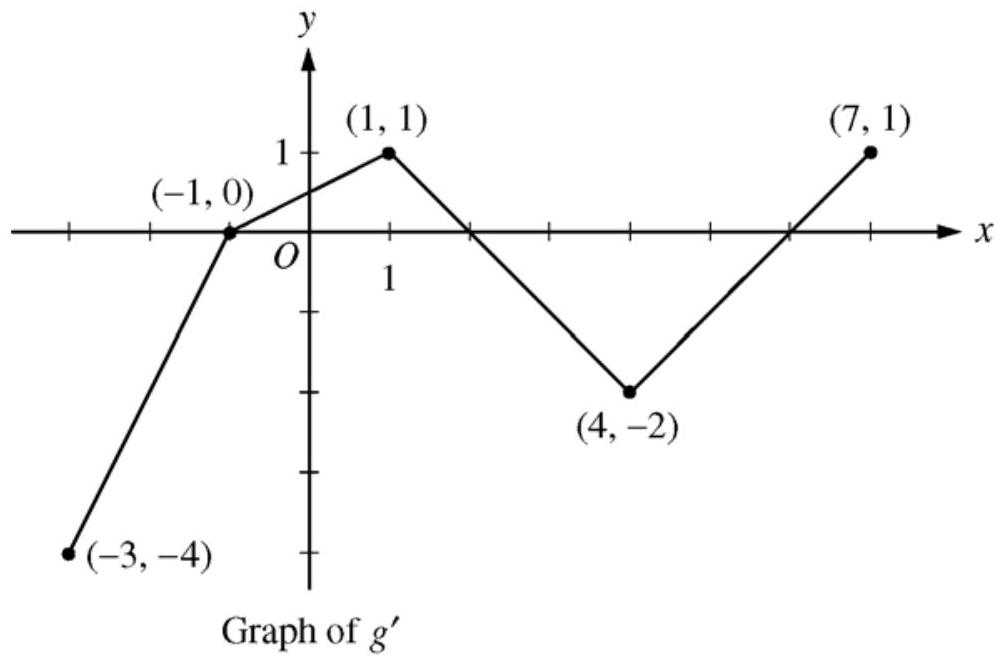
\includegraphics[width=0.6\linewidth]{figures/bc-2008-form-b_fig1.jpg}
\end{center}
Let $g$ be a continuous function with $g(2)=5$. The graph of the piecewise-linear function $g^{\prime}$, the derivative of $g$, is shown above for $-3 \leq x \leq 7$.\\
\begin{parts}
\part Find the $x$-coordinate of all points of inflection of the graph of $y=g(x)$ for $-3<x<7$. Justify your answer.
\part Find the absolute maximum value of $g$ on the interval $-3 \leq x \leq 7$. Justify your answer.
\part Find the average rate of change of $g(x)$ on the interval $-3 \leq x \leq 7$.
\part Find the average rate of change of $g^{\prime}(x)$ on the interval $-3 \leq x \leq 7$. Does the Mean Value Theorem applied on the interval $-3 \leq x \leq 7$ guarantee a value of $c$, for $-3<c<7$, such that $g^{\prime \prime}(c)$ is equal to this average rate of change? Why or why not?
\end{parts}
\begin{solution}
\begin{parts}
\part $g^{\prime}$ changes from increasing to decreasing at $x=1$; $g^{\prime}$ changes from decreasing to increasing at $x=4$.

Points of inflection for the graph of $y=g(x)$ occur at $x=1$ and $x=4$.
\part The only sign change of $g^{\prime}$ from positive to negative in the interval is at $x=2$.

\[\begin{aligned}
g(-3) & =5+\int_{2}^{-3} g^{\prime}(x) d x=5+\left(-\frac{3}{2}\right)+4=\frac{15}{2} \\
g(2) & =5 \\
g(7) & =5+\int_{2}^{7} g^{\prime}(x) d x=5+(-4)+\frac{1}{2}=\frac{3}{2}
\end{aligned}\]

The maximum value of $g$ for $-3 \leq x \leq 7$ is $\frac{15}{2}$.
\part $\frac{g(7)-g(-3)}{7-(-3)}=\frac{\frac{3}{2}-\frac{15}{2}}{10}=-\frac{3}{5}$
\part $\frac{g^{\prime}(7)-g^{\prime}(-3)}{7-(-3)}=\frac{1-(-4)}{10}=\frac{1}{2}$

No, the MVT does not guarantee the existence of a value $c$ with the stated properties because $g^{\prime}$ is not differentiable for at least one point in $-3<x<7$.
\end{parts}
\par\medskip
\textbf{Rubric:}\par
\begin{parts}
\part $2:\left\{\begin{array}{l}
1: x \text {-values } \\
1: \text { justification }
\end{array}\right.$
\part $3:\left\{\begin{array}{l}
1: \text { identifies } x=2 \text { as a candidate } \\
1: \text { considers endpoints } \\
1: \text { maximum value and justification }
\end{array}\right.$
\part $2:\left\{\begin{array}{l}
1: \text { difference quotient } \\
1: \text { answer }
\end{array}\right.$
\part $2:\left\{\begin{array}{l}
1: \text { average value of } g^{\prime}(x) \\
1: \text { answer "No" with reason }
\end{array}\right.$
\end{parts}
\end{solution}

\question
% Q6 | 2008 Calculus BC Form B | Part B | Calculator Prohibited
Let $f$ be the function given by $f(x)=\frac{2 x}{1+x^{2}}$.\\
\begin{parts}
\part Write the first four nonzero terms and the general term of the Taylor series for $f$ about $x=0$.
\part Does the series found in part (a), when evaluated at $x=1$, converge to $f(1)$ ? Explain why or why not.
\part The derivative of $\ln \left(1+x^{2}\right)$ is $\frac{2 x}{1+x^{2}}$. Write the first four nonzero terms of the Taylor series for $\ln \left(1+x^{2}\right)$ about $x=0$.
\part Use the series found in part (c) to find a rational number $A$ such that $\left|A-\ln \left(\frac{5}{4}\right)\right|<\frac{1}{100}$. Justify your answer.
\end{parts}
\begin{solution}
\begin{parts}
\part $\frac{1}{1-u}=1+u+u^{2}+\cdots+u^{n}+\cdots$

\[\begin{aligned}
& \frac{1}{1+x^{2}}=1-x^{2}+x^{4}-x^{6}+\cdots+\left(-x^{2}\right)^{n}+\cdots \\
& \frac{2 x}{1+x^{2}}=2 x-2 x^{3}+2 x^{5}-2 x^{7}+\cdots+(-1)^{n} 2 x^{2 n+1}+\cdots
\end{aligned}\]
\part No, the series does not converge when $x=1$ because when $x=1$, the terms of the series do not converge to 0 .
\part $\ln \left(1+x^{2}\right)=\int_{0}^{x} \frac{2 t}{1+t^{2}} d t$

\[\begin{aligned}
& =\int_{0}^{x}\left(2 t-2 t^{3}+2 t^{5}-2 t^{7}+\cdots\right) d t \\
& =x^{2}-\frac{1}{2} x^{4}+\frac{1}{3} x^{6}-\frac{1}{4} x^{8}+\cdots
\end{aligned}\]
\part $\ln \left(\frac{5}{4}\right)=\ln \left(1+\frac{1}{4}\right)=\left(\frac{1}{2}\right)^{2}-\frac{1}{2}\left(\frac{1}{2}\right)^{4}+\frac{1}{3}\left(\frac{1}{2}\right)^{6}-\frac{1}{4}\left(\frac{1}{2}\right)^{8}+\cdots$ Let $A=\left(\frac{1}{2}\right)^{2}-\left(\frac{1}{2}\right)\left(\frac{1}{2}\right)^{4}=\frac{7}{32}$.\\
Since the series is a converging alternating series and the absolute values of the individual terms decrease to 0 , $\left|A-\ln \left(\frac{5}{4}\right)\right|<\left|\frac{1}{3}\left(\frac{1}{2}\right)^{6}\right|=\frac{1}{3} \cdot \frac{1}{64}<\frac{1}{100}$.
\end{parts}
\par\medskip
\textbf{Rubric:}\par
\begin{parts}
\part $3:\left\{\begin{array}{l}
1: \text { two of the first four terms } \\
1: \text { remaining terms } \\
1: \text { general term }
\end{array}\right.$
\part 1 : answer with reason
\part $2:\left\{\begin{array}{l}1: \text { two of the first four terms } \\ 1: \text { remaining terms }\end{array}\right.$
\part $3:\left\{\begin{array}{l}1: \text { uses } x=\frac{1}{2} \\ 1: \text { value of } A \\ 1: \text { justification }\end{array}\right.$
\end{parts}
\end{solution}

\end{questions}

\section*{2009 AP Calculus BC}

\begin{questions}

\question
% Q1 | 2009 Calculus BC | Part A | Calculator Active
\begin{center}
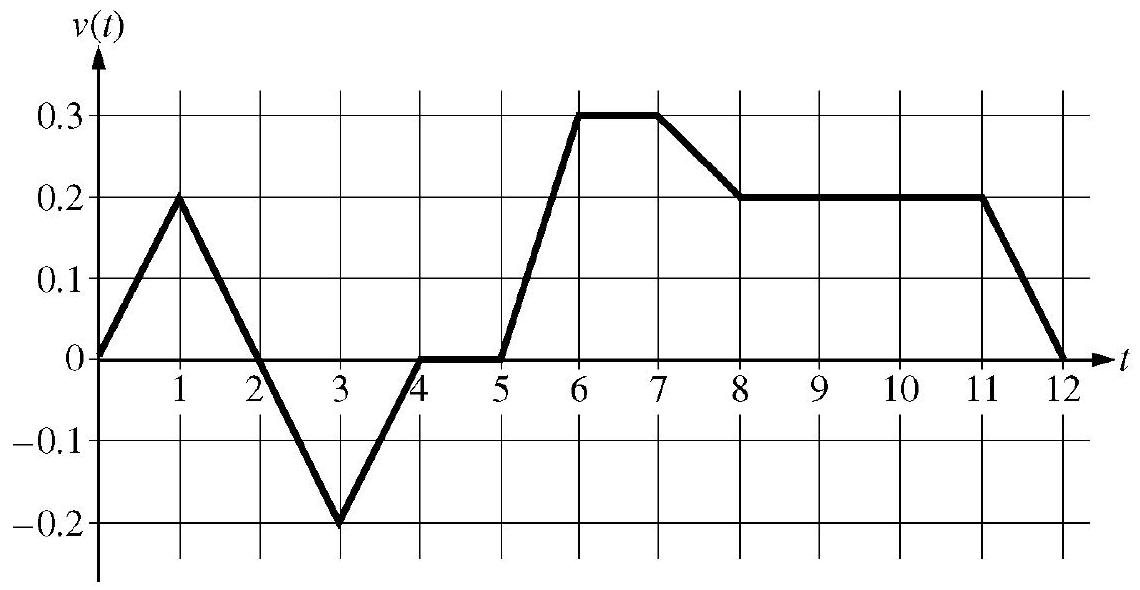
\includegraphics[width=0.6\linewidth]{figures/bc-2009_fig1.jpg}
\end{center}
Caren rides her bicycle along a straight road from home to school, starting at home at time $t=0$ minutes and arriving at school at time $t=12$ minutes. During the time interval $0 \leq t \leq 12$ minutes, her velocity $v(t)$, in miles per minute, is modeled by the piecewise-linear function whose graph is shown above.\\
\begin{parts}
\part Find the acceleration of Caren's bicycle at time $t=7.5$ minutes. Indicate units of measure.
\part Using correct units, explain the meaning of $\int_{0}^{12}|v(t)| d t$ in terms of Caren's trip. Find the value of $\int_{0}^{12}|v(t)| d t$.
\part Shortly after leaving home, Caren realizes she left her calculus homework at home, and she returns to get it. At what time does she turn around to go back home? Give a reason for your answer.
\part Larry also rides his bicycle along a straight road from home to school in 12 minutes. His velocity is modeled by the function $w$ given by $w(t)=\frac{\pi}{15} \sin \left(\frac{\pi}{12} t\right)$, where $w(t)$ is in miles per minute for $0 \leq t \leq 12$ minutes. Who lives closer to school: Caren or Larry? Show the work that leads to your answer.
\end{parts}
\begin{solution}
\begin{parts}
\part $a(7.5)=v^{\prime}(7.5)=\frac{v(8)-v(7)}{8-7}=-0.1 \mathrm{miles} / \mathrm{minute}^{2}$
\part $\quad \int_{0}^{12}|v(t)| d t$ is the total distance, in miles, that Caren rode during the 12 minutes from $t=0$ to $t=12$.

\begin{align*}\int_{0}^{12}|v(t)| d t & =\int_{0}^{2} v(t) d t-\int_{2}^{4} v(t) d t+\int_{4}^{12} v(t) d t \\
& =0.2+0.2+1.4=1.8 \mathrm{miles}\end{align*}
\part Caren turns around to go back home at time $t=2$ minutes. This is the time at which her velocity changes from positive to negative.
\part $\quad \int_{0}^{12} w(t) d t=1.6$; Larry lives 1.6 miles from school.\\
$\int_{0}^{12} v(t) d t=1.4$; Caren lives 1.4 miles from school.\\
Therefore, Caren lives closer to school.
\end{parts}
\par\medskip
\textbf{Rubric:}\par
\begin{parts}
\part $2:\left\{\begin{array}{l}1: \text { answer } \\ 1: \text { units }\end{array}\right.$
\part $2:\left\{\begin{array}{l}1: \text { meaning of integral } \\ 1: \text { value of integral }\end{array}\right.$
\part $2:\left\{\begin{array}{l}1: \text { answer } \\ 1: \text { reason }\end{array}\right.$
\part $3:\left\{\begin{array}{l}2: \text { Larry's distance from school } \\ 1: \text { integral } \\ 1: \text { value } \\ 1: \text { Caren's distance from school } \\ \text { and conclusion }\end{array}\right.$
\end{parts}
\end{solution}

\question
% Q2 | 2009 Calculus BC | Part A | Calculator Active
The rate at which people enter an auditorium for a rock concert is modeled by the function $R$ given by $R(t)=1380 t^{2}-675 t^{3}$ for $0 \leq t \leq 2$ hours; $R(t)$ is measured in people per hour. No one is in the auditorium at time $t=0$, when the doors open. The doors close and the concert begins at time $t=2$.\\
\begin{parts}
\part How many people are in the auditorium when the concert begins?
\part Find the time when the rate at which people enter the auditorium is a maximum. Justify your answer.
\part The total wait time for all the people in the auditorium is found by adding the time each person waits, starting at the time the person enters the auditorium and ending when the concert begins. The function $w$ models the total wait time for all the people who enter the auditorium before time $t$. The derivative of $w$ is given by $w^{\prime}(t)=(2-t) R(t)$. Find $w(2)-w(1)$, the total wait time for those who enter the auditorium after time $t=1$.
\part On average, how long does a person wait in the auditorium for the concert to begin? Consider all people who enter the auditorium after the doors open, and use the model for total wait time from part (c).
\end{parts}
\begin{solution}
\begin{parts}
\part $\int_{0}^{2} R(t) d t=980$ people
\part $\quad R^{\prime}(t)=0$ when $t=0$ and $t=1.36296$

The maximum rate may occur at $0, a=1.36296$, or 2 .

\begin{align*}& R(0)=0 \\
& R(a)=854.527 \\
& R(2)=120\end{align*}

The maximum rate occurs when $t=1.362$ or 1.363.
\part $\quad w(2)-w(1)=\int_{1}^{2} w^{\prime}(t) d t=\int_{1}^{2}(2-t) R(t) d t=387.5$

The total wait time for those who enter the auditorium after time $t=1$ is 387.5 hours.
\part $\frac{1}{980} w(2)=\frac{1}{980} \int_{0}^{2}(2-t) R(t) d t=0.77551$

On average, a person waits 0.775 or 0.776 hour.
\end{parts}
\par\medskip
\textbf{Rubric:}\par
\begin{parts}
\part $2:\left\{\begin{array}{l}1: \text { integral } \\ 1: \text { answer }\end{array}\right.$
\part $2:\left\{\begin{array}{l}
1: \text { integral } \\
1: \text { answer }
\end{array}\right.$
\end{parts}
\end{solution}

\question
% Q3 | 2009 Calculus BC | Part A | Calculator Active
\begin{center}
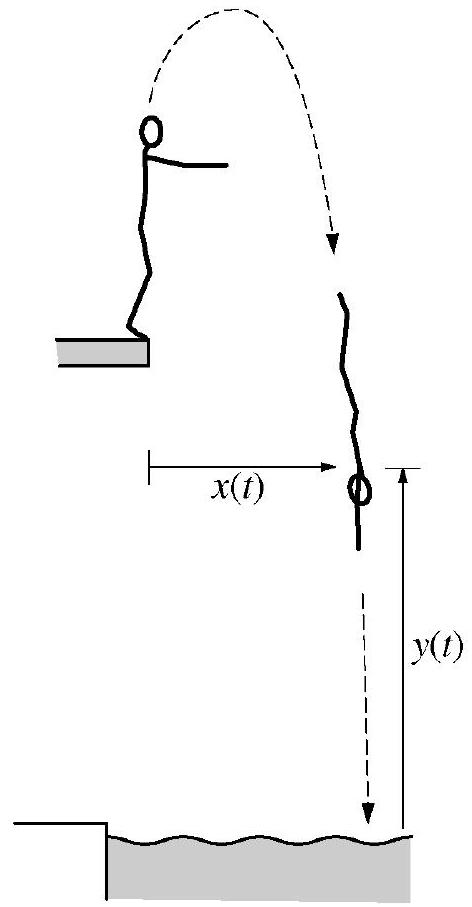
\includegraphics[width=0.6\linewidth]{figures/bc-2009_fig2.jpg}
\end{center}

Note: Figure not drawn to scale.\\
A diver leaps from the edge of a diving platform into a pool below. The figure above shows the initial position of the diver and her position at a later time. At time $t$ seconds after she leaps, the horizontal distance from the front edge of the platform to the diver's shoulders is given by $x(t)$, and the vertical distance from the water surface to her shoulders is given by $y(t)$, where $x(t)$ and $y(t)$ are measured in meters. Suppose that the diver's shoulders are 11.4 meters above the water when she makes her leap and that

\[\frac{d x}{d t}=0.8 \text { and } \frac{d y}{d t}=3.6-9.8 t,\]

for $0 \leq t \leq A$, where $A$ is the time that the diver's shoulders enter the water.\\
\begin{parts}
\part Find the maximum vertical distance from the water surface to the diver's shoulders.
\part Find $A$, the time that the diver's shoulders enter the water.
\part Find the total distance traveled by the diver's shoulders from the time she leaps from the platform until the time her shoulders enter the water.
\part Find the angle $\theta, 0<\theta<\frac{\pi}{2}$, between the path of the diver and the water at the instant the diver's shoulders enter the water.
\end{parts}
\begin{solution}
\begin{parts}
\part $\frac{d y}{d t}=0$ only when $t=0.36735$. Let $b=0.36735$.

The maximum vertical distance from the water surface to the diver's shoulders is\\
$y(b)=11.4+\int_{0}^{b} \frac{d y}{d t} d t=12.061$ meters.\\
Alternatively, $y(t)=11.4+3.6 t-4.9 t^{2}$, so $y(b)=12.061$ meters.
\part $y(A)=11.4+\int_{0}^{A} \frac{d y}{d t} d t=11.4+3.6 A-4.9 A^{2}=0$ when $A=1.936$ seconds.
\part $\int_{0}^{A} \sqrt{\left(\frac{d x}{d t}\right)^{2}+\left(\frac{d y}{d t}\right)^{2}} d t=12.946$ meters
\part At time $A, \frac{d y}{d x}=\left.\frac{d y / d t}{d x / d t}\right|_{t=A}=-19.21913$.

The angle between the path of the diver and the water is $\arctan(19.21913) \approx 1.518$ or 1.519 radians.
\end{parts}
\par\medskip
\textbf{Rubric:}\par
\begin{parts}
\part $2:\left\{\begin{array}{l}1: \text { integral } \\ 1: \text { answer }\end{array}\right.$
\part $3:\left\{\begin{array}{l}
1: \text { considers } \frac{d y}{d t}=0 \\
1: \text { integral or } y(t) \\
1: \text { answer }
\end{array}\right.$
\part $2:\left\{\begin{array}{l}1: \text { equation } \\ 1: \text { answer }\end{array}\right.$
\part $2:\left\{\begin{array}{l}1: \frac{d y}{d x} \text { at time } A \\ 1: \text { answer }\end{array}\right.$
\end{parts}
\end{solution}

\question
% Q4 | 2009 Calculus BC | Part B | Calculator Prohibited
Consider the differential equation $\frac{d y}{d x}=6 x^{2}-x^{2} y$. Let $y=f(x)$ be a particular solution to this differential equation with the initial condition $f(-1)=2$.\\
\begin{parts}
\part Use Euler's method with two steps of equal size, starting at $x=-1$, to approximate $f(0)$. Show the work that leads to your answer.
\part At the point $(-1,2)$, the value of $\frac{d^{2} y}{d x^{2}}$ is -12 . Find the second-degree Taylor polynomial for $f$ about $x=-1$.
\part Find the particular solution $y=f(x)$ to the given differential equation with the initial condition $f(-1)=2$.
\end{parts}
\begin{solution}
\begin{parts}
\part $f\left(-\frac{1}{2}\right) \approx f(-1)+\left(\left.\frac{d y}{d x}\right|_{(-1,2)}\right) \cdot \Delta x$

\[=2+4 \cdot \frac{1}{2}=4\]

\[\begin{aligned}
f(0) & \approx f\left(-\frac{1}{2}\right)+\left(\left.\frac{d y}{d x}\right|_{\left(-\frac{1}{2}, 4\right)}\right) \cdot \Delta x \\
& \approx 4+\frac{1}{2} \cdot \frac{1}{2}=\frac{17}{4}
\end{aligned}\]
\part $P_{2}(x)=2+4(x+1)-6(x+1)^{2}$
\part $\frac{d y}{d x}=x^{2}(6-y)$

\[\begin{aligned}
& \int \frac{1}{6-y} d y=\int x^{2} d x \\
& -\ln |6-y|=\frac{1}{3} x^{3}+C \\
& -\ln 4=-\frac{1}{3}+C \\
& C=\frac{1}{3}-\ln 4 \\
& \ln |6-y|=-\frac{1}{3} x^{3}-\left(\frac{1}{3}-\ln 4\right) \\
& |6-y|=4 e^{-\frac{1}{3}\left(x^{3}+1\right)} \\
& y=6-4 e^{-\frac{1}{3}\left(x^{3}+1\right)}
\end{aligned}\]
\end{parts}
\par\medskip
\textbf{Rubric:}\par
\begin{parts}
\part $2:\left\{\begin{array}{l}
1: \text { Euler's method with two steps } \\
1: \text { answer }
\end{array}\right.$
\part 1 : answer
\part $6:\left\{\begin{array}{l}
1: \text { separation of variables } \\
2: \text { antiderivatives } \\
1: \text { constant of integration } \\
1: \text { uses initial condition } \\
1: \text { solves for } y
\end{array}\right.$
\part Note: max 3/6 [1-2-0-0-0] if no constant of integration
\part Note: $0 / 6$ if no separation of variables
\end{parts}
\end{solution}

\question
% Q5 | 2009 Calculus BC | Part B | Calculator Prohibited
\begin{center}
\begin{tabular}{|c|c|c|c|c|c|}
\hline
$x$ & 2 & 3 & 5 & 8 & 13 \\
\hline
$f(x)$ & 1 & 4 & -2 & 3 & 6 \\
\hline
\end{tabular}
\end{center}
Let $f$ be a function that is twice differentiable for all real numbers. The table above gives values of $f$ for selected points in the closed interval $2 \leq x \leq 13$.\\
\begin{parts}
\part Estimate $f^{\prime}(4)$. Show the work that leads to your answer.
\part Evaluate $\int_{2}^{13}\left(3-5 f^{\prime}(x)\right) d x$. Show the work that leads to your answer.
\part Use a left Riemann sum with subintervals indicated by the data in the table to approximate $\int_{2}^{13} f(x) d x$. Show the work that leads to your answer.
\part Suppose $f^{\prime}(5)=3$ and $f^{\prime \prime}(x)<0$ for all $x$ in the closed interval $5 \leq x \leq 8$. Use the line tangent to the graph of $f$ at $x=5$ to show that $f(7) \leq 4$. Use the secant line for the graph of $f$ on $5 \leq x \leq 8$ to show that $f(7) \geq \frac{4}{3}$.
\end{parts}
\begin{solution}
\begin{parts}
\part $f^{\prime}(4) \approx \frac{f(5)-f(3)}{5-3}=-3$
\part $\int_{2}^{13}\left(3-5 f^{\prime}(x)\right) d x=\int_{2}^{13} 3 d x-5 \int_{2}^{13} f^{\prime}(x) d x$

\[=3(13-2)-5(f(13)-f(2))=8\]
\part $\int_{2}^{13} f(x) d x \approx f(2)(3-2)+f(3)(5-3)$

\[+f(5)(8-5)+f(8)(13-8)=18\]
\part An equation for the tangent line is $y=-2+3(x-5)$. Since $f^{\prime \prime}(x)<0$ for all $x$ in the interval $5 \leq x \leq 8$, the line tangent to the graph of $y=f(x)$ at $x=5$ lies above the graph for all $x$ in the interval $5<x \leq 8$.

Therefore, $f(7) \leq-2+3 \cdot 2=4$.\\
An equation for the secant line is $y=-2+\frac{5}{3}(x-5)$. Since $f^{\prime \prime}(x)<0$ for all $x$ in the interval $5 \leq x \leq 8$, the secant line connecting (5, $f(5)$ ) and (8, $f(8)$ ) lies below the graph of $y=f(x)$ for all $x$ in the interval $5<x<8$. Therefore, $f(7) \geq-2+\frac{5}{3} \cdot 2=\frac{4}{3}$.
\end{parts}
\par\medskip
\textbf{Rubric:}\par
\begin{parts}
\part 1 : answer $2:\left\{\begin{array}{l}1: \text { uses Fundamental Theorem } \\ \quad \text { of Calculus } \\ 1: \text { answer }\end{array}\right. 2:\left\{\begin{array}{l}1: \text { left Riemann sum } \\ 1: \text { answer }\end{array}\right. 4:\left\{\begin{array}{l}1: \text { tangent line } \\ 1: \text { shows } f(7) \leq 4 \\ 1: \text { secant line } \\ 1: \text { shows } f(7) \geq \frac{4}{3}\end{array}\right.$
\end{parts}
\end{solution}

\question
% Q6 | 2009 Calculus BC | Part B | Calculator Prohibited
The Maclaurin series for $e^{x}$ is $e^{x}=1+x+\frac{x^{2}}{2}+\frac{x^{3}}{6}+\cdots+\frac{x^{n}}{n!}+\cdots$. The continuous function $f$ is defined by $f(x)=\frac{e^{(x-1)^{2}}-1}{(x-1)^{2}}$ for $x \neq 1$ and $f(1)=1$. The function $f$ has derivatives of all orders at $x=1$.\\
\begin{parts}
\part Write the first four nonzero terms and the general term of the Taylor series for $e^{(x-1)^{2}}$ about $x=1$.
\part Use the Taylor series found in part (a) to write the first four nonzero terms and the general term of the Taylor series for $f$ about $x=1$.
\part Use the ratio test to find the interval of convergence for the Taylor series found in part (b).
\part Use the Taylor series for $f$ about $x=1$ to determine whether the graph of $f$ has any points of inflection.
\end{parts}
\begin{solution}
\begin{parts}
\part $1+(x-1)^{2}+\frac{(x-1)^{4}}{2}+\frac{(x-1)^{6}}{6}+\cdots+\frac{(x-1)^{2 n}}{n!}+\cdots$
\part $1+\frac{(x-1)^{2}}{2}+\frac{(x-1)^{4}}{6}+\frac{(x-1)^{6}}{24}+\cdots+\frac{(x-1)^{2 n}}{(n+1)!}+\cdots$
\part $\lim _{n \rightarrow \infty}\left|\frac{\frac{(x-1)^{2 n+2}}{(n+2)!}}{\frac{(x-1)^{2 n}}{(n+1)!}}\right|=\lim _{n \rightarrow \infty} \frac{(n+1)!}{(n+2)!}(x-1)^{2}=\lim _{n \rightarrow \infty} \frac{(x-1)^{2}}{n+2}=0$ Therefore, the interval of convergence is $(-\infty, \infty)$.
\part $f^{\prime \prime}(x)=1+\frac{4 \cdot 3}{6}(x-1)^{2}+\frac{6 \cdot 5}{24}(x-1)^{4}+\cdots$

\[+\frac{2 n(2 n-1)}{(n+1)!}(x-1)^{2 n-2}+\cdots\]

Since every term of this series is nonnegative, $f^{\prime \prime}(x) \geq 0$ for all $x$. Therefore, the graph of $f$ has no points of inflection.
\end{parts}
\par\medskip
\textbf{Rubric:}\par
\begin{parts}
\part $2:\left\{\begin{array}{l}
1: \text { first four terms } \\
1: \text { general term }
\end{array}\right.$
\part $2:\left\{\begin{array}{l}
1: \text { first four terms } \\
1: \text { general term }
\end{array}\right.$
\part $3:\left\{\begin{array}{l}
1: \text { sets up ratio } \\
1: \text { computes limit of ratio } \\
1: \text { answer }
\end{array}\right.$
\part $2:\left\{\begin{array}{l}
1: f^{\prime \prime}(x) \\
1: \text { answer }
\end{array}\right.$
\end{parts}
\end{solution}

\end{questions}

\section*{2009 AP Calculus BC Form B}

\begin{questions}

\question
% Q1 | 2009 Calculus BC Form B | Part A | Calculator Active
\begin{center}
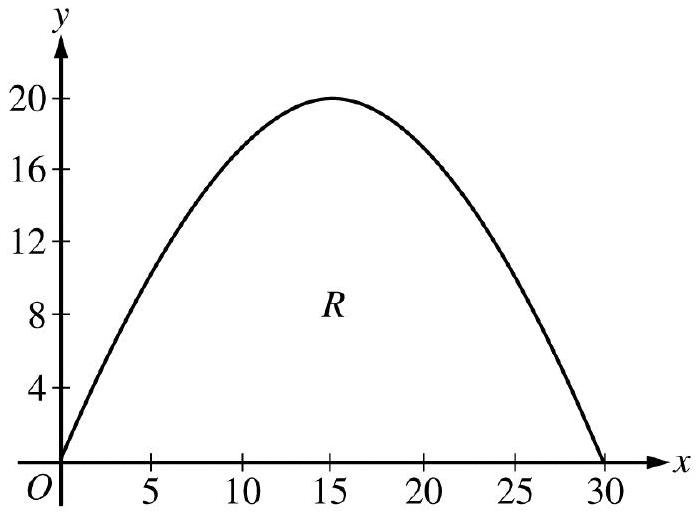
\includegraphics[width=0.6\linewidth]{figures/bc-2009-form-b_fig1.jpg}
\end{center}
A baker is creating a birthday cake. The base of the cake is the region $R$ in the first quadrant under the graph of $y=f(x)$ for $0 \leq x \leq 30$, where $f(x)=20 \sin \left(\frac{\pi x}{30}\right)$. Both $x$ and $y$ are measured in centimeters. The region $R$ is shown in the figure above. The derivative of $f$ is $f^{\prime}(x)=\frac{2 \pi}{3} \cos \left(\frac{\pi x}{30}\right)$.\\
\begin{parts}
\part The region $R$ is cut out of a 30 -centimeter-by-20-centimeter rectangular sheet of cardboard, and the remaining cardboard is discarded. Find the area of the discarded cardboard.
\part The cake is a solid with base $R$. Cross sections of the cake perpendicular to the $x$-axis are semicircles. If the baker uses 0.05 gram of unsweetened chocolate for each cubic centimeter of cake, how many grams of unsweetened chocolate will be in the cake?
\part Find the perimeter of the base of the cake.
\end{parts}
\begin{solution}
\begin{parts}
\part Area $=30 \cdot 20-\int_{0}^{30} f(x) d x=218.028 \mathrm{~cm}^{2}$

\[3:\left\{\begin{array}{l}
2: \text { integral } \\
1: \text { answer }
\end{array}\right.\]
\part Volume $=\int_{0}^{30} \frac{\pi}{2}\left(\frac{f(x)}{2}\right)^{2} d x=2356.194 \mathrm{~cm}^{3}$

Therefore, the baker needs $2356.194 \times 0.05=117.809$ or 117.810 grams

\[3:\left\{\begin{array}{l}
2: \text { integral } \\
1: \text { answer }
\end{array}\right.\]

of chocolate.
\part Perimeter $=30+\int_{0}^{30} \sqrt{1+\left(f^{\prime}(x)\right)^{2}} d x=81.803$ or 81.804 cm
\end{parts}
\par\medskip
\textbf{Rubric:}\par
\begin{parts}
\part $3:\left\{\begin{array}{l}
2: \text { integral } \\
1: \text { answer }
\end{array}\right.$
\end{parts}
\end{solution}

\question
% Q2 | 2009 Calculus BC Form B | Part A | Calculator Active
A storm washed away sand from a beach, causing the edge of the water to get closer to a nearby road. The rate at which the distance between the road and the edge of the water was changing during the storm is modeled by $f(t)=\sqrt{t}+\cos t-3$ meters per hour, $t$ hours after the storm began. The edge of the water was 35 meters from the road when the storm began, and the storm lasted 5 hours. The derivative of $f(t)$ is $f^{\prime}(t)=\frac{1}{2 \sqrt{t}}-\sin t$.\\

\begin{center}
  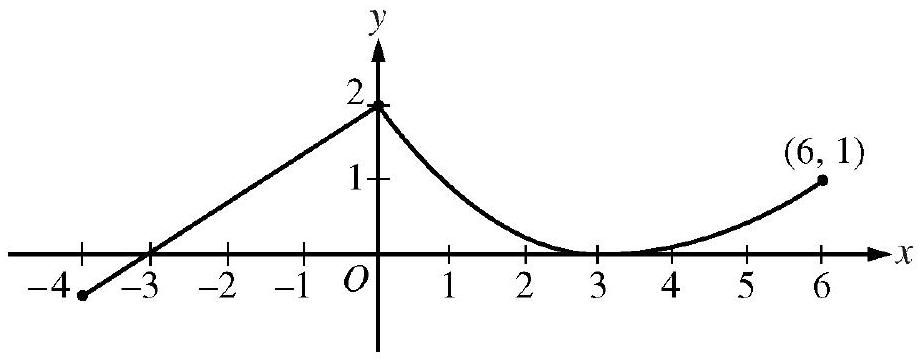
\includegraphics[width=0.6\linewidth]{figures/bc-2009-form-b_fig2.jpg}
\end{center}
\begin{parts}
\part What was the distance between the road and the edge of the water at the end of the storm?
\part Using correct units, interpret the value $f^{\prime}(4)=1.007$ in terms of the distance between the road and the edge of the water.
\part At what time during the 5 hours of the storm was the distance between the road and the edge of the water decreasing most rapidly? Justify your answer.
\part After the storm, a machine pumped sand back onto the beach so that the distance between the road and the edge of the water was growing at a rate of $g(p)$ meters per day, where $p$ is the number of days since pumping began. Write an equation involving an integral expression whose solution would give the number of days that sand must be pumped to restore the original distance between the road and the edge of the water.
\end{parts}
\begin{solution}
\begin{parts}
\part $35+\int_{0}^{5} f(t) d t=26.494$ or 26.495 meters
\part Four hours after the storm began, the rate of change of the distance between the road and the edge of the water is increasing at a rate of 1.007 meters/hours ${ }^{2}$.
\part $\quad f^{\prime}(t)=0$ when $t=0.66187$ and $t=2.84038$ The minimum of $f$ for $0 \leq t \leq 5$ may occur at 0 , 0.66187, 2.84038, or 5.

\begin{align*}& f(0)=-2 \\
& f(0.66187)=-1.39760 \\
& f(2.84038)=-2.26963 \\
& f(5)=-0.48027\end{align*}

The distance between the road and the edge of the water was decreasing most rapidly at time $t=2.840$ hours after the storm began.
\part $-\int_{0}^{5} f(t) d t=\int_{0}^{x} g(p) d p$
\end{parts}
\par\medskip
\textbf{Rubric:}\par
\begin{parts}
\part $2:\left\{\begin{array}{l}
1: \text { integral } \\
1: \text { answer }
\end{array}\right.$
\part $2:\left\{\begin{array}{l}1: \text { interpretation of } f^{\prime}(4) \\ 1: \text { units }\end{array}\right.$
\part $3:\left\{\begin{array}{l}
1: \text { considers } f^{\prime}(t)=0 \\
1: \text { answer } \\
1: \text { justification }
\end{array}\right.$
\part $2:\left\{\begin{array}{l}
1: \text { integral of } g \\
1: \text { answer }
\end{array}\right.$
\end{parts}
\end{solution}

\question
% Q3 | 2009 Calculus BC Form B | Part A | Calculator Active
A continuous function $f$ is defined on the closed interval $-4 \leq x \leq 6$. The graph of $f$ consists of a line segment and a curve that is tangent to the $x$-axis at $x=3$, as shown in the figure below. On the interval $0<x<6$, the function $f$ is twice differentiable, with $f^{\prime \prime}(x)>0$.\\
\begin{parts}
\part Is $f$ differentiable at $x=0$ ? Use the definition of the derivative with one-sided limits to justify your answer.
\part For how many values of $a,-4 \leq a<6$, is the average rate of change of $f$ on the interval $[a, 6]$ equal to 0 ? Give a reason for your answer.
\part Is there a value of $a,-4 \leq a<6$, for which the Mean Value Theorem, applied to the interval $[a, 6]$, guarantees a value $c, a<c<6$, at which $f^{\prime}(c)=\frac{1}{3}$ ? Justify your answer.
\part The function $g$ is defined by $g(x)=\int_{0}^{x} f(t) d t$ for $-4 \leq x \leq 6$. On what intervals contained in $[-4,6]$ is the graph of $g$ concave up? Explain your reasoning.
\end{parts}
\begin{solution}
\begin{parts}
\part $\lim _{h \rightarrow 0^{-}} \frac{f(h)-f(0)}{h}=\frac{2}{3}$\\
$\lim _{h \rightarrow 0^{+}} \frac{f(h)-f(0)}{h}<0$\\
Since the one-sided limits do not agree, $f$ is not differentiable at $x=0$.
\part $\frac{f(6)-f(a)}{6-a}=0$ when $f(a)=f(6)$. There are two values of $a$ for which this is true.
\part Yes, $a=3$. The function $f$ is differentiable on the interval $3<x<6$ and continuous on $3 \leq x \leq 6$.\\
Also, $\frac{f(6)-f(3)}{6-3}=\frac{1-0}{6-3}=\frac{1}{3}$.\\
By the Mean Value Theorem, there is a value $c$, $3<c<6$, such that $f^{\prime}(c)=\frac{1}{3}$.
\part $g^{\prime}(x)=f(x), g^{\prime \prime}(x)=f^{\prime}(x) g^{\prime \prime}(x)>0$ when $f^{\prime}(x)>0$\\
This is true for $-4<x<0$ and $3<x<6$.
\end{parts}
\par\medskip
\textbf{Rubric:}\par
\begin{parts}
\part $2:\left\{\begin{array}{l}1: \text { sets up difference quotient at } x=0 \\ 1: \text { answer with justification }\end{array}\right.$
\part $2:\left\{\begin{array}{l}1: \text { expression for average rate of change } \\ 1: \text { answer with reason }\end{array}\right.$
\part $2:\left\{\begin{array}{l}1: \text { answers "yes" and identifies } a=3 \\ 1: \text { justification }\end{array}\right.$
\part $3:\left\{\begin{array}{l}1: g^{\prime}(x)=f(x) \\ 1: \text { considers } g^{\prime \prime}(x)>0 \\ 1: \text { answer }\end{array}\right.$
\end{parts}
\end{solution}

\question
% Q4 | 2009 Calculus BC Form B | Part B | Calculator Prohibited
\begin{center}
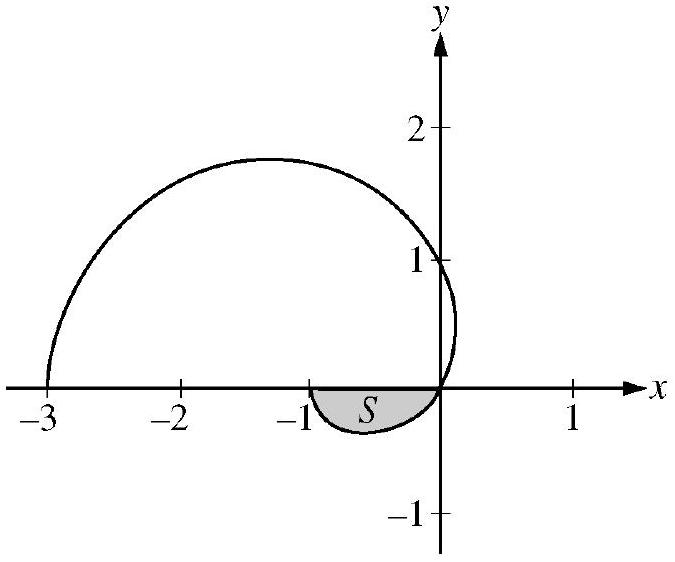
\includegraphics[width=0.6\linewidth]{figures/bc-2009-form-b_fig3.jpg}
\end{center}
The graph of the polar curve $r=1-2 \cos \theta$ for $0 \leq \theta \leq \pi$ is shown above. Let $S$ be the shaded region in the third quadrant bounded by the curve and the $x$-axis.\\

\begin{center}
  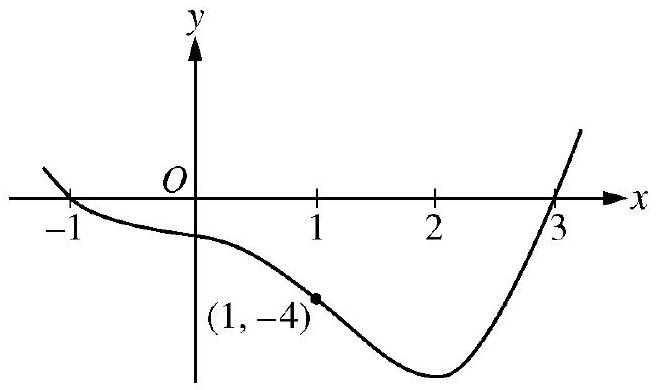
\includegraphics[width=0.6\linewidth]{figures/bc-2009-form-b_fig4.jpg}
\end{center}
\begin{parts}
\part Write an integral expression for the area of $S$.
\part Write expressions for $\frac{d x}{d \theta}$ and $\frac{d y}{d \theta}$ in terms of $\theta$.
\part Write an equation in terms of $x$ and $y$ for the line tangent to the graph of the polar curve at the point where $\theta=\frac{\pi}{2}$. Show the computations that lead to your answer.
\end{parts}
\begin{solution}
\begin{parts}
\part $\quad r(0)=-1 ; \quad r(\theta)=0$ when $\theta=\frac{\pi}{3}$.

Area of $S=\frac{1}{2} \int_{0}^{\pi / 3}(1-2 \cos \theta)^{2} d \theta$
\part $x=r \cos \theta$ and $y=r \sin \theta$

\begin{align*}& \frac{d r}{d \theta}=2 \sin \theta \\
& \frac{d x}{d \theta}=\frac{d r}{d \theta} \cos \theta-r \sin \theta=4 \sin \theta \cos \theta-\sin \theta \\
& \frac{d y}{d \theta}=\frac{d r}{d \theta} \sin \theta+r \cos \theta=2 \sin ^{2} \theta+(1-2 \cos \theta) \cos \theta\end{align*}
\part When $\theta=\frac{\pi}{2}$, we have $x=0, y=1$.

\[\left.\frac{d y}{d x}\right|_{\theta=\frac{\pi}{2}}=\left.\frac{d y / d \theta}{d x / d \theta}\right|_{\theta=\frac{\pi}{2}}=-2\]

The tangent line is given by $y=1-2 x$.
\end{parts}
\par\medskip
\textbf{Rubric:}\par
\begin{parts}
\part $2:\left\{\begin{array}{l}1: \text { limits and constant } \\ 1: \text { integrand }\end{array}\right.$
\part 4: $\left\{\begin{array}{l}1: \text { uses } x=r \cos \theta \text { and } y=r \sin \theta \\ 1: \frac{d r}{d \theta} \\ 2: \text { answer }\end{array}\right.$
\part $3:\left\{\begin{array}{l}1: \text { values for } x \text { and } y \\ 1: \text { expression for } \frac{d y}{d x} \\ 1: \text { tangent line equation }\end{array}\right.$
\end{parts}
\end{solution}

\question
% Q5 | 2009 Calculus BC Form B | Part B | Calculator Prohibited
Let $f$ be a twice-differentiable function defined on the interval $-1.2<x<3.2$ with $f(1)=2$. The graph of $f^{\prime}$, the derivative of $f$, is shown below. The graph of $f^{\prime}$ crosses the $x$-axis at $x=-1$ and $x=3$ and has a horizontal tangent at $x=2$. Let $g$ be the function given by $g(x)=e^{f(x)}$.\\
\begin{parts}
\part Write an equation for the line tangent to the graph of $g$ at $x=1$.
\part For $-1.2<x<3.2$, find all values of $x$ at which $g$ has a local maximum. Justify your answer.
\part The second derivative of $g$ is $g^{\prime \prime}(x)=e^{f(x)}\left[\left(f^{\prime}(x)\right)^{2}+f^{\prime \prime}(x)\right]$. Is $g^{\prime \prime}(-1)$ positive, negative, or zero? Justify your answer.
\part Find the average rate of change of $g^{\prime}$, the derivative of $g$, over the interval $[1,3]$.
\end{parts}
\begin{solution}
\begin{parts}
\part $g(1)=e^{f(1)}=e^{2}$\\
$g^{\prime}(x)=e^{f(x)} f^{\prime}(x), \quad g^{\prime}(1)=e^{f(1)} f^{\prime}(1)=-4 e^{2}$\\
The tangent line is given by $y=e^{2}-4 e^{2}(x-1)$.
\part $g^{\prime}(x)=e^{f(x)} f^{\prime}(x)$\\
$e^{f(x)}>0$ for all $x$\\
So, $g^{\prime}$ changes from positive to negative only when $f^{\prime}$ changes from positive to negative. This occurs at $x=-1$ only. Thus, $g$ has a local maximum at $x=-1$.
\part $g^{\prime \prime}(-1)=e^{f(-1)}\left[\left(f^{\prime}(-1)\right)^{2}+f^{\prime \prime}(-1)\right] e^{f(-1)}>0$ and $f^{\prime}(-1)=0$\\
Since $f^{\prime}$ is decreasing on a neighborhood of -1 , $f^{\prime \prime}(-1)<0$. Therefore, $g^{\prime \prime}(-1)<0$.
\part $\frac{g^{\prime}(3)-g^{\prime}(1)}{3-1}=\frac{e^{f(3)} f^{\prime}(3)-e^{f(1)} f^{\prime}(1)}{2}=2 e^{2}$
\end{parts}
\par\medskip
\textbf{Rubric:}\par
\begin{parts}
\part $3:\left\{\begin{array}{l}1: g^{\prime}(x) \\ 1: g(1) \text { and } g^{\prime}(1) \\ 1: \text { tangent line equation }\end{array}\right.$
\part $2:\left\{\begin{array}{l}1: \text { answer } \\ 1: \text { justification }\end{array}\right.$
\part $2:\left\{\begin{array}{l}1: \text { answer } \\ 1: \text { justification }\end{array}\right.$
\part $2:\left\{\begin{array}{l}1: \text { difference quotient } \\ 1: \text { answer }\end{array}\right.$
\end{parts}
\end{solution}

\question
% Q6 | 2009 Calculus BC Form B | Part B | Calculator Prohibited
The function $f$ is defined by the power series
\[f(x)=1+(x+1)+(x+1)^{2}+\cdots+(x+1)^{n}+\cdots=\sum_{n=0}^{\infty}(x+1)^{n}\]

for all real numbers $x$ for which the series converges.\\
\begin{parts}
\part Find the interval of convergence of the power series for $f$. Justify your answer.
\part The power series above is the Taylor series for $f$ about $x=-1$. Find the sum of the series for $f$.
\part Let $g$ be the function defined by $g(x)=\int_{-1}^{x} f(t) d t$. Find the value of $g\left(-\frac{1}{2}\right)$, if it exists, or explain why $g\left(-\frac{1}{2}\right)$ cannot be determined.
\part Let $h$ be the function defined by $h(x)=f\left(x^{2}-1\right)$. Find the first three nonzero terms and the general term of the Taylor series for $h$ about $x=0$, and find the value of $h\left(\frac{1}{2}\right)$.
\end{parts}
\begin{solution}
\begin{parts}
\part The power series is geometric with ratio $(x+1)$.

The series converges if and only if $|x+1|<1$.\\
Therefore, the interval of convergence is $-2<x<0$.\\
OR

\[\lim _{n \rightarrow \infty}\left|\frac{(x+1)^{n+1}}{(x+1)^{n}}\right|=|x+1|<1 \text { when }-2<x<0\]

At $x=-2$, the series is $\sum_{n=0}^{\infty}(-1)^{n}$, which diverges since the terms do not converge to 0 . At $x=0$, the series is $\sum_{n=0}^{\infty} 1$, which similarly diverges. Therefore, the interval of convergence is $-2<x<0$.
\part Since the series is geometric,

\[f(x)=\sum_{n=0}^{\infty}(x+1)^{n}=\frac{1}{1-(x+1)}=-\frac{1}{x} \text { for }-2<x<0\]
\part $\quad g\left(-\frac{1}{2}\right)=\int_{-1}^{-\frac{1}{2}}-\frac{1}{x} d x=-\left.\ln |x|\right|_{x=-1} ^{x=-\frac{1}{2}}=\ln 2$
\part $h(x)=f\left(x^{2}-1\right)=1+x^{2}+x^{4}+\cdots+x^{2 n}+\cdots$

\[h\left(\frac{1}{2}\right)=f\left(-\frac{3}{4}\right)=\frac{4}{3}\]
\end{parts}
\par\medskip
\textbf{Rubric:}\par
\begin{parts}
\part $3:\left\{\begin{array}{l}1: \text { identifies as geometric } \\ 1:|x+1|<1 \\ 1: \text { interval of convergence }\end{array}\right.$
\part $3:\left\{\begin{array}{l}1: \text { sets up limit of ratio } \\ 1: \text { radius of convergence } \\ 1: \text { interval of convergence }\end{array}\right.$
\part 1 : answer
\part $2:\left\{\begin{array}{l}1: \text { antiderivative } \\ 1: \text { value }\end{array}\right.$
\part $3:\left\{\begin{array}{l}1: \text { first three terms } \\ 1: \text { general term } \\ 1: \text { value of } h\left(\frac{1}{2}\right)\end{array}\right.$
\end{parts}
\end{solution}

\end{questions}

\section*{2010 AP Calculus BC}

\begin{questions}

\question
% Q1 | 2010 Calculus BC | Part A | Calculator Active
There is no snow on Janet's driveway when snow begins to fall at midnight. From midnight to 9 A.M., snow accumulates on the driveway at a rate modeled by $f(t)=7 t e^{\cos t}$ cubic feet per hour, where $t$ is measured in hours since midnight. Janet starts removing snow at 6 A.M. $(t=6)$. The rate $g(t)$, in cubic feet per hour, at which Janet removes snow from the driveway at time $t$ hours after midnight is modeled by
\[g(t)= \begin{cases}0 & \text { for } 0 \leq t<6 \\ 125 & \text { for } 6 \leq t<7 \\ 108 & \text { for } 7 \leq t \leq 9 .\end{cases}\]
\begin{parts}
\part How many cubic feet of snow have accumulated on the driveway by 6 A.M.?
\part Find the rate of change of the volume of snow on the driveway at 8 A.M.
\part Let $h(t)$ represent the total amount of snow, in cubic feet, that Janet has removed from the driveway at time $t$ hours after midnight. Express $h$ as a piecewise-defined function with domain $0 \leq t \leq 9$.
\part How many cubic feet of snow are on the driveway at 9 A.M.?
\end{parts}
\begin{solution}
\begin{parts}
\part $\quad \int_{0}^{6} f(t) d t=142.274$ or 142.275 cubic feet
\part Rate of change is $f(8)-g(8)=-59.582$ or -59.583 cubic feet per hour.
\part $h(0)=0$

For $0<t \leq 6, h(t)=h(0)+\int_{0}^{t} g(s) d s=0+\int_{0}^{t} 0 d s=0$.\\
For $6<t \leq 7, h(t)=h(6)+\int_{6}^{t} g(s) d s=0+\int_{6}^{t} 125 d s=125(t-6)$.\\
For $7<t \leq 9, h(t)=h(7)+\int_{7}^{t} g(s) d s=125+\int_{7}^{t} 108 d s=125+108(t-7)$.

Thus, $h(t)= \begin{cases}0 & \text { for } 0 \leq t \leq 6 \\ 125(t-6) & \text { for } 6<t \leq 7 \\ 125+108(t-7) & \text { for } 7<t \leq 9\end{cases}$
\part Amount of snow is $\int_{0}^{9} f(t) d t-h(9)=26.334$ or 26.335 cubic feet.
\end{parts}
\par\medskip
\textbf{Rubric:}\par
\begin{parts}
\part $2:\left\{\begin{array}{l}1: \text { integral } \\ 1: \text { answer }\end{array}\right.$
\part 1 : answer
\part $3:\left\{\begin{array}{l}1: h(t) \text { for } 0 \leq t \leq 6 \\ 1: h(t) \text { for } 6<t \leq 7 \\ 1: h(t) \text { for } 7<t \leq 9\end{array}\right.$
\part $3:\left\{\begin{array}{l}1: \text { integral } \\ 1: h(9) \\ 1: \text { answer }\end{array}\right.$
\end{parts}
\end{solution}

\question
% Q2 | 2010 Calculus BC | Part A | Calculator Active
\begin{center}
\begin{tabular}{|c||c|c|c|c|c|}
\hline
\begin{tabular}{c}
$t$ \\
(hours) \\
\end{tabular} & 0 & 2 & 5 & 7 & 8 \\
\hline
\begin{tabular}{c}
$E(t)$ \\
(hundreds of \\
entries) \\
\end{tabular} & 0 & 4 & 13 & 21 & 23 \\
\hline
\end{tabular}
\end{center}
A zoo sponsored a one-day contest to name a new baby elephant. Zoo visitors deposited entries in a special box between noon $(t=0)$ and 8 P.M. $(t=8)$. The number of entries in the box $t$ hours after noon is modeled by a differentiable function $E$ for $0 \leq t \leq 8$. Values of $E(t)$, in hundreds of entries, at various times $t$ are shown in the table above.\\
\begin{parts}
\part Use the data in the table to approximate the rate, in hundreds of entries per hour, at which entries were being deposited at time $t=6$. Show the computations that lead to your answer.
\part Use a trapezoidal sum with the four subintervals given by the table to approximate the value of $\frac{1}{8} \int_{0}^{8} E(t) d t$. Using correct units, explain the meaning of $\frac{1}{8} \int_{0}^{8} E(t) d t$ in terms of the number of entries.
\part At 8 P.M., volunteers began to process the entries. They processed the entries at a rate modeled by the function $P$, where $P(t)=t^{3}-30 t^{2}+298 t-976$ hundreds of entries per hour for $8 \leq t \leq 12$. According to the model, how many entries had not yet been processed by midnight $(t=12)$ ?
\part According to the model from part (c), at what time were the entries being processed most quickly? Justify your answer.
\end{parts}
\begin{solution}
\begin{parts}
\part $E^{\prime}(6) \approx \frac{E(7)-E(5)}{7-5}=4$ hundred entries per hour
\part $\frac{1}{8} \int_{0}^{8} E(t) d t \approx$\\
$\frac{1}{8}\left(2 \cdot \frac{E(0)+E(2)}{2}+3 \cdot \frac{E(2)+E(5)}{2}+2 \cdot \frac{E(5)+E(7)}{2}+1 \cdot \frac{E(7)+E(8)}{2}\right)$\\
$=10.687$ or 10.688\\
$\frac{1}{8} \int_{0}^{8} E(t) d t$ is the average number of hundreds of entries in the box between noon and 8 P.M.
\part $23-\int_{8}^{12} P(t) d t=23-16=7$ hundred entries
\part $P^{\prime}(t)=0$ when $t=9.183503$ and $t=10.816497$.

\begin{center}
\begin{tabular}{c|c}
$t$ & $P(t)$ \\
\hline
8 & 0 \\
9.183503 & 5.088662 \\
10.816497 & 2.911338 \\
12 & 8 \\
\end{tabular}
\end{center}

Entries are being processed most quickly at time $t=12$.
\end{parts}
\par\medskip
\textbf{Rubric:}\par
\begin{parts}
\part 1 : answer
\part $3:\left\{\begin{array}{l}1: \text { trapezoidal sum } \\ 1: \text { approximation } \\ 1: \text { meaning }\end{array}\right.$
\part $2:\left\{\begin{array}{l}1: \text { integral } \\ 1: \text { answer }\end{array}\right.$
\part $3:\left\{\begin{array}{l}1: \text { considers } P^{\prime}(t)=0 \\ 1: \text { identifies candidates } \\ 1: \text { answer with justification }\end{array}\right.$
\end{parts}
\end{solution}

\question
% Q3 | 2010 Calculus BC | Part A | Calculator Active
A particle is moving along a curve so that its position at time $t$ is $(x(t), y(t))$, where $x(t)=t^{2}-4 t+8$ and $y(t)$ is not explicitly given. Both $x$ and $y$ are measured in meters, and $t$ is measured in seconds. It is known that $\frac{d y}{d t}=t e^{t-3}-1$.\\
\begin{parts}
\part Find the speed of the particle at time $t=3$ seconds.
\part Find the total distance traveled by the particle for $0 \leq t \leq 4$ seconds.
\part Find the time $t, 0 \leq t \leq 4$, when the line tangent to the path of the particle is horizontal. Is the direction of motion of the particle toward the left or toward the right at that time? Give a reason for your answer.
\part There is a point with $x$-coordinate 5 through which the particle passes twice. Find each of the following.\\
(i) The two values of $t$ when that occurs\\
(ii) The slopes of the lines tangent to the particle's path at that point\\
(iii) The $y$-coordinate of that point, given $y(2)=3+\frac{1}{e}$
\end{parts}
\begin{solution}
\begin{parts}
\part Speed $=\sqrt{\left(x^{\prime}(3)\right)^{2}+\left(y^{\prime}(3)\right)^{2}}=2.828$ meters per second
\part $x^{\prime}(t)=2 t-4$

Distance $=\int_{0}^{4} \sqrt{(2 t-4)^{2}+\left(t e^{t-3}-1\right)^{2}} d t=11.587$ or 11.588 meters
\part $\frac{d y}{d x}=\frac{d y / d t}{d x / d t}=0$ when $t e^{t-3}-1=0$ and $2 t-4 \neq 0$

This occurs at $t=2.20794$.\\
Since $x^{\prime}(2.20794)>0$, the particle is moving toward the right at time $t=2.207$ or 2.208.
\part $\quad x(t)=5$ at $t=1$ and $t=3$

At time $t=1$, the slope is $\left.\frac{d y}{d x}\right|_{t=1}=\left.\frac{d y / d t}{d x / d t}\right|_{t=1}=0.432$.\\
At time $t=3$, the slope is $\left.\frac{d y}{d x}\right|_{t=3}=\left.\frac{d y / d t}{d x / d t}\right|_{t=3}=1$.\\
$y(1)=y(3)=3+\frac{1}{e}+\int_{2}^{3} \frac{d y}{d t} d t=4$
\end{parts}
\par\medskip
\textbf{Rubric:}\par
\begin{parts}
\part 1 : answer
\part $2:\left\{\begin{array}{l}1: \text { integral } \\ 1: \text { answer }\end{array}\right.$
\part $3:\left\{\begin{array}{l}1: \text { considers } \frac{d y}{d x}=0 \\ 1: t=2.207 \text { or } 2.208 \\ 1: \text { direction of motion with } \\ \quad \text { reason }\end{array}\right.$
\part $3:\left\{\begin{array}{l}1: t=1 \text { and } t=3 \\ 1: \text { slopes } \\ 1: y \text {-coordinate }\end{array}\right.$
\end{parts}
\end{solution}

\question
% Q4 | 2010 Calculus BC | Part B | Calculator Prohibited
\begin{center}
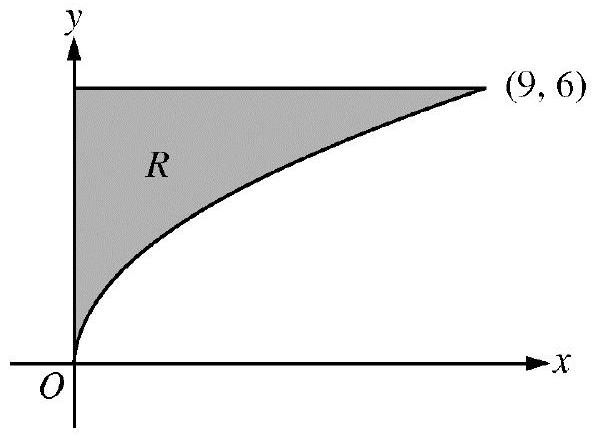
\includegraphics[width=0.6\linewidth]{figures/bc-2010_fig1.jpg}
\end{center}
Let $R$ be the region in the first quadrant bounded by the graph of $y=2 \sqrt{x}$, the horizontal line $y=6$, and the $y$-axis, as shown in the figure above.\\
\begin{parts}
\part Find the area of $R$.
\part Write, but do not evaluate, an integral expression that gives the volume of the solid generated when $R$ is rotated about the horizontal line $y=7$.
\part Region $R$ is the base of a solid. For each $y$, where $0 \leq y \leq 6$, the cross section of the solid taken perpendicular to the $y$-axis is a rectangle whose height is 3 times the length of its base in region $R$. Write, but do not evaluate, an integral expression that gives the volume of the solid.
\end{parts}
\begin{solution}
\begin{parts}
\part Area $=\int_{0}^{9}(6-2 \sqrt{x}) d x=\left.\left(6 x-\frac{4}{3} x^{3 / 2}\right)\right|_{x=0} ^{x=9}=18$
\part Volume $=\pi \int_{0}^{9}\left((7-2 \sqrt{x})^{2}-(7-6)^{2}\right) d x$
\part Solving $y=2 \sqrt{x}$ for $x$ yields $x=\frac{y^{2}}{4}$.

Each rectangular cross section has area $\left(3 \frac{y^{2}}{4}\right)\left(\frac{y^{2}}{4}\right)=\frac{3}{16} y^{4}$.\\
Volume $=\int_{0}^{6} \frac{3}{16} y^{4} d y$
\end{parts}
\par\medskip
\textbf{Rubric:}\par
\begin{parts}
\part $3:\left\{\begin{array}{l}1: \text { integrand } \\ 1: \text { antiderivative } \\ 1: \text { answer }\end{array}\right.$
\part $3:\left\{\begin{array}{l}2: \text { integrand } \\ 1: \text { limits and constant }\end{array}\right.$
\part $3:\left\{\begin{array}{l}2: \text { integrand } \\ 1: \text { answer }\end{array}\right.$
\end{parts}
\end{solution}

\question
% Q5 | 2010 Calculus BC | Part B | Calculator Prohibited
Consider the differential equation $\frac{d y}{d x}=1-y$. Let $y=f(x)$ be the particular solution to this differential equation with the initial condition $f(1)=0$. For this particular solution, $f(x)<1$ for all values of $x$.\\
\begin{parts}
\part Use Euler's method, starting at $x=1$ with two steps of equal size, to approximate $f(0)$. Show the work that leads to your answer.
\part Find $\lim _{x \rightarrow 1} \frac{f(x)}{x^{3}-1}$. Show the work that leads to your answer.
\part Find the particular solution $y=f(x)$ to the differential equation $\frac{d y}{d x}=1-y$ with the initial condition $f(1)=0$.
\end{parts}
\begin{solution}
\begin{parts}
\part $f\left(\frac{1}{2}\right) \approx f(1)+\left(\left.\frac{d y}{d x}\right|_{(1,0)}\right) \cdot \Delta x$

\[\begin{aligned}
& =0+1 \cdot\left(-\frac{1}{2}\right)=-\frac{1}{2} \\
f(0) & \approx f\left(\frac{1}{2}\right)+\left(\left.\frac{d y}{d x}\right|_{\left(\frac{1}{2},-\frac{1}{2}\right)}\right) \cdot \Delta x \\
& \approx-\frac{1}{2}+\frac{3}{2} \cdot\left(-\frac{1}{2}\right)=-\frac{5}{4}
\end{aligned}\]
\part Since $f$ is differentiable at $x=1, f$ is continuous at $x=1$. So, $\lim _{x \rightarrow 1} f(x)=0=\lim _{x \rightarrow 1}\left(x^{3}-1\right)$ and we may apply L'Hospital's Rule.\\
$\lim _{x \rightarrow 1} \frac{f(x)}{x^{3}-1}=\lim _{x \rightarrow 1} \frac{f^{\prime}(x)}{3 x^{2}}=\frac{\lim _{x \rightarrow 1} f^{\prime}(x)}{\lim _{x \rightarrow 1} 3 x^{2}}=\frac{1}{3}$
\part $\frac{d y}{d x}=1-y$

\begin{align*}& \int \frac{1}{1-y} d y=\int 1 d x \\
& -\ln |1-y|=x+C \\
& -\ln 1=1+C \Rightarrow C=-1 \\
& \ln |1-y|=1-x \\
& |1-y|=e^{1-x} \\
& f(x)=1-e^{1-x}\end{align*}
\end{parts}
\par\medskip
\textbf{Rubric:}\par
\begin{parts}
\part $2:\left\{\begin{array}{l}1: \text { Euler's method with two steps } \\ 1: \text { answer }\end{array}\right.$
\part $2:\left\{\begin{array}{l}1: \text { use of L'Hospital's Rule } \\ 1: \text { answer }\end{array}\right.$
\part $5:\left\{\begin{array}{l}1: \text { separation of variables } \\ 1: \text { antiderivatives } \\ 1: \text { constant of integration } \\ 1: \text { uses initial condition } \\ 1: \text { solves for } y\end{array}\right.$
\part Note: $\max 2 / 5$ [1-1-0-0-0] if no constant of integration
\part Note: $0 / 5$ if no separation of variables
\end{parts}
\end{solution}

\question
% Q6 | 2010 Calculus BC | Part B | Calculator Prohibited
\[f(x)= \begin{cases}\frac{\cos x-1}{x^{2}} & \text { for } x \neq 0 \\ -\frac{1}{2} & \text { for } x=0\end{cases}\]
The function $f$, defined above, has derivatives of all orders. Let $g$ be the function defined by $g(x)=1+\int_{0}^{x} f(t) d t$.\\
\begin{parts}
\part Write the first three nonzero terms and the general term of the Taylor series for $\cos x$ about $x=0$. Use this series to write the first three nonzero terms and the general term of the Taylor series for $f$ about $x=0$.
\part Use the Taylor series for $f$ about $x=0$ found in part (a) to determine whether $f$ has a relative maximum, relative minimum, or neither at $x=0$. Give a reason for your answer.
\part Write the fifth-degree Taylor polynomial for $g$ about $x=0$.
\part The Taylor series for $g$ about $x=0$, evaluated at $x=1$, is an alternating series with individual terms that decrease in absolute value to 0 . Use the third-degree Taylor polynomial for $g$ about $x=0$ to estimate the value of $g(1)$. Explain why this estimate differs from the actual value of $g(1)$ by less than $\frac{1}{6!}$.
\end{parts}
\begin{solution}
\begin{parts}
\part $\quad \cos (x)=1-\frac{x^{2}}{2}+\frac{x^{4}}{4!}-\cdots+(-1)^{n} \frac{x^{2 n}}{(2 n)!}+\cdots$

\[f(x)=-\frac{1}{2}+\frac{x^{2}}{4!}-\frac{x^{4}}{6!}+\cdots+(-1)^{n+1} \frac{x^{2 n}}{(2 n+2)!}+\cdots\]
\part $f^{\prime}(0)$ is the coefficient of $x$ in the Taylor series for $f$ about $x=0$, so $f^{\prime}(0)=0$.\\
$\frac{f^{\prime \prime}(0)}{2!}=\frac{1}{4!}$ is the coefficient of $x^{2}$ in the Taylor series for $f$ about $x=0$, so $f^{\prime \prime}(0)=\frac{1}{12}$.\\
Therefore, by the Second Derivative Test, $f$ has a relative minimum at $x=0$.
\part $P_{5}(x)=1-\frac{x}{2}+\frac{x^{3}}{3 \cdot 4!}-\frac{x^{5}}{5 \cdot 6!}$
\part $g(1) \approx 1-\frac{1}{2}+\frac{1}{3 \cdot 4!}=\frac{37}{72}$

Since the Taylor series for $g$ about $x=0$ evaluated at $x=1$ is alternating and the terms decrease in absolute value to 0 , we know $\left|g(1)-\frac{37}{72}\right|<\frac{1}{5 \cdot 6!}<\frac{1}{6!}$.
\end{parts}
\par\medskip
\textbf{Rubric:}\par
\begin{parts}
\part $2:\left\{\begin{array}{l}
1: \text { two correct terms } \\
1: \text { remaining terms }
\end{array}\right.$
\part $2:\left\{\begin{array}{l}
1: \text { estimate } \\
1: \text { explanation }
\end{array}\right.$
\end{parts}
\end{solution}

\end{questions}

\section*{2010 AP Calculus BC Form B}

\begin{questions}

\question
% Q1 | 2010 Calculus BC Form B | Part A | Calculator Active
\begin{center}
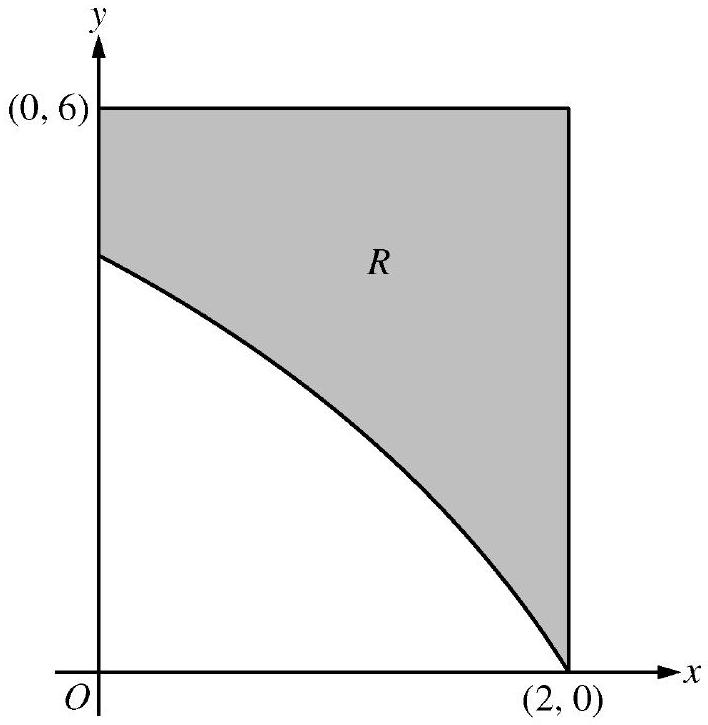
\includegraphics[width=0.6\linewidth]{figures/bc-2010-form-b_fig1.jpg}
\end{center}
In the figure above, $R$ is the shaded region in the first quadrant bounded by the graph of $y=4 \ln (3-x)$, the horizontal line $y=6$, and the vertical line $x=2$.\\
\begin{parts}
\part Find the area of $R$.
\part Find the volume of the solid generated when $R$ is revolved about the horizontal line $y=8$.
\part The region $R$ is the base of a solid. For this solid, each cross section perpendicular to the $x$-axis is a square. Find the volume of the solid.
\end{parts}
\begin{solution}
\begin{parts}
\part $\quad \int_{0}^{2}(6-4 \ln (3-x)) d x=6.816$ or 6.817\\
$2:\left\{\begin{array}{l}1: \text { integrand } \\ 1: \text { answer }\end{array}\right.$
\part $\quad \pi \int_{0}^{2}\left((8-4 \ln (3-x))^{2}-(8-6)^{2}\right) d x$\\
$=168.179$ or 168.180

1 : Correct limits in an integral in (a), (b), or (c)\\
(c)\\
(c)
\part $\quad \int_{0}^{2}(6-4 \ln (3-x))^{2} d x=26.266$ or 26.267\\
$:\left\{\begin{array}{l}1: \text { integrand } \\ 1: \text { answer }\end{array}\right.$
\end{parts}
\par\medskip
\textbf{Rubric:}\par
\begin{parts}
\part $3:\left\{\begin{array}{l}2: \text { integrand } \\ 1: \text { answer }\end{array}\right.$
\part $3:\left\{\begin{array}{l}2: \text { integrand } \\ 1: \text { answer }\end{array}\right.$
\end{parts}
\end{solution}

\question
% Q2 | 2010 Calculus BC Form B | Part A | Calculator Active
The velocity vector of a particle moving in the $x y$-plane has components given by

\[\frac{d x}{d t}=14 \cos \left(t^{2}\right) \sin \left(e^{t}\right) \text { and } \frac{d y}{d t}=1+2 \sin \left(t^{2}\right), \text { for } 0 \leq t \leq 1.5 .\]

At time $t=0$, the position of the particle is $(-2,3)$.\\
\begin{parts}
\part For $0<t<1.5$, find all values of $t$ at which the line tangent to the path of the particle is vertical.
\part Write an equation for the line tangent to the path of the particle at $t=1$.
\part Find the speed of the particle at $t=1$.
\part Find the acceleration vector of the particle at $t=1$.

\begin{center}
\begin{tabular}{|c||c|c|c|c|c|c|c|}
\hline
$t$ & 0 & 2 & 4 & 6 & 8 & 10 & 12 \\
\hline
$P(t)$ & 0 & 46 & 53 & 57 & 60 & 62 & 63 \\
\hline
\end{tabular}
\end{center}
\end{parts}
\begin{solution}
\begin{parts}
\part The tangent line is vertical when $x^{\prime}(t)=0$ and $y^{\prime}(t) \neq 0$. On $0<t<1.5$, this happens at $t=1.253$ and $t=1.144$ or 1.145.
\part $\left.\quad \frac{d y}{d x}\right|_{t=1}=\frac{y^{\prime}(1)}{x^{\prime}(1)}=0.863447$

\begin{align*}& x(1)=-2+\int_{0}^{1} x^{\prime}(t) d t=9.314695 \\
& y(1)=3+\int_{0}^{1} y^{\prime}(t) d t=4.620537\end{align*}

The line tangent to the path of the particle at $t=1$ has equation $y=4.621+0.863(x-9.315)$.
\part Speed $=\sqrt{\left(x^{\prime}(1)\right)^{2}+\left(y^{\prime}(1)\right)^{2}}=4.105$
\part Acceleration vector: $\left\langle x^{\prime \prime}(1), y^{\prime \prime}(1)\right\rangle=\langle-28.425,2.161\rangle$
\end{parts}
\par\medskip
\textbf{Rubric:}\par
\begin{parts}
\part $2:\left\{\begin{array}{l}
1: \text { sets } \frac{d x}{d y}=0 \\
1: \text { answer }
\end{array}\right.$
\part $4:\left\{\begin{array}{l}1:\left.\frac{d y}{d x}\right|_{t=1} \\ 1: x(1) \\ 1: y(1) \\ 1: \text { equation }\end{array}\right.$
\part 1 : answer
\part $2:\left\{\begin{array}{l}1: x^{\prime \prime}(1) \\ 1: y^{\prime \prime}(1)\end{array}\right.$
\end{parts}
\end{solution}

\question
% Q3 | 2010 Calculus BC Form B | Part A | Calculator Active
\begin{center}
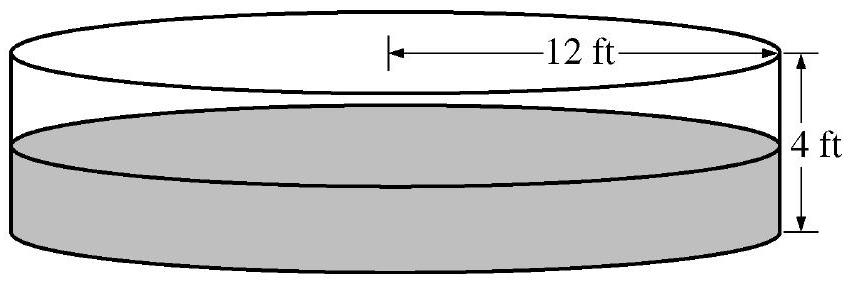
\includegraphics[width=0.6\linewidth]{figures/bc-2010-form-b_fig2.jpg}
\end{center}
The figure above shows an aboveground swimming pool in the shape of a cylinder with a radius of 12 feet and a height of 4 feet. The pool contains 1000 cubic feet of water at time $t=0$. During the time interval $0 \leq t \leq 12$ hours, water is pumped into the pool at the rate $P(t)$ cubic feet per hour. The table above gives values of $P(t)$ for selected values of $t$. During the same time interval, water is leaking from the pool at the rate $R(t)$ cubic feet per hour, where $R(t)=25 e^{-0.05 t}$. (Note: The volume $V$ of a cylinder with radius $r$ and height $h$ is given by $V=\pi r^{2} h$.)\\
\begin{parts}
\part Use a midpoint Riemann sum with three subintervals of equal length to approximate the total amount of water that was pumped into the pool during the time interval $0 \leq t \leq 12$ hours. Show the computations that lead to your answer.
\part Calculate the total amount of water that leaked out of the pool during the time interval $0 \leq t \leq 12$ hours.
\part Use the results from parts (a) and (b) to approximate the volume of water in the pool at time $t=12$ hours. Round your answer to the nearest cubic foot.
\part Find the rate at which the volume of water in the pool is increasing at time $t=8$ hours. How fast is the water level in the pool rising at $t=8$ hours? Indicate units of measure in both answers.
\end{parts}
\begin{solution}
\begin{parts}
\part $\quad \int_{0}^{12} P(t) d t \approx 46 \cdot 4+57 \cdot 4+62 \cdot 4=660 \mathrm{ft}^{3}$
\part $\quad \int_{0}^{12} R(t) d t=225.594 \mathrm{ft}^{3}$
\part $1000+\int_{0}^{12} P(t) d t-\int_{0}^{12} R(t) d t=1434.406$

At time $t=12$ hours, the volume of water in the pool is approximately $1434 \mathrm{ft}^{3}$.
\part $\quad V^{\prime}(t)=P(t)-R(t)$\\
$V^{\prime}(8)=P(8)-R(8)=60-25 e^{-0.4}=43.241$ or $43.242 \mathrm{ft}^{3} / \mathrm{hr}$\\
$V=\pi(12)^{2} h$\\
$\frac{d V}{d t}=144 \pi \frac{d h}{d t}$\\
$\left.\frac{d h}{d t}\right|_{t=8}=\left.\frac{1}{144 \pi} \cdot \frac{d V}{d t}\right|_{t=8}=0.095$ or $0.096 \mathrm{ft} / \mathrm{hr}$
\end{parts}
\par\medskip
\textbf{Rubric:}\par
\begin{parts}
\part $2:\left\{\begin{array}{l}1: \text { midpoint sum } \\ 1: \text { answer }\end{array}\right.$
\part $2:\left\{\begin{array}{l}1: \text { integral } \\ 1: \text { answer }\end{array}\right.$
\part 1 : answer
\part $4:\left\{\begin{array}{l}1: V^{\prime}(8) \\ 1: \text { equation relating } \frac{d V}{d t} \text { and } \frac{d h}{d t} \\ 1:\left.\frac{d h}{d t}\right|_{t=8} \\ 1: \text { units of } \mathrm{ft}^{3} / \mathrm{hr} \text { and } \mathrm{ft} / \mathrm{hr}\end{array}\right.$
\end{parts}
\end{solution}

\question
% Q4 | 2010 Calculus BC Form B | Part B | Calculator Prohibited
\begin{center}
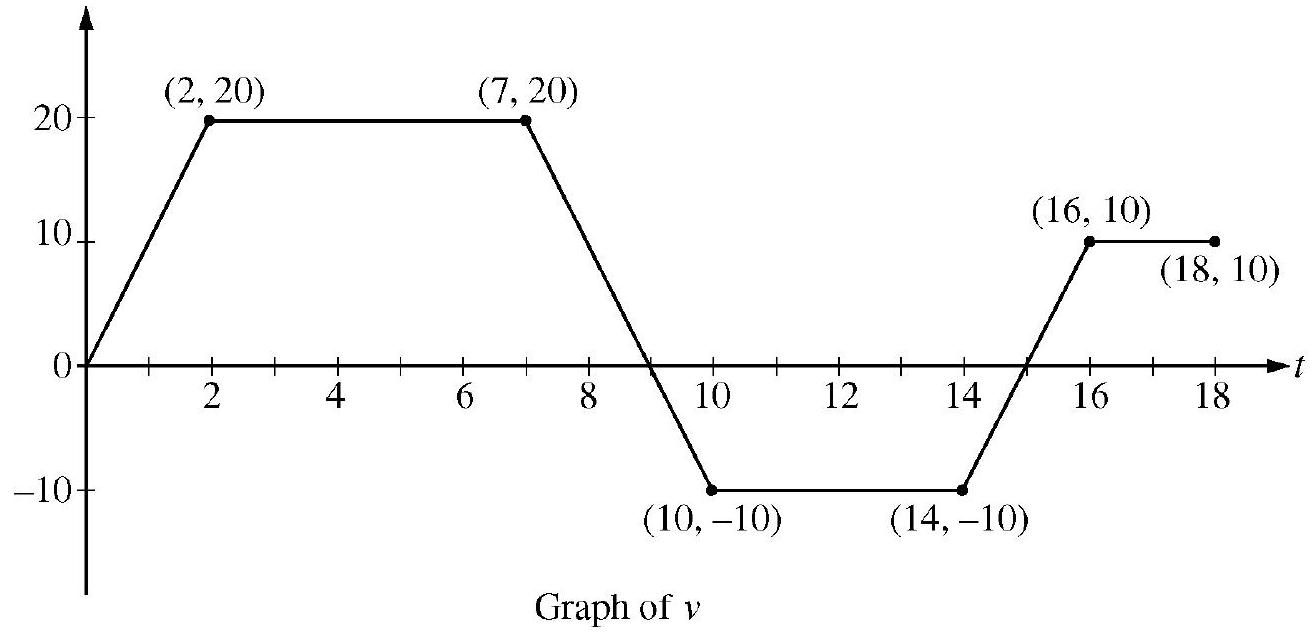
\includegraphics[width=0.6\linewidth]{figures/bc-2010-form-b_fig3.jpg}
\end{center}
A squirrel starts at building $A$ at time $t=0$ and travels along a straight, horizontal wire connected to building $B$. For $0 \leq t \leq 18$, the squirrel's velocity is modeled by the piecewise-linear function defined by the graph above.\\
\begin{parts}
\part At what times in the interval $0<t<18$, if any, does the squirrel change direction? Give a reason for your answer.
\part At what time in the interval $0 \leq t \leq 18$ is the squirrel farthest from building $A$ ? How far from building $A$ is the squirrel at that time?
\part Find the total distance the squirrel travels during the time interval $0 \leq t \leq 18$.
\part Write expressions for the squirrel's acceleration $a(t)$, velocity $v(t)$, and distance $x(t)$ from building $A$ that are valid for the time interval $7<t<10$.
\end{parts}
\begin{solution}
\begin{parts}
\part The squirrel changes direction whenever its velocity changes sign. This occurs at $t=9$ and $t=15$.
\part Velocity is 0 at $t=0, t=9$, and $t=15$.

\begin{center}
\begin{tabular}{c|l}
$t$ & \multicolumn{1}{|c}{position at time $t$} \\
\hline
0 & 0 \\
9 & $\frac{9+5}{2} \cdot 20=140$ \\
15 & $140-\frac{6+4}{2} \cdot 10=90$ \\
18 & $90+\frac{3+2}{2} \cdot 10=115$ \\
\end{tabular}
\end{center}

The squirrel is farthest from building $A$ at time $t=9$; its greatest distance from the building is 140 .
\part The total distance traveled is $\int_{0}^{18}|v(t)| d t=140+50+25=215$.
\part For $7<t<10, a(t)=\frac{20-(-10)}{7-10}=-10$

\[\begin{aligned}
v(t) & =20-10(t-7)=-10 t+90 \\
x(7) & =\frac{7+5}{2} \cdot 20=120 \\
x(t) & =x(7)+\int_{7}^{t}(-10 u+90) d u \\
& =120+\left.\left(-5 u^{2}+90 u\right)\right|_{u=7} ^{u=t} \\
& =-5 t^{2}+90 t-265
\end{aligned}\]
\end{parts}
\par\medskip
\textbf{Rubric:}\par
\begin{parts}
\part 1: t \text {-values }
\part 1 : answer
\part 4: $\left\{\begin{array}{l}1: a(t) \\ 1: v(t) \\ 2: x(t)\end{array}\right.$
\end{parts}
\end{solution}

\question
% Q5 | 2010 Calculus BC Form B | Part B | Calculator Prohibited
Let $f$ and $g$ be the functions defined by $f(x)=\frac{1}{x}$ and $g(x)=\frac{4 x}{1+4 x^{2}}$, for all $x>0$.\\
\begin{parts}
\part Find the absolute maximum value of $g$ on the open interval $(0, \infty)$ if the maximum exists. Find the absolute minimum value of $g$ on the open interval $(0, \infty)$ if the minimum exists. Justify your answers.
\part Find the area of the unbounded region in the first quadrant to the right of the vertical line $x=1$, below the graph of $f$, and above the graph of $g$.
\end{parts}
\begin{solution}
\begin{parts}
\part $g^{\prime}(x)=\frac{4\left(1+4 x^{2}\right)-4 x(8 x)}{\left(1+4 x^{2}\right)^{2}}=\frac{4\left(1-4 x^{2}\right)}{\left(1+4 x^{2}\right)^{2}}$

For $x>0, g^{\prime}(x)=0$ for $x=\frac{1}{2}$.\\
$g^{\prime}(x)>0$ for $0<x<\frac{1}{2}$\\
$g^{\prime}(x)<0$ for $x>\frac{1}{2}$\\
$g\left(\frac{1}{2}\right)=1$\\
Therefore $g$ has a maximum value of 1 at $x=\frac{1}{2}$, and $g$ has no minimum value on the open interval $(0, \infty)$.
\part $\quad \int_{1}^{\infty}(f(x)-g(x)) d x=\lim _{b \rightarrow \infty} \int_{1}^{b}(f(x)-g(x)) d x$\\
$=\left.\lim _{b \rightarrow \infty}\left(\ln (x)-\frac{1}{2} \ln \left(1+4 x^{2}\right)\right)\right|_{x=1} ^{x=b}$\\
$=\lim _{b \rightarrow \infty}\left(\ln (b)-\frac{1}{2} \ln \left(1+4 b^{2}\right)+\frac{1}{2} \ln (5)\right)$\\
$=\lim _{b \rightarrow \infty} \ln \left(\frac{b \sqrt{5}}{\sqrt{1+4 b^{2}}}\right)$\\
$=\lim _{b \rightarrow \infty} \ln \left(\frac{\sqrt{5 b^{2}}}{\sqrt{1+4 b^{2}}}\right)$\\
$=\frac{1}{2} \lim _{b \rightarrow \infty} \ln \left(\frac{5 b^{2}}{1+4 b^{2}}\right)$\\
$=\frac{1}{2} \ln \frac{5}{4}$
\end{parts}
\par\medskip
\textbf{Rubric:}\par
\begin{parts}
\part $5:\left\{\begin{array}{l}
2: g^{\prime}(x) \\
1: \text { critical point } \\
1: \text { answers } \\
1: \text { justification }
\end{array}\right.$
\part $4:\left\{\begin{array}{l}
1: \text { integral } \\
2: \text { antidifferentiation } \\
1: \text { answer }
\end{array}\right.$
\end{parts}
\end{solution}

\question
% Q6 | 2010 Calculus BC Form B | Part B | Calculator Prohibited
The Maclaurin series for the function $f$ is given by $f(x)=\sum_{n=2}^{\infty} \frac{(-1)^{n}(2 x)^{n}}{n-1}$ on its interval of convergence.\\
\begin{parts}
\part Find the interval of convergence for the Maclaurin series of $f$. Justify your answer.
\part Show that $y=f(x)$ is a solution to the differential equation $x y^{\prime}-y=\frac{4 x^{2}}{1+2 x}$ for $|x|<R$, where $R$ is the radius of convergence from part (a).
\end{parts}
\begin{solution}
\begin{parts}
\part $\lim _{n \rightarrow \infty}\left|\frac{\frac{(2 x)^{n+1}}{(n+1)-1}}{\frac{(2 x)^{n}}{n-1}}\right|=\lim _{n \rightarrow \infty}\left|2 x \cdot \frac{n-1}{n}\right|=\lim _{n \rightarrow \infty}\left|2 x \cdot \frac{n-1}{n}\right|=|2 x|$\\
$|2 x|<1$ for $|x|<\frac{1}{2}$\\
Therefore the radius of convergence is $\frac{1}{2}$.\\
When $x=-\frac{1}{2}$, the series is $\sum_{n=2}^{\infty} \frac{(-1)^{n}(-1)^{n}}{n-1}=\sum_{n=2}^{\infty} \frac{1}{n-1}$.\\
This is the harmonic series, which diverges.\\
When $x=\frac{1}{2}$, the series is $\sum_{n=2}^{\infty} \frac{(-1)^{n} 1^{n}}{n-1}=\sum_{n=2}^{\infty} \frac{(-1)^{n}}{n-1}$.\\
This is the alternating harmonic series, which converges.\\
The interval of convergence for the Maclaurin series of $f$ is $\left(-\frac{1}{2}, \frac{1}{2}\right]$.
\part $y=\frac{(2 x)^{2}}{1}-\frac{(2 x)^{3}}{2}+\frac{(2 x)^{4}}{3}-\cdots+\frac{(-1)^{n}(2 x)^{n}}{n-1}+\cdots$

\[=4 x^{2}-4 x^{3}+\frac{16}{3} x^{4}-\cdots+\frac{(-1)^{n}(2 x)^{n}}{n-1}+\cdots\]

$y^{\prime}=8 x-12 x^{2}+\frac{64}{3} x^{3}-\cdots+\frac{(-1)^{n} n(2 x)^{n-1} \cdot 2}{n-1}+\cdots$\\
$x y^{\prime}=8 x^{2}-12 x^{3}+\frac{64}{3} x^{4}-\cdots+\frac{(-1)^{n} n(2 x)^{n}}{n-1}+\cdots$\\
$x y^{\prime}-y=4 x^{2}-8 x^{3}+16 x^{4}-\cdots+(-1)^{n}(2 x)^{n}+\cdots$

\[=4 x^{2}\left(1-2 x+4 x^{2}-\cdots+(-1)^{n}(2 x)^{n-2}+\cdots\right)\]

The series $1-2 x+4 x^{2}-\cdots+(-1)^{n}(2 x)^{n-2}+\cdots=\sum_{n=0}^{\infty}(-2 x)^{n}$ is a geometric series that converges to $\frac{1}{1+2 x}$ for $|x|<\frac{1}{2}$. Therefore $x y^{\prime}-y=4 x^{2} \cdot \frac{1}{1+2 x}$ for $|x|<\frac{1}{2}$.
\end{parts}
\par\medskip
\textbf{Rubric:}\par
\begin{parts}
\part $5:\left\{\begin{array}{l}1: \text { sets up ratio } \\ 1: \text { limit evaluation } \\ 1: \text { radius of convergence } \\ 1: \text { considers both endpoints } \\ 1: \text { analysis and interval of } \\ \quad \text { convergence }\end{array}\right.$
\part $4:\left\{\begin{array}{l}1: \text { series for } y^{\prime} \\ 1: \text { series for } x y^{\prime} \\ 1: \text { series for } x y^{\prime}-y \\ 1: \text { analysis with geometric series }\end{array}\right.$
\end{parts}
\end{solution}

\end{questions}

\section*{2011 AP Calculus BC}

\begin{questions}

\question
% Q1 | 2011 Calculus BC | Part A | Calculator Active
At time $t$, a particle moving in the $x y$-plane is at position $(x(t), y(t))$, where $x(t)$ and $y(t)$ are not explicitly given. For $t \geq 0, \frac{d x}{d t}=4 t+1$ and $\frac{d y}{d t}=\sin \left(t^{2}\right)$. At time $t=0, x(0)=0$ and $y(0)=-4$.\\
\begin{parts}
\part Find the speed of the particle at time $t=3$, and find the acceleration vector of the particle at time $t=3$.
\part Find the slope of the line tangent to the path of the particle at time $t=3$.
\part Find the position of the particle at time $t=3$.
\part Find the total distance traveled by the particle over the time interval $0 \leq t \leq 3$.
\end{parts}
\begin{solution}
\begin{parts}
\part Speed $=\sqrt{\left(x^{\prime}(3)\right)^{2}+\left(y^{\prime}(3)\right)^{2}}=13.006$ or 13.007

\begin{align*}\text { Acceleration } & =\left\langle x^{\prime \prime}(3), y^{\prime \prime}(3)\right\rangle \\
& =\langle 4,-5.466\rangle \text { or }\langle 4,-5.467\rangle\end{align*}
\part Slope $=\frac{y^{\prime}(3)}{x^{\prime}(3)}=0.031$ or 0.032
\part $\quad x(3)=0+\int_{0}^{3} \frac{d x}{d t} d t=21$

\[y(3)=-4+\int_{0}^{3} \frac{d y}{d t} d t=-3.226\]

At time $t=3$, the particle is at position $(21,-3.226)$.
\part Distance $=\int_{0}^{3} \sqrt{\left(\frac{d x}{d t}\right)^{2}+\left(\frac{d y}{d t}\right)^{2}} d t=21.091$
\end{parts}
\par\medskip
\textbf{Rubric:}\par
\begin{parts}
\part $2:\left\{\begin{array}{l}
1: \text { speed } \\
1: \text { acceleration }
\end{array}\right.$
\part 1 : answer
\part $4:\left\{\begin{array}{c}
2: x \text {-coordinate } \\
1: \text { integral } \\
1: \text { answer } \\
2: y \text {-coordinate } \\
1: \text { integral } \\
1: \text { answer }
\end{array}\right.$
\part $2:\left\{\begin{array}{l}
1: \text { integral } \\
1: \text { answer }
\end{array}\right.$
\end{parts}
\end{solution}

\question
% Q2 | 2011 Calculus BC | Part A | Calculator Active
\begin{center}
\begin{tabular}{|c||c|c|c|c|c|}
\hline
\begin{tabular}{c}
$t$ \\
(minutes) \\
\end{tabular} & 0 & 2 & 5 & 9 & 10 \\
\hline
\begin{tabular}{c}
$H(t)$ \\
(degrees Celsius) \\
\end{tabular} & 66 & 60 & 52 & 44 & 43 \\
\hline
\end{tabular}
\end{center}
As a pot of tea cools, the temperature of the tea is modeled by a differentiable function $H$ for $0 \leq t \leq 10$, where time $t$ is measured in minutes and temperature $H(t)$ is measured in degrees Celsius. Values of $H(t)$ at selected values of time $t$ are shown in the table above.\\
\begin{parts}
\part Use the data in the table to approximate the rate at which the temperature of the tea is changing at time $t=3.5$. Show the computations that lead to your answer.
\part Using correct units, explain the meaning of $\frac{1}{10} \int_{0}^{10} H(t) d t$ in the context of this problem. Use a trapezoidal sum with the four subintervals indicated by the table to estimate $\frac{1}{10} \int_{0}^{10} H(t) d t$.
\part Evaluate $\int_{0}^{10} H^{\prime}(t) d t$. Using correct units, explain the meaning of the expression in the context of this problem.
\part At time $t=0$, biscuits with temperature $100^{\circ} \mathrm{C}$ were removed from an oven. The temperature of the biscuits at time $t$ is modeled by a differentiable function $B$ for which it is known that $B^{\prime}(t)=-13.84 e^{-0.173 t}$. Using the given models, at time $t=10$, how much cooler are the biscuits than the tea?
\end{parts}
\begin{solution}
\begin{parts}
\part $H^{\prime}(3.5) \approx \frac{H(5)-H(2)}{5-2}$

\[=\frac{52-60}{3}=-2.666 \text { or }-2.667 \text { degrees Celsius per minute }\]
\part $\frac{1}{10} \int_{0}^{10} H(t) d t$ is the average temperature of the tea, in degrees Celsius, over the 10 minutes.

\[\begin{aligned}
\frac{1}{10} \int_{0}^{10} H(t) d t & \approx \frac{1}{10}\left(2 \cdot \frac{66+60}{2}+3 \cdot \frac{60+52}{2}+4 \cdot \frac{52+44}{2}+1 \cdot \frac{44+43}{2}\right) \\
& =52.95
\end{aligned}\]
\part $\int_{0}^{10} H^{\prime}(t) d t=H(10)-H(0)=43-66=-23$

The temperature of the tea drops 23 degrees Celsius from time $t=0$ to time $t=10$ minutes.
\part $B(10)=100+\int_{0}^{10} B^{\prime}(t) d t=34.18275 ; \quad H(10)-B(10)=8.817$

The biscuits are 8.817 degrees Celsius cooler than the tea.
\end{parts}
\par\medskip
\textbf{Rubric:}\par
\begin{parts}
\part 1 : answer
\part $3:\left\{\begin{array}{l}1: \text { meaning of expression } \\ 1: \text { trapezoidal sum } \\ 1: \text { estimate }\end{array}\right.$
\part $2:\left\{\begin{array}{l}1: \text { value of integral } \\ 1: \text { meaning of expression }\end{array}\right.$
\part $3:\left\{\begin{array}{l}1: \text { integrand } \\ 1: \text { uses } B(0)=100 \\ 1: \text { answer }\end{array}\right.$
\end{parts}
\end{solution}

\question
% Q3 | 2011 Calculus BC | Part B | Calculator Prohibited
\begin{center}
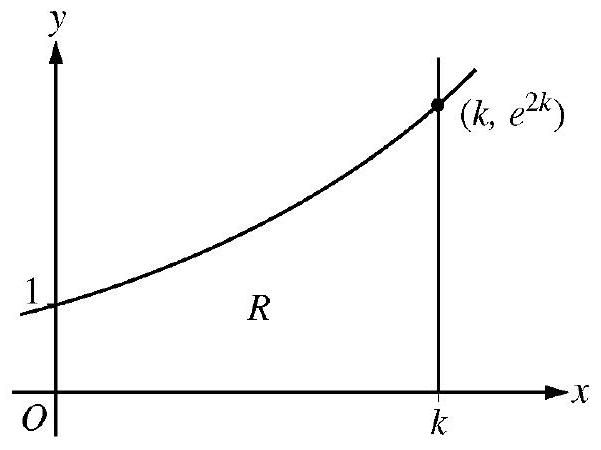
\includegraphics[width=0.6\linewidth]{figures/bc-2011_fig1.jpg}
\end{center}
Let $f(x)=e^{2 x}$. Let $R$ be the region in the first quadrant bounded by the graph of $f$, the coordinate axes, and the vertical line $x=k$, where $k>0$. The region $R$ is shown in the figure above.\\

\begin{center}
  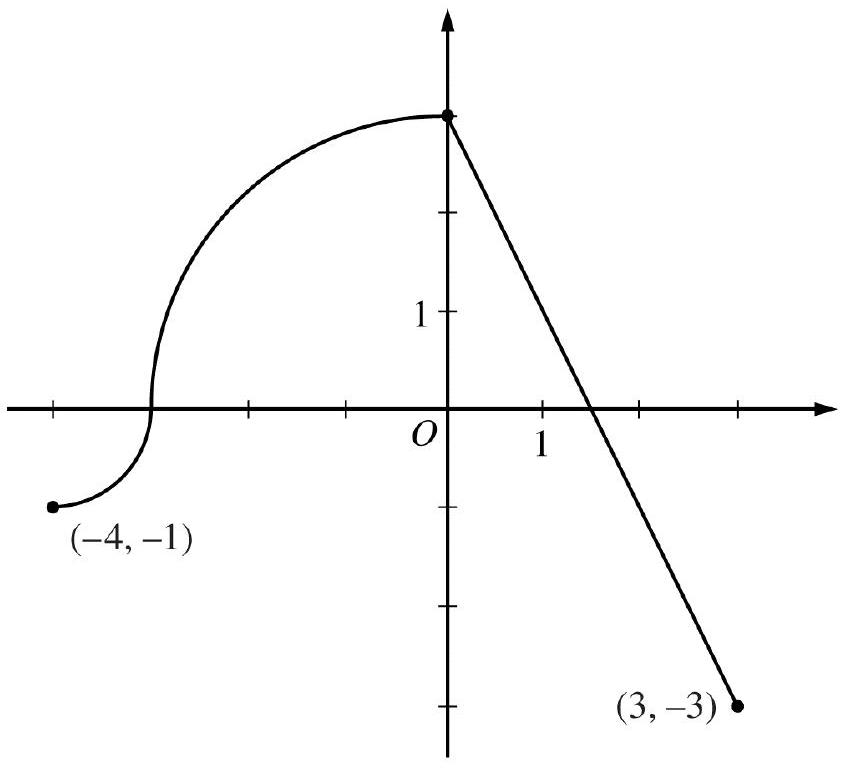
\includegraphics[width=0.6\linewidth]{figures/bc-2011_fig2.jpg}
\end{center}
\begin{parts}
\part Write, but do not evaluate, an expression involving an integral that gives the perimeter of $R$ in terms of $k$.
\part The region $R$ is rotated about the $x$-axis to form a solid. Find the volume, $V$, of the solid in terms of $k$.
\part The volume $V$, found in part (b), changes as $k$ changes. If $\frac{d k}{d t}=\frac{1}{3}$, determine $\frac{d V}{d t}$ when $k=\frac{1}{2}$.
\end{parts}
\begin{solution}
\begin{parts}
\part $f^{\prime}(x)=2 e^{2 x}$

\[\text { Perimeter }=1+k+e^{2 k}+\int_{0}^{k} \sqrt{1+\left(2 e^{2 x}\right)^{2}} d x\]
\part Volume $=\pi \int_{0}^{k}\left(e^{2 x}\right)^{2} d x=\pi \int_{0}^{k} e^{4 x} d x=\left.\frac{\pi}{4} e^{4 x}\right|_{x=0} ^{x=k}=\frac{\pi}{4} e^{4 k}-\frac{\pi}{4}$
\part $\frac{d V}{d t}=\pi e^{4 k} \frac{d k}{d t}$

When $k=\frac{1}{2}, \frac{d V}{d t}=\pi e^{2} \cdot \frac{1}{3}$.
\end{parts}
\par\medskip
\textbf{Rubric:}\par
\begin{parts}
\part $3:\left\{\begin{array}{l}1: f^{\prime}(x) \\ 1: \text { integral } \\ 1: \text { answer }\end{array}\right.$
\part $4:\left\{\begin{array}{l}1: \text { integrand } \\ 1: \text { limits } \\ 1: \text { antiderivative } \\ 1: \text { answer }\end{array}\right.$
\part $2:\left\{\begin{array}{l}1 \text { : applies chain rule } \\ 1 \text { : answer }\end{array}\right.$
\end{parts}
\end{solution}

\question
% Q4 | 2011 Calculus BC | Part B | Calculator Prohibited
The continuous function $f$ is defined on the interval $-4 \leq x \leq 3$. The graph of $f$ consists of two quarter circles and one line segment, as shown in the figure below. Let $g(x)=2 x+\int_{0}^{x} f(t) d t$.\\
\begin{parts}
\part Find $g(-3)$. Find $g^{\prime}(x)$ and evaluate $g^{\prime}(-3)$.
\part Determine the $x$-coordinate of the point at which $g$ has an absolute maximum on the interval $-4 \leq x \leq 3$. Justify your answer.
\part Find all values of $x$ on the interval $-4<x<3$ for which the graph of $g$ has a point of inflection. Give a reason for your answer.
\part Find the average rate of change of $f$ on the interval $-4 \leq x \leq 3$. There is no point $c,-4<c<3$, for which $f^{\prime}(c)$ is equal to that average rate of change. Explain why this statement does not contradict the Mean Value Theorem.
\end{parts}
\begin{solution}
\begin{parts}
\part $g(-3)=2(-3)+\int_{0}^{-3} f(t) d t=-6-\frac{9 \pi}{4}$\\
$g^{\prime}(x)=2+f(x)$\\
$g^{\prime}(-3)=2+f(-3)=2$
\part $g^{\prime}(x)=0$ when $f(x)=-2$. This occurs at $x=\frac{5}{2}$.\\
$g^{\prime}(x)>0$ for $-4<x<\frac{5}{2}$ and $g^{\prime}(x)<0$ for $\frac{5}{2}<x<3$.\\
Therefore $g$ has an absolute maximum at $x=\frac{5}{2}$.
\part $g^{\prime \prime}(x)=f^{\prime}(x)$ changes sign only at $x=0$. Thus the graph of $g$ has a point of inflection at $x=0$.
\part The average rate of change of $f$ on the interval $-4 \leq x \leq 3$ is $\frac{f(3)-f(-4)}{3-(-4)}=-\frac{2}{7}$.\\
To apply the Mean Value Theorem, $f$ must be differentiable at each point in the interval $-4<x<3$. However, $f$ is not differentiable at $x=-3$ and $x=0$.
\end{parts}
\par\medskip
\textbf{Rubric:}\par
\begin{parts}
\part $3:\left\{\begin{array}{l}1: g(-3) \\ 1: g^{\prime}(x) \\ 1: g^{\prime}(-3)\end{array}\right.$
\part $3:\left\{\begin{array}{l}1: \text { considers } g^{\prime}(x)=0 \\ 1: \text { identifies interior candidate } \\ 1: \text { answer with justification }\end{array}\right.$
\part 1 : answer with reason
\part $2:\left\{\begin{array}{l}1: \text { average rate of change } \\ 1: \text { explanation }\end{array}\right.$
\end{parts}
\end{solution}

\question
% Q5 | 2011 Calculus BC | Part B | Calculator Prohibited
At the beginning of 2010, a landfill contained 1400 tons of solid waste. The increasing function $W$ models the total amount of solid waste stored at the landfill. Planners estimate that $W$ will satisfy the differential equation $\frac{d W}{d t}=\frac{1}{25}(W-300)$ for the next 20 years. $W$ is measured in tons, and $t$ is measured in years from the start of 2010.\\
\begin{parts}
\part Use the line tangent to the graph of $W$ at $t=0$ to approximate the amount of solid waste that the landfill contains at the end of the first 3 months of 2010 (time $t=\frac{1}{4}$ ).
\part Find $\frac{d^{2} W}{d t^{2}}$ in terms of $W$. Use $\frac{d^{2} W}{d t^{2}}$ to determine whether your answer in part (a) is an underestimate or an overestimate of the amount of solid waste that the landfill contains at time $t=\frac{1}{4}$.
\part Find the particular solution $W=W(t)$ to the differential equation $\frac{d W}{d t}=\frac{1}{25}(W-300)$ with initial condition $W(0)=1400$.
\end{parts}
\begin{solution}
\begin{parts}
\part $\left.\frac{d W}{d t}\right|_{t=0}=\frac{1}{25}(W(0)-300)=\frac{1}{25}(1400-300)=44$

The tangent line is $y=1400+44 t$.\\
$W\left(\frac{1}{4}\right) \approx 1400+44\left(\frac{1}{4}\right)=1411$ tons
\part $\frac{d^{2} W}{d t^{2}}=\frac{1}{25} \frac{d W}{d t}=\frac{1}{625}(W-300)$ and $W \geq 1400$

Therefore $\frac{d^{2} W}{d t^{2}}>0$ on the interval $0 \leq t \leq \frac{1}{4}$.\\
The answer in part (a) is an underestimate.
\part $\frac{d W}{d t}=\frac{1}{25}(W-300)$\\
$\int \frac{1}{W-300} d W=\int \frac{1}{25} d t$\\
$\ln |W-300|=\frac{1}{25} t+C$\\
$\ln (1400-300)=\frac{1}{25}(0)+C \Rightarrow \ln (1100)=C$\\
$W-300=1100 e^{\frac{1}{25} t}$\\
$W(t)=300+1100 e^{\frac{1}{25} t}, 0 \leq t \leq 20$

2: $\left\{\begin{array}{l}1: \frac{d W}{d t} \text { at } t=0 \\ 1: \text { answer }\end{array}\right.$
\end{parts}
\par\medskip
\textbf{Rubric:}\par
\begin{parts}
\part $2:\left\{\begin{array}{l}1: \frac{d^{2} W}{d t^{2}} \\ 1: \text { answer with reason }\end{array}\right.$
\part $5:\left\{\begin{array}{l}1: \text { separation of variables } \\ 1: \text { antiderivatives } \\ 1: \text { constant of integration } \\ 1: \text { uses initial condition } \\ 1: \text { solves for } W\end{array}\right.$
\part Note: $\max 2 / 5[1-1-0-0-0]$ if no constant of integration
\part Note: $0 / 5$ if no separation of variables
\end{parts}
\end{solution}

\question
% Q6 | 2011 Calculus BC | Part B | Calculator Prohibited
\begin{center}
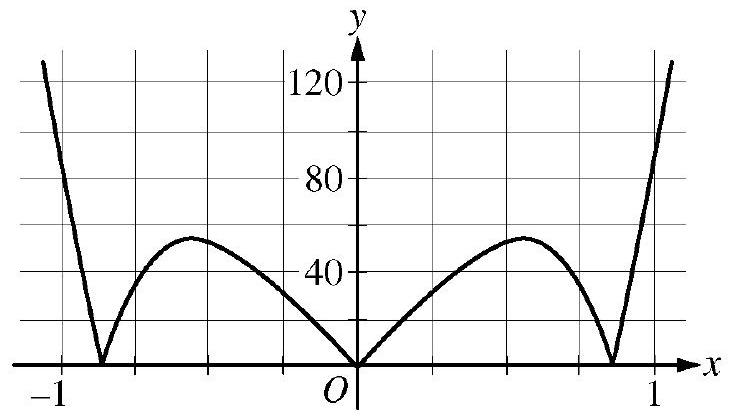
\includegraphics[width=0.6\linewidth]{figures/bc-2011_fig3.jpg}
\end{center}

Graph of $y=\left|f^{(5)}(x)\right|$\\
Let $f(x)=\sin \left(x^{2}\right)+\cos x$. The graph of $y=\left|f^{(5)}(x)\right|$ is shown above.\\
\begin{parts}
\part Write the first four nonzero terms of the Taylor series for $\sin x$ about $x=0$, and write the first four nonzero terms of the Taylor series for $\sin \left(x^{2}\right)$ about $x=0$.
\part Write the first four nonzero terms of the Taylor series for $\cos x$ about $x=0$. Use this series and the series for $\sin \left(x^{2}\right)$, found in part (a), to write the first four nonzero terms of the Taylor series for $f$ about $x=0$.
\part Find the value of $f^{(6)}(0)$.
\part Let $P_{4}(x)$ be the fourth-degree Taylor polynomial for $f$ about $x=0$. Using information from the graph of $y=\left|f^{(5)}(x)\right|$ shown above, show that $\left|P_{4}\left(\frac{1}{4}\right)-f\left(\frac{1}{4}\right)\right|<\frac{1}{3000}$.
\end{parts}
\begin{solution}
\begin{parts}
\part $\quad \sin x=x-\frac{x^{3}}{3!}+\frac{x^{5}}{5!}-\frac{x^{7}}{7!}+\cdots$\\
$\sin \left(x^{2}\right)=x^{2}-\frac{x^{6}}{3!}+\frac{x^{10}}{5!}-\frac{x^{14}}{7!}+\cdots$
\part $\cos x=1-\frac{x^{2}}{2!}+\frac{x^{4}}{4!}-\frac{x^{6}}{6!}+\cdots$\\
$f(x)=1+\frac{x^{2}}{2}+\frac{x^{4}}{4!}-\frac{121 x^{6}}{6!}+\cdots$
\part $\frac{f^{(6)}(0)}{6!}$ is the coefficient of $x^{6}$ in the Taylor series for $f$ about $x=0$. Therefore $f^{(6)}(0)=-121$.
\part The graph of $y=\left|f^{(5)}(x)\right|$ indicates that $\max _{0 \leq x \leq \frac{1}{4}}\left|f^{(5)}(x)\right|<40$.

Therefore\\
$\left|P_{4}\left(\frac{1}{4}\right)-f\left(\frac{1}{4}\right)\right| \leq \frac{\max _{0 \leq x \leq \frac{1}{4}}\left|f^{(5)}(x)\right|}{5!} \cdot\left(\frac{1}{4}\right)^{5}<\frac{40}{120 \cdot 4^{5}}=\frac{1}{3072}<\frac{1}{3000}$.
\end{parts}
\par\medskip
\textbf{Rubric:}\par
\begin{parts}
\part $3:\left\{\begin{array}{l}1: \text { series for } \sin x \\ 2: \text { series for } \sin \left(x^{2}\right)\end{array}\right.$
\part $3:\left\{\begin{array}{l}1: \text { series for } \cos x \\ 2: \text { series for } f(x)\end{array}\right.$
\part 1 : answer
\part $2:\left\{\begin{array}{l}1: \text { form of the error bound } \\ 1: \text { analysis }\end{array}\right.$
\end{parts}
\end{solution}

\end{questions}

\section*{2011 AP Calculus BC Form B}

\begin{questions}

\question
% Q1 | 2011 Calculus BC Form B | Part A | Calculator Active
A cylindrical can of radius 10 millimeters is used to measure rainfall in Stormville. The can is initially empty, and rain enters the can during a 60-day period. The height of water in the can is modeled by the function $S$, where $S(t)$ is measured in millimeters and $t$ is measured in days for $0 \leq t \leq 60$. The rate at which the height of the water is rising in the can is given by $S^{\prime}(t)=2 \sin (0.03 t)+1.5$.\\
\begin{parts}
\part According to the model, what is the height of the water in the can at the end of the 60-day period?
\part According to the model, what is the average rate of change in the height of water in the can over the 60-day period? Show the computations that lead to your answer. Indicate units of measure.
\part Assuming no evaporation occurs, at what rate is the volume of water in the can changing at time $t=7$ ? Indicate units of measure.
\part During the same 60-day period, rain on Monsoon Mountain accumulates in a can identical to the one in Stormville. The height of the water in the can on Monsoon Mountain is modeled by the function $M$, where $M(t)=\frac{1}{400}\left(3 t^{3}-30 t^{2}+330 t\right)$. The height $M(t)$ is measured in millimeters, and $t$ is measured in days for $0 \leq t \leq 60$. Let $D(t)=M^{\prime}(t)-S^{\prime}(t)$. Apply the Intermediate Value Theorem to the function $D$ on the interval $0 \leq t \leq 60$ to justify that there exists a time $t, 0<t<60$, at which the heights of water in the two cans are changing at the same rate.
\end{parts}
\begin{solution}
\begin{parts}
\part $S(60)=\int_{0}^{60} S^{\prime}(t) d t=171.813 \mathrm{~mm}$
\part $\frac{S(60)-S(0)}{60}=2.863$ or $2.864 \mathrm{~mm} /$ day
\part $V(t)=100 \pi S(t) V^{\prime}(7)=100 \pi S^{\prime}(7)=602.218$

The volume of water in the can is increasing at a rate of $602.218 \mathrm{~mm}^{3} /$ day.
\part $D(0)=-0.675<0$ and $D(60)=69.37730>0$

Because $D$ is continuous, the Intermediate Value Theorem implies that there is a time $t, 0<t<60$, at which $D(t)=0$. At this time, the heights of water in the two cans are changing at the same rate.
\end{parts}
\par\medskip
\textbf{Rubric:}\par
\begin{parts}
\part $3:\left\{\begin{array}{l}
1: \text { limits } \\
1: \text { integrand } \\
1: \text { answer }
\end{array}\right.$
\part 1 : answer
\part $2:\left\{\begin{array}{l}
1: \text { relationship between } V \text { and } S \\
1: \text { answer }
\end{array}\right.$
\part $2:\left\{\begin{array}{l}
1: \text { considers } D(0) \text { and } D(60) \\
1: \text { justification }
\end{array}\right.$
\part 1 : units in (b) or (c)
\end{parts}
\end{solution}

\question
% Q2 | 2011 Calculus BC Form B | Part A | Calculator Active
The polar curve $r$ is given by $r(\theta)=3 \theta+\sin \theta$, where $0 \leq \theta \leq 2 \pi$.\\
\begin{parts}
\part Find the area in the second quadrant enclosed by the coordinate axes and the graph of $r$.
\part For $\frac{\pi}{2} \leq \theta \leq \pi$, there is one point $P$ on the polar curve $r$ with $x$-coordinate -3 . Find the angle $\theta$ that corresponds to point $P$. Find the $y$-coordinate of point $P$. Show the work that leads to your answers.
\part A particle is traveling along the polar curve $r$ so that its position at time $t$ is $(x(t), y(t))$ and such that $\frac{d \theta}{d t}=2$. Find $\frac{d y}{d t}$ at the instant that $\theta=\frac{2 \pi}{3}$, and interpret the meaning of your answer in the context of the problem.
\end{parts}
\begin{solution}
\begin{parts}
\part Area $=\frac{1}{2} \int_{\pi / 2}^{\pi}(r(\theta))^{2} d \theta=47.513$
\part $-3=r(\theta) \cos \theta=(3 \theta+\sin \theta) \cos \theta$\\
$\theta=2.01692$\\
$y=r(\theta) \sin (\theta)=6.272$
\part $y=r(\theta) \sin \theta=(3 \theta+\sin \theta) \sin \theta$\\
$\left.\frac{d y}{d t}\right|_{\theta=2 \pi / 3}=\left[\frac{d y}{d \theta} \cdot \frac{d \theta}{d t}\right]_{\theta=2 \pi / 3}=-2.819$\\
The $y$-coordinate of the particle is decreasing at a rate of 2.819 .
\end{parts}
\par\medskip
\textbf{Rubric:}\par
\begin{parts}
\part $3:\left\{\begin{array}{l}1: \text { integrand } \\ 1: \text { limits and constant } \\ 1: \text { answer }\end{array}\right.$
\part $3:\left\{\begin{array}{l}1: \text { equation } \\ 1: \text { value of } \theta \\ 1: y \text {-coordinate }\end{array}\right.$
\part $3:\left\{\begin{array}{l}1: \text { uses chain rule } \\ 1: \text { answer } \\ 1: \text { interpretation }\end{array}\right.$
\end{parts}
\end{solution}

\question
% Q3 | 2011 Calculus BC Form B | Part B | Calculator Prohibited
\begin{center}
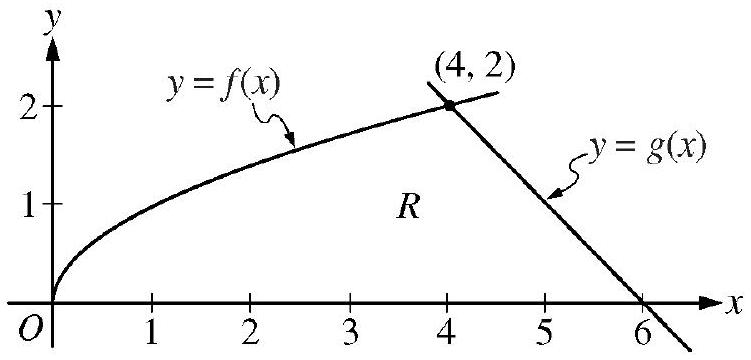
\includegraphics[width=0.6\linewidth]{figures/bc-2011-form-b_fig1.jpg}
\end{center}
The functions $f$ and $g$ are given by $f(x)=\sqrt{x}$ and $g(x)=6-x$. Let $R$ be the region bounded by the $x$-axis and the graphs of $f$ and $g$, as shown in the figure above.\\

\begin{center}
  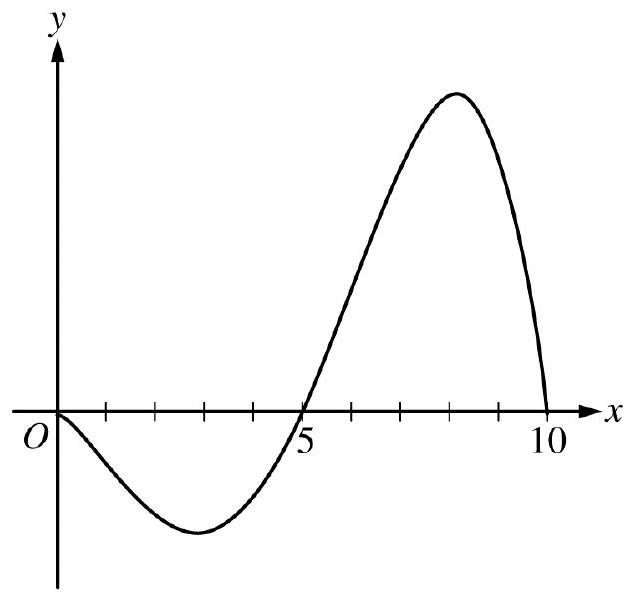
\includegraphics[width=0.6\linewidth]{figures/bc-2011-form-b_fig2.jpg}
\end{center}
\begin{parts}
\part Find the area of $R$.
\part The region $R$ is the base of a solid. For each $y$, where $0 \leq y \leq 2$, the cross section of the solid taken perpendicular to the $y$-axis is a rectangle whose base lies in $R$ and whose height is $2 y$. Write, but do not evaluate, an integral expression that gives the volume of the solid.
\part There is a point $P$ on the graph of $f$ at which the line tangent to the graph of $f$ is perpendicular to the graph of $g$. Find the coordinates of point $P$.
\end{parts}
\begin{solution}
\begin{parts}
\part Area $=\int_{0}^{4} \sqrt{x} d x+\frac{1}{2} \cdot 2 \cdot 2=\left.\frac{2}{3} x^{3 / 2}\right|_{x=0} ^{x=4}+2=\frac{22}{3}$
\part $y=\sqrt{x} \Rightarrow x=y^{2}$\\
$y=6-x \Rightarrow x=6-y$\\
Width $=(6-y)-y^{2}$

Volume $=\int_{0}^{2} 2 y\left(6-y-y^{2}\right) d y$
\part $\quad g^{\prime}(x)=-1$

Thus a line perpendicular to the graph of $g$ has slope 1 .

$f^{\prime}(x)=\frac{1}{2\sqrt{x}}=1 \Rightarrow \sqrt{x}=\frac{1}{2} \Rightarrow x=\frac{1}{4}$

$f\!\left(\frac{1}{4}\right)=\sqrt{\frac{1}{4}}=\frac{1}{2}$

The coordinates of point $P$ are $\left(\frac{1}{4}, \frac{1}{2}\right)$.
\end{parts}
\par\medskip
\textbf{Rubric:}\par
\begin{parts}
\part $3:\left\{\begin{array}{l}
1: \text { integral } \\
1: \text { antiderivative } \\
1: \text { answer }
\end{array}\right.$
\part $3:\left\{\begin{array}{l}2: \text { integrand } \\ 1: \text { answer }\end{array}\right.$
\part $3:\left\{\begin{array}{l}1: f^{\prime}(x) \\ 1: \text { equation } \\ 1: \text { answer }\end{array}\right.$
\end{parts}
\end{solution}

\question
% Q4 | 2011 Calculus BC Form B | Part B | Calculator Prohibited
The graph of the differentiable function $y=f(x)$ with domain $0 \leq x \leq 10$ is shown in the figure below. The area of the region enclosed between the graph of $f$ and the $x$-axis for $0 \leq x \leq 5$ is 10 , and the area of the region enclosed between the graph of $f$ and the $x$-axis for $5 \leq x \leq 10$ is 27 . The arc length for the portion of the graph of $f$ between $x=0$ and $x=5$ is 11, and the arc length for the portion of the graph of $f$ between $x=5$ and $x=10$ is 18 . The function $f$ has exactly two critical points that are located at $x=3$ and $x=8$.\\
\begin{parts}
\part Find the average value of $f$ on the interval $0 \leq x \leq 5$.
\part Evaluate $\int_{0}^{10}(3 f(x)+2) d x$. Show the computations that lead to your answer.
\part Let $g(x)=\int_{5}^{x} f(t) d t$. On what intervals, if any, is the graph of $g$ both concave up and decreasing? Explain your reasoning.
\part The function $h$ is defined by $h(x)=2 f\left(\frac{x}{2}\right)$. The derivative of $h$ is $h^{\prime}(x)=f^{\prime}\left(\frac{x}{2}\right)$. Find the arc length of the graph of $y=h(x)$ from $x=0$ to $x=20$.
\end{parts}
\begin{solution}
\begin{parts}
\part Average value $=\frac{1}{5} \int_{0}^{5} f(x) d x=\frac{-10}{5}=-2$

1 : answer
\part $\int_{0}^{10}(3 f(x)+2) d x=3\left(\int_{0}^{5} f(x) d x+\int_{5}^{10} f(x) d x\right)+20$

2 : answer

\[=3(-10+27)+20=71\]
\part $g^{\prime}(x)=f(x)$\\
$g^{\prime}(x)<0$ on $0<x<5$\\
$g^{\prime}(x)$ is increasing on $3<x<8$.\\
The graph of $g$ is concave up and decreasing on $3<x<5$.
\part Arc length $=\int_{0}^{20} \sqrt{1+\left(h^{\prime}(x)\right)^{2}} d x=\int_{0}^{20} \sqrt{1+\left(f^{\prime}\left(\frac{x}{2}\right)\right)^{2}} d x$

Let $u=\frac{x}{2}$. Then $d u=\frac{1}{2} d x$ and

\[\int_{0}^{20} \sqrt{1+\left(f^{\prime}\left(\frac{x}{2}\right)\right)^{2}} d x=2 \int_{0}^{10} \sqrt{1+\left(f^{\prime}(u)\right)^{2}} d u=2(11+18)=58\]
\end{parts}
\par\medskip
\textbf{Rubric:}\par
\begin{parts}
\part $3:\left\{\begin{array}{l}1: \text { integral } \\ 1: \text { substitution } \\ 1: \text { answer }\end{array}\right.$
\end{parts}
\end{solution}

\question
% Q5 | 2011 Calculus BC Form B | Part B | Calculator Prohibited
\begin{center}
\begin{tabular}{|c|c|c|c|c|}
\hline
\begin{tabular}{c}
$t$ \\
(seconds) \\
\end{tabular} & 0 & 10 & 40 & 60 \\
\hline
\begin{tabular}{c}
$B(t)$ \\
(meters) \\
\end{tabular} & 100 & 136 & 9 & 49 \\
\hline
\begin{tabular}{c}
$v(t)$ \\
(meters per second) \\
\end{tabular} & 2.0 & 2.3 & 2.5 & 4.6 \\
\hline
\end{tabular}
\end{center}
Ben rides a unicycle back and forth along a straight east-west track. The twice-differentiable function $B$ models Ben's position on the track, measured in meters from the western end of the track, at time $t$, measured in seconds from the start of the ride. The table above gives values for $B(t)$ and Ben's velocity, $v(t)$, measured in meters per second, at selected times $t$.\\
\begin{parts}
\part Use the data in the table to approximate Ben's acceleration at time $t=5$ seconds. Indicate units of measure.
\part Using correct units, interpret the meaning of $\int_{0}^{60}|v(t)| d t$ in the context of this problem. Approximate $\int_{0}^{60}|v(t)| d t$ using a left Riemann sum with the subintervals indicated by the data in the table.
\part For $40 \leq t \leq 60$, must there be a time $t$ when Ben's velocity is 2 meters per second? Justify your answer.
\part A light is directly above the western end of the track. Ben rides so that at time $t$, the distance $L(t)$ between Ben and the light satisfies $(L(t))^{2}=12^{2}+(B(t))^{2}$. At what rate is the distance between Ben and the light changing at time $t=40$ ?
\end{parts}
\begin{solution}
\begin{parts}
\part $\quad a(5) \approx \frac{v(10)-v(0)}{10-0}=\frac{0.3}{10}=0.03$ meters $/ \mathrm{sec}^{2}$
\part $\quad \int_{0}^{60}|v(t)| d t$ is the total distance, in meters, Ben rides over the 60 -second interval $t=0$ to $t=60$.

\[\int_{0}^{60}|v(t)| d t \approx 2.0 \cdot 10+2.3(40-10)+2.5(60-40)=139 \text { meters }\]
\part Because $\frac{B(60)-B(40)}{60-40}=\frac{49-9}{20}=2$, the Mean Value Theorem implies there is a time $t, 40<t<60$, such that $v(t)=2$.
\part $2 L(t) L^{\prime}(t)=2 B(t) B^{\prime}(t)$

\[L^{\prime}(40)=\frac{B(40) v(40)}{L(40)}=\frac{9 \cdot 2.5}{\sqrt{144+81}}=\frac{3}{2} \text { meters } / \mathrm{sec}\]
\end{parts}
\par\medskip
\textbf{Rubric:}\par
\begin{parts}
\part 1 : answer
\part $2:\left\{\begin{array}{l}1: \text { meaning of integral } \\ 1: \text { approximation }\end{array}\right.$
\part $2:\left\{\begin{array}{l}1: \text { difference quotient } \\ 1: \text { conclusion with justification }\end{array}\right.$
\part $3:\left\{\begin{array}{l}1: \text { derivatives } \\ 1: \text { uses } B^{\prime}(t)=v(t) \\ 1: \text { answer }\end{array}\right.$
\part 1 : units in (a) or (b)
\end{parts}
\end{solution}

\question
% Q6 | 2011 Calculus BC Form B | Part B | Calculator Prohibited
Let $f(x)=\ln \left(1+x^{3}\right)$.\\
\begin{parts}
\part The Maclaurin series for $\ln (1+x)$ is $x-\frac{x^{2}}{2}+\frac{x^{3}}{3}-\frac{x^{4}}{4}+\cdots+(-1)^{n+1} \cdot \frac{x^{n}}{n}+\cdots$. Use the series to write the first four nonzero terms and the general term of the Maclaurin series for $f$.
\part The radius of convergence of the Maclaurin series for $f$ is 1 . Determine the interval of convergence. Show the work that leads to your answer.
\part Write the first four nonzero terms of the Maclaurin series for $f^{\prime}\left(t^{2}\right)$. If $g(x)=\int_{0}^{x} f^{\prime}\left(t^{2}\right) d t$, use the first two nonzero terms of the Maclaurin series for $g$ to approximate $g(1)$.
\part The Maclaurin series for $g$, evaluated at $x=1$, is a convergent alternating series with individual terms that decrease in absolute value to 0 . Show that your approximation in part (c) must differ from $g(1)$ by less than $\frac{1}{5}$.
\end{parts}
\begin{solution}
\begin{parts}
\part $x^{3}-\frac{x^{6}}{2}+\frac{x^{9}}{3}-\frac{x^{12}}{4}+\cdots+(-1)^{n+1} \cdot \frac{x^{3 n}}{n}+\cdots$
\part The interval of convergence is centered at $x=0$.

At $x=-1$, the series is $-1-\frac{1}{2}-\frac{1}{3}-\frac{1}{4}-\cdots-\frac{1}{n}-\cdots$, which diverges because the harmonic series diverges.\\
At $x=1$, the series is $1-\frac{1}{2}+\frac{1}{3}-\frac{1}{4}+\cdots+(-1)^{n+1} \cdot \frac{1}{n}+\cdots$, the alternating harmonic series, which converges.

Therefore the interval of convergence is $-1<x \leq 1$.
\part The Maclaurin series for $f^{\prime}(x), f^{\prime}\left(t^{2}\right)$, and $g(x)$ are

\[\begin{aligned}
& f^{\prime}(x): \sum_{n=1}^{\infty}(-1)^{n+1} \cdot 3 x^{3 n-1}=3 x^{2}-3 x^{5}+3 x^{8}-3 x^{11}+\cdots \\
& f^{\prime}\left(t^{2}\right): \sum_{n=1}^{\infty}(-1)^{n+1} \cdot 3 t^{6 n-2}=3 t^{4}-3 t^{10}+3 t^{16}-3 t^{22}+\cdots \\
& g(x): \sum_{n=1}^{\infty}(-1)^{n+1} \cdot \frac{3 x^{6 n-1}}{6 n-1}=\frac{3 x^{5}}{5}-\frac{3 x^{11}}{11}+\frac{3 x^{17}}{17}-\frac{3 x^{23}}{23}+\cdots
\end{aligned}\]

Thus $g(1) \approx \frac{3}{5}-\frac{3}{11}=\frac{18}{55}$.
\part The Maclaurin series for $g$ evaluated at $x=1$ is alternating, and the terms decrease in absolute value to 0 .\\
Thus $\left|g(1)-\frac{18}{55}\right|<\frac{3 \cdot 1^{17}}{17}=\frac{3}{17}<\frac{1}{5}$.
\end{parts}
\par\medskip
\textbf{Rubric:}\par
\begin{parts}
\part $2:\left\{\begin{array}{l}1: \text { first four terms } \\ 1: \text { general term }\end{array}\right.$
\part 2 : answer with analysis
\part $4:\left\{\begin{array}{l}1: \text { two terms for } f^{\prime}\left(t^{2}\right) \\ 1: \text { other terms for } f^{\prime}\left(t^{2}\right) \\ 1: \text { first two terms for } g(x) \\ 1: \text { approximation }\end{array}\right.$
\part 1 : analysis
\end{parts}
\end{solution}

\end{questions}

\section*{2012 AP Calculus BC}

\begin{questions}

\question
% Q1 | 2012 Calculus BC | Part A | Calculator Active
\begin{center}
\begin{tabular}{|c||c|c|c|c|c|}
\hline
$t$ (minutes) & 0 & 4 & 9 & 15 & 20 \\
\hline
$W(t)$ (degrees Fahrenheit) & 55.0 & 57.1 & 61.8 & 67.9 & 71.0 \\
\hline
\end{tabular}
\end{center}
The temperature of water in a tub at time $t$ is modeled by a strictly increasing, twice-differentiable function $W$, where $W(t)$ is measured in degrees Fahrenheit and $t$ is measured in minutes. At time $t=0$, the temperature of the water is $55^{\circ} \mathrm{F}$. The water is heated for 30 minutes, beginning at time $t=0$. Values of $W(t)$ at selected times $t$ for the first 20 minutes are given in the table above.\\
\begin{parts}
\part Use the data in the table to estimate $W^{\prime}(12)$. Show the computations that lead to your answer. Using correct units, interpret the meaning of your answer in the context of this problem.
\part Use the data in the table to evaluate $\int_{0}^{20} W^{\prime}(t) d t$. Using correct units, interpret the meaning of $\int_{0}^{20} W^{\prime}(t) d t$ in the context of this problem.
\part For $0 \leq t \leq 20$, the average temperature of the water in the tub is $\frac{1}{20} \int_{0}^{20} W(t) d t$. Use a left Riemann sum with the four subintervals indicated by the data in the table to approximate $\frac{1}{20} \int_{0}^{20} W(t) d t$. Does this approximation overestimate or underestimate the average temperature of the water over these 20 minutes? Explain your reasoning.
\part For $20 \leq t \leq 25$, the function $W$ that models the water temperature has first derivative given by $W^{\prime}(t)=0.4 \sqrt{t} \cos (0.06 t)$. Based on the model, what is the temperature of the water at time $t=25$ ?
\end{parts}
\begin{solution}
\begin{parts}
\part $\quad W^{\prime}(12) \approx \frac{W(15)-W(9)}{15-9}=\frac{67.9-61.8}{6}$

\[=1.017(\text { or } 1.016)\]

The water temperature is increasing at a rate of approximately $1.017^{\circ} \mathrm{F}$ per minute at time $t=12$ minutes.
\part $\int_{0}^{20} W^{\prime}(t) d t=W(20)-W(0)=71.0-55.0=16$

The water has warmed by $16^{\circ} \mathrm{F}$ over the interval from $t=0$ to $t=20$ minutes.
\part $\frac{1}{20} \int_{0}^{20} W(t) d t \approx \frac{1}{20}(4 \cdot W(0)+5 \cdot W(4)+6 \cdot W(9)+5 \cdot W(15))$

\begin{align*}& =\frac{1}{20}(4 \cdot 55.0+5 \cdot 57.1+6 \cdot 61.8+5 \cdot 67.9) \\
& =\frac{1}{20} \cdot 1215.8=60.79\end{align*}

This approximation is an underestimate, because a left Riemann sum is used and the function $W$ is strictly increasing.
\part $W(25)=71.0+\int_{20}^{25} W^{\prime}(t) d t$

\[=71.0+2.043155=73.043\]
\end{parts}
\par\medskip
\textbf{Rubric:}\par
\begin{parts}
\part $2:\left\{\begin{array}{l}
1: \text { estimate } \\
1: \text { interpretation with units }
\end{array}\right.$
\part $2:\left\{\begin{array}{l}
1: \text { value } \\
1: \text { interpretation with units }
\end{array}\right.$
\part $3:\left\{\begin{array}{l}
1: \text { left Riemann sum } \\
1: \text { approximation } \\
1: \text { underestimate with reason }
\end{array}\right.$
\part $2:\left\{\begin{array}{l}
1: \text { integral } \\
1: \text { answer }
\end{array}\right.$
\end{parts}
\end{solution}

\question
% Q2 | 2012 Calculus BC | Part A | Calculator Active
For $t \geq 0$, a particle is moving along a curve so that its position at time $t$ is $(x(t), y(t))$. At time $t=2$, the particle is at position $(1,5)$. It is known that $\frac{d x}{d t}=\frac{\sqrt{t+2}}{e^{t}}$ and $\frac{d y}{d t}=\sin ^{2} t$.\\
\begin{parts}
\part Is the horizontal movement of the particle to the left or to the right at time $t=2$ ? Explain your answer. Find the slope of the path of the particle at time $t=2$.
\part Find the $x$-coordinate of the particle's position at time $t=4$.
\part Find the speed of the particle at time $t=4$. Find the acceleration vector of the particle at time $t=4$.
\part Find the distance traveled by the particle from time $t=2$ to $t=4$.
\end{parts}
\begin{solution}
\begin{parts}
\part $\left.\frac{d x}{d t}\right|_{t=2}=\frac{2}{e^{2}}$

Because $\left.\frac{d x}{d t}\right|_{t=2}>0$, the particle is moving to the right at time $t=2$.

\[\left.\frac{d y}{d x}\right|_{t=2}=\frac{d y /\left.d t\right|_{t=2}}{d x /\left.d t\right|_{t=2}}=3.055(\text { or } 3.054)\]
\part $x(4)=1+\int_{2}^{4} \frac{\sqrt{t+2}}{e^{t}} d t=1.253$ (or 1.252)
\part Speed $=\sqrt{\left(x^{\prime}(4)\right)^{2}+\left(y^{\prime}(4)\right)^{2}}=0.575$ (or 0.574)

\begin{align*}\text { Acceleration } & =\left\langle x^{\prime \prime}(4), y^{\prime \prime}(4)\right\rangle \\
& =\langle-0.041,0.989\rangle\end{align*}
\part Distance $=\int_{2}^{4} \sqrt{\left(x^{\prime}(t)\right)^{2}+\left(y^{\prime}(t)\right)^{2}} d t$

\[=0.651(\text { or } 0.650)\]
\end{parts}
\par\medskip
\textbf{Rubric:}\par
\begin{parts}
\part $3:\left\{\begin{array}{l}1: \text { moving to the right with reason } \\ 1: \text { considers } \frac{d y / d t}{d x / d t} \\ 1: \text { slope at } t=2\end{array}\right.$
\part $2:\left\{\begin{array}{l}1: \text { integral } \\ 1: \text { answer }\end{array}\right.$
\part $2:\left\{\begin{array}{l}1: \text { speed } \\ 1: \text { acceleration }\end{array}\right.$
\part $2:\left\{\begin{array}{l}1: \text { integral } \\ 1: \text { answer }\end{array}\right.$
\end{parts}
\end{solution}

\question
% Q3 | 2012 Calculus BC | Part B | Calculator Prohibited
\begin{center}
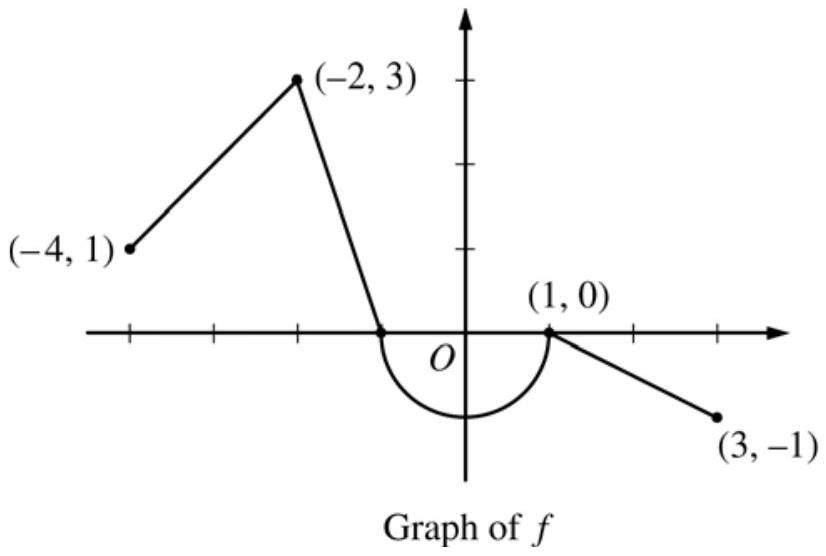
\includegraphics[width=0.6\linewidth]{figures/bc-2012_fig1.jpg}
\end{center}
Let $f$ be the continuous function defined on $[-4,3]$ whose graph, consisting of three line segments and a semicircle centered at the origin, is given above. Let $g$ be the function given by $g(x)=\int_{1}^{x} f(t) d t$.\\
\begin{parts}
\part Find the values of $g(2)$ and $g(-2)$.
\part For each of $g^{\prime}(-3)$ and $g^{\prime \prime}(-3)$, find the value or state that it does not exist.
\part Find the $x$-coordinate of each point at which the graph of $g$ has a horizontal tangent line. For each of these points, determine whether $g$ has a relative minimum, relative maximum, or neither a minimum nor a maximum at the point. Justify your answers.
\part For $-4<x<3$, find all values of $x$ for which the graph of $g$ has a point of inflection. Explain your reasoning.
\end{parts}
\begin{solution}
\begin{parts}
\part $\quad g(2)=\int_{1}^{2} f(t) d t=-\frac{1}{2}(1)\left(\frac{1}{2}\right)=-\frac{1}{4}$

\[\begin{aligned}
g(-2) & =\int_{1}^{-2} f(t) d t=-\int_{-2}^{1} f(t) d t \\
& =-\left(\frac{3}{2}-\frac{\pi}{2}\right)=\frac{\pi}{2}-\frac{3}{2}
\end{aligned}\]
\part $g^{\prime}(x)=f(x) \Rightarrow g^{\prime}(-3)=f(-3)=2$\\
$g^{\prime \prime}(x)=f^{\prime}(x) \Rightarrow g^{\prime \prime}(-3)=f^{\prime}(-3)=1$
\part The graph of $g$ has a horizontal tangent line where $g^{\prime}(x)=f(x)=0$. This occurs at $x=-1$ and $x=1$.\\
$3:\left\{\begin{array}{l}1: \text { considers } g^{\prime}(x)=0 \\ 1: x=-1 \text { and } x=1 \\ 1: \text { answers with justifications }\end{array}\right.$\\
$g^{\prime}(x)$ changes sign from positive to negative at $x=-1$. Therefore, $g$ has a relative maximum at $x=-1$.\\
$g^{\prime}(x)$ does not change sign at $x=1$. Therefore, $g$ has neither a relative maximum nor a relative minimum at $x=1$.
\part The graph of $g$ has a point of inflection at each of $x=-2, x=0$, and $x=1$ because $g^{\prime \prime}(x)=f^{\prime}(x)$ changes $2:\left\{\begin{array}{l}1: \text { answer } \\ 1: \text { explanation }\end{array}\right.$ sign at each of these values.

\begin{center}
\end{center}
\end{parts}
\end{solution}

\question
% Q4 | 2012 Calculus BC | Part B | Calculator Prohibited
\begin{center}
\begin{tabular}{|c||c|c|c|c|c|}
\hline
$x$ & 1 & 1.1 & 1.2 & 1.3 & 1.4 \\
\hline
$f^{\prime}(x)$ & 8 & 10 & 12 & 13 & 14.5 \\
\hline
\end{tabular}
\end{center}
The function $f$ is twice differentiable for $x>0$ with $f(1)=15$ and $f^{\prime \prime}(1)=20$. Values of $f^{\prime}$, the derivative of $f$, are given for selected values of $x$ in the table above.\\
\begin{parts}
\part Write an equation for the line tangent to the graph of $f$ at $x=1$. Use this line to approximate $f(1.4)$.
\part Use a midpoint Riemann sum with two subintervals of equal length and values from the table to approximate $\int_{1}^{1.4} f^{\prime}(x) d x$. Use the approximation for $\int_{1}^{1.4} f^{\prime}(x) d x$ to estimate the value of $f(1.4)$. Show the computations that lead to your answer.
\part Use Euler's method, starting at $x=1$ with two steps of equal size, to approximate $f(1.4)$. Show the computations that lead to your answer.
\part Write the second-degree Taylor polynomial for $f$ about $x=1$. Use the Taylor polynomial to approximate $f(1.4)$.
\end{parts}
\begin{solution}
\begin{parts}
\part $f(1)=15, f^{\prime}(1)=8$

An equation for the tangent line is\\
$y=15+8(x-1)$.

\[f(1.4) \approx 15+8(1.4-1)=18.2\]
\part $\int_{1}^{1.4} f^{\prime}(x) d x \approx(0.2)(10)+(0.2)(13)=4.6$

\begin{align*}& f(1.4)=f(1)+\int_{1}^{1.4} f^{\prime}(x) d x \\
& f(1.4) \approx 15+4.6=19.6\end{align*}
\part $f(1.2) \approx f(1)+(0.2)(8)=16.6$

\[f(1.4) \approx 16.6+(0.2)(12)=19.0\]
\part $T_{2}(x)=15+8(x-1)+\frac{20}{2!}(x-1)^{2}$

\[=15+8(x-1)+10(x-1)^{2}\]

\[f(1.4) \approx 15+8(1.4-1)+10(1.4-1)^{2}=19.8\]
\end{parts}
\par\medskip
\textbf{Rubric:}\par
\begin{parts}
\part $2:\left\{\begin{array}{l}
1: \text { tangent line } \\
1: \text { approximation }
\end{array}\right.$
\part $3:\left\{\begin{array}{l}
1: \text { midpoint Riemann sum } \\
1: \text { Fundamental Theorem of Calculus } \\
1: \text { answer }
\end{array}\right.$
\part $2:\left\{\begin{array}{l}
1: \text { Euler's method with two steps } \\
1: \text { answer }
\end{array}\right.$
\part $2:\left\{\begin{array}{l}
1: \text { Taylor polynomial } \\
1: \text { approximation }
\end{array}\right.$
\end{parts}
\end{solution}

\question
% Q5 | 2012 Calculus BC | Part B | Calculator Prohibited
The rate at which a baby bird gains weight is proportional to the difference between its adult weight and its current weight. At time $t=0$, when the bird is first weighed, its weight is 20 grams. If $B(t)$ is the weight of the bird, in grams, at time $t$ days after it is first weighed, then
\[\frac{d B}{d t}=\frac{1}{5}(100-B) .\]

Let $y=B(t)$ be the solution to the differential equation above with initial condition $B(0)=20$.\\
\begin{parts}
\part Is the bird gaining weight faster when it weighs 40 grams or when it weighs 70 grams? Explain your reasoning.
\part Find $\frac{d^{2} B}{d t^{2}}$ in terms of $B$. Use $\frac{d^{2} B}{d t^{2}}$ to explain why the graph of $B$ cannot resemble the following graph.\\
\begin{center}
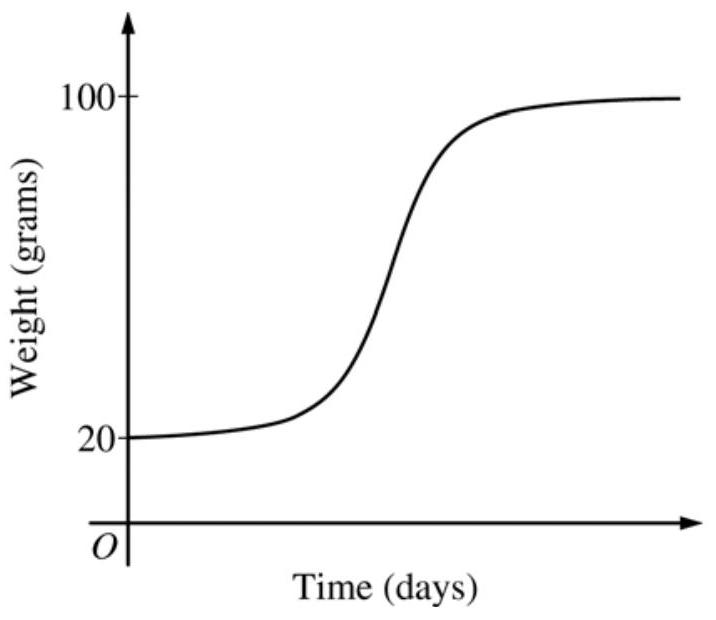
\includegraphics[width=0.6\linewidth]{figures/bc-2012_fig2.jpg}
\end{center}
\part Use separation of variables to find $y=B(t)$, the particular solution to the differential equation with initial condition $B(0)=20$.
\end{parts}
\begin{solution}
\begin{parts}
\part $\left.\frac{d B}{d t}\right|_{B=40}=\frac{1}{5}(60)=12$

\[\left.\frac{d B}{d t}\right|_{B=70}=\frac{1}{5}(30)=6\]

Because $\left.\frac{d B}{d t}\right|_{B=40}>\left.\frac{d B}{d t}\right|_{B=70}$, the bird is gaining weight faster when it weighs 40 grams.
\part $\frac{d^{2} B}{d t^{2}}=-\frac{1}{5} \frac{d B}{d t}=-\frac{1}{5} \cdot \frac{1}{5}(100-B)=-\frac{1}{25}(100-B)$

Therefore, the graph of $B$ is concave down for\\
$2:\left\{\begin{array}{l}1: \text { uses } \frac{d B}{d t} \\ 1: \text { answer with reason }\end{array}\right.$\\
$2:\left\{\begin{array}{l}1: \frac{d^{2} B}{d t^{2}} \text { in terms of } B \\ 1: \text { explanation }\end{array}\right. 20 \leq B<100$. A portion of the given graph is concave up.
\part $\frac{d B}{d t}=\frac{1}{5}(100-B)$

\begin{align*}& \int \frac{1}{100-B} d B=\int \frac{1}{5} d t \\
& -\ln |100-B|=\frac{1}{5} t+C\end{align*}

Because $20 \leq B<100,|100-B|=100-B$.

\[-\ln (100-20)=\frac{1}{5}(0)+C \Rightarrow-\ln (80)=C\]

$100-B=80 e^{-t / 5}$

\[B(t)=100-80 e^{-t / 5}, \quad t \geq 0\]
\end{parts}
\par\medskip
\textbf{Rubric:}\par
\begin{parts}
\part $5:\left\{\begin{array}{l}1: \text { separates variables } \\ 1: \text { antiderivative of } \frac{1}{100-B} \text { term } \\ 1: \text { antiderivative of } \frac{1}{5} \text { term } \\ 1: \text { uses initial condition } \\ 1: \text { solves for } B(t)\end{array}\right.$
\part Note: $\max 2 / 5[1-1-0-0-0]$ if no constant of integration
\part Note: $0 / 5$ if no separation of variables
\end{parts}
\end{solution}

\question
% Q6 | 2012 Calculus BC | Part B | Calculator Prohibited
The function $g$ has derivatives of all orders, and the Maclaurin series for $g$ is
\[\sum_{n=0}^{\infty}(-1)^{n} \frac{x^{2 n+1}}{2 n+3}=\frac{x}{3}-\frac{x^{3}}{5}+\frac{x^{5}}{7}-\cdots\]
\begin{parts}
\part Using the ratio test, determine the interval of convergence of the Maclaurin series for $g$.
\part The Maclaurin series for $g$ evaluated at $x=\frac{1}{2}$ is an alternating series whose terms decrease in absolute value to 0 . The approximation for $g\left(\frac{1}{2}\right)$ using the first two nonzero terms of this series is $\frac{17}{120}$. Show that this approximation differs from $g\left(\frac{1}{2}\right)$ by less than $\frac{1}{200}$.
\part Write the first three nonzero terms and the general term of the Maclaurin series for $g^{\prime}(x)$.
\end{parts}
\begin{solution}
\begin{parts}
\part $\left|\frac{x^{2 n+3}}{2 n+5} \cdot \frac{2 n+3}{x^{2 n+1}}\right|=\left(\frac{2 n+3}{2 n+5}\right) \cdot x^{2}$

\[\begin{aligned}
& \lim _{n \rightarrow \infty}\left(\frac{2 n+3}{2 n+5}\right) \cdot x^{2}=x^{2} \\
& x^{2}<1 \Rightarrow-1<x<1
\end{aligned}\]

The series converges when $-1<x<1$.

When $x=-1$, the series is $-\frac{1}{3}+\frac{1}{5}-\frac{1}{7}+\frac{1}{9}-\cdots$\\
This series converges by the Alternating Series Test.

When $x=1$, the series is $\frac{1}{3}-\frac{1}{5}+\frac{1}{7}-\frac{1}{9}+\cdots$\\
This series converges by the Alternating Series Test.\\
Therefore, the interval of convergence is $-1 \leq x \leq 1$.
\part $\left|g\left(\frac{1}{2}\right)-\frac{17}{120}\right|<\frac{\left(\frac{1}{2}\right)^{5}}{7}=\frac{1}{224}<\frac{1}{200}$

\[5:\left\{\begin{array}{l}
1: \text { sets up ratio } \\
1: \text { computes limit of ratio } \\
1: \text { identifies interior of } \\
\quad \text { interval of convergence } \\
1: \text { considers both endpoints } \\
1: \text { analysis and interval of convergence }
\end{array}\right.\]
\part $g^{\prime}(x)=\frac{1}{3}-\frac{3}{5} x^{2}+\frac{5}{7} x^{4}+\cdots+(-1)^{n}\left(\frac{2 n+1}{2 n+3}\right) x^{2 n}+\cdots$
\end{parts}
\par\medskip
\textbf{Rubric:}\par
\begin{parts}
\part $2:\left\{\begin{array}{l}
1: \text { uses the third term as an error bound } \\
1: \text { error bound }
\end{array}\right.$
\part $2:\left\{\begin{array}{l}
1: \text { first three terms } \\
1: \text { general term }
\end{array}\right.$
\end{parts}
\end{solution}

\end{questions}

\section*{2013 AP Calculus BC}

\begin{questions}

\question
% Q1 | 2013 Calculus BC | Part A | Calculator Active
On a certain workday, the rate, in tons per hour, at which unprocessed gravel arrives at a gravel processing plant is modeled by $G(t)=90+45 \cos \left(\frac{t^{2}}{18}\right)$, where $t$ is measured in hours and $0 \leq t \leq 8$. At the beginning of the workday $(t=0)$, the plant has 500 tons of unprocessed gravel. During the hours of operation, $0 \leq t \leq 8$, the plant processes gravel at a constant rate of 100 tons per hour.\\
\begin{parts}
\part Find $G^{\prime}(5)$. Using correct units, interpret your answer in the context of the problem.
\part Find the total amount of unprocessed gravel that arrives at the plant during the hours of operation on this workday.
\part Is the amount of unprocessed gravel at the plant increasing or decreasing at time $t=5$ hours? Show the work that leads to your answer.
\part What is the maximum amount of unprocessed gravel at the plant during the hours of operation on this workday? Justify your answer.
\end{parts}
\begin{solution}
\begin{parts}
\part $G^{\prime}(5)=-24.588$ (or -24.587 )

The rate at which gravel is arriving is decreasing by 24.588 (or 24.587) tons per hour per hour at time $t=5$ hours.
\part $\int_{0}^{8} G(t) d t=825.551$ tons
\part $G(5)=98.140764<100$

At time $t=5$, the rate at which unprocessed gravel is arriving is less than the rate at which it is being processed.\\
Therefore, the amount of unprocessed gravel at the plant is decreasing at time $t=5$.
\part The amount of unprocessed gravel at time $t$ is given by

\begin{align*}& A(t)=500+\int_{0}^{t}(G(s)-100) d s \\
& A^{\prime}(t)=G(t)-100=0 \Rightarrow t=4.923480\end{align*}

\begin{center}
\begin{tabular}{c|c}
$t$ & $A(t)$ \\
\hline
0 & 500 \\
4.92348 & 635.376123 \\
8 & 525.551089 \\
\end{tabular}
\end{center}

The maximum amount of unprocessed gravel at the plant during
\end{parts}
\par\medskip
\textbf{Rubric:}\par
\begin{parts}
\part $1: G^{\prime}(5)$
\end{parts}
\end{solution}

\question
% Q2 | 2013 Calculus BC | Part A | Calculator Active
\begin{center}
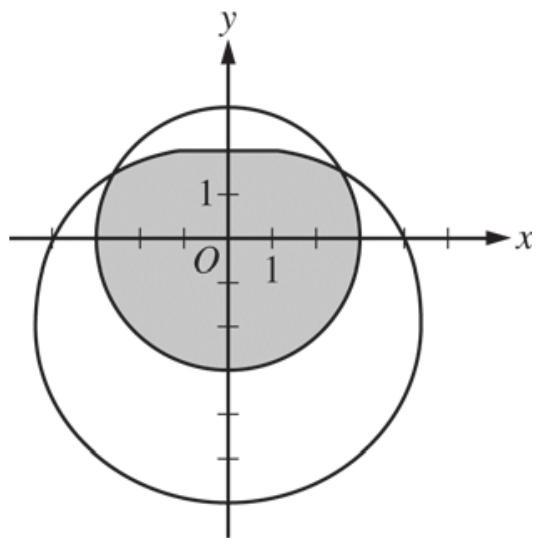
\includegraphics[width=0.6\linewidth]{figures/bc-2013_fig1.jpg}
\end{center}
The graphs of the polar curves $r=3$ and $r=4-2 \sin \theta$ are shown in the figure above. The curves intersect when $\theta=\frac{\pi}{6}$ and $\theta=\frac{5 \pi}{6}$.\\
\begin{parts}
\part Let $S$ be the shaded region that is inside the graph of $r=3$ and also inside the graph of $r=4-2 \sin \theta$. Find the area of $S$.
\part A particle moves along the polar curve $r=4-2 \sin \theta$ so that at time $t$ seconds, $\theta=t^{2}$. Find the time $t$ in the interval $1 \leq t \leq 2$ for which the $x$-coordinate of the particle's position is -1 .
\part For the particle described in part (b), find the position vector in terms of $t$. Find the velocity vector at time $t=1.5$.
\end{parts}
\begin{solution}
\begin{parts}
\part Area $=6 \pi+\frac{1}{2} \int_{\pi / 6}^{5 \pi / 6}(4-2 \sin \theta)^{2} d \theta=24.709$ (or 24.708)
\part $x=r \cos \theta \Rightarrow x(\theta)=(4-2 \sin \theta) \cos \theta$

\[\begin{aligned}
& x(t)=\left(4-2 \sin \left(t^{2}\right)\right) \cos \left(t^{2}\right) \\
& x(t)=-1 \text { when } t=1.428(\text { or } 1.427)
\end{aligned}\]
\part $y=r \sin \theta \Rightarrow y(\theta)=(4-2 \sin \theta) \sin \theta$

\[y(t)=\left(4-2 \sin \left(t^{2}\right)\right) \sin \left(t^{2}\right)\]

\[\begin{aligned}
& \text { Position vector }=\langle x(t), y(t)\rangle \\
& =\left\langle\left(4-2 \sin \left(t^{2}\right)\right) \cos \left(t^{2}\right),\left(4-2 \sin \left(t^{2}\right)\right) \sin \left(t^{2}\right)\right\rangle
\end{aligned} \begin{aligned}
v(1.5)= & \left\langle x^{\prime}(1.5), y^{\prime}(1.5)\right\rangle \\
= & \langle-8.072,-1.673\rangle(\text { or }\langle-8.072,-1.672\rangle)
\end{aligned} \text { }\]
\end{parts}
\par\medskip
\textbf{Rubric:}\par
\begin{parts}
\part $3:\left\{\begin{array}{l}
2: \text { position vector } \\
1: \text { velocity vector }
\end{array}\right.$
\part $3:\left\{\begin{array}{l}
1: \text { integrand } \\
1: \text { limits and constant } \\
1: \text { answer }
\end{array}\right.$
\part $3:\left\{\begin{array}{l}1: x(\theta) \text { or } x(t) \\ 1: x(\theta)=-1 \text { or } x(t)=-1 \\ 1: \text { answer }\end{array}\right.$
\end{parts}
\end{solution}

\question
% Q3 | 2013 Calculus BC | Part B | Calculator Prohibited
\begin{center}
\begin{tabular}{|c||c|c|c|c|c|c|c|}
\hline
\begin{tabular}{c}
$t$ \\
(minutes) \\
\end{tabular} & 0 & 1 & 2 & 3 & 4 & 5 & 6 \\
\hline
\begin{tabular}{c}
$C(t)$ \\
(ounces) \\
\end{tabular} & 0 & 5.3 & 8.8 & 11.2 & 12.8 & 13.8 & 14.5 \\
\hline
\end{tabular}
\end{center}
Hot water is dripping through a coffeemaker, filling a large cup with coffee. The amount of coffee in the cup at time $t, 0 \leq t \leq 6$, is given by a differentiable function $C$, where $t$ is measured in minutes. Selected values of $C(t)$, measured in ounces, are given in the table above.\\
\begin{parts}
\part Use the data in the table to approximate $C^{\prime}(3.5)$. Show the computations that lead to your answer, and indicate units of measure.
\part Is there a time $t, 2 \leq t \leq 4$, at which $C^{\prime}(t)=2$ ? Justify your answer.
\part Use a midpoint sum with three subintervals of equal length indicated by the data in the table to approximate the value of $\frac{1}{6} \int_{0}^{6} C(t) d t$. Using correct units, explain the meaning of $\frac{1}{6} \int_{0}^{6} C(t) d t$ in the context of the problem.
\part The amount of coffee in the cup, in ounces, is modeled by $B(t)=16-16 e^{-0.4 t}$. Using this model, find the rate at which the amount of coffee in the cup is changing when $t=5$.
\end{parts}
\begin{solution}
\begin{parts}
\part $C^{\prime}(3.5) \approx \frac{C(4)-C(3)}{4-3}=\frac{12.8-11.2}{1}=1.6$ ounces $/ \mathrm{min}$
\part $C$ is differentiable $\Rightarrow C$ is continuous (on the closed interval) $\frac{C(4)-C(2)}{4-2}=\frac{12.8-8.8}{2}=2$\\
Therefore, by the Mean Value Theorem, there is at least one time $t, 2<t<4$, for which $C^{\prime}(t)=2$.
\part $\frac{1}{6} \int_{0}^{6} C(t) d t \approx \frac{1}{6}[2 \cdot C(1)+2 \cdot C(3)+2 \cdot C(5)]$

\begin{align*}& =\frac{1}{6}(2 \cdot 5.3+2 \cdot 11.2+2 \cdot 13.8) \\
& =\frac{1}{6}(60.6)=10.1 \text { ounces }\end{align*}

$\frac{1}{6} \int_{0}^{6} C(t) d t$ is the average amount of coffee in the cup, in ounces, over the time interval $0 \leq t \leq 6$ minutes.
\part $B^{\prime}(t)=-16(-0.4) e^{-0.4 t}=6.4 e^{-0.4 t} B^{\prime}(5)=6.4 e^{-0.4(5)}=\frac{6.4}{e^{2}}$ ounces $/ \mathrm{min}$
\end{parts}
\par\medskip
\textbf{Rubric:}\par
\begin{parts}
\part $2:\left\{\begin{array}{l}1: \text { approximation } \\ 1: \text { units }\end{array}\right.$
\part $2:\left\{\begin{array}{l}1: \frac{C(4)-C(2)}{4-2} \\ 1: \text { conclusion, using MVT }\end{array}\right.$
\part $3:\left\{\begin{array}{l}1: \text { midpoint sum } \\ 1: \text { approximation } \\ 1: \text { interpretation }\end{array}\right.$
\part $2:\left\{\begin{array}{l}1: B^{\prime}(t) \\ 1: B^{\prime}(5)\end{array}\right.$
\end{parts}
\end{solution}

\question
% Q4 | 2013 Calculus BC | Part B | Calculator Prohibited
\begin{center}
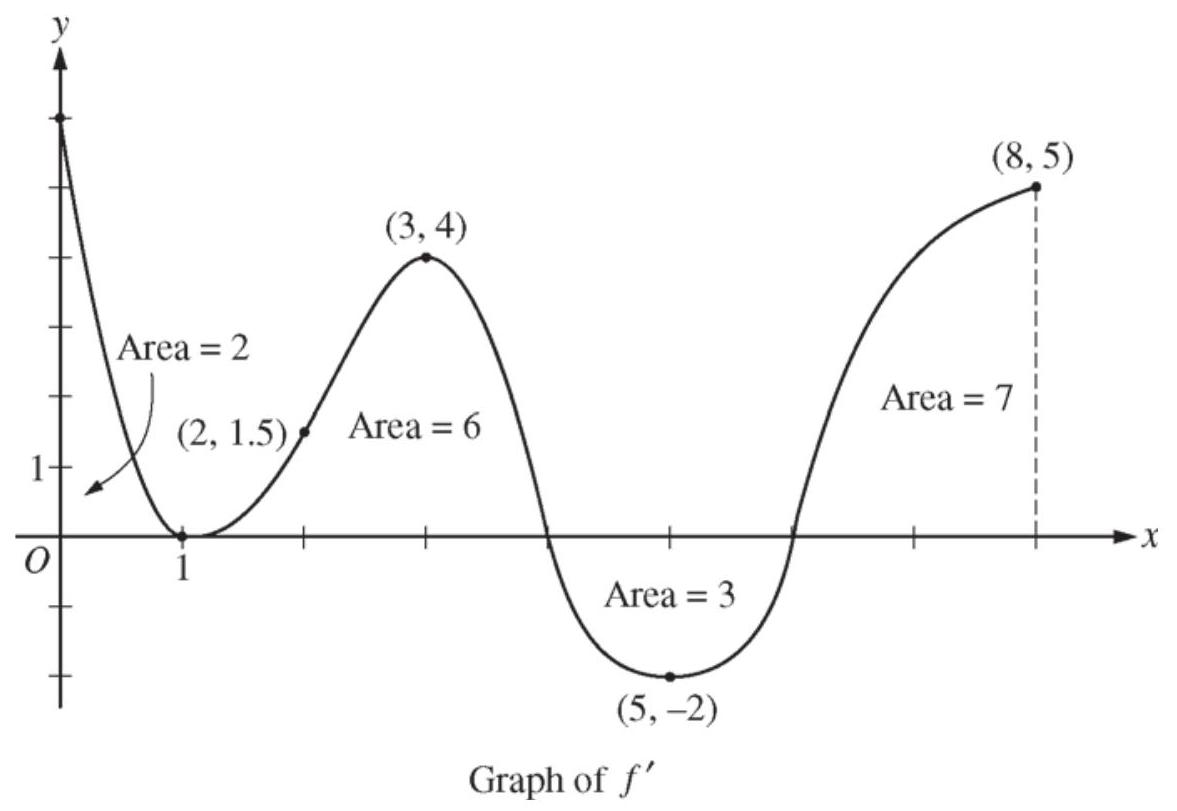
\includegraphics[width=0.6\linewidth]{figures/bc-2013_fig2.jpg}
\end{center}
The figure above shows the graph of $f^{\prime}$, the derivative of a twice-differentiable function $f$, on the closed interval $0 \leq x \leq 8$. The graph of $f^{\prime}$ has horizontal tangent lines at $x=1, x=3$, and $x=5$. The areas of the regions between the graph of $f^{\prime}$ and the $x$-axis are labeled in the figure. The function $f$ is defined for all real numbers and satisfies $f(8)=4$.\\
\begin{parts}
\part Find all values of $x$ on the open interval $0<x<8$ for which the function $f$ has a local minimum. Justify your answer.
\part Determine the absolute minimum value of $f$ on the closed interval $0 \leq x \leq 8$. Justify your answer.
\part On what open intervals contained in $0<x<8$ is the graph of $f$ both concave down and increasing? Explain your reasoning.
\part The function $g$ is defined by $g(x)=(f(x))^{3}$. If $f(3)=-\frac{5}{2}$, find the slope of the line tangent to the graph of $g$ at $x=3$.
\end{parts}
\begin{solution}
\begin{parts}
\part $x=6$ is the only critical point at which $f^{\prime}$ changes sign from negative to positive. Therefore, $f$ has a local minimum at $x=6$.
\part From part (a), the absolute minimum occurs either at $x=6$ or at an endpoint.

\begin{align*}f(0) & =f(8)+\int_{8}^{0} f^{\prime}(x) d x \\
& =f(8)-\int_{0}^{8} f^{\prime}(x) d x=4-12=-8 \\
f(6) & =f(8)+\int_{8}^{6} f^{\prime}(x) d x \\
& =f(8)-\int_{6}^{8} f^{\prime}(x) d x=4-7=-3 \\
f(8) & =4\end{align*}

The absolute minimum value of $f$ on the closed interval $[0,8]$ is -8 .
\part The graph of $f$ is concave down and increasing on $0<x<1$ and $3<x<4$, because $f^{\prime}$ is decreasing and positive on these intervals.
\part $g^{\prime}(x)=3[f(x)]^{2} \cdot f^{\prime}(x)$

\[g^{\prime}(3)=3[f(3)]^{2} \cdot f^{\prime}(3)=3\left(-\frac{5}{2}\right)^{2} \cdot 4=75\]
\end{parts}
\par\medskip
\textbf{Rubric:}\par
\begin{parts}
\part 1 : answer with justification
\part $3:\left\{\begin{array}{l}
1: \operatorname{considers} x=0 \text { and } x=6 \\
1: \text { answer } \\
1: \text { justification }
\end{array}\right.$
\part $2:\left\{\begin{array}{l}
1: \text { answer } \\
1: \text { explanation }
\end{array}\right.$
\part $3:\left\{\begin{array}{l}
2: g^{\prime}(x) \\
1: \text { answer }
\end{array}\right.$
\end{parts}
\end{solution}

\question
% Q5 | 2013 Calculus BC | Part B | Calculator Prohibited
Consider the differential equation $\frac{d y}{d x}=y^{2}(2 x+2)$. Let $y=f(x)$ be the particular solution to the differential equation with initial condition $f(0)=-1$.\\
\begin{parts}
\part Find $\lim _{x \rightarrow 0} \frac{f(x)+1}{\sin x}$. Show the work that leads to your answer.
\part Use Euler's method, starting at $x=0$ with two steps of equal size, to approximate $f\left(\frac{1}{2}\right)$.
\part Find $y=f(x)$, the particular solution to the differential equation with initial condition $f(0)=-1$.
\end{parts}
\begin{solution}
\begin{parts}
\part $f(0)=-1, \quad f^{\prime}(0)=(-1)^{2}(2 \cdot 0+2)=2$

$\lim_{x \rightarrow 0} \frac{f(x)+1}{\sin x}=\frac{f^{\prime}(0)}{\cos 0}=\frac{2}{1}=2$
\part $f(0)=-1, \quad \left.\frac{d y}{d x}\right|_{x=0}=(-1)^{2}(2)=2$

$f(0.25) \approx-1+2(0.25)=-0.5$

$\left.\frac{d y}{d x}\right|_{x=0.25}=(-0.5)^{2}(2(0.25)+2)=0.25 \cdot 2.5=0.625$

$f(0.5) \approx-0.5+0.625(0.25)=-0.34375$
\part $\frac{d y}{y^{2}}=(2 x+2) d x$

$\int y^{-2} d y=\int(2 x+2) d x$

$-\frac{1}{y}=x^{2}+2 x+C$

$f(0)=-1: \quad 1=0+0+C \Rightarrow C=1$

$-\frac{1}{y}=x^{2}+2 x+1=(x+1)^{2}$

$f(x)=-\frac{1}{(x+1)^{2}}$
\end{parts}
\par\medskip
\textbf{Rubric:}\par
\begin{parts}
\part Note: This solution is valid for $x>-1$.
\part $2:\left\{\begin{array}{l}1: \lim _{x \rightarrow 0} \frac{f(x)+1}{\sin x} \\ 1: \text { answer }\end{array}\right.$
\part $3:\left\{\begin{array}{l}1: \text { Euler's method with two steps } \\ 1: y(0.25) \\ 1: y(0.5)\end{array}\right.$
\part $5:\left\{\begin{array}{l}1: \text { separates variables } \\ 1: \text { antiderivatives } \\ 1: \text { constant of integration } \\ 1: \text { uses initial condition } \\ 1: \text { solves for } f(x)\end{array}\right.$
\end{parts}
\end{solution}

\question
% Q6 | 2013 Calculus BC | Part B | Calculator Prohibited
A function $f$ has derivatives of all orders at $x=0$. Let $P_{n}(x)$ denote the $n$ th-degree Taylor polynomial for $f$ about $x=0$.\\
\begin{parts}
\part It is known that $f(0)=-4$ and that $P_{1}\left(\frac{1}{2}\right)=-3$. Show that $f^{\prime}(0)=2$.
\part It is known that $f^{\prime \prime}(0)=-\frac{2}{3}$ and $f^{\prime \prime \prime}(0)=\frac{1}{3}$. Find $P_{3}(x)$.
\part The function $h$ has first derivative given by $h^{\prime}(x)=f(2 x)$. It is known that $h(0)=7$. Find the third-degree Taylor polynomial for $h$ about $x=0$.
\end{parts}
\begin{solution}
\begin{parts}
\part $P_{1}(x)=f(0)+f^{\prime}(0) x=-4+f^{\prime}(0) x$

\[\begin{aligned}
& P_{1}\left(\frac{1}{2}\right)=-4+f^{\prime}(0) \cdot \frac{1}{2}=-3 \\
& f^{\prime}(0) \cdot \frac{1}{2}=1 \\
& f^{\prime}(0)=2
\end{aligned}\]
\part $P_{3}(x)=-4+2 x+\left(-\frac{2}{3}\right) \cdot \frac{x^{2}}{2!}+\frac{1}{3} \cdot \frac{x^{3}}{3!}$

\[=-4+2 x-\frac{1}{3} x^{2}+\frac{1}{18} x^{3}\]
\part Let $Q_{n}(x)$ denote the Taylor polynomial of degree $n$ for $h$ about $x=0$.

\begin{align*}& h^{\prime}(x)=f(2 x) \Rightarrow Q_{3}^{\prime}(x)=-4+2(2 x)-\frac{1}{3}(2 x)^{2} \\
& Q_{3}(x)=-4 x+4 \cdot \frac{x^{2}}{2}-\frac{4}{3} \cdot \frac{x^{3}}{3}+C ; C=Q_{3}(0)=h(0)=7 \\
& Q_{3}(x)=7-4 x+2 x^{2}-\frac{4}{9} x^{3}\end{align*}

OR

\begin{align*}& h^{\prime}(x)=f(2 x), h^{\prime \prime}(x)=2 f^{\prime}(2 x), h^{\prime \prime \prime}(x)=4 f^{\prime \prime}(2 x) \\
& h^{\prime}(0)=f(0)=-4, h^{\prime \prime}(0)=2 f^{\prime}(0)=4, h^{\prime \prime \prime}(0)=4 f^{\prime \prime}(0)=-\frac{8}{3} \\
& Q_{3}(x)=7-4 x+4 \cdot \frac{x^{2}}{2!}-\frac{8}{3} \cdot \frac{x^{3}}{3!}=7-4 x+2 x^{2}-\frac{4}{9} x^{3}\end{align*}
\end{parts}
\par\medskip
\textbf{Rubric:}\par
\begin{parts}
\part $2:\left\{\begin{array}{l}
1: \text { uses } P_{1}(x) \\
1: \text { verifies } f^{\prime}(0)=2
\end{array}\right.$
\part $3:\left\{\begin{array}{l}
1: \text { first two terms } \\
1: \text { third term } \\
1: \text { fourth term }
\end{array}\right.$
\part $4:\left\{\begin{array}{l}
2: \text { applies } h^{\prime}(x)=f(2 x) \\
1: \text { constant term } \\
1: \text { remaining terms }
\end{array}\right.$
\end{parts}
\end{solution}

\end{questions}

\section*{2014 AP Calculus BC}

\begin{questions}

\question
% Q1 | 2014 Calculus BC | Part A | Calculator Active
Grass clippings are placed in a bin, where they decompose. For $0 \leq t \leq 30$, the amount of grass clippings remaining in the bin is modeled by $A(t)=6.687(0.931)^{t}$, where $A(t)$ is measured in pounds and $t$ is measured in days.\\
\begin{parts}
\part Find the average rate of change of $A(t)$ over the interval $0 \leq t \leq 30$. Indicate units of measure.
\part Find the value of $A^{\prime}(15)$. Using correct units, interpret the meaning of the value in the context of the problem.
\part Find the time $t$ for which the amount of grass clippings in the bin is equal to the average amount of grass clippings in the bin over the interval $0 \leq t \leq 30$.
\part For $t>30, L(t)$, the linear approximation to $A$ at $t=30$, is a better model for the amount of grass clippings remaining in the bin. Use $L(t)$ to predict the time at which there will be 0.5 pound of grass clippings remaining in the bin. Show the work that leads to your answer.
\end{parts}
\begin{solution}
\begin{parts}
\part $\frac{A(30)-A(0)}{30-0}=-0.197$ (or -0.196 ) lbs/day
\part $A^{\prime}(15)=-0.164$ (or -0.163 )

The amount of grass clippings in the bin is decreasing at a rate of 0.164 (or 0.163 ) lbs/day at time $t=15$ days.
\part $A(t)=\frac{1}{30} \int_{0}^{30} A(t) d t \Rightarrow t=12.415$ (or 12.414)
\part $L(t)=A(30)+A^{\prime}(30) \cdot(t-30)$\\
$A^{\prime}(30)=-0.055976$\\
$A(30)=0.782928$\\
$L(t)=0.5 \Rightarrow t=35.054$
\end{parts}
\par\medskip
\textbf{Rubric:}\par
\begin{parts}
\part 1 : answer with units
\part $2:\left\{\begin{array}{l}1: A^{\prime}(15) \\ 1: \text { interpretation }\end{array}\right.$
\part $2:\left\{\begin{array}{l}1: \frac{1}{30} \int_{0}^{30} A(t) d t \\ 1: \text { answer }\end{array}\right.$
\part $4:\left\{\begin{array}{l}2: \text { expression for } L(t) \\ 1: L(t)=0.5 \\ 1: \text { answer }\end{array}\right.$
\end{parts}
\end{solution}

\question
% Q2 | 2014 Calculus BC | Part A | Calculator Active
\begin{center}
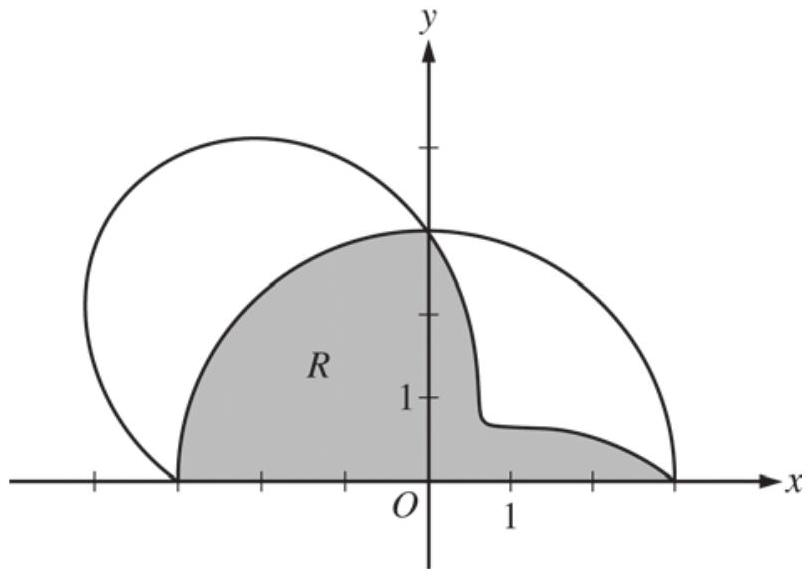
\includegraphics[width=0.6\linewidth]{figures/bc-2014_fig1.jpg}
\end{center}
The graphs of the polar curves $r=3$ and $r=3-2 \sin (2 \theta)$ are shown in the figure above for $0 \leq \theta \leq \pi$.\\

\begin{center}
  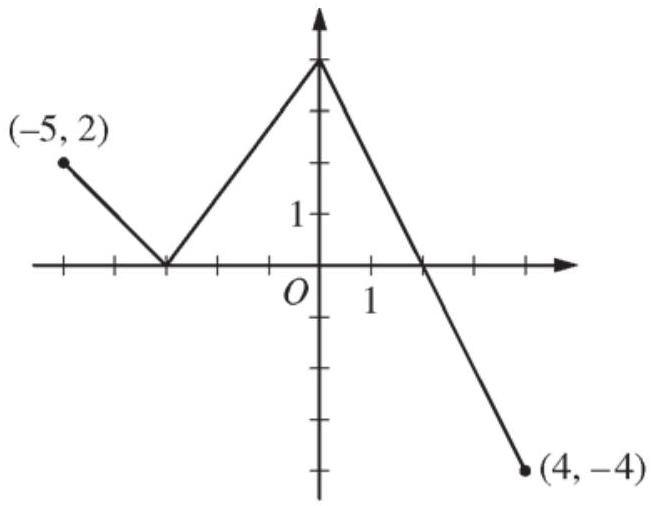
\includegraphics[width=0.6\linewidth]{figures/bc-2014_fig2.jpg}
\end{center}
\begin{parts}
\part Let $R$ be the shaded region that is inside the graph of $r=3$ and inside the graph of $r=3-2 \sin (2 \theta)$. Find the area of $R$.
\part For the curve $r=3-2 \sin (2 \theta)$, find the value of $\frac{d x}{d \theta}$ at $\theta=\frac{\pi}{6}$.
\part The distance between the two curves changes for $0<\theta<\frac{\pi}{2}$. Find the rate at which the distance between the two curves is changing with respect to $\theta$ when $\theta=\frac{\pi}{3}$.
\part A particle is moving along the curve $r=3-2 \sin (2 \theta)$ so that $\frac{d \theta}{d t}=3$ for all times $t \geq 0$. Find the value of $\frac{d r}{d t}$ at $\theta=\frac{\pi}{6}$.
\end{parts}
\begin{solution}
\begin{parts}
\part Area $=\frac{9 \pi}{4}+\frac{1}{2} \int_{0}^{\pi / 2}(3-2 \sin (2 \theta))^{2} d \theta$

\[\text { = } 9.708(\text { or } 9.707)\]
\part $x=(3-2 \sin (2 \theta)) \cos \theta$

\[\left.\frac{d x}{d \theta}\right|_{\theta=\pi / 6}=-2.366\]
\part The distance between the two curves is

\begin{align*}& D=3-(3-2 \sin (2 \theta))=2 \sin (2 \theta) \\
& \left.\frac{d D}{d \theta}\right|_{\theta=\pi / 3}=-2\end{align*}
\part $\frac{d r}{d t}=\frac{d r}{d \theta} \cdot \frac{d \theta}{d t}=\frac{d r}{d \theta} \cdot 3$

\[\left.\frac{d r}{d t}\right|_{\theta=\pi / 6}=(-2)(3)=-6\]
\end{parts}
\par\medskip
\textbf{Rubric:}\par
\begin{parts}
\part $2:\left\{\begin{array}{l}
1: \text { expression for distance } \\
1: \text { answer }
\end{array}\right.$
\part $2:\left\{\begin{array}{l}
1: \text { chain rule with respect to } t \\
1: \text { answer }
\end{array}\right.$
\end{parts}
\end{solution}

\question
% Q3 | 2014 Calculus BC | Part B | Calculator Prohibited
The function $f$ is defined on the closed interval $[-5,4]$. The graph of $f$ consists of three line segments and is shown in the figure below. Let $g$ be the function defined by $g(x)=\int_{-3}^{x} f(t) d t$.\\
\begin{parts}
\part Find $g(3)$.
\part On what open intervals contained in $-5<x<4$ is the graph of $g$ both increasing and concave down? Give a reason for your answer.
\part The function $h$ is defined by $h(x)=\frac{g(x)}{5 x}$. Find $h^{\prime}(3)$.
\part The function $p$ is defined by $p(x)=f\left(x^{2}-x\right)$. Find the slope of the line tangent to the graph of $p$ at the point where $x=-1$.
\end{parts}
\begin{solution}
\begin{parts}
\part $g(3)=\int_{-3}^{3} f(t) d t=6+4-1=9$
\part $g^{\prime}(x)=f(x)$

The graph of $g$ is increasing and concave down on the intervals $-5<x<-3$ and $0<x<2$ because $g^{\prime}=f$ is positive and decreasing on these intervals.
\part $h^{\prime}(x)=\frac{5 x g^{\prime}(x)-g(x) 5}{(5 x)^{2}}=\frac{5 x g^{\prime}(x)-5 g(x)}{25 x^{2}}$

\begin{align*}h^{\prime}(3) & =\frac{(5)(3) g^{\prime}(3)-5 g(3)}{25 \cdot 3^{2}} \\
& =\frac{15(-2)-5(9)}{225}=\frac{-75}{225}=-\frac{1}{3}\end{align*}
\part $p^{\prime}(x)=f^{\prime}\left(x^{2}-x\right)(2 x-1)$

\[p^{\prime}(-1)=f^{\prime}(2)(-3)=(-2)(-3)=6\]
\end{parts}
\par\medskip
\textbf{Rubric:}\par
\begin{parts}
\part 1 : answer
\part $2:\left\{\begin{array}{l}1: \text { answer } \\ 1: \text { reason }\end{array}\right.$
\part $3:\left\{\begin{array}{l}2: h^{\prime}(x) \\ 1: \text { answer }\end{array}\right.$
\part $3:\left\{\begin{array}{l}2: p^{\prime}(x) \\ 1: \text { answer }\end{array}\right.$
\end{parts}
\end{solution}

\question
% Q4 | 2014 Calculus BC | Part B | Calculator Prohibited
\begin{center}
\begin{tabular}{|c||c|c|c|c|c|}
\hline
\begin{tabular}{c}
$t$ \\
(minutes) \\
\end{tabular} & 0 & 2 & 5 & 8 & 12 \\
\hline
\begin{tabular}{c}
$v_{A}(t)$ \\
(meters/minute) \\
\end{tabular} & 0 & 100 & 40 & -120 & -150 \\
\hline
\end{tabular}
\end{center}
Train $A$ runs back and forth on an east-west section of railroad track. Train A's velocity, measured in meters per minute, is given by a differentiable function $v_{A}(t)$, where time $t$ is measured in minutes. Selected values for $v_{A}(t)$ are given in the table above.\\
\begin{parts}
\part Find the average acceleration of $\operatorname{train} A$ over the interval $2 \leq t \leq 8$.
\part Do the data in the table support the conclusion that train $A$ 's velocity is -100 meters per minute at some time $t$ with $5<t<8$ ? Give a reason for your answer.
\part At time $t=2$, train $A$ 's position is 300 meters east of the Origin Station, and the train is moving to the east. Write an expression involving an integral that gives the position of train $A$, in meters from the Origin Station, at time $t=12$. Use a trapezoidal sum with three subintervals indicated by the table to approximate the position of the train at time $t=12$.
\part A second train, train $B$, travels north from the Origin Station. At time $t$ the velocity of train $B$ is given by $v_{B}(t)=-5 t^{2}+60 t+25$, and at time $t=2$ the train is 400 meters north of the station. Find the rate, in meters per minute, at which the distance between train $A$ and train $B$ is changing at time $t=2$.
\end{parts}
\begin{solution}
\begin{parts}
\part average accel $=\frac{v_{A}(8)-v_{A}(2)}{8-2}=\frac{-120-100}{6}=-\frac{110}{3} \mathrm{~m} / \mathrm{min}^{2}$

1 : average acceleration
\part $v_{A}$ is differentiable $\Rightarrow v_{A}$ is continuous $v_{A}(8)=-120<-100<40=v_{A}(5)$\\
$2:\left\{\begin{array}{l}1: v_{A}(8)<-100<v_{A}(5) \\ 1: \text { conclusion, using IVT }\end{array}\right.$

Therefore, by the Intermediate Value Theorem, there is a time $t$, $5<t<8$, such that $v_{A}(t)=-100$.
\part $s_{A}(12)=s_{A}(2)+\int_{2}^{12} v_{A}(t) d t=300+\int_{2}^{12} v_{A}(t) d t$

\begin{align*}\int_{2}^{12} v_{A}(t) d t & \approx 3 \cdot \frac{100+40}{2}+3 \cdot \frac{40-120}{2}+4 \cdot \frac{-120-150}{2} \\
& =-450\end{align*}

$s_{A}(12) \approx 300-450=-150$\\
The position of Train $A$ at time $t=12$ minutes is approximately 150 meters west of Origin Station.
\part Let $x$ be train $A$ 's position, $y$ train $B$ 's position, and $z$ the distance between train $A$ and train $B$.\\
$z^{2}=x^{2}+y^{2} \Rightarrow 2 z \frac{d z}{d t}=2 x \frac{d x}{d t}+2 y \frac{d y}{d t}$
\end{parts}
\par\medskip
\textbf{Rubric:}\par
\begin{parts}
\part $3:\left\{\begin{aligned}
2: & \text { implicit differentiation of } \\
& \text { distance relationship } \\
1: & \text { answer }
\end{aligned}\right.$
\part $500 \frac{d z}{d t}=(300)(100)+(400)(125)$
\end{parts}
\end{solution}

\question
% Q5 | 2014 Calculus BC | Part B | Calculator Prohibited
\begin{center}
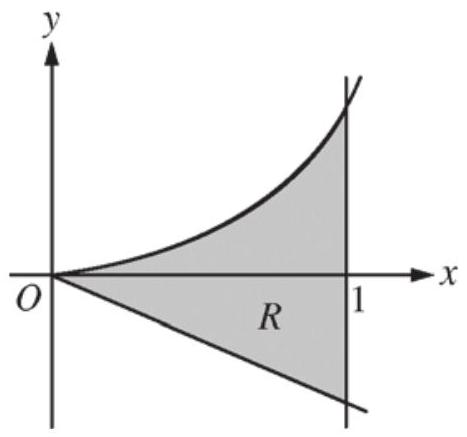
\includegraphics[width=0.6\linewidth]{figures/bc-2014_fig3.jpg}
\end{center}
Let $R$ be the shaded region bounded by the graph of $y=x e^{x^{2}}$, the line $y=-2 x$, and the vertical line $x=1$, as shown in the figure above.\\
\begin{parts}
\part Find the area of $R$.
\part Write, but do not evaluate, an integral expression that gives the volume of the solid generated when $R$ is rotated about the horizontal line $y=-2$.
\part Write, but do not evaluate, an expression involving one or more integrals that gives the perimeter of $R$.
\end{parts}
\begin{solution}
\begin{parts}
\part Area $=\int_{0}^{1}\left(x e^{x^{2}}-(-2 x)\right) d x$

\[\begin{aligned}
& =\left[\frac{1}{2} e^{x^{2}}+x^{2}\right]_{x=0}^{x=1} \\
& =\left(\frac{1}{2} e+1\right)-\frac{1}{2}=\frac{e+1}{2}
\end{aligned}\]
\part Volume $=\pi \int_{0}^{1}\left[\left(x e^{x^{2}}+2\right)^{2}-(-2 x+2)^{2}\right] d x$
\part $y^{\prime}=\frac{d}{d x}\left(x e^{x^{2}}\right)=e^{x^{2}}+2 x^{2} e^{x^{2}}=e^{x^{2}}\left(1+2 x^{2}\right)$

\[\text { Perimeter }=\sqrt{5}+2+e+\int_{0}^{1} \sqrt{1+\left[e^{x^{2}}\left(1+2 x^{2}\right)\right]^{2}} d x\]
\end{parts}
\par\medskip
\textbf{Rubric:}\par
\begin{parts}
\part $1: y^{\prime}=e^{x^{2}}\left(1+2 x^{2}\right)$
\end{parts}
\end{solution}

\question
% Q6 | 2014 Calculus BC | Part B | Calculator Prohibited
The Taylor series for a function $f$ about $x=1$ is given by $\sum_{n=1}^{\infty}(-1)^{n+1} \frac{2^{n}}{n}(x-1)^{n}$ and converges to $f(x)$ for $|x-1|<R$, where $R$ is the radius of convergence of the Taylor series.\\
\begin{parts}
\part Find the value of $R$.
\part Find the first three nonzero terms and the general term of the Taylor series for $f^{\prime}$, the derivative of $f$, about $x=1$.
\part The Taylor series for $f^{\prime}$ about $x=1$, found in part (b), is a geometric series. Find the function $f^{\prime}$ to which the series converges for $|x-1|<R$. Use this function to determine $f$ for $|x-1|<R$.
\end{parts}
\begin{solution}
\begin{parts}
\part Let $a_{n}$ be the $n$th term of the Taylor series.

\begin{align*}& 
\frac{a_{n+1}}{a_{n}} & =\frac{(-1)^{n+2} 2^{n+1}(x-1)^{n+1}}{n+1} \cdot \frac{n}{(-1)^{n+1} 2^{n}(x-1)^{n}} \\
& =\frac{-2 n(x-1)}{n+1}
 \\
& \lim _{n \rightarrow \infty}\left|\frac{-2 n(x-1)}{n+1}\right|=2|x-1| \\
& 2|x-1|<1 \Rightarrow|x-1|<\frac{1}{2}\end{align*}

The radius of convergence is $R=\frac{1}{2}$.
\part The first three nonzero terms are

\[2-4(x-1)+8(x-1)^{2}\]

The general term is $(-1)^{n+1} 2^{n}(x-1)^{n-1}$ for $n \geq 1$.
\part The common ratio is $-2(x-1)$.

\begin{align*}& f^{\prime}(x)=\frac{2}{1-(-2(x-1))}=\frac{2}{2 x-1} \text { for }|x-1|<\frac{1}{2} \\
& f(x)=\int \frac{2}{2 x-1} d x=\ln |2 x-1|+C \\
& f(1)=0 \\
& \ln |1|+C=0 \Rightarrow C=0 \\
& f(x)=\ln |2 x-1| \text { for }|x-1|<\frac{1}{2}\end{align*}
\end{parts}
\par\medskip
\textbf{Rubric:}\par
\begin{parts}
\part $3:\left\{\begin{array}{l}
1: \text { sets up ratio } \\
1: \text { computes limit of ratio } \\
1: \text { determines radius of convergence }
\end{array}\right.$
\part $3:\left\{\begin{array}{l}
2: \text { first three nonzero terms } \\
1: \text { general term }
\end{array}\right.$
\part $3:\left\{\begin{array}{l}
1: f^{\prime}(x) \\
1: \text { antiderivative } \\
1: f(x)
\end{array}\right.$
\end{parts}
\end{solution}

\end{questions}

\section*{2015 AP Calculus BC}

\begin{questions}

\question
% Q1 | 2015 Calculus BC | Part A | Calculator Active
The rate at which rainwater flows into a drainpipe is modeled by the function $R$, where $R(t)=20 \sin \left(\frac{t^{2}}{35}\right)$ cubic feet per hour, $t$ is measured in hours, and $0 \leq t \leq 8$. The pipe is partially blocked, allowing water to drain out the other end of the pipe at a rate modeled by $D(t)=-0.04 t^{3}+0.4 t^{2}+0.96 t$ cubic feet per hour, for $0 \leq t \leq 8$. There are 30 cubic feet of water in the pipe at time $t=0$.\\
\begin{parts}
\part How many cubic feet of rainwater flow into the pipe during the 8 -hour time interval $0 \leq t \leq 8$ ?
\part Is the amount of water in the pipe increasing or decreasing at time $t=3$ hours? Give a reason for your answer.
\part At what time $t, 0 \leq t \leq 8$, is the amount of water in the pipe at a minimum? Justify your answer.
\part The pipe can hold 50 cubic feet of water before overflowing. For $t>8$, water continues to flow into and out of the pipe at the given rates until the pipe begins to overflow. Write, but do not solve, an equation involving one or more integrals that gives the time $w$ when the pipe will begin to overflow.
\end{parts}
\begin{solution}
\begin{parts}
\part $\quad \int_{0}^{8} R(t) d t=76.570$
\part $\quad R(3)-D(3)=-0.313632<0$

Since $R(3)<D(3)$, the amount of water in the pipe is decreasing at time $t=3$ hours.
\part The amount of water in the pipe at time $t, 0 \leq t \leq 8$, is $30+\int_{0}^{t}[R(x)-D(x)] d x$.\\
$R(t)-D(t)=0 \Rightarrow t=0,3.271658$

\begin{center}
\begin{tabular}{c|c}
$t$ & Amount of water in the pipe \\
\hline
0 & 30 \\
3.271658 & 27.964561 \\
8 & 48.543686 \\
\end{tabular}
\end{center}

The amount of water in the pipe is a minimum at time $t=3.272$ (or 3.271) hours.
\part $30+\int_{0}^{w}[R(t)-D(t)] d t=50$
\end{parts}
\par\medskip
\textbf{Rubric:}\par
\begin{parts}
\part $2:\left\{\begin{array}{l}1: \text { integrand } \\ 1: \text { answer }\end{array}\right.$
\part $2:\left\{\begin{array}{l}1: \text { considers } R(3) \text { and } D(3) \\ 1: \text { answer and reason }\end{array}\right.$
\part $3:\left\{\begin{array}{l}1: \text { considers } \\ 1: \text { answer } \\ 1: \text { justification }\end{array}\right.$
\part $2:\left\{\begin{array}{l}1: \text { integral } \\ 1: \text { equation }\end{array}\right.$
\end{parts}
\end{solution}

\question
% Q2 | 2015 Calculus BC | Part A | Calculator Active
At time $t \geq 0$, a particle moving along a curve in the $x y$-plane has position $(x(t), y(t))$ with velocity vector $v(t)=\left(\cos \left(t^{2}\right), e^{0.5 t}\right)$. At $t=1$, the particle is at the point $(3,5)$.\\
\begin{parts}
\part Find the $x$-coordinate of the position of the particle at time $t=2$.
\part For $0<t<1$, there is a point on the curve at which the line tangent to the curve has a slope of 2 . At what time is the object at that point?
\part Find the time at which the speed of the particle is 3 .
\part Find the total distance traveled by the particle from time $t=0$ to time $t=1$.
\end{parts}
\begin{solution}
\begin{parts}
\part $\quad x(2)=3+\int_{1}^{2} \cos \left(t^{2}\right) d t=2.557$ (or 2.556)
\part $\frac{d y}{d x}=\frac{d y / d t}{d x / d t}=\frac{e^{0.5 t}}{\cos \left(t^{2}\right)}$

\[\begin{aligned}
& \frac{e^{0.5 t}}{\cos \left(t^{2}\right)}=2 \\
& t=0.840
\end{aligned}\]
\part Speed $=\sqrt{\cos ^{2}\left(t^{2}\right)+e^{t}}$

\[\begin{aligned}
& \sqrt{\cos ^{2}\left(t^{2}\right)+e^{t}}=3 \\
& t=2.196(\text { or } 2.195)
\end{aligned}\]
\part Distance $=\int_{0}^{1} \sqrt{\cos ^{2}\left(t^{2}\right)+e^{t}} d t=1.595$ (or 1.594)
\end{parts}
\par\medskip
\textbf{Rubric:}\par
\begin{parts}
\part $2:\left\{\begin{array}{l}
1: \text { integral } \\
1: \text { answer }
\end{array}\right.$
\end{parts}
\end{solution}

\question
% Q3 | 2015 Calculus BC | Part B | Calculator Prohibited
\begin{center}
\begin{tabular}{|c|c|c|c|c|c|}
\hline
\begin{tabular}{c}
$t$ \\
(minutes) \\
\end{tabular} & 0 & 12 & 20 & 24 & 40 \\
\hline
\begin{tabular}{c}
$v(t)$ \\
(meters per minute) \\
\end{tabular} & 0 & 200 & 240 & -220 & 150 \\
\hline
\end{tabular}
\end{center}
Johanna jogs along a straight path. For $0 \leq t \leq 40$, Johanna's velocity is given by a differentiable function $v$. Selected values of $v(t)$, where $t$ is measured in minutes and $v(t)$ is measured in meters per minute, are given in the table above.\\
\begin{parts}
\part Use the data in the table to estimate the value of $v^{\prime}(16)$.
\part Using correct units, explain the meaning of the definite integral $\int_{0}^{40}|v(t)| d t$ in the context of the problem. Approximate the value of $\int_{0}^{40}|v(t)| d t$ using a right Riemann sum with the four subintervals indicated in the table.
\part Bob is riding his bicycle along the same path. For $0 \leq t \leq 10$, Bob's velocity is modeled by $B(t)=t^{3}-6 t^{2}+300$, where $t$ is measured in minutes and $B(t)$ is measured in meters per minute. Find Bob's acceleration at time $t=5$.
\part Based on the model $B$ from part (c), find Bob's average velocity during the interval $0 \leq t \leq 10$.
\end{parts}
\begin{solution}
\begin{parts}
\part $v^{\prime}(16) \approx \frac{240-200}{20-12}=5$ meters $/ \mathrm{min}^{2}$
\part $\int_{0}^{40}|v(t)| d t$ is the total distance Johanna jogs, in meters, over the time interval $0 \leq t \leq 40$ minutes.

\begin{align*}\int_{0}^{40}|v(t)| d t & \approx 12 \cdot|v(12)|+8 \cdot|v(20)|+4 \cdot|v(24)|+16 \cdot|v(40)| \\
& =12 \cdot 200+8 \cdot 240+4 \cdot 220+16 \cdot 150 \\
& =2400+1920+880+2400 \\
& =7600 \text { meters }\end{align*}
\part Bob's acceleration is $B^{\prime}(t)=3 t^{2}-12 t$.

\[B^{\prime}(5)=3(25)-12(5)=15 \text { meters } / \mathrm{min}^{2}\]
\part Avg vel $=\frac{1}{10} \int_{0}^{10}\left(t^{3}-6 t^{2}+300\right) d t$

\[\begin{aligned}
& =\frac{1}{10}\left[\frac{t^{4}}{4}-2 t^{3}+300 t\right]_{0}^{10} \\
& =\frac{1}{10}\left[\frac{10000}{4}-2000+3000\right]=350 \text { meters } / \mathrm{min}
\end{aligned}\]
\end{parts}
\par\medskip
\textbf{Rubric:}\par
\begin{parts}
\part 1 : approximation
\part $3:\left\{\begin{array}{l}
1: \text { explanation } \\
1: \text { right Riemann sum } \\
1: \text { approximation }
\end{array}\right.$
\part $2:\left\{\begin{array}{l}1: \text { uses } B^{\prime}(t) \\ 1: \text { answer }\end{array}\right.$
\part $3:\left\{\begin{array}{l}1: \text { integral } \\ 1: \text { antiderivative } \\ 1: \text { answer }\end{array}\right.$
\end{parts}
\end{solution}

\question
% Q4 | 2015 Calculus BC | Part B | Calculator Prohibited
Consider the differential equation $\frac{d y}{d x}=2 x-y$.\\
\begin{parts}
\part On the axes provided, sketch a slope field for the given differential equation at the six points indicated.\\
\begin{center}
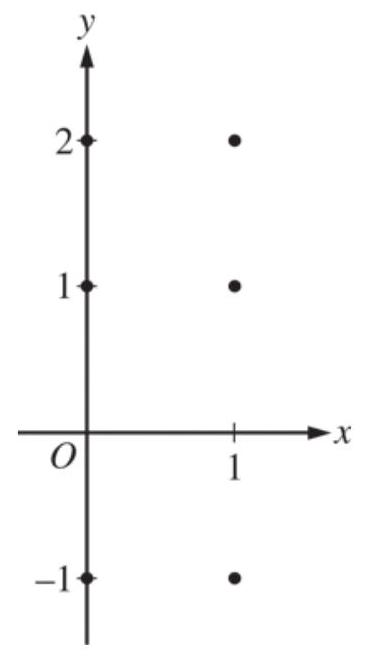
\includegraphics[width=0.6\linewidth]{figures/bc-2015_fig1.jpg}
\end{center}
\part Find $\frac{d^{2} y}{d x^{2}}$ in terms of $x$ and $y$. Determine the concavity of all solution curves for the given differential equation in Quadrant II. Give a reason for your answer.
\part Let $y=f(x)$ be the particular solution to the differential equation with the initial condition $f(2)=3$. Does $f$ have a relative minimum, a relative maximum, or neither at $x=2$ ? Justify your answer.
\part Find the values of the constants $m$ and $b$ for which $y=m x+b$ is a solution to the differential equation.
\end{parts}
\begin{solution}
(a)\\
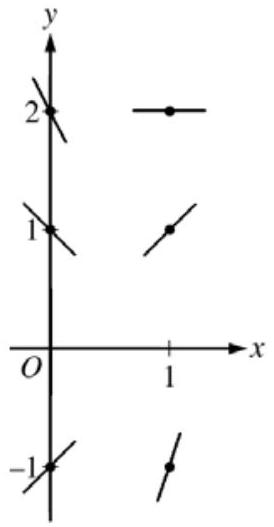
\includegraphics[width=0.6\linewidth]{figures/sg-bc-2015_fig1.jpg}\\
\begin{parts}
\part $\frac{d^{2} y}{d x^{2}}=2-\frac{d y}{d x}=2-(2 x-y)=2-2 x+y$

In Quadrant II, $x<0$ and $y>0$, so $2-2 x+y>0$.\\
Therefore, all solution curves are concave up in Quadrant II.
\part $\left.\frac{d y}{d x}\right|_{(x, y)=(2,3)}=2(2)-3=1 \neq 0$

Therefore, $f$ has neither a relative minimum nor a relative maximum at $x=2$.
\part $y=m x+b \Rightarrow \frac{d y}{d x}=\frac{d}{d x}(m x+b)=m$\\
$2 x-y=m$\\
$2 x-(m x+b)=m$\\
$(2-m) x-(m+b)=0$\\
$2-m=0 \Rightarrow m=2$\\
$b=-m \Rightarrow b=-2$

Therefore, $m=2$ and $b=-2$.
\end{parts}
\par\medskip
\textbf{Rubric:}\par
\begin{parts}
\part $2:\left\{\begin{array}{l}1: \text { slopes where } x=0 \\ 1: \text { slopes where } x=1\end{array}\right.$
\part $2:\left\{\begin{array}{l}1: \frac{d^{2} y}{d x^{2}} \\ 1: \text { concave up with reason }\end{array}\right.$
\part $2:\left\{\begin{array}{l}1: \text { considers }\left.\frac{d y}{d x}\right|_{(x, y)=(2,3)} \\ 1: \text { conclusion with justification }\end{array}\right.$
\part $3:\left\{\begin{array}{l}1: \frac{d}{d x}(m x+b)=m \\ 1: 2 x-y=m \\ 1: \text { answer }\end{array}\right.$
\end{parts}
\end{solution}

\question
% Q5 | 2015 Calculus BC | Part B | Calculator Prohibited
Consider the function $f(x)=\frac{1}{x^{2}-k x}$, where $k$ is a nonzero constant. The derivative of $f$ is given by $f^{\prime}(x)=\frac{k-2 x}{\left(x^{2}-k x\right)^{2}}$.\\
\begin{parts}
\part Let $k=3$, so that $f(x)=\frac{1}{x^{2}-3 x}$. Write an equation for the line tangent to the graph of $f$ at the point whose $x$-coordinate is 4 .
\part Let $k=4$, so that $f(x)=\frac{1}{x^{2}-4 x}$. Determine whether $f$ has a relative minimum, a relative maximum, or neither at $x=2$. Justify your answer.
\part Find the value of $k$ for which $f$ has a critical point at $x=-5$.
\part Let $k=6$, so that $f(x)=\frac{1}{x^{2}-6 x}$. Find the partial fraction decomposition for the function $f$.
Find $\int f(x) d x$.
\end{parts}
\begin{solution}
\begin{parts}
\part $f(4)=\frac{1}{4^{2}-3 \cdot 4}=\frac{1}{4} \quad f^{\prime}(4)=\frac{3-2 \cdot 4}{\left(4^{2}-3 \cdot 4\right)^{2}}=-\frac{5}{16}$

An equation for the line tangent to the graph of $f$ at the point whose $x$-coordinate is 4 is $y=-\frac{5}{16}(x-4)+\frac{1}{4}$.
\part $f^{\prime}(x)=\frac{4-2 x}{\left(x^{2}-4 x\right)^{2}} \quad f^{\prime}(2)=\frac{4-2 \cdot 2}{\left(2^{2}-4 \cdot 2\right)^{2}}=0 f^{\prime}(x)$ changes sign from positive to negative at $x=2$. Therefore, $f$ has a relative maximum at $x=2$.
\part $f^{\prime}(-5)=\frac{k-2 \cdot(-5)}{\left((-5)^{2}-k \cdot(-5)\right)^{2}}=0 \Rightarrow k=-10$
\part $\frac{1}{x^{2}-6 x}=\frac{1}{x(x-6)}=\frac{A}{x}+\frac{B}{x-6} \Rightarrow 1=A(x-6)+B x$

\[\begin{aligned}
& x=0 \Rightarrow 1=A \cdot(-6) \Rightarrow A=-\frac{1}{6} \\
& x=6 \Rightarrow 1=B \cdot(6) \Rightarrow B=\frac{1}{6} \\
& \begin{aligned}
\frac{1}{x(x-6)} & =\frac{-1 / 6}{x}+\frac{1 / 6}{x-6} \\
\int f(x) d x & =\int\left(\frac{-1 / 6}{x}+\frac{1 / 6}{x-6}\right) d x \\
& =-\frac{1}{6} \ln |x|+\frac{1}{6} \ln |x-6|+C=\frac{1}{6} \ln \left|\frac{x-6}{x}\right|+C
\end{aligned}
\end{aligned}\]
\end{parts}
\par\medskip
\textbf{Rubric:}\par
\begin{parts}
\part $2:\left\{\begin{array}{l}
1: \text { slope } \\
1: \text { tangent line equation }
\end{array}\right.$
\part $2:\left\{\begin{array}{l}
1: \text { considers } f^{\prime}(2) \\
1: \text { answer with justification }
\end{array}\right.$
\part 1 : answer
\part $4:\left\{\begin{array}{l}2: \text { partial fraction decomposition } \\ 2: \text { general antiderivative }\end{array}\right.$
\end{parts}
\end{solution}

\question
% Q6 | 2015 Calculus BC | Part B | Calculator Prohibited
The Maclaurin series for a function $f$ is given by $\sum_{n=1}^{\infty} \frac{(-3)^{n-1}}{n} x^{n}=x-\frac{3}{2} x^{2}+3 x^{3}-\cdots+\frac{(-3)^{n-1}}{n} x^{n}+\cdots$ and converges to $f(x)$ for $|x|<R$, where $R$ is the radius of convergence of the Maclaurin series.\\
\begin{parts}
\part Use the ratio test to find $R$.
\part Write the first four nonzero terms of the Maclaurin series for $f^{\prime}$, the derivative of $f$. Express $f^{\prime}$ as a rational function for $|x|<R$.
\part Write the first four nonzero terms of the Maclaurin series for $e^{x}$. Use the Maclaurin series for $e^{x}$ to write the third-degree Taylor polynomial for $g(x)=e^{x} f(x)$ about $x=0$.
\end{parts}
\begin{solution}
\begin{parts}
\part Let $a_{n}$ be the $n$th term of the Maclaurin series.

\begin{align*}& \frac{a_{n+1}}{a_{n}}=\frac{(-3)^{n} x^{n+1}}{n+1} \cdot \frac{n}{(-3)^{n-1} x^{n}}=\frac{-3 n}{n+1} \cdot x \\
& \lim _{n \rightarrow \infty}\left|\frac{-3 n}{n+1} \cdot x\right|=3|x| \\
& 3|x|<1 \Rightarrow|x|<\frac{1}{3}\end{align*}

The radius of convergence is $R=\frac{1}{3}$.
\part The first four nonzero terms of the Maclaurin series for $f^{\prime}$ are $1-3 x+9 x^{2}-27 x^{3}$.

\[f^{\prime}(x)=\frac{1}{1-(-3 x)}=\frac{1}{1+3 x}\]
\part The first four nonzero terms of the Maclaurin series for $e^{x}$ are $1+x+\frac{x^{2}}{2!}+\frac{x^{3}}{3!}$.

The product of the Maclaurin series for $e^{x}$ and the Maclaurin series for $f$ is

\[\begin{aligned}
& \left(1+x+\frac{x^{2}}{2!}+\frac{x^{3}}{3!}+\cdots\right)\left(x-\frac{3}{2} x^{2}+3 x^{3}-\cdots\right) \\
& \quad=x-\frac{1}{2} x^{2}+2 x^{3}+\cdots
\end{aligned}\]

The third-degree Taylor polynomial for $g(x)=e^{x} f(x)$ about $x=0$ is $T_{3}(x)=x-\frac{1}{2} x^{2}+2 x^{3}$.
\end{parts}
\par\medskip
\textbf{Rubric:}\par
\begin{parts}
\part $3:\left\{\begin{array}{l}
1: \text { sets up ratio } \\
1: \text { computes limit of ratio } \\
1: \text { determines radius of convergence }
\end{array}\right.$
\part $3:\left\{\begin{array}{l}
2: \text { first four nonzero terms } \\
1: \text { rational function }
\end{array}\right.$
\part $3:\left\{\begin{aligned}
1: & \text { first four nonzero terms } \\
& \text { of the Maclaurin series for } e^{x} \\
2: & \text { Taylor polynomial }
\end{aligned}\right.$
\end{parts}
\end{solution}

\end{questions}

\section*{2016 AP Calculus BC}

\begin{questions}

\question
% Q1 | 2016 Calculus BC | Part A | Calculator Active
\begin{center}
\begin{tabular}{|c||c|c|c|c|c|}
\hline
\begin{tabular}{c}
$t$ \\
(hours) \\
\end{tabular} & 0 & 1 & 3 & 6 & 8 \\
\hline
\begin{tabular}{c}
$R(t)$ \\
(liters / hour) \\
\end{tabular} & 1340 & 1190 & 950 & 740 & 700 \\
\hline
\end{tabular}
\end{center}
Water is pumped into a tank at a rate modeled by $W(t)=2000 e^{-t^{2} / 20}$ liters per hour for $0 \leq t \leq 8$, where $t$ is measured in hours. Water is removed from the tank at a rate modeled by $R(t)$ liters per hour, where $R$ is differentiable and decreasing on $0 \leq t \leq 8$. Selected values of $R(t)$ are shown in the table above. At time $t=0$, there are 50,000 liters of water in the tank.\\
\begin{parts}
\part Estimate $R^{\prime}(2)$. Show the work that leads to your answer. Indicate units of measure.
\part Use a left Riemann sum with the four subintervals indicated by the table to estimate the total amount of water removed from the tank during the 8 hours. Is this an overestimate or an underestimate of the total amount of water removed? Give a reason for your answer.
\part Use your answer from part (b) to find an estimate of the total amount of water in the tank, to the nearest liter, at the end of 8 hours.
\part For $0 \leq t \leq 8$, is there a time $t$ when the rate at which water is pumped into the tank is the same as the rate at which water is removed from the tank? Explain why or why not.
\end{parts}
\begin{solution}
\begin{parts}
\part $\quad R^{\prime}(2) \approx \frac{R(3)-R(1)}{3-1}=\frac{950-1190}{3-1}=-120$ liters $/ \mathrm{hr}^{2}$
\part The total amount of water removed is given by $\int_{0}^{8} R(t) d t$.

\begin{align*}\int_{0}^{8} R(t) d t & \approx 1 \cdot R(0)+2 \cdot R(1)+3 \cdot R(3)+2 \cdot R(6) \\
& =1(1340)+2(1190)+3(950)+2(740) \\
& =8050 \text { liters }\end{align*}

This is an overestimate since $R$ is a decreasing function.
\part Total $\approx 50000+\int_{0}^{8} W(t) d t-8050$

\[=50000+7836.195325-8050 \approx 49786 \text { liters }\]
\part $W(0)-R(0)>0, W(8)-R(8)<0$, and $W(t)-R(t)$ is continuous.

Therefore, the Intermediate Value Theorem guarantees at least one time $t, 0<t<8$, for which $W(t)-R(t)=0$, or $W(t)=R(t)$.

For this value of $t$, the rate at which water is pumped into the tank is the same as the rate at which water is removed from the tank.
\end{parts}
\par\medskip
\textbf{Rubric:}\par
\begin{parts}
\part $2:\left\{\begin{array}{l}1: \text { estimate } \\ 1: \text { units }\end{array}\right.$
\part $3:\left\{\begin{array}{l}1: \text { left Riemann sum } \\ 1: \text { estimate } \\ 1: \text { overestimate with reason }\end{array}\right.$
\part $2:\left\{\begin{array}{l}1: \text { integral } \\ 1: \text { estimate }\end{array}\right.$
\part $2:\left\{\begin{array}{l}1: \text { considers } W(t)-R(t) \\ 1: \text { answer with explanation }\end{array}\right.$
\end{parts}
\end{solution}

\question
% Q2 | 2016 Calculus BC | Part A | Calculator Active
\begin{center}
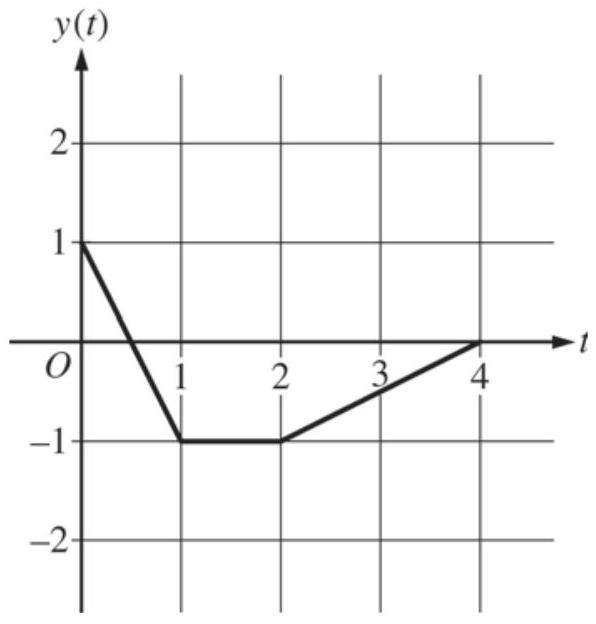
\includegraphics[width=0.6\linewidth]{figures/bc-2016_fig1.jpg}
\end{center}
At time $t$, the position of a particle moving in the $x y$-plane is given by the parametric functions $(x(t), y(t))$, where $\frac{d x}{d t}=t^{2}+\sin \left(3 t^{2}\right)$. The graph of $y$, consisting of three line segments, is shown in the figure above. At $t=0$, the particle is at position $(5,1)$.\\
\begin{parts}
\part Find the position of the particle at $t=3$.
\part Find the slope of the line tangent to the path of the particle at $t=3$.
\part Find the speed of the particle at $t=3$.
\part Find the total distance traveled by the particle from $t=0$ to $t=2$.
\end{parts}
\begin{solution}
\begin{parts}
\part $x(3)=x(0)+\int_{0}^{3} x^{\prime}(t) d t=5+9.377035=14.377$

\[y(3)=-\frac{1}{2}\]

The position of the particle at $t=3$ is $(14.377,-0.5)$.
\part Slope $=\frac{y^{\prime}(3)}{x^{\prime}(3)}=\frac{0.5}{9.956376}=0.05$
\part Speed $=\sqrt{\left(x^{\prime}(3)\right)^{2}+\left(y^{\prime}(3)\right)^{2}}=9.969$ (or 9.968)
\part Distance $=\int_{0}^{2} \sqrt{\left(x^{\prime}(t)\right)^{2}+\left(y^{\prime}(t)\right)^{2}} d t$

\[\begin{aligned}
& =\int_{0}^{1} \sqrt{\left(x^{\prime}(t)\right)^{2}+(-2)^{2}} d t+\int_{1}^{2} \sqrt{\left(x^{\prime}(t)\right)^{2}+0^{2}} d t \\
& =2.237871+2.112003=4.350(\text { or } 4.349)
\end{aligned}\]
\end{parts}
\par\medskip
\textbf{Rubric:}\par
\begin{parts}
\part $3:\left\{\begin{array}{l}
1: \text { integral } \\
1: \text { uses initial condition } \\
1: \text { answer }
\end{array}\right.$
\part 1 : slope
\part $2:\left\{\begin{array}{l}
1: \text { expression for speed } \\
1: \text { answer }
\end{array}\right.$
\part $3:\left\{\begin{array}{l}1: \text { expression for distance } \\ 1: \text { integrals } \\ 1: \text { answer }\end{array}\right.$
\end{parts}
\end{solution}

\question
% Q3 | 2016 Calculus BC | Part B | Calculator Prohibited
\begin{center}
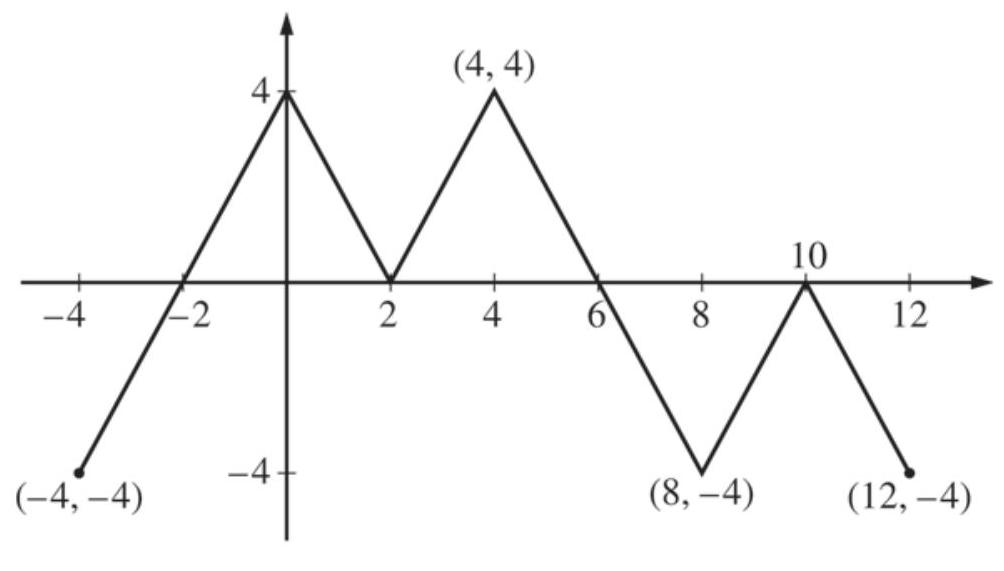
\includegraphics[width=0.6\linewidth]{figures/bc-2016_fig2.jpg}
\end{center}

Graph of $f$\\
The figure above shows the graph of the piecewise-linear function $f$. For $-4 \leq x \leq 12$, the function $g$ is defined by $g(x)=\int_{2}^{x} f(t) d t$.\\
\begin{parts}
\part Does $g$ have a relative minimum, a relative maximum, or neither at $x=10$ ? Justify your answer.
\part Does the graph of $g$ have a point of inflection at $x=4$ ? Justify your answer.
\part Find the absolute minimum value and the absolute maximum value of $g$ on the interval $-4 \leq x \leq 12$. Justify your answers.
\part For $-4 \leq x \leq 12$, find all intervals for which $g(x) \leq 0$.
\end{parts}
\begin{solution}
\begin{parts}
\part The function $g$ has neither a relative minimum nor a relative maximum at $x=10$ since $g^{\prime}(x)=f(x)$ and $f(x) \leq 0$ for $8 \leq x \leq 12$.
\part The graph of $g$ has a point of inflection at $x=4$ since $g^{\prime}(x)=f(x)$ is increasing for $2 \leq x \leq 4$ and decreasing for $4 \leq x \leq 8$.
\part $g^{\prime}(x)=f(x)$ changes sign only at $x=-2$ and $x=6$.

\begin{center}
\begin{tabular}{r|r}
\multicolumn{1}{c|}{$x$} & $g(x)$ \\
\hline
-4 & -4 \\
-2 & -8 \\
6 & 8 \\
12 & -4 \\
\end{tabular}
\end{center}

On the interval $-4 \leq x \leq 12$, the absolute minimum value is $g(-2)=-8$ and the absolute maximum value is $g(6)=8$.
\part $g(x) \leq 0$ for $-4 \leq x \leq 2$ and $10 \leq x \leq 12$.
\end{parts}
\par\medskip
\textbf{Rubric:}\par
\begin{parts}
\part 1 : answer with justification
\part 1 : answer with justification
\part $4:\left\{\begin{aligned} 1: & \text { considers } x=-2 \text { and } x=6 \\ & \text { as candidates } \\ 1: & \text { considers } x=-4 \text { and } x=12 \\ 2: & \text { answers with justification }\end{aligned}\right.$
\part 2 : intervals
\end{parts}
\end{solution}

\question
% Q4 | 2016 Calculus BC | Part B | Calculator Prohibited
Consider the differential equation $\frac{d y}{d x}=x^{2}-\frac{1}{2} y$.\\
\begin{parts}
\part Find $\frac{d^{2} y}{d x^{2}}$ in terms of $x$ and $y$.
\part Let $y=f(x)$ be the particular solution to the given differential equation whose graph passes through the point $(-2,8)$. Does the graph of $f$ have a relative minimum, a relative maximum, or neither at the point $(-2,8)$ ? Justify your answer.
\part Let $y=g(x)$ be the particular solution to the given differential equation with $g(-1)=2$. Find $\lim _{x \rightarrow-1}\left(\frac{g(x)-2}{3(x+1)^{2}}\right)$. Show the work that leads to your answer.
\part Let $y=h(x)$ be the particular solution to the given differential equation with $h(0)=2$. Use Euler's method, starting at $x=0$ with two steps of equal size, to approximate $h(1)$.
\end{parts}
\begin{solution}
\begin{parts}
\part $\frac{d^{2} y}{d x^{2}}=2 x-\frac{1}{2} \frac{d y}{d x}=2 x-\frac{1}{2}\left(x^{2}-\frac{1}{2} y\right)$
\part $\left.\frac{d y}{d x}\right|_{(x, y)=(-2,8)}=(-2)^{2}-\frac{1}{2} \cdot 8=0$

\[\left.\frac{d^{2} y}{d x^{2}}\right|_{(x, y)=(-2,8)}=2(-2)-\frac{1}{2}\left((-2)^{2}-\frac{1}{2} \cdot 8\right)=-4<0\]

Thus, the graph of $f$ has a relative maximum at the point $(-2,8)$.
\part $\lim _{x \rightarrow-1}(g(x)-2)=0$ and $\lim _{x \rightarrow-1} 3(x+1)^{2}=0$

Using L'Hospital's Rule,

\[\lim _{x \rightarrow-1}\left(\frac{g(x)-2}{3(x+1)^{2}}\right)=\lim _{x \rightarrow-1}\left(\frac{g^{\prime}(x)}{6(x+1)}\right)\]

\[\lim _{x \rightarrow-1} g^{\prime}(x)=0 \text { and } \lim _{x \rightarrow-1} 6(x+1)=0\]

Using L'Hospital's Rule,

\[\lim _{x \rightarrow-1}\left(\frac{g^{\prime}(x)}{6(x+1)}\right)=\lim _{x \rightarrow-1}\left(\frac{g^{\prime \prime}(x)}{6}\right)=\frac{-2}{6}=-\frac{1}{3}\]
\part $h\left(\frac{1}{2}\right) \approx h(0)+h^{\prime}(0) \cdot \frac{1}{2}=2+(-1) \cdot \frac{1}{2}=\frac{3}{2}$

\[h(1) \approx h\left(\frac{1}{2}\right)+h^{\prime}\left(\frac{1}{2}\right) \cdot \frac{1}{2} \approx \frac{3}{2}+\left(-\frac{1}{2}\right) \cdot \frac{1}{2}=\frac{5}{4}\]

2 : $\frac{d^{2} y}{d x^{2}}$ in terms of $x$ and $y$
\end{parts}
\par\medskip
\textbf{Rubric:}\par
\begin{parts}
\part 2 : conclusion with justification
\part $3:\left\{\begin{array}{l}2: \text { L'Hospital's Rule } \\ 1: \text { answer }\end{array}\right.$
\part $2:\left\{\begin{array}{l}1: \text { Euler's method } \\ 1: \text { approximation }\end{array}\right.$
\end{parts}
\end{solution}

\question
% Q5 | 2016 Calculus BC | Part B | Calculator Prohibited
\begin{center}
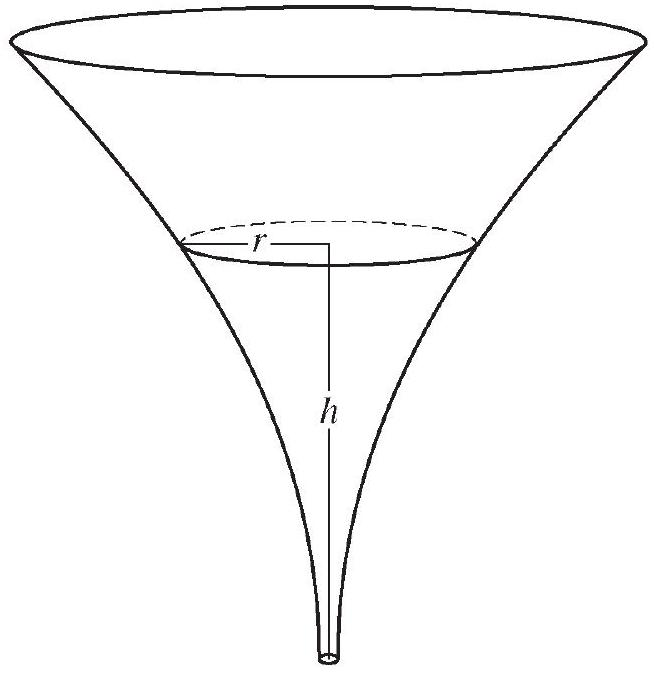
\includegraphics[width=0.6\linewidth]{figures/bc-2016_fig3.jpg}
\end{center}
The inside of a funnel of height 10 inches has circular cross sections, as shown in the figure above. At height $h$, the radius of the funnel is given by $r=\frac{1}{20}\left(3+h^{2}\right)$, where $0 \leq h \leq 10$. The units of $r$ and $h$ are inches.\\
\begin{parts}
\part Find the average value of the radius of the funnel.
\part Find the volume of the funnel.
\part The funnel contains liquid that is draining from the bottom. At the instant when the height of the liquid is $h=3$ inches, the radius of the surface of the liquid is decreasing at a rate of $\frac{1}{5}$ inch per second. At this instant, what is the rate of change of the height of the liquid with respect to time?
\end{parts}
\begin{solution}
\begin{parts}
\part Average radius $=\frac{1}{10} \int_{0}^{10} \frac{1}{20}\left(3+h^{2}\right) d h=\frac{1}{200}\left[3 h+\frac{h^{3}}{3}\right]_{0}^{10}$

\[=\frac{1}{200}\left(\left(30+\frac{1000}{3}\right)-0\right)=\frac{109}{60} \text { in }\]
\part Volume $=\pi \int_{0}^{10}\left(\left(\frac{1}{20}\right)\left(3+h^{2}\right)\right)^{2} d h=\frac{\pi}{400} \int_{0}^{10}\left(9+6 h^{2}+h^{4}\right) d h$

\[\begin{aligned}
& =\frac{\pi}{400}\left[9 h+2 h^{3}+\frac{h^{5}}{5}\right]_{0}^{10} \\
& =\frac{\pi}{400}\left(\left(90+2000+\frac{100000}{5}\right)-0\right)=\frac{2209 \pi}{40} \mathrm{in}^{3}
\end{aligned}\]
\part $\frac{d r}{d t}=\frac{1}{20}(2 h) \frac{d h}{d t}$

\[-\frac{1}{5}=\frac{3}{10} \frac{d h}{d t}\]

$\frac{d h}{d t}=-\frac{1}{5} \cdot \frac{10}{3}=-\frac{2}{3} \mathrm{in} / \mathrm{sec}$
\end{parts}
\par\medskip
\textbf{Rubric:}\par
\begin{parts}
\part $3:\left\{\begin{array}{l}1: \text { integral } \\ 1: \text { antiderivative } \\ 1: \text { answer }\end{array}\right.$
\part $3:\left\{\begin{array}{l}1: \text { integrand } \\ 1: \text { antiderivative } \\ 1: \text { answer }\end{array}\right.$
\part $3:\left\{\begin{array}{l}2: \text { chain rule } \\ 1: \text { answer }\end{array}\right.$
\end{parts}
\end{solution}

\question
% Q6 | 2016 Calculus BC | Part B | Calculator Prohibited
The function $f$ has a Taylor series about $x=1$ that converges to $f(x)$ for all $x$ in the interval of convergence. It is known that $f(1)=1, f^{\prime}(1)=-\frac{1}{2}$, and the $n$th derivative of $f$ at $x=1$ is given by $f^{(n)}(1)=(-1)^{n} \frac{(n-1)!}{2^{n}}$ for $n \geq 2$.\\
\begin{parts}
\part Write the first four nonzero terms and the general term of the Taylor series for $f$ about $x=1$.
\part The Taylor series for $f$ about $x=1$ has a radius of convergence of 2 . Find the interval of convergence. Show the work that leads to your answer.
\part The Taylor series for $f$ about $x=1$ can be used to represent $f(1.2)$ as an alternating series. Use the first three nonzero terms of the alternating series to approximate $f(1.2)$.
\part Show that the approximation found in part (c) is within 0.001 of the exact value of $f(1.2)$.
\end{parts}
\begin{solution}
\begin{parts}
\part $f(1)=1, f^{\prime}(1)=-\frac{1}{2}, f^{\prime \prime}(1)=\frac{1}{2^{2}}, f^{\prime \prime \prime}(1)=-\frac{2}{2^{3}}$

\begin{align*}f(x)=1 & -\frac{1}{2}(x-1)+\frac{1}{2^{2} \cdot 2}(x-1)^{2}-\frac{1}{2^{3} \cdot 3}(x-1)^{3}+\cdots \\
& +\frac{(-1)^{n}}{2^{n} \cdot n}(x-1)^{n}+\cdots\end{align*}
\part $\quad R=2$. The series converges on the interval $(-1,3)$.

When $x=-1$, the series is $1+1+\frac{1}{2}+\frac{1}{3}+\frac{1}{4}+\cdots$.\\
Since the harmonic series diverges, this series diverges.\\
When $x=3$, the series is $1-1+\frac{1}{2}-\frac{1}{3}+\frac{1}{4}+\cdots$.\\
Since the alternating harmonic series converges, this series converges.

Therefore, the interval of convergence is $-1<x \leq 3$.
\part $f(1.2) \approx 1-\frac{1}{2}(0.2)+\frac{1}{8}(0.2)^{2}=1-0.1+0.005=0.905$
\part The series for $f(1.2)$ alternates with terms that decrease in magnitude to 0 .

\[\left|f(1.2)-T_{2}(1.2)\right| \leq\left|\frac{-1}{2^{3} \cdot 3}(0.2)^{3}\right|=\frac{1}{3000} \leq 0.001\]
\end{parts}
\par\medskip
\textbf{Rubric:}\par
\begin{parts}
\part $4:\left\{\begin{array}{l}1: \text { first two terms } \\ 1: \text { third term } \\ 1: \text { fourth term } \\ 1: \text { general term }\end{array}\right.$
\part $2:\left\{\begin{array}{l}1: \text { identifies both endpoints } \\ 1: \text { analysis and interval of convergence }\end{array}\right.$
\part 1 : approximation
\part $2:\left\{\begin{array}{l}1: \text { error form } \\ 1: \text { analysis }\end{array}\right.$
\end{parts}
\end{solution}

\end{questions}

\section*{2017 AP Calculus BC}

\begin{questions}

\question
% Q1 | 2017 Calculus BC | Part A | Calculator Active
\begin{center}
\begin{tabular}{|c||c|c|c|c|}
\hline
\begin{tabular}{c}
$h$ \\
(feet) \\
\end{tabular} & 0 & 2 & 5 & 10 \\
\hline
\begin{tabular}{c}
$A(h)$ \\
(square feet) \\
\end{tabular} & 50.3 & 14.4 & 6.5 & 2.9 \\
\hline
\end{tabular}
\end{center}
A tank has a height of 10 feet. The area of the horizontal cross section of the tank at height $h$ feet is given by the function $A$, where $A(h)$ is measured in square feet. The function $A$ is continuous and decreases as $h$ increases. Selected values for $A(h)$ are given in the table above.\\
\begin{parts}
\part Use a left Riemann sum with the three subintervals indicated by the data in the table to approximate the volume of the tank. Indicate units of measure.
\part Does the approximation in part (a) overestimate or underestimate the volume of the tank? Explain your reasoning.
\part The area, in square feet, of the horizontal cross section at height $h$ feet is modeled by the function $f$ given by $f(h)=\frac{50.3}{e^{0.2 h}+h}$. Based on this model, find the volume of the tank. Indicate units of measure.
\part Water is pumped into the tank. When the height of the water is 5 feet, the height is increasing at the rate of 0.26 foot per minute. Using the model from part (c), find the rate at which the volume of water is changing with respect to time when the height of the water is 5 feet. Indicate units of measure.
\end{parts}
\begin{solution}
\begin{parts}
\part Volume $=\int_{0}^{10} A(h) d h$

\begin{align*}& \approx(2-0) \cdot A(0)+(5-2) \cdot A(2)+(10-5) \cdot A(5) \\
& =2 \cdot 50.3+3 \cdot 14.4+5 \cdot 6.5 \\
& =176.3 \text { cubic feet }\end{align*}
\part The approximation in part (a) is an overestimate because a left Riemann sum is used and $A$ is decreasing.
\part $\int_{0}^{10} f(h) d h=101.325338$

The volume is 101.325 cubic feet.
\part Using the model, $V(h)=\int_{0}^{h} f(x) d x$.

\[\begin{aligned}
\left.\frac{d V}{d t}\right|_{h=5} & =\left[\frac{d V}{d h} \cdot \frac{d h}{d t}\right]_{h=5} \\
& =\left[f(h) \cdot \frac{d h}{d t}\right]_{h=5} \\
& =f(5) \cdot 0.26=1.694419
\end{aligned}\]

When $h=5$, the volume of water is changing at a rate of
\end{parts}
\par\medskip
\textbf{Rubric:}\par
\begin{parts}
\part 1 : units in parts (a), (c), and (d)
\part $2:\left\{\begin{array}{l}1: \text { left Riemann sum } \\ 1: \text { approximation }\end{array}\right.$
\part 1 : overestimate with reason
\part $2:\left\{\begin{array}{l}1: \text { integral } \\ 1: \text { answer }\end{array}\right.$
\part $3:\left\{\begin{array}{l}2: \frac{d V}{d t} \\ 1: \text { answer }\end{array}\right.$
\end{parts}
\end{solution}

\question
% Q2 | 2017 Calculus BC | Part A | Calculator Active
\begin{center}
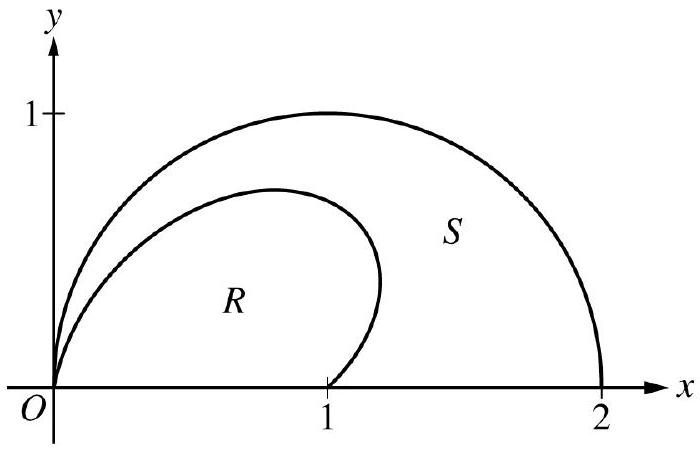
\includegraphics[width=0.6\linewidth]{figures/bc-2017_fig1.jpg}
\end{center}
The figure above shows the polar curves $r=f(\theta)=1+\sin \theta \cos (2 \theta)$ and $r=g(\theta)=2 \cos \theta$ for $0 \leq \theta \leq \frac{\pi}{2}$. Let $R$ be the region in the first quadrant bounded by the curve $r=f(\theta)$ and the $x$-axis. Let $S$ be the region in the first quadrant bounded by the curve $r=f(\theta)$, the curve $r=g(\theta)$, and the $x$-axis.\\
\begin{parts}
\part Find the area of $R$.
\part The ray $\theta=k$, where $0<k<\frac{\pi}{2}$, divides $S$ into two regions of equal area. Write, but do not solve, an equation involving one or more integrals whose solution gives the value of $k$.
\part For each $\theta, 0 \leq \theta \leq \frac{\pi}{2}$, let $w(\theta)$ be the distance between the points with polar coordinates $(f(\theta), \theta)$ and $(g(\theta), \theta)$. Write an expression for $w(\theta)$. Find $w_{A}$, the average value of $w(\theta)$ over the interval $0 \leq \theta \leq \frac{\pi}{2}$.
\part Using the information from part (c), find the value of $\boldsymbol{\theta}$ for which $w(\boldsymbol{\theta})=w_{A}$. Is the function $w(\boldsymbol{\theta})$ increasing or decreasing at that value of $\theta$ ? Give a reason for your answer.
\end{parts}
\begin{solution}
\begin{parts}
\part $\frac{1}{2} \int_{0}^{\pi / 2}(f(\theta))^{2} d \theta=0.648414$

The area of $R$ is 0.648 .
\part $\int_{0}^{k}\left((g(\theta))^{2}-(f(\theta))^{2}\right) d \theta=\frac{1}{2} \int_{0}^{\pi / 2}\left((g(\theta))^{2}-(f(\theta))^{2}\right) d \theta$\\
— OR —\\
$\int_{0}^{k}\left((g(\theta))^{2}-(f(\theta))^{2}\right) d \theta=\int_{k}^{\pi / 2}\left((g(\theta))^{2}-(f(\theta))^{2}\right) d \theta$
\part $w(\theta)=g(\theta)-f(\theta)$\\
$w_{A}=\frac{\int_{0}^{\pi / 2} w(\theta) d \theta}{\frac{\pi}{2}-0}=0.485446$

The average value of $w(\theta)$ on the interval $\left[0, \frac{\pi}{2}\right]$ is 0.485 .
\part $w(\theta)=w_{A}$ for $0 \leq \theta \leq \frac{\pi}{2} \Rightarrow \theta=0.517688$\\
$w(\theta)=w_{A}$ at $\theta=0.518$ (or 0.517).
\end{parts}
\par\medskip
\textbf{Rubric:}\par
\begin{parts}
\part $2:\left\{\begin{array}{l}
1: \text { integral } \\
1: \text { answer }
\end{array}\right.$
\part $2:\left\{\begin{aligned} 1: & \text { integral expression } \\ & \text { for one region } \\ 1: & \text { equation }\end{aligned}\right.$
\part $3:\left\{\begin{array}{l}1: w(\theta) \\ 1: \text { integral } \\ 1: \text { average value }\end{array}\right.$
\part $2:\left\{\begin{array}{l}1: \text { solves } w(\theta)=w_{A} \\ 1: \text { answer with reason }\end{array}\right.$
\end{parts}
\end{solution}

\question
% Q3 | 2017 Calculus BC | Part B | Calculator Prohibited
\begin{center}
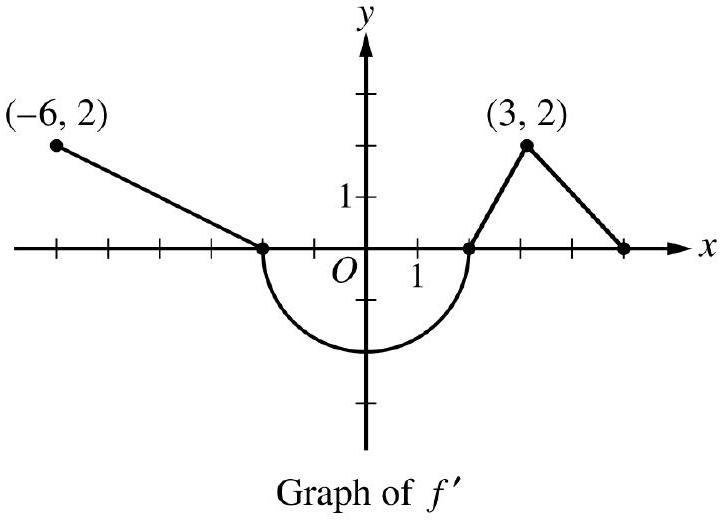
\includegraphics[width=0.6\linewidth]{figures/bc-2017_fig2.jpg}
\end{center}
The function $f$ is differentiable on the closed interval $[-6,5]$ and satisfies $f(-2)=7$. The graph of $f^{\prime}$, the derivative of $f$, consists of a semicircle and three line segments, as shown in the figure above.\\
\begin{parts}
\part Find the values of $f(-6)$ and $f(5)$.
\part On what intervals is $f$ increasing? Justify your answer.
\part Find the absolute minimum value of $f$ on the closed interval $[-6,5]$. Justify your answer.
\part For each of $f^{\prime \prime}(-5)$ and $f^{\prime \prime}(3)$, find the value or explain why it does not exist.
\end{parts}
\begin{solution}
\begin{parts}
\part $f(-6)=f(-2)+\int_{-2}^{-6} f^{\prime}(x) d x=7-\int_{-6}^{-2} f^{\prime}(x) d x=7-4=3$\\
$f(5)=f(-2)+\int_{-2}^{5} f^{\prime}(x) d x=7-2 \pi+3=10-2 \pi$
\part $f^{\prime}(x)>0$ on the intervals $[-6,-2)$ and $(2,5)$.

Therefore, $f$ is increasing on the intervals $[-6,-2]$ and $[2,5]$.
\part The absolute minimum will occur at a critical point where $f^{\prime}(x)=0$ or at an endpoint.\\
$f^{\prime}(x)=0 \Rightarrow x=-2, x=2$

\begin{center}
\begin{tabular}{c|c}
$x$ & $f(x)$ \\
\hline
-6 & 3 \\
-2 & 7 \\
2 & $7-2 \pi$ \\
5 & $10-2 \pi$ \\
\end{tabular}
\end{center}

The absolute minimum value is $f(2)=7-2 \pi$.
\part $f^{\prime \prime}(-5)=\frac{2-0}{-6-(-2)}=-\frac{1}{2}$\\
$\lim _{x \rightarrow 3^{-}} \frac{f^{\prime}(x)-f^{\prime}(3)}{x-3}=2$ and $\lim _{x \rightarrow 3^{+}} \frac{f^{\prime}(x)-f^{\prime}(3)}{x-3}=-1$\\
$f^{\prime \prime}(3)$ does not exist because\\
$\lim _{x \rightarrow 3^{-}} \frac{f^{\prime}(x)-f^{\prime}(3)}{x-3} \neq \lim _{x \rightarrow 3^{+}} \frac{f^{\prime}(x)-f^{\prime}(3)}{x-3}$.
\end{parts}
\par\medskip
\textbf{Rubric:}\par
\begin{parts}
\part $3:\left\{\begin{array}{l}1: \text { uses initial condition } \\ 1: f(-6) \\ 1: f(5)\end{array}\right.$
\part 2 : answer with justification
\part $2:\left\{\begin{array}{l}1: \text { considers } x=2 \\ 1: \text { answer with justification }\end{array}\right.$
\part $2:\left\{\begin{array}{c}1: f^{\prime \prime}(-5) \\ 1: f^{\prime \prime}(3) \text { does not exist } \\ \quad \text { with explanation }\end{array}\right.$
\end{parts}
\end{solution}

\question
% Q4 | 2017 Calculus BC | Part B | Calculator Prohibited
At time $t=0$, a boiled potato is taken from a pot on a stove and left to cool in a kitchen. The internal temperature of the potato is 91 degrees Celsius $\left({ }^{\circ} \mathrm{C}\right)$ at time $t=0$, and the internal temperature of the potato is greater than $27^{\circ} \mathrm{C}$ for all times $t>0$. The internal temperature of the potato at time $t$ minutes can be modeled by the function $H$ that satisfies the differential equation $\frac{d H}{d t}=-\frac{1}{4}(H-27)$, where $H(t)$ is measured in degrees Celsius and $H(0)=91$.\\
\begin{parts}
\part Write an equation for the line tangent to the graph of $H$ at $t=0$. Use this equation to approximate the internal temperature of the potato at time $t=3$.
\part Use $\frac{d^{2} H}{d t^{2}}$ to determine whether your answer in part (a) is an underestimate or an overestimate of the internal temperature of the potato at time $t=3$.
\part For $t<10$, an alternate model for the internal temperature of the potato at time $t$ minutes is the function $G$ that satisfies the differential equation $\frac{d G}{d t}=-(G-27)^{2 / 3}$, where $G(t)$ is measured in degrees Celsius and $G(0)=91$. Find an expression for $G(t)$. Based on this model, what is the internal temperature of the potato at time $t=3$ ?
\end{parts}
\begin{solution}
\begin{parts}
\part $H^{\prime}(0)=-\frac{1}{4}(91-27)=-16$\\
$H(0)=91$

An equation for the tangent line is $y=91-16 t$.

The internal temperature of the potato at time $t=3$ minutes is approximately $91-16 \cdot 3=43$ degrees Celsius.
\part $\frac{d^{2} H}{d t^{2}}=-\frac{1}{4} \frac{d H}{d t}=\left(-\frac{1}{4}\right)\left(-\frac{1}{4}\right)(H-27)=\frac{1}{16}(H-27)$\\
$H>27$ for $t>0 \Rightarrow \frac{d^{2} H}{d t^{2}}=\frac{1}{16}(H-27)>0$ for $t>0$\\
Therefore, the graph of $H$ is concave up for $t>0$. Thus, the answer in part (a) is an underestimate.
\part $\frac{d G}{(G-27)^{2 / 3}}=-d t$\\
$\int \frac{d G}{(G-27)^{2 / 3}}=\int(-1) d t$\\
$3(G-27)^{1 / 3}=-t+C$\\
$3(91-27)^{1 / 3}=0+C \Rightarrow C=12$\\
$3(G-27)^{1 / 3}=12-t$\\
$G(t)=27+\left(\frac{12-t}{3}\right)^{3}$ for $0 \leq t<10$

The internal temperature of the potato at time $t=3$ minutes is $27+\left(\frac{12-3}{3}\right)^{3}=54$ degrees Celsius.
\end{parts}
\par\medskip
\textbf{Rubric:}\par
\begin{parts}
\part $3:\left\{\begin{array}{l}1: \text { slope } \\ 1: \text { tangent line } \\ 1: \text { approximation }\end{array}\right.$
\part 1 : underestimate with reason
\part $5:\left\{\begin{array}{l}1: \text { separation of variables } \\ 1: \text { antiderivatives } \\ 1: \text { constant of integration and } \\ \quad \text { uses initial condition } \\ 1: \text { equation involving } G \text { and } t \\ 1: G(t) \text { and } G(3)\end{array}\right.$
\part Note: $\max 2 / 5[1-1-0-0-0]$ if no constant of integration
\part Note: $0 / 5$ if no separation of variables
\end{parts}
\end{solution}

\question
% Q5 | 2017 Calculus BC | Part B | Calculator Prohibited
Let $f$ be the function defined by $f(x)=\frac{3}{2 x^{2}-7 x+5}$.\\
\begin{parts}
\part Find the slope of the line tangent to the graph of $f$ at $x=3$.
\part Find the $x$-coordinate of each critical point of $f$ in the interval $1<x<2.5$. Classify each critical point as the location of a relative minimum, a relative maximum, or neither. Justify your answers.
\part Using the identity that $\frac{3}{2 x^{2}-7 x+5}=\frac{2}{2 x-5}-\frac{1}{x-1}$, evaluate $\int_{5}^{\infty} f(x) d x$ or show that the integral diverges.
\part Determine whether the series $\sum_{n=5}^{\infty} \frac{3}{2 n^{2}-7 n+5}$ converges or diverges. State the conditions of the test used for determining convergence or divergence.
\end{parts}
\begin{solution}
\begin{parts}
\part $f^{\prime}(x)=\frac{-3(4 x-7)}{\left(2 x^{2}-7 x+5\right)^{2}}$\\
$f^{\prime}(3)=\frac{(-3)(5)}{(18-21+5)^{2}}=-\frac{15}{4}$
\part $f^{\prime}(x)=\frac{-3(4 x-7)}{\left(2 x^{2}-7 x+5\right)^{2}}=0 \Rightarrow x=\frac{7}{4}$

The only critical point in the interval $1<x<2.5$ has $x$-coordinate $\frac{7}{4}$.\\
$f^{\prime}$ changes sign from positive to negative at $x=\frac{7}{4}$.\\
Therefore, $f$ has a relative maximum at $x=\frac{7}{4}$.
\part $\int_{5}^{\infty} f(x) d x=\lim _{b \rightarrow \infty} \int_{5}^{b} \frac{3}{2 x^{2}-7 x+5} d x=\lim _{b \rightarrow \infty} \int_{5}^{b}\left(\frac{2}{2 x-5}-\frac{1}{x-1}\right) d x$

\[\begin{aligned}
& =\lim _{b \rightarrow \infty}[\ln (2 x-5)-\ln (x-1)]_{5}^{b}=\lim _{b \rightarrow \infty}\left[\ln \left(\frac{2 x-5}{x-1}\right)\right]_{5}^{b} \\
& =\lim _{b \rightarrow \infty}\left[\ln \left(\frac{2 b-5}{b-1}\right)-\ln \left(\frac{5}{4}\right)\right]=\ln 2-\ln \left(\frac{5}{4}\right)=\ln \left(\frac{8}{5}\right)
\end{aligned}\]
\part $f$ is continuous, positive, and decreasing on $[5, \infty)$.

The series converges by the integral test since $\int_{5}^{\infty} \frac{3}{2 x^{2}-7 x+5} d x$ converges.\\
— OR —\\
$\frac{3}{2 n^{2}-7 n+5}>0$ and $\frac{1}{n^{2}}>0$ for $n \geq 5$.

Since $\lim _{n \rightarrow \infty} \frac{\frac{3}{2 n^{2}-7 n+5}}{\frac{1}{n^{2}}}=\frac{3}{2}$ and the series $\sum_{n=5}^{\infty} \frac{1}{n^{2}}$ converges, the series $\sum_{n=5}^{\infty} \frac{3}{2 n^{2}-7 n+5}$ converges by the limit comparison test.
\end{parts}
\par\medskip
\textbf{Rubric:}\par
\begin{parts}
\part $2: f^{\prime}(3)$
\part $2:\left\{\begin{array}{c}1: x \text {-coordinate } \\ 1: \text { relative maximum } \\ \text { with justification }\end{array}\right.$
\part $3:\left\{\begin{array}{l}1: \text { antiderivative } \\ 1: \text { limit expression } \\ 1: \text { answer }\end{array}\right.$
\part 2 : answer with conditions
\end{parts}
\end{solution}

\question
% Q6 | 2017 Calculus BC | Part B | Calculator Prohibited
\begin{align*}f(0) & =0 \\
f^{\prime}(0) & =1 \\
f^{(n+1)}(0) & =-n \cdot f^{(n)}(0) \text { for all } n \geq 1\end{align*}
A function $f$ has derivatives of all orders for $-1<x<1$. The derivatives of $f$ satisfy the conditions above. The Maclaurin series for $f$ converges to $f(x)$ for $|x|<1$.\\
\begin{parts}
\part Show that the first four nonzero terms of the Maclaurin series for $f$ are $x-\frac{x^{2}}{2}+\frac{x^{3}}{3}-\frac{x^{4}}{4}$, and write the general term of the Maclaurin series for $f$.
\part Determine whether the Maclaurin series described in part (a) converges absolutely, converges conditionally, or diverges at $x=1$. Explain your reasoning.
\part Write the first four nonzero terms and the general term of the Maclaurin series for $g(x)=\int_{0}^{x} f(t) d t$.
\part Let $P_{n}\left(\frac{1}{2}\right)$ represent the $n$ th-degree Taylor polynomial for $g$ about $x=0$ evaluated at $x=\frac{1}{2}$, where $g$ is the function defined in part (c). Use the alternating series error bound to show that $\left|P_{4}\left(\frac{1}{2}\right)-g\left(\frac{1}{2}\right)\right|<\frac{1}{500}$.
\end{parts}
\begin{solution}
\begin{parts}
\part $f(0)=0$

\begin{align*}& f^{\prime}(0)=1 \\
& f^{\prime \prime}(0)=-1(1)=-1 \\
& f^{\prime \prime \prime}(0)=-2(-1)=2 \\
& f^{(4)}(0)=-3(2)=-6\end{align*}

The first four nonzero terms are\\
$0+1 x+\frac{-1}{2!} x^{2}+\frac{2}{3!} x^{3}+\frac{-6}{4!} x^{4}=x-\frac{x^{2}}{2}+\frac{x^{3}}{3}-\frac{x^{4}}{4}$.

The general term is $\frac{(-1)^{n+1} x^{n}}{n}$.
\part For $x=1$, the Maclaurin series becomes $\sum_{n=1}^{\infty} \frac{(-1)^{n+1}}{n}$.

The series does not converge absolutely because the harmonic series diverges.

The series alternates with terms that decrease in magnitude to 0 , and therefore the series converges conditionally.
\part $\int_{0}^{x} f(t) d t=\int_{0}^{x}\left(t-\frac{t^{2}}{2}+\frac{t^{3}}{3}-\frac{t^{4}}{4}+\cdots+\frac{(-1)^{n+1} t^{n}}{n}+\cdots\right) d t$

\[\begin{aligned}
& =\left[\frac{t^{2}}{2}-\frac{t^{3}}{3 \cdot 2}+\frac{t^{4}}{4 \cdot 3}-\frac{t^{5}}{5 \cdot 4}+\cdots+\frac{(-1)^{n+1} t^{n+1}}{(n+1) n}+\cdots\right]_{t=0}^{t=x} \\
& =\frac{x^{2}}{2}-\frac{x^{3}}{6}+\frac{x^{4}}{12}-\frac{x^{5}}{20}+\cdots+\frac{(-1)^{n+1} x^{n+1}}{(n+1) n}+\cdots
\end{aligned}\]
\part The terms alternate in sign and decrease in magnitude to 0 . By the alternating series error bound, the error $\left|P_{4}\left(\frac{1}{2}\right)-g\left(\frac{1}{2}\right)\right|$ is bounded by the magnitude of the first unused term, $\left|-\frac{(1 / 2)^{5}}{20}\right|$.\\
Thus, $\left|P_{4}\left(\frac{1}{2}\right)-g\left(\frac{1}{2}\right)\right| \leq\left|-\frac{(1 / 2)^{5}}{20}\right|=\frac{1}{32 \cdot 20}<\frac{1}{500}$.
\end{parts}
\par\medskip
\textbf{Rubric:}\par
\begin{parts}
\part $3:\left\{\begin{array}{l}
1: f^{\prime \prime}(0), f^{\prime \prime \prime}(0), \text { and } f^{(4)}(0) \\
1: \text { verify terms } \\
1: \text { general term }
\end{array}\right.$
\part 2 : converges conditionally with reason
\part $3:\left\{\begin{array}{l}
1: \text { two terms } \\
1: \text { remaining terms } \\
1: \text { general term }
\end{array}\right.$
\part 1 : error bound
\end{parts}
\end{solution}

\end{questions}

\section*{2018 AP Calculus BC}

\begin{questions}

\question
% Q1 | 2018 Calculus BC | Part A | Calculator Active
People enter a line for an escalator at a rate modeled by the function $r$ given by
\[r(t)= \begin{cases}44\left(\frac{t}{100}\right)^{3}\left(1-\frac{t}{300}\right)^{7} & \text { for } 0 \leq t \leq 300 \\ 0 & \text { for } t>300\end{cases}\]

where $r(t)$ is measured in people per second and $t$ is measured in seconds. As people get on the escalator, they exit the line at a constant rate of 0.7 person per second. There are 20 people in line at time $t=0$.\\
\begin{parts}
\part How many people enter the line for the escalator during the time interval $0 \leq t \leq 300$ ?
\part During the time interval $0 \leq t \leq 300$, there are always people in line for the escalator. How many people are in line at time $t=300$ ?
\part For $t>300$, what is the first time $t$ that there are no people in line for the escalator?
\part For $0 \leq t \leq 300$, at what time $t$ is the number of people in line a minimum? To the nearest whole number, find the number of people in line at this time. Justify your answer.
\end{parts}
\begin{solution}
\begin{parts}
\part $\int_{0}^{300} r(t) d t=270$

According to the model, 270 people enter the line for the escalator during the time interval $0 \leq t \leq 300$.
\part $20+\int_{0}^{300}(r(t)-0.7) d t=20+\int_{0}^{300} r(t) d t-0.7 \cdot 300=80$

According to the model, 80 people are in line at time $t=300$.
\part Based on part (b), the number of people in line at time $t=300$ is 80 .

The first time $t$ that there are no people in line is $300+\frac{80}{0.7}=414.286$ (or 414.285 ) seconds.
\part The total number of people in line at time $t, 0 \leq t \leq 300$, is modeled by $20+\int_{0}^{t} r(x) d x-0.7 t$.\\
$r(t)-0.7=0 \Rightarrow t_{1}=33.013298, t_{2}=166.574719$

\begin{center}
\begin{tabular}{c|c}
$t$ & People in line for escalator \\
\hline
0 & 20 \\
$t_{1}$ & 3.803 \\
$t_{2}$ & 158.070 \\
300 & 80 \\
\end{tabular}
\end{center}

The number of people in line is a minimum at time $t=33.013$ seconds, when there are 4 people in line.
\end{parts}
\par\medskip
\textbf{Rubric:}\par
\begin{parts}
\part $2:\left\{\begin{array}{l}1: \text { integral } \\ 1: \text { answer }\end{array}\right.$
\part $2:\left\{\begin{array}{l}1: \text { considers rate out } \\ 1: \text { answer }\end{array}\right.$
\part 1 : answer
\part $4:\left\{\begin{array}{l}1: \text { considers } r(t)-0.7=0 \\ 1: \text { identifies } t=33.013 \\ 1: \text { answers } \\ 1: \text { justification }\end{array}\right.$
\end{parts}
\end{solution}

\question
% Q2 | 2018 Calculus BC | Part A | Calculator Active
Researchers on a boat are investigating plankton cells in a sea. At a depth of $h$ meters, the density of plankton cells, in millions of cells per cubic meter, is modeled by $p(h)=0.2 h^{2} e^{-0.0025 h^{2}}$ for $0 \leq h \leq 30$ and is modeled by $f(h)$ for $h \geq 30$. The continuous function $f$ is not explicitly given.\\
\begin{parts}
\part Find $p^{\prime}(25)$. Using correct units, interpret the meaning of $p^{\prime}(25)$ in the context of the problem.
\part Consider a vertical column of water in this sea with horizontal cross sections of constant area 3 square meters. To the nearest million, how many plankton cells are in this column of water between $h=0$ and $h=30$ meters?
\part There is a function $u$ such that $0 \leq f(h) \leq u(h)$ for all $h \geq 30$ and $\int_{30}^{\infty} u(h) d h=105$. The column of water in part (b) is $K$ meters deep, where $K>30$. Write an expression involving one or more integrals that gives the number of plankton cells, in millions, in the entire column. Explain why the number of plankton cells in the column is less than or equal to 2000 million.
\part The boat is moving on the surface of the sea. At time $t \geq 0$, the position of the boat is $(x(t), y(t))$, where $x^{\prime}(t)=662 \sin (5 t)$ and $y^{\prime}(t)=880 \cos (6 t)$. Time $t$ is measured in hours, and $x(t)$ and $y(t)$ are measured in meters. Find the total distance traveled by the boat over the time interval $0 \leq t \leq 1$.
\end{parts}
\begin{solution}
\begin{parts}
\part $p^{\prime}(25)=-1.179$

At a depth of 25 meters, the density of plankton cells is changing at a rate of -1.179 million cells per cubic meter per meter.
\part $\int_{0}^{30} 3 p(h) d h=1675.414936$

There are 1675 million plankton cells in the column of water between $h=0$ and $h=30$ meters.
\part $\int_{30}^{K} 3 f(h) d h$ represents the number of plankton cells, in millions, in the column of water from a depth of 30 meters to a depth of $K$ meters.

The number of plankton cells, in millions, in the entire column of water is given by $\int_{0}^{30} 3 p(h) d h+\int_{30}^{K} 3 f(h) d h$.

Because $0 \leq f(h) \leq u(h)$ for all $h \geq 30$,\\
$3 \int_{30}^{K} f(h) d h \leq 3 \int_{30}^{K} u(h) d h \leq 3 \int_{30}^{\infty} u(h) d h=3 \cdot 105=315$.

The total number of plankton cells in the column of water is bounded by $1675.415+315=1990.415 \leq 2000$ million.
\part $\int_{0}^{1} \sqrt{\left(x^{\prime}(t)\right)^{2}+\left(y^{\prime}(t)\right)^{2}} d t=757.455862$

The total distance traveled by the boat over the time interval $0 \leq t \leq 1$ is 757.456 (or 757.455 ) meters.
\end{parts}
\par\medskip
\textbf{Rubric:}\par
\begin{parts}
\part $2:\left\{\begin{array}{l}1: \text { answer } \\ 1: \text { meaning with units }\end{array}\right.$
\part $2:\left\{\begin{array}{l}1: \text { integrand } \\ 1: \text { answer }\end{array}\right.$
\part $3:\left\{\begin{array}{l}1: \text { integral expression } \\ 1: \text { compares improper integral } \\ 1: \text { explanation }\end{array}\right.$
\part $2:\left\{\begin{array}{l}1: \text { integrand } \\ 1: \text { total distance }\end{array}\right.$
\end{parts}
\end{solution}

\question
% Q3 | 2018 Calculus BC | Part B | Calculator Prohibited
\begin{center}
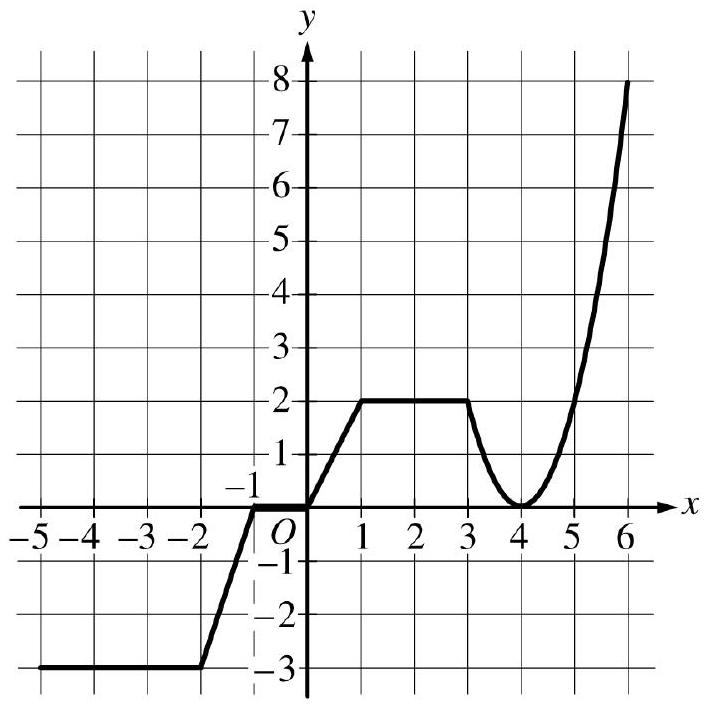
\includegraphics[width=0.6\linewidth]{figures/bc-2018_fig1.jpg}
\end{center}

Graph of $g$\\
The graph of the continuous function $g$, the derivative of the function $f$, is shown above. The function $g$ is piecewise linear for $-5 \leq x<3$, and $g(x)=2(x-4)^{2}$ for $3 \leq x \leq 6$.\\
\begin{parts}
\part If $f(1)=3$, what is the value of $f(-5)$ ?
\part Evaluate $\int_{1}^{6} g(x) d x$.
\part For $-5<x<6$, on what open intervals, if any, is the graph of $f$ both increasing and concave up? Give a reason for your answer.
\part Find the $x$-coordinate of each point of inflection of the graph of $f$. Give a reason for your answer.
\end{parts}
\begin{solution}
\begin{parts}
\part $f(-5)=f(1)+\int_{1}^{-5} g(x) d x=f(1)-\int_{-5}^{1} g(x) d x$

\[=3-\left(-9-\frac{3}{2}+1\right)=3-\left(-\frac{19}{2}\right)=\frac{25}{2}\]
\part $\int_{1}^{6} g(x) d x=\int_{1}^{3} g(x) d x+\int_{3}^{6} g(x) d x$

\[\begin{aligned}
& =\int_{1}^{3} 2 d x+\int_{3}^{6} 2(x-4)^{2} d x \\
& =4+\left[\frac{2}{3}(x-4)^{3}\right]_{x=3}^{x=6}=4+\frac{16}{3}-\left(-\frac{2}{3}\right)=10
\end{aligned}\]
\part The graph of $f$ is increasing and concave up on $0<x<1$ and $4<x<6$ because $f^{\prime}(x)=g(x)>0$ and $f^{\prime}(x)=g(x)$ is increasing on those intervals.
\part The graph of $f$ has a point of inflection at $x=4$ because $f^{\prime}(x)=g(x)$ changes from decreasing to increasing at $x=4$.
\end{parts}
\par\medskip
\textbf{Rubric:}\par
\begin{parts}
\part $2:\left\{\begin{array}{l}
1: \text { integral } \\
1: \text { answer }
\end{array}\right.$
\part $3:\left\{\begin{array}{l}1: \text { split at } x=3 \\ 1: \text { antiderivative of } 2(x-4)^{2} \\ 1: \text { answer }\end{array}\right.$
\part $2:\left\{\begin{array}{l}1: \text { intervals } \\ 1: \text { reason }\end{array}\right.$
\part $2:\left\{\begin{array}{l}
1: \text { answer } \\
1: \text { reason }
\end{array}\right.$
\end{parts}
\end{solution}

\question
% Q4 | 2018 Calculus BC | Part B | Calculator Prohibited
\begin{center}
\begin{tabular}{|c||c|c|c|c|c|}
\hline
\begin{tabular}{c}
$t$ \\
(years) \\
\end{tabular} & 2 & 3 & 5 & 7 & 10 \\
\hline
\begin{tabular}{c}
$H(t)$ \\
(meters) \\
\end{tabular} & 1.5 & 2 & 6 & 11 & 15 \\
\hline
\end{tabular}
\end{center}
The height of a tree at time $t$ is given by a twice-differentiable function $H$, where $H(t)$ is measured in meters and $t$ is measured in years. Selected values of $H(t)$ are given in the table above.\\
\begin{parts}
\part Use the data in the table to estimate $H^{\prime}(6)$. Using correct units, interpret the meaning of $H^{\prime}(6)$ in the context of the problem.
\part Explain why there must be at least one time $t$, for $2<t<10$, such that $H^{\prime}(t)=2$.
\part Use a trapezoidal sum with the four subintervals indicated by the data in the table to approximate the average height of the tree over the time interval $2 \leq t \leq 10$.
\part The height of the tree, in meters, can also be modeled by the function $G$, given by $G(x)=\frac{100 x}{1+x}$, where $x$ is the diameter of the base of the tree, in meters. When the tree is 50 meters tall, the diameter of the base of the tree is increasing at a rate of 0.03 meter per year. According to this model, what is the rate of change of the height of the tree with respect to time, in meters per year, at the time when the tree is 50 meters tall?
\end{parts}
\begin{solution}
\begin{parts}
\part $H^{\prime}(6) \approx \frac{H(7)-H(5)}{7-5}=\frac{11-6}{2}=\frac{5}{2}$\\
$H^{\prime}(6)$ is the rate at which the height of the tree is changing, in meters per year, at time $t=6$ years.
\part $\frac{H(5)-H(3)}{5-3}=\frac{6-2}{2}=2$

Because $H$ is differentiable on $3 \leq t \leq 5, H$ is continuous on $3 \leq t \leq 5$.

By the Mean Value Theorem, there exists a value $c, 3<c<5$, such that $H^{\prime}(c)=2$.
\part The average height of the tree over the time interval $2 \leq t \leq 10$ is given by $\frac{1}{10-2} \int_{2}^{10} H(t) d t$.

\[\begin{aligned}
\frac{1}{8} \int_{2}^{10} H(t) d t & \approx \frac{1}{8}\left(\frac{1.5+2}{2} \cdot 1+\frac{2+6}{2} \cdot 2+\frac{6+11}{2} \cdot 2+\frac{11+15}{2} \cdot 3\right) \\
& =\frac{1}{8}(65.75)=\frac{263}{32}
\end{aligned}\]

The average height of the tree over the time interval $2 \leq t \leq 10$ is $\frac{263}{32}$ meters.
\part $G(x)=50 \Rightarrow x=1$

\begin{align*}& \frac{d}{d t}(G(x))=\frac{d}{d x}(G(x)) \cdot \frac{d x}{d t}=\frac{(1+x) 100-100 x \cdot 1}{(1+x)^{2}} \cdot \frac{d x}{d t}=\frac{100}{(1+x)^{2}} \cdot \frac{d x}{d t} \\
& \left.\frac{d}{d t}(G(x))\right|_{x=1}=\frac{100}{(1+1)^{2}} \cdot 0.03=\frac{3}{4}\end{align*}

According to the model, the rate of change of the height of the tree with respect to time when the tree is 50 meters tall is $\frac{3}{4}$ meter per year.
\end{parts}
\par\medskip
\textbf{Rubric:}\par
\begin{parts}
\part $2:\left\{\begin{array}{l}1: \text { estimate } \\ 1: \text { interpretation with units }\end{array}\right.$
\part $2:\left\{\begin{aligned} 1: & \frac{H(5)-H(3)}{5-3} \\ 1: \text { conclusion using } & \\ & \text { Mean Value Theorem }\end{aligned}\right.$
\part $2:\left\{\begin{array}{l}1: \text { trapezoidal sum } \\ 1: \text { approximation }\end{array}\right.$
\part $3:\left\{\begin{array}{l}2: \frac{d}{d t}(G(x)) \\ 1: \text { answer }\end{array}\right.$
\part Note: $\max 1 / 3[1-0]$ if no chain rule
\end{parts}
\end{solution}

\question
% Q5 | 2018 Calculus BC | Part B | Calculator Prohibited
\begin{center}
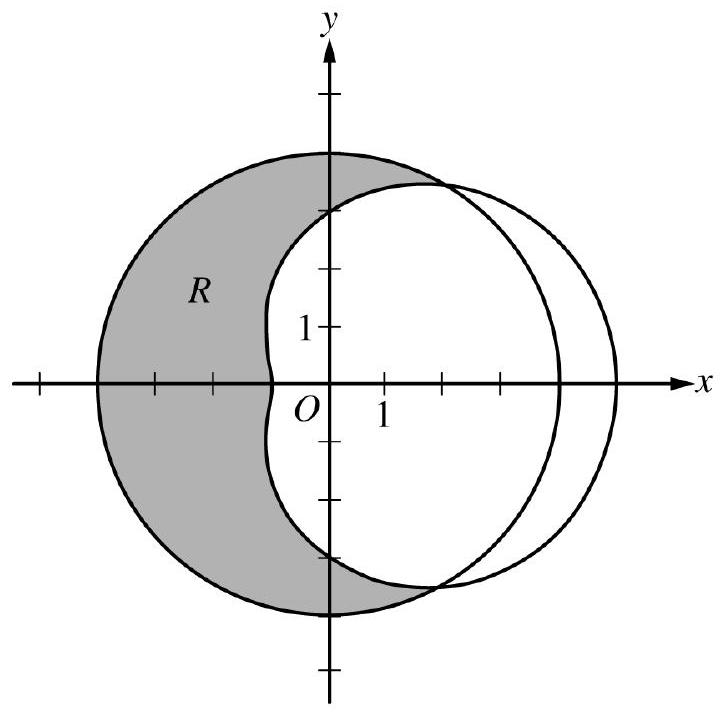
\includegraphics[width=0.6\linewidth]{figures/bc-2018_fig2.jpg}
\end{center}
The graphs of the polar curves $r=4$ and $r=3+2 \cos \theta$ are shown in the figure above. The curves intersect at $\theta=\frac{\pi}{3}$ and $\theta=\frac{5 \pi}{3}$.\\
\begin{parts}
\part Let $R$ be the shaded region that is inside the graph of $r=4$ and also outside the graph of $r=3+2 \cos \theta$, as shown in the figure above. Write an expression involving an integral for the area of $R$.
\part Find the slope of the line tangent to the graph of $r=3+2 \cos \theta$ at $\theta=\frac{\pi}{2}$.
\part A particle moves along the portion of the curve $r=3+2 \cos \theta$ for $0<\theta<\frac{\pi}{2}$. The particle moves in such a way that the distance between the particle and the origin increases at a constant rate of 3 units per second. Find the rate at which the angle $\theta$ changes with respect to time at the instant when the position of the particle corresponds to $\theta=\frac{\pi}{3}$. Indicate units of measure.
\end{parts}
\begin{solution}
\begin{parts}
\part Area $=\frac{1}{2} \int_{\pi / 3}^{5 \pi / 3}\left(4^{2}-(3+2 \cos \theta)^{2}\right) d \theta$
\part $\frac{d r}{d \theta}=-\left.2 \sin \theta \Rightarrow \frac{d r}{d \theta}\right|_{\theta=\pi / 2}=-2$\\
$r\left(\frac{\pi}{2}\right)=3+2 \cos \left(\frac{\pi}{2}\right)=3$\\
$y=r \sin \theta \Rightarrow \frac{d y}{d \theta}=\frac{d r}{d \theta} \sin \theta+r \cos \theta$\\
$x=r \cos \theta \Rightarrow \frac{d x}{d \theta}=\frac{d r}{d \theta} \cos \theta-r \sin \theta$\\
$\left.\frac{d y}{d x}\right|_{\theta=\pi / 2}=\left.\frac{d y / d \theta}{d x / d \theta}\right|_{\theta=\pi / 2}=\frac{-2 \sin \left(\frac{\pi}{2}\right)+3 \cos \left(\frac{\pi}{2}\right)}{-2 \cos \left(\frac{\pi}{2}\right)-3 \sin \left(\frac{\pi}{2}\right)}=\frac{2}{3}$\\
The slope of the line tangent to the graph of $r=3+2 \cos \theta$ at $\theta=\frac{\pi}{2}$ is $\frac{2}{3}$.\\
— OR —\\
$y=r \sin \theta=(3+2 \cos \theta) \sin \theta \Rightarrow \frac{d y}{d \theta}=3 \cos \theta+2 \cos ^{2} \theta-2 \sin ^{2} \theta$\\
$x=r \cos \theta=(3+2 \cos \theta) \cos \theta \Rightarrow \frac{d x}{d \theta}=-3 \sin \theta-4 \sin \theta \cos \theta$\\
$\left.\frac{d y}{d x}\right|_{\theta=\pi / 2}=\left.\frac{d y / d \theta}{d x / d \theta}\right|_{\theta=\pi / 2}=\frac{3 \cos \left(\frac{\pi}{2}\right)+2 \cos ^{2}\left(\frac{\pi}{2}\right)-2 \sin ^{2}\left(\frac{\pi}{2}\right)}{-3 \sin \left(\frac{\pi}{2}\right)-4 \sin \left(\frac{\pi}{2}\right) \cos \left(\frac{\pi}{2}\right)}=\frac{2}{3}$\\
The slope of the line tangent to the graph of $r=3+2 \cos \theta$ at $\theta=\frac{\pi}{2}$ is $\frac{2}{3}$.
\part $\frac{d r}{d t}=\frac{d r}{d \theta} \cdot \frac{d \theta}{d t}=-2 \sin \theta \cdot \frac{d \theta}{d t} \Rightarrow \frac{d \theta}{d t}=\frac{d r}{d t} \cdot \frac{1}{-2 \sin \theta}$\\
$\left.\frac{d \theta}{d t}\right|_{\theta=\pi / 3}=3 \cdot \frac{1}{-2 \sin \left(\frac{\pi}{3}\right)}=\frac{3}{-\sqrt{3}}=-\sqrt{3}$ radians per second
\end{parts}
\par\medskip
\textbf{Rubric:}\par
\begin{parts}
\part $3:\left\{\begin{array}{l}1: \text { constant and limits } \\ 2: \text { integrand }\end{array}\right.$
\part $3:\left\{\begin{array}{c}1: \frac{d y}{d \theta}=\frac{d r}{d \theta} \sin \theta+r \cos \theta \\ \text { or } \frac{d x}{d \theta}=\frac{d r}{d \theta} \cos \theta-r \sin \theta \\ 1: \frac{d y}{d x}=\frac{d r}{d \theta} \sin \theta+r \cos \theta \\ 1: \text { answer }\end{array}\right.$
\part $3:\left\{\begin{array}{l}1: \frac{d r}{d t}=\frac{d r}{d \theta} \cdot \frac{d \theta}{d t} \\ 1: \frac{d \theta}{d t}=\frac{d r}{d t} \cdot \frac{1}{-2 \sin \theta} \\ 1: \text { answer with units }\end{array}\right.$
\end{parts}
\end{solution}

\question
% Q6 | 2018 Calculus BC | Part B | Calculator Prohibited
The Maclaurin series for $\ln (1+x)$ is given by
\[x-\frac{x^{2}}{2}+\frac{x^{3}}{3}-\frac{x^{4}}{4}+\cdots+(-1)^{n+1} \frac{x^{n}}{n}+\cdots\]

On its interval of convergence, this series converges to $\ln (1+x)$. Let $f$ be the function defined by

\[f(x)=x \ln \left(1+\frac{x}{3}\right)\]
\begin{parts}
\part Write the first four nonzero terms and the general term of the Maclaurin series for $f$.
\part Determine the interval of convergence of the Maclaurin series for $f$. Show the work that leads to your answer.
\part Let $P_{4}(x)$ be the fourth-degree Taylor polynomial for $f$ about $x=0$. Use the alternating series error bound to find an upper bound for $\left|P_{4}(2)-f(2)\right|$.
\end{parts}
\begin{solution}
\begin{parts}
\part The first four nonzero terms are $\frac{x^{2}}{3}-\frac{x^{3}}{2 \cdot 3^{2}}+\frac{x^{4}}{3 \cdot 3^{3}}-\frac{x^{5}}{4 \cdot 3^{4}}$.

The general term is $(-1)^{n+1} \frac{x^{n+1}}{n \cdot 3^{n}}$.
\part $\lim _{n \rightarrow \infty}\left|\frac{\frac{(-1)^{n+2} x^{n+2}}{(n+1)\left(3^{n+1}\right)}}{\frac{(-1)^{n+1} x^{n+1}}{n \cdot 3^{n}}}\right|=\lim _{n \rightarrow \infty}\left|\frac{-x}{3} \cdot \frac{n}{(n+1)}\right|=\left|\frac{x}{3}\right|$\\
$\left|\frac{x}{3}\right|<1$ for $|x|<3$\\
Therefore, the radius of convergence of the Maclaurin series for $f$ is 3 .\\
— OR —\\
The radius of convergence of the Maclaurin series for $\ln (1+x)$ is 1 , so the series for $f(x)=x \ln \left(1+\frac{x}{3}\right)$ converges absolutely for $\left|\frac{x}{3}\right|<1$.\\
$\left|\frac{x}{3}\right|<1 \Rightarrow|x|<3$\\
Therefore, the radius of convergence of the Maclaurin series for $f$ is 3 .\\
When $x=-3$, the series is $\sum_{n=1}^{\infty}(-1)^{n+1} \frac{(-3)^{n+1}}{n \cdot 3^{n}}=\sum_{n=1}^{\infty} \frac{3}{n}$, which diverges by comparison to the harmonic series.

When $x=3$, the series is $\sum_{n=1}^{\infty}(-1)^{n+1} \frac{3^{n+1}}{n \cdot 3^{n}}=\sum_{n=1}^{\infty}(-1)^{n+1} \frac{3}{n}$, which converges by the alternating series test.

The interval of convergence of the Maclaurin series for $f$ is $-3<x \leq 3$.
\part By the alternating series error bound, an upper bound for $\left|P_{4}(2)-f(2)\right|$ is the magnitude of the next term of the alternating series.\\
$\left|P_{4}(2)-f(2)\right|<\left|-\frac{2^{5}}{4 \cdot 3^{4}}\right|=\frac{8}{81}$
\end{parts}
\par\medskip
\textbf{Rubric:}\par
\begin{parts}
\part $2:\left\{\begin{array}{l}1: \text { first four terms } \\ 1: \text { general term }\end{array}\right.$
\part $5:\left\{\begin{array}{l}1: \text { sets up ratio } \\ 1: \text { computes limit of ratio } \\ 1: \text { radius of convergence } \\ 1: \text { considers both endpoints } \\ 1: \text { analysis and interval of } \\ \quad \text { convergence }\end{array}\right.$
\part $5:\left\{\begin{array}{l}1: \text { radius for } \ln (1+x) \text { series } \\ 1: \text { substitutes } \frac{x}{3} \\ 1: \text { radius of convergence } \\ 1: \text { considers both endpoints } \\ 1: \text { analysis and interval of } \\ \quad \text { convergence }\end{array}\right.$
\part $2:\left\{\begin{array}{c}1: \text { uses fifth-degree term } \\ \quad \text { as error bound } \\ 1: \text { answer }\end{array}\right.$
\end{parts}
\end{solution}

\end{questions}

\section*{2019 AP Calculus BC}

\begin{questions}

\question
% Q1 | 2019 Calculus BC | Part A | Calculator Active
Fish enter a lake at a rate modeled by the function $E$ given by $E(t)=20+15 \sin \left(\frac{\pi t}{6}\right)$. Fish leave the lake at a rate modeled by the function $L$ given by $L(t)=4+2^{0.1 t^{2}}$. Both $E(t)$ and $L(t)$ are measured in fish per hour, and $t$ is measured in hours since midnight $(t=0)$.\\
\begin{parts}
\part How many fish enter the lake over the 5 -hour period from midnight $(t=0)$ to 5 A.M. $(t=5)$ ? Give your answer to the nearest whole number.
\part What is the average number of fish that leave the lake per hour over the 5 -hour period from midnight $(t=0)$ to 5 A.M. $(t=5)$ ?
\part At what time $t$, for $0 \leq t \leq 8$, is the greatest number of fish in the lake? Justify your answer.
\part Is the rate of change in the number of fish in the lake increasing or decreasing at 5 A.M. ( $t=5$ ) ? Explain your reasoning.
\end{parts}
\begin{solution}
\begin{parts}
\part $\int_{0}^{5} E(t) d t=153.457690$

To the nearest whole number, 153 fish enter the lake from midnight to 5 A.M.
\part $\frac{1}{5-0} \int_{0}^{5} L(t) d t=6.059038$

The average number of fish that leave the lake per hour from midnight to 5 A.M. is 6.059 fish per hour.
\part The rate of change in the number of fish in the lake at time $t$ is given by $E(t)-L(t)$.\\
$E(t)-L(t)=0 \Rightarrow t=6.20356$\\
$E(t)-L(t)>0$ for $0 \leq t<6.20356$, and $E(t)-L(t)<0$ for $6.20356<t \leq 8$. Therefore the greatest number of fish in the lake is at time $t=6.204$ (or 6.203).

Let $A(t)$ be the change in the number of fish in the lake from midnight to $t$ hours after midnight.

\begin{align*}& A(t)=\int_{0}^{t}(E(s)-L(s)) d s \\
& A^{\prime}(t)=E(t)-L(t)=0 \Rightarrow t=C=6.20356\end{align*}

\begin{center}
\begin{tabular}{c|c}
$t$ & $A(t)$ \\
\hline
0 & 0 \\
$C$ & 135.01492 \\
8 & 80.91998 \\
\end{tabular}
\end{center}

Therefore the greatest number of fish in the lake is at time $t=6.204$ (or 6.203).
\part $E^{\prime}(5)-L^{\prime}(5)=-10.7228<0$

Because $E^{\prime}(5)-L^{\prime}(5)<0$, the rate of change in the number of fish is decreasing at time $t=5$.
\end{parts}
\par\medskip
\textbf{Rubric:}\par
\begin{parts}
\part $2:\left\{\begin{array}{l}1: \text { integral } \\ 1: \text { answer }\end{array}\right.$
\part $2:\left\{\begin{array}{l}1: \text { integral } \\ 1: \text { answer }\end{array}\right.$
\part $3:\left\{\begin{array}{l}1: \text { sets } E(t)-L(t)=0 \\ 1: \text { answer } \\ 1: \text { justification }\end{array}\right.$
\part $2:\left\{\begin{array}{l}1: \text { considers } E^{\prime}(5) \text { and } L^{\prime}(5) \\ 1: \text { answer with explanation }\end{array}\right.$
\end{parts}
\end{solution}

\question
% Q2 | 2019 Calculus BC | Part A | Calculator Active
\begin{center}
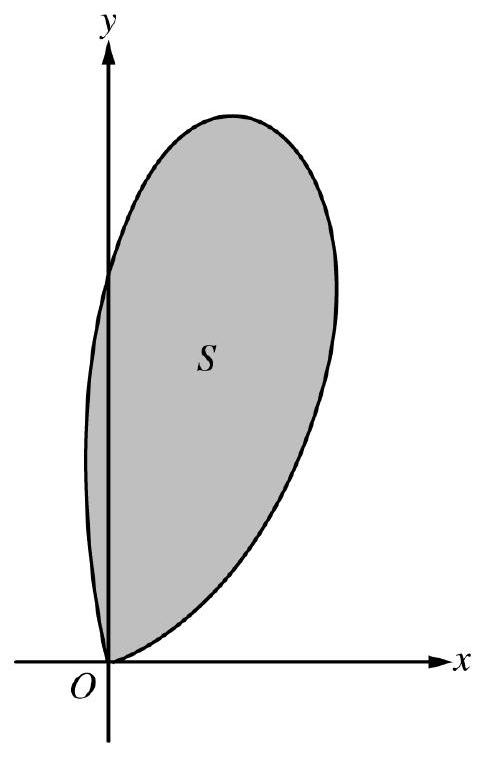
\includegraphics[width=0.6\linewidth]{figures/bc-2019_fig1.jpg}
\end{center}
Let $S$ be the region bounded by the graph of the polar curve $r(\theta)=3 \sqrt{\theta} \sin \left(\theta^{2}\right)$ for $0 \leq \theta \leq \sqrt{\pi}$, as shown in the figure above.\\
\begin{parts}
\part Find the area of $S$.
\part What is the average distance from the origin to a point on the polar curve $r(\theta)=3 \sqrt{\theta} \sin \left(\theta^{2}\right)$ for $0 \leq \theta \leq \sqrt{\pi} ?$
\part There is a line through the origin with positive slope $m$ that divides the region $S$ into two regions with equal areas. Write, but do not solve, an equation involving one or more integrals whose solution gives the value of $m$.
\part For $k>0$, let $A(k)$ be the area of the portion of region $S$ that is also inside the circle $r=k \cos \theta$. Find $\lim _{k \rightarrow \infty} A(k)$.
\end{parts}
\begin{solution}
\begin{parts}
\part $\frac{1}{2} \int_{0}^{\sqrt{\pi}}(r(\theta))^{2} d \theta=3.534292$

The area of $S$ is 3.534 .
\part $\frac{1}{\sqrt{\pi}-0} \int_{0}^{\sqrt{\pi}} r(\theta) d \theta=1.579933$

The average distance from the origin to a point on the curve $r=r(\theta)$ for $0 \leq \theta \leq \sqrt{\pi}$ is 1.580 (or 1.579).
\part $\tan \theta=\frac{y}{x}=m \Rightarrow \theta=\tan ^{-1} m$

\[\frac{1}{2} \int_{0}^{\tan ^{-1} m}(r(\theta))^{2} d \theta=\frac{1}{2}\left(\frac{1}{2} \int_{0}^{\sqrt{\pi}}(r(\theta))^{2} d \theta\right)\]
\part As $k \rightarrow \infty$, the circle $r=k \cos \theta$ grows to enclose all points to the right of the $y$-axis.

\[\begin{aligned}
\lim _{k \rightarrow \infty} A(k) & =\frac{1}{2} \int_{0}^{\pi / 2}(r(\theta))^{2} d \theta \\
& =\frac{1}{2} \int_{0}^{\pi / 2}\left(3 \sqrt{\theta} \sin \left(\theta^{2}\right)\right)^{2} d \theta=3.324
\end{aligned}\]
\end{parts}
\par\medskip
\textbf{Rubric:}\par
\begin{parts}
\part $2:\left\{\begin{array}{l}
1: \text { integral } \\
1: \text { answer }
\end{array}\right.$
\part $2:\left\{\begin{array}{l}1: \text { integral } \\ 1: \text { answer }\end{array}\right.$
\part $3:\left\{\begin{aligned} 1: & \text { equates polar areas } \\ 1: & \text { inverse trigonometric function } \\ & \text { applied to } m \text { as limit of } \\ & \text { integration } \\ 1: & \text { equation }\end{aligned}\right.$
\part $2:\left\{\begin{array}{l}1: \text { limits of integration } \\ 1: \text { answer with integral }\end{array}\right.$
\end{parts}
\end{solution}

\question
% Q3 | 2019 Calculus BC | Part B | Calculator Prohibited
\begin{center}
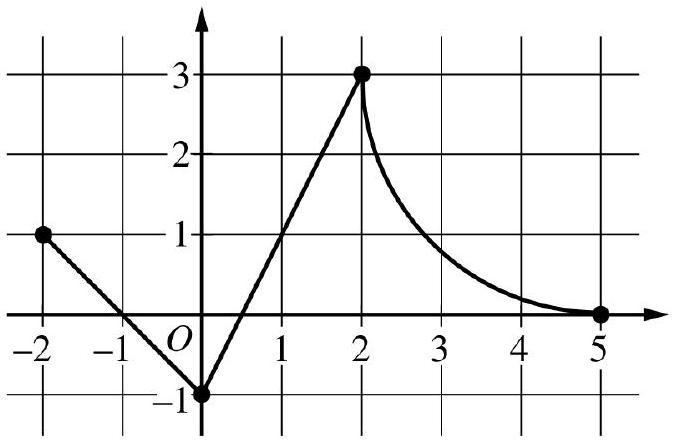
\includegraphics[width=0.6\linewidth]{figures/bc-2019_fig2.jpg}
\end{center}

Graph of $f$\\
The continuous function $f$ is defined on the closed interval $-6 \leq x \leq 5$. The figure above shows a portion of the graph of $f$, consisting of two line segments and a quarter of a circle centered at the point $(5,3)$. It is known that the point ( $3,3-\sqrt{5}$ ) is on the graph of $f$.\\
\begin{parts}
\part If $\int_{-6}^{5} f(x) d x=7$, find the value of $\int_{-6}^{-2} f(x) d x$. Show the work that leads to your answer.
\part Evaluate $\int_{3}^{5}\left(2 f^{\prime}(x)+4\right) d x$.
\part The function $g$ is given by $g(x)=\int_{-2}^{x} f(t) d t$. Find the absolute maximum value of $g$ on the interval $-2 \leq x \leq 5$. Justify your answer.
\part Find $\lim _{x \rightarrow 1} \frac{10^{x}-3 f^{\prime}(x)}{f(x)-\arctan x}$.
\end{parts}
\begin{solution}
\begin{parts}
\part $\int_{-6}^{5} f(x) d x=\int_{-6}^{-2} f(x) d x+\int_{-2}^{5} f(x) d x$

\[\begin{aligned}
& \Rightarrow 7=\int_{-6}^{-2} f(x) d x+2+\left(9-\frac{9 \pi}{4}\right) \\
& \Rightarrow \int_{-6}^{-2} f(x) d x=7-\left(11-\frac{9 \pi}{4}\right)=\frac{9 \pi}{4}-4
\end{aligned}\]
\part $\int_{3}^{5}\left(2 f^{\prime}(x)+4\right) d x=2 \int_{3}^{5} f^{\prime}(x) d x+\int_{3}^{5} 4 d x$

\begin{align*}& =2(f(5)-f(3))+4(5-3) \\
& =2(0-(3-\sqrt{5}))+8 \\
& =2(-3+\sqrt{5})+8=2+2 \sqrt{5}\end{align*}

OR -
\[\begin{aligned}
\int_{3}^{5}\left(2 f^{\prime}(x)+4\right) d x & =[2 f(x)+4 x]_{x=3}^{x=5} \\
& =(2 f(5)+20)-(2 f(3)+12) \\
& =(2 \cdot 0+20)-(2(3-\sqrt{5})+12) \\
& =2+2 \sqrt{5}
\end{aligned}\]
\part $g^{\prime}(x)=f(x)=0 \Rightarrow x=-1, x=\frac{1}{2}, x=5$

\begin{center}
\begin{tabular}{c|c}
$x$ & $g(x)$ \\
\hline
-2 & 0 \\
-1 & $\frac{1}{2}$ \\
$\frac{1}{2}$ & $-\frac{1}{4}$ \\
5 & $11-\frac{9 \pi}{4}$ \\
\end{tabular}
\end{center}

On the interval $-2 \leq x \leq 5$, the absolute maximum value of $g$ is $g(5)=11-\frac{9 \pi}{4}$.
\part $\lim _{x \rightarrow 1} \frac{10^{x}-3 f^{\prime}(x)}{f(x)-\arctan x}=\frac{10^{1}-3 f^{\prime}(1)}{f(1)-\arctan 1}$

\[=\frac{10-3 \cdot 2}{1-\arctan 1}=\frac{4}{1-\frac{\pi}{4}}\]

3: $\left\{\begin{array}{l}1: \int_{-6}^{5} f(x) d x=\int_{-6}^{-2} f(x) d x+\int_{-2}^{5} f(x) d x \\ 1: \int_{-2}^{5} f(x) d x \\ 1: \text { answer }\end{array}\right.$
\end{parts}
\par\medskip
\textbf{Rubric:}\par
\begin{parts}
\part $2:\left\{\begin{array}{l}1: \text { Fundamental Theorem of Calculus } \\ 1: \text { answer }\end{array}\right.$
\part $3:\left\{\begin{array}{l}1: g^{\prime}(x)=f(x) \\ 1: \text { identifies } x=-1 \text { as a candidate } \\ 1: \text { answer with justification }\end{array}\right.$
\end{parts}
\end{solution}

\question
% Q4 | 2019 Calculus BC | Part B | Calculator Prohibited
\begin{center}
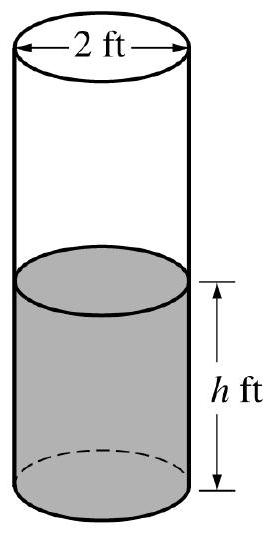
\includegraphics[width=0.6\linewidth]{figures/bc-2019_fig3.jpg}
\end{center}
A cylindrical barrel with a diameter of 2 feet contains collected rainwater, as shown in the figure above. The water drains out through a valve (not shown) at the bottom of the barrel. The rate of change of the height $h$ of the water in the barrel with respect to time $t$ is modeled by $\frac{d h}{d t}=-\frac{1}{10} \sqrt{h}$, where $h$ is measured in feet and $t$ is measured in seconds. (The volume $V$ of a cylinder with radius $r$ and height $h$ is $V=\pi r^{2} h$.)\\
\begin{parts}
\part Find the rate of change of the volume of water in the barrel with respect to time when the height of the water is 4 feet. Indicate units of measure.
\part When the height of the water is 3 feet, is the rate of change of the height of the water with respect to time increasing or decreasing? Explain your reasoning.
\part At time $t=0$ seconds, the height of the water is 5 feet. Use separation of variables to find an expression for $h$ in terms of $t$.
\end{parts}
\begin{solution}
\begin{parts}
\part $V=\pi r^{2} h=\pi(1)^{2} h=\pi h$\\
$\left.\frac{d V}{d t}\right|_{h=4}=\left.\pi \frac{d h}{d t}\right|_{h=4}=\pi\left(-\frac{1}{10} \sqrt{4}\right)=-\frac{\pi}{5}$ cubic feet per second
\part $\frac{d^{2} h}{d t^{2}}=-\frac{1}{20 \sqrt{h}} \cdot \frac{d h}{d t}=-\frac{1}{20 \sqrt{h}} \cdot\left(-\frac{1}{10} \sqrt{h}\right)=\frac{1}{200}$

Because $\frac{d^{2} h}{d t^{2}}=\frac{1}{200}>0$ for $h>0$, the rate of change of the height is increasing when the height of the water is 3 feet.
\part $\frac{d h}{\sqrt{h}}=-\frac{1}{10} d t$

\[\begin{aligned}
& \int \frac{d h}{\sqrt{h}}=\int-\frac{1}{10} d t \\
& 2 \sqrt{h}=-\frac{1}{10} t+C \\
& 2 \sqrt{5}=-\frac{1}{10} \cdot 0+C \Rightarrow C=2 \sqrt{5} \\
& 2 \sqrt{h}=-\frac{1}{10} t+2 \sqrt{5} \\
& h(t)=\left(-\frac{1}{20} t+\sqrt{5}\right)^{2}
\end{aligned}\]
\end{parts}
\par\medskip
\textbf{Rubric:}\par
\begin{parts}
\part $2:\left\{\begin{array}{l}1: \frac{d V}{d t}=\pi \frac{d h}{d t} \\ 1: \text { answer with units }\end{array}\right.$
\part $3:\left\{\begin{array}{l}1: \frac{d}{d h}\left(-\frac{1}{10} \sqrt{h}\right)=-\frac{1}{20 \sqrt{h}} \\ 1: \frac{d^{2} h}{d t^{2}}=-\frac{1}{20 \sqrt{h}} \cdot \frac{d h}{d t} \\ 1: \text { answer with explanation }\end{array}\right.$
\part $4:\left\{\begin{array}{l}1: \text { separation of variables } \\ 1: \text { antiderivatives } \\ 1: \text { constant of integration } \\ \text { and uses initial condition } \\ 1: h(t)\end{array}\right.$
\part Note: 0/4 if no separation of variables
\part Note: max 2 / 4 [1-1-0-0] if no constant of integration
\end{parts}
\end{solution}

\question
% Q5 | 2019 Calculus BC | Part B | Calculator Prohibited
Consider the family of functions $f(x)=\frac{1}{x^{2}-2 x+k}$, where $k$ is a constant.\\

\begin{center}
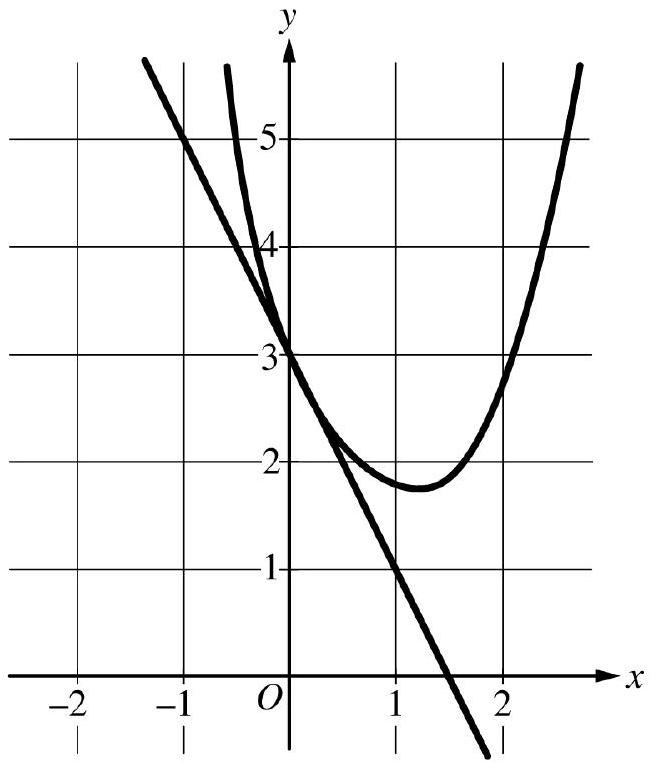
\includegraphics[width=0.6\linewidth]{figures/bc-2019_fig4.jpg}
\end{center}
\begin{parts}
\part Find the value of $k$, for $k>0$, such that the slope of the line tangent to the graph of $f$ at $x=0$ equals 6 .
\part For $k=-8$, find the value of $\int_{0}^{1} f(x) d x$.
\part For $k=1$, find the value of $\int_{0}^{2} f(x) d x$ or show that it diverges.\\
\end{parts}
\begin{solution}
\begin{parts}
\part $f^{\prime}(x)=\frac{-(2 x-2)}{\left(x^{2}-2 x+k\right)^{2}}$\\
$f^{\prime}(0)=\frac{2}{k^{2}}=6 \Rightarrow k^{2}=\frac{1}{3} \Rightarrow k=\frac{1}{\sqrt{3}}$
\part $\frac{1}{x^{2}-2 x-8}=\frac{1}{(x-4)(x+2)}=\frac{A}{x-4}+\frac{B}{x+2}$

\[\begin{aligned}
& \Rightarrow 1=A(x+2)+B(x-4) \\
& \Rightarrow A=\frac{1}{6}, B=-\frac{1}{6} \\
& \begin{aligned}
\int_{0}^{1} f(x) d x & =\int_{0}^{1}\left(\frac{\frac{1}{6}}{x-4}-\frac{\frac{1}{6}}{x+2}\right) d x \\
& =\left[\frac{1}{6} \ln |x-4|-\frac{1}{6} \ln |x+2|\right]_{x=0}^{x=1} \\
& =\left(\frac{1}{6} \ln 3-\frac{1}{6} \ln 3\right)-\left(\frac{1}{6} \ln 4-\frac{1}{6} \ln 2\right)=-\frac{1}{6} \ln 2
\end{aligned}
\end{aligned}\]
\part $\int_{0}^{2} \frac{1}{x^{2}-2 x+1} d x=\int_{0}^{2} \frac{1}{(x-1)^{2}} d x=\int_{0}^{1} \frac{1}{(x-1)^{2}} d x+\int_{1}^{2} \frac{1}{(x-1)^{2}} d x$

\[\begin{aligned}
& =\lim _{b \rightarrow 1^{-}} \int_{0}^{b} \frac{1}{(x-1)^{2}} d x+\lim _{b \rightarrow 1^{+}} \int_{b}^{2} \frac{1}{(x-1)^{2}} d x \\
& =\lim _{b \rightarrow 1^{-}}\left(-\left.\frac{1}{x-1}\right|_{x=0} ^{x=b}\right)+\lim _{b \rightarrow 1^{+}}\left(-\left.\frac{1}{x-1}\right|_{x=b} ^{x=2}\right) \\
& =\lim _{b \rightarrow 1^{-}}\left(-\frac{1}{b-1}-1\right)+\lim _{b \rightarrow 1^{+}}\left(-1+\frac{1}{b-1}\right)
\end{aligned}\]

Because $\lim _{b \rightarrow 1^{-}}\left(-\frac{1}{b-1}\right)$ does not exist, the integral diverges.
\end{parts}
\par\medskip
\textbf{Rubric:}\par
\begin{parts}
\part $3:\left\{\begin{array}{l}1: \text { denominator of } f^{\prime}(x) \\ 1: f^{\prime}(x) \\ 1: \text { answer }\end{array}\right.$
\part $3:\left\{\begin{array}{r}1: \text { partial fraction } \\ \text { decomposition } \\ 1: \text { antiderivatives } \\ 1: \text { answer }\end{array}\right.$
\part $3:\left\{\begin{array}{l}1: \text { improper integral } \\ 1: \text { antiderivative } \\ 1: \text { answer with reason }\end{array}\right.$
\end{parts}
\end{solution}

\question
% Q6 | 2019 Calculus BC | Part B | Calculator Prohibited
\begin{center}
\begin{tabular}{|c|c|}
\hline
$n$ & $f^{(n)}(0)$ \\
\hline\hline
2 & 3 \\
\hline
3 & $-\frac{23}{2}$ \\
\hline
4 & 54 \\
\hline
\end{tabular}
\end{center}
A function $f$ has derivatives of all orders for all real numbers $x$. A portion of the graph of $f$ is shown above, along with the line tangent to the graph of $f$ at $x=0$. Selected derivatives of $f$ at $x=0$ are given in the table above.\\
\begin{parts}
\part Write the third-degree Taylor polynomial for $f$ about $x=0$.
\part Write the first three nonzero terms of the Maclaurin series for $e^{x}$. Write the second-degree Taylor polynomial for $e^{x} f(x)$ about $x=0$.
\part Let $h$ be the function defined by $h(x)=\int_{0}^{x} f(t) d t$. Use the Taylor polynomial found in part (a) to find an approximation for $h(1)$.
\part It is known that the Maclaurin series for $h$ converges to $h(x)$ for all real numbers $x$. It is also known that the individual terms of the series for $h(1)$ alternate in sign and decrease in absolute value to 0 . Use the alternating series error bound to show that the approximation found in part (c) differs from $h(1)$ by at most 0.45 .
\end{parts}
\begin{solution}
\begin{parts}
\part $f(0)=3$ and $f^{\prime}(0)=-2$

The third-degree Taylor polynomial for $f$ about $x=0$ is\\
$3-2 x+\frac{3}{2!} x^{2}+\frac{-\frac{23}{2}}{3!} x^{3}=3-2 x+\frac{3}{2} x^{2}-\frac{23}{12} x^{3}$.
\part The first three nonzero terms of the Maclaurin series for $e^{x}$ are

\[1+x+\frac{1}{2!} x^{2}\]

The second-degree Taylor polynomial for $e^{x} f(x)$ about $x=0$ is

\[\begin{aligned}
3(1 & \left.+x+\frac{1}{2!} x^{2}\right)-2 x(1+x)+\frac{3}{2} x^{2}(1) \\
& =3+(3-2) x+\left(\frac{3}{2}-2+\frac{3}{2}\right) x^{2} \\
& =3+x+x^{2}
\end{aligned}\]
\part $h(1)=\int_{0}^{1} f(t) d t$

\[\begin{aligned}
& \approx \int_{0}^{1}\left(3-2 t+\frac{3}{2} t^{2}-\frac{23}{12} t^{3}\right) d t \\
& =\left[3 t-t^{2}+\frac{1}{2} t^{3}-\frac{23}{48} t^{4}\right]_{t=0}^{t=1} \\
& =3-1+\frac{1}{2}-\frac{23}{48}=\frac{97}{48}
\end{aligned}\]
\part The alternating series error bound is the absolute value of the first omitted term of the series for $h(1)$.

\[\int_{0}^{1}\left(\frac{54}{4!} t^{4}\right) d t=\left[\frac{9}{20} t^{5}\right]_{t=0}^{t=1}=\frac{9}{20}\]

Error $\leq\left|\frac{9}{20}\right|=0.45$
\end{parts}
\par\medskip
\textbf{Rubric:}\par
\begin{parts}
\part $2:\left\{\begin{array}{l}1: \text { two terms } \\ 1: \text { remaining terms }\end{array}\right.$
\part $2:\left\{\begin{array}{l}1: \text { three terms for } e^{x} \\ 1: \text { three terms for } e^{x} f(x)\end{array}\right.$
\part $2:\left\{\begin{array}{l}1: \text { antiderivative } \\ 1: \text { answer }\end{array}\right.$
\part $3:\left\{\begin{array}{l}1: \text { uses fourth-degree term } \\ \text { of Maclaurin series for } f \\ 1: \text { uses first omitted term } \\ \text { of series for } h(1) \\ 1: \text { error bound }\end{array}\right.$
\end{parts}
\end{solution}

\end{questions}

\end{document}
